% Options for packages loaded elsewhere
\PassOptionsToPackage{unicode}{hyperref}
\PassOptionsToPackage{hyphens}{url}
%
\documentclass[
]{book}
\usepackage{lmodern}
\usepackage{amsmath}
\usepackage{ifxetex,ifluatex}
\ifnum 0\ifxetex 1\fi\ifluatex 1\fi=0 % if pdftex
  \usepackage[T1]{fontenc}
  \usepackage[utf8]{inputenc}
  \usepackage{textcomp} % provide euro and other symbols
  \usepackage{amssymb}
\else % if luatex or xetex
  \usepackage{unicode-math}
  \defaultfontfeatures{Scale=MatchLowercase}
  \defaultfontfeatures[\rmfamily]{Ligatures=TeX,Scale=1}
\fi
% Use upquote if available, for straight quotes in verbatim environments
\IfFileExists{upquote.sty}{\usepackage{upquote}}{}
\IfFileExists{microtype.sty}{% use microtype if available
  \usepackage[]{microtype}
  \UseMicrotypeSet[protrusion]{basicmath} % disable protrusion for tt fonts
}{}
\makeatletter
\@ifundefined{KOMAClassName}{% if non-KOMA class
  \IfFileExists{parskip.sty}{%
    \usepackage{parskip}
  }{% else
    \setlength{\parindent}{0pt}
    \setlength{\parskip}{6pt plus 2pt minus 1pt}}
}{% if KOMA class
  \KOMAoptions{parskip=half}}
\makeatother
\usepackage{xcolor}
\IfFileExists{xurl.sty}{\usepackage{xurl}}{} % add URL line breaks if available
\IfFileExists{bookmark.sty}{\usepackage{bookmark}}{\usepackage{hyperref}}
\hypersetup{
  pdftitle={Coding Your Future: A Guidebook for Students},
  pdfauthor={Duncan Hull and Bryan Mathers},
  hidelinks,
  pdfcreator={LaTeX via pandoc}}
\urlstyle{same} % disable monospaced font for URLs
\usepackage{color}
\usepackage{fancyvrb}
\newcommand{\VerbBar}{|}
\newcommand{\VERB}{\Verb[commandchars=\\\{\}]}
\DefineVerbatimEnvironment{Highlighting}{Verbatim}{commandchars=\\\{\}}
% Add ',fontsize=\small' for more characters per line
\usepackage{framed}
\definecolor{shadecolor}{RGB}{248,248,248}
\newenvironment{Shaded}{\begin{snugshade}}{\end{snugshade}}
\newcommand{\AlertTok}[1]{\textcolor[rgb]{0.94,0.16,0.16}{#1}}
\newcommand{\AnnotationTok}[1]{\textcolor[rgb]{0.56,0.35,0.01}{\textbf{\textit{#1}}}}
\newcommand{\AttributeTok}[1]{\textcolor[rgb]{0.77,0.63,0.00}{#1}}
\newcommand{\BaseNTok}[1]{\textcolor[rgb]{0.00,0.00,0.81}{#1}}
\newcommand{\BuiltInTok}[1]{#1}
\newcommand{\CharTok}[1]{\textcolor[rgb]{0.31,0.60,0.02}{#1}}
\newcommand{\CommentTok}[1]{\textcolor[rgb]{0.56,0.35,0.01}{\textit{#1}}}
\newcommand{\CommentVarTok}[1]{\textcolor[rgb]{0.56,0.35,0.01}{\textbf{\textit{#1}}}}
\newcommand{\ConstantTok}[1]{\textcolor[rgb]{0.00,0.00,0.00}{#1}}
\newcommand{\ControlFlowTok}[1]{\textcolor[rgb]{0.13,0.29,0.53}{\textbf{#1}}}
\newcommand{\DataTypeTok}[1]{\textcolor[rgb]{0.13,0.29,0.53}{#1}}
\newcommand{\DecValTok}[1]{\textcolor[rgb]{0.00,0.00,0.81}{#1}}
\newcommand{\DocumentationTok}[1]{\textcolor[rgb]{0.56,0.35,0.01}{\textbf{\textit{#1}}}}
\newcommand{\ErrorTok}[1]{\textcolor[rgb]{0.64,0.00,0.00}{\textbf{#1}}}
\newcommand{\ExtensionTok}[1]{#1}
\newcommand{\FloatTok}[1]{\textcolor[rgb]{0.00,0.00,0.81}{#1}}
\newcommand{\FunctionTok}[1]{\textcolor[rgb]{0.00,0.00,0.00}{#1}}
\newcommand{\ImportTok}[1]{#1}
\newcommand{\InformationTok}[1]{\textcolor[rgb]{0.56,0.35,0.01}{\textbf{\textit{#1}}}}
\newcommand{\KeywordTok}[1]{\textcolor[rgb]{0.13,0.29,0.53}{\textbf{#1}}}
\newcommand{\NormalTok}[1]{#1}
\newcommand{\OperatorTok}[1]{\textcolor[rgb]{0.81,0.36,0.00}{\textbf{#1}}}
\newcommand{\OtherTok}[1]{\textcolor[rgb]{0.56,0.35,0.01}{#1}}
\newcommand{\PreprocessorTok}[1]{\textcolor[rgb]{0.56,0.35,0.01}{\textit{#1}}}
\newcommand{\RegionMarkerTok}[1]{#1}
\newcommand{\SpecialCharTok}[1]{\textcolor[rgb]{0.00,0.00,0.00}{#1}}
\newcommand{\SpecialStringTok}[1]{\textcolor[rgb]{0.31,0.60,0.02}{#1}}
\newcommand{\StringTok}[1]{\textcolor[rgb]{0.31,0.60,0.02}{#1}}
\newcommand{\VariableTok}[1]{\textcolor[rgb]{0.00,0.00,0.00}{#1}}
\newcommand{\VerbatimStringTok}[1]{\textcolor[rgb]{0.31,0.60,0.02}{#1}}
\newcommand{\WarningTok}[1]{\textcolor[rgb]{0.56,0.35,0.01}{\textbf{\textit{#1}}}}
\usepackage{longtable,booktabs}
\usepackage{calc} % for calculating minipage widths
% Correct order of tables after \paragraph or \subparagraph
\usepackage{etoolbox}
\makeatletter
\patchcmd\longtable{\par}{\if@noskipsec\mbox{}\fi\par}{}{}
\makeatother
% Allow footnotes in longtable head/foot
\IfFileExists{footnotehyper.sty}{\usepackage{footnotehyper}}{\usepackage{footnote}}
\makesavenoteenv{longtable}
\usepackage{graphicx}
\makeatletter
\def\maxwidth{\ifdim\Gin@nat@width>\linewidth\linewidth\else\Gin@nat@width\fi}
\def\maxheight{\ifdim\Gin@nat@height>\textheight\textheight\else\Gin@nat@height\fi}
\makeatother
% Scale images if necessary, so that they will not overflow the page
% margins by default, and it is still possible to overwrite the defaults
% using explicit options in \includegraphics[width, height, ...]{}
\setkeys{Gin}{width=\maxwidth,height=\maxheight,keepaspectratio}
% Set default figure placement to htbp
\makeatletter
\def\fps@figure{htbp}
\makeatother
\usepackage[normalem]{ulem}
% Avoid problems with \sout in headers with hyperref
\pdfstringdefDisableCommands{\renewcommand{\sout}{}}
\setlength{\emergencystretch}{3em} % prevent overfull lines
\providecommand{\tightlist}{%
  \setlength{\itemsep}{0pt}\setlength{\parskip}{0pt}}
\setcounter{secnumdepth}{5}
\ifluatex
  \usepackage{selnolig}  % disable illegal ligatures
\fi
\usepackage[]{natbib}
\bibliographystyle{apalike}

\title{Coding Your Future: A Guidebook for Students}
\author{Duncan Hull and Bryan Mathers}
\date{}

\begin{document}
\maketitle

{
\setcounter{tocdepth}{1}
\tableofcontents
}
\hypertarget{welcome}{%
\chapter*{Welcome to your future}\label{welcome}}
\addcontentsline{toc}{chapter}{Welcome to your future}

\begin{figure}

{\centering \includegraphics[width=1\linewidth]{images/Coding your future - Title} 

}

\end{figure}

Hello and welcome to \emph{Coding Your Future} (\href{https://www.cdyf.me}{cdyf.me}) the guidebook that will help you to design, engineer, test and \texttt{code} your future in computing. Also published at \href{https://www.cdyf.me/cdyf.pdf}{cdyf.pdf} \& \href{https://www.cdyf.me/cdyf.epub}{cdyf.epub}, this book is aimed at ALL students in higher education. While the guide supports undergraduate teaching at the University of Manchester, it doesn't actually matter:

\begin{itemize}
\tightlist
\item
  what \emph{stage} of your degree you are at, from first year through to final year
\item
  what \emph{level} you are studying at, foundation, undergraduate or postgraduate
\item
  what \emph{subject} you are studying, as long as you are \textbf{computationally curious}
\item
  what \emph{institution} you are studying at, this book is University and institution agnostic
\item
  \emph{where} in the world you are studying
\end{itemize}

There is something in this guidebook for \emph{any} student of computing, both those inside and outside of Computer Science departments. 👨🏿‍💻👨‍💻👩🏽‍💻👩‍💻👩🏿‍💻

\hypertarget{picturethis}{%
\section{Imagining your future}\label{picturethis}}

This is a self-help guide but a lot of self-help literature can be dry, dull, textbooky, generic and boring with few illustrations and conversations. In the novel \emph{\href{https://en.wikipedia.org/wiki/Alice\%27s_Adventures_in_Wonderland}{Alice's Adventures in Wonderland}} \citep{wonderland} shown in figure \ref{fig:aiw-fig}, the protagonist Alice wonders why her sister is reading a book without pictures.

\begin{figure}
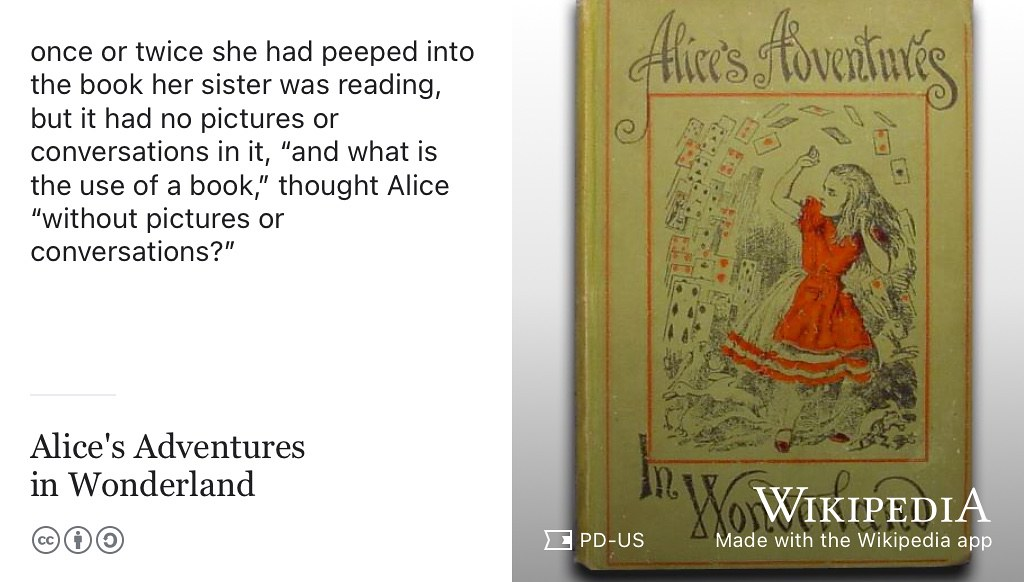
\includegraphics[width=0.99\linewidth]{images/alicequotation} \caption{Alice was beginning to get very tired of sitting by her sister on the bank, and of having nothing to do: once or twice she had peeped into the book her sister was reading, but it had no pictures or conversations in it, ``and what is the use of a book,'' thought Alice ``without pictures or conversations? \citep{wonderland} Public domain image of the cover of the 1898 edition of the novel \emph{\href{https://en.wikipedia.org/wiki/Alice\%27s_Adventures_in_Wonderland}{Alice's Adventures in Wonderland}} via Wikimedia Commons \href{https://w.wiki/3S4C}{w.wiki/3S4C} adapted using the \href{https://apps.apple.com/us/app/wikipedia/id324715238}{Wikipedia app}}\label{fig:aiw-fig}
\end{figure}



Pictures explain. Pictures help you understand. Pictures help you imagine. So this book uses pictures (and conversations) to help you imagine and visualise your future.

\hypertarget{vaccine}{%
\section{Your future aims}\label{vaccine}}

This guidebook aims to help you develop stronger habits of mind, body and soul using five key ingredients:

\begin{enumerate}
\def\labelenumi{\arabic{enumi}.}
\tightlist
\item
  \textbf{\texttt{CODE}}: Instructions, algorithms, recipes and strategies contained in this guidebook. This \texttt{code} is for your consumption, not for a machine.
\item
  \textbf{\texttt{DATA}}: Facts, statistics, graphs and pictures collected together for your analysis
\item
  \textbf{\texttt{YOU}}: Activities for you to do in addition to reading
\item
  \textbf{\texttt{FUTURES}}: Possible futures for you to think about. Try not to dwell on the past. Think about the future. Think about \emph{your} future. \citep{thinkaboutthefuture, wroteforluck}
\item
  \textbf{\texttt{ME}}: Hello, my name is Duncan. I'm your tour guide here. If you're feeling a bit lost, follow me.
\end{enumerate}

\begin{figure}

{\centering 
\includegraphics[width=0.69\linewidth]{images/Hello-my-name-is-Duncan} 

}

\caption{Hello my name is \href{https://en.wikipedia.org/wiki/Duncan_(given_name)}{Duncan}. If you're feeling a bit lost, follow me. Image adapted from \emph{Hello my name is \ldots{} sticker} by Eviatar Bach, public domain \href{https://w.wiki/32RV}{w.wiki/32RV}}\label{fig:hello-my-name-fig}
\end{figure}



Coding your future explores techniques for making career decisions, job searching, submitting applications and competing successfully in interviews and the workplace.

Alongside these practical engineering issues, this guidebook also encourages you to \emph{design your future} by taking a step back and reflecting on the bigger picture. You will apply \href{https://en.wikipedia.org/wiki/Computational_thinking}{computational thinking} techniques, to reflect on who you are, what your story is, how you communicate with other people and what your experience is. As there is a computational theme, you will also need to reflect on what your inputs and outputs (\href{https://en.wikipedia.org/wiki/Input/output}{I/O}) are, both now and in the future. You'll also need to think about what recipes (or algorithms) you might start experimenting with

This guidebook tackles professional issues in computing, for those with and without Computer Science degrees in the early stage of their careers.

\hypertarget{nilo}{%
\section{What you won't learn}\label{nilo}}

This guidebook will NOT teach you how to write code, there's already lots of fantastic resources to help you do that. We discuss some of them in chapter \ref{computing} on \emph{computing your future}.

\hypertarget{bilo}{%
\section{Learning your future}\label{bilo}}

So what \emph{will} you learn from this guidebook? After reading this guidebook, watching the videos and doing the exercises you will be able to:

\begin{enumerate}
\def\labelenumi{\arabic{enumi}.}
\tightlist
\item
  Improve your self-awareness by describing who you are, what motivates you and your strengths and weaknesses
\item
  Decide on a job search strategy and identify employers, sectors and roles that are of interest to you\\
\item
  Improve your written communication skills both for job applications and communicating with other people
\item
  Plan and prepare competitive written applications using standard techniques including CVs, covering letters, application forms and digital profiles
\item
  Compete successfully in interviews and assessment centres by preparing for technical and non-technical questions
\item
  Plan further steps in your career such as promotion, postgraduate study \& research, alternative employment and longer term goals
\item
  Search and navigate a large ``wordbase'' (this guidebook and the work it cites). A wordbase is like a \href{https://en.wikipedia.org/wiki/Codebase}{\texttt{codebase}}, only written predominantly in natural language.
\end{enumerate}

\hypertarget{prereq}{%
\subsection{Your future requirements}\label{prereq}}

As the title of this guidebook implies, there is a computational flavour here, but you do not have to be studying Computer Science to benefit. There are two main target audiences for this guidebook:

\begin{enumerate}
\def\labelenumi{\arabic{enumi}.}
\tightlist
\item
  Undergraduate and postgraduate students studying Computer Science as a major or minor part of their degree. This includes software engineering, artificial intelligence, human-computer interaction (HCI), information systems, health informatics, data science, gaming, cybersecurity and all the other myriad flavours of Computer Science
\item
  Undergraduate and postgraduate students studying \emph{any} subject, with little or no Computer Science at all. You are curious to know about what role computing could play in your future career because computing is too important to be left to Computer Scientists, see chapter \ref{computing} on \emph{Computing your Future}
\end{enumerate}

So the prerequisites for this book are that you are studying (or have studied) at University where English is one of the main spoken languages. You \emph{may} have some experience already, either casual, voluntary or otherwise, but this book does \textbf{not} assume that you have already been employed in some capacity.

\hypertarget{gut}{%
\subsection{Gutting your future}\label{gut}}

Reading this book from cover to cover like a novel is not recommended. That would be foolish.

\begin{figure}

{\centering 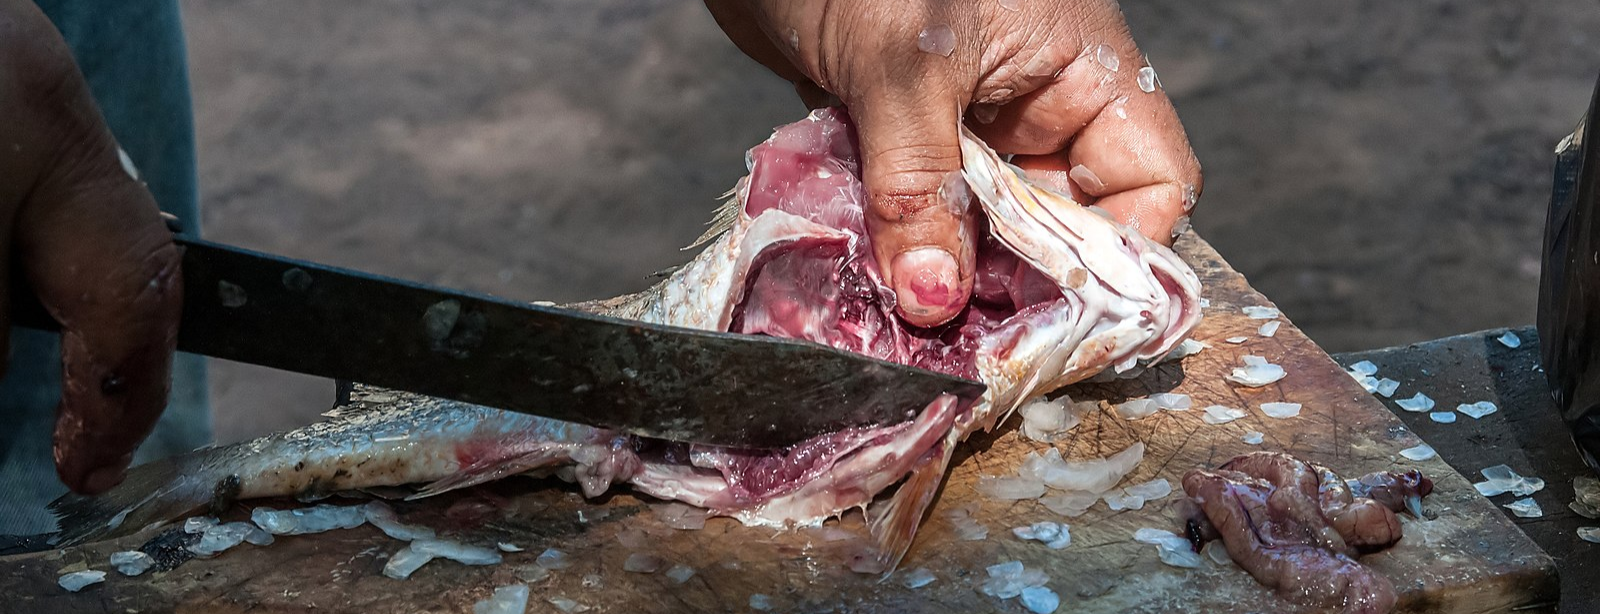
\includegraphics[width=1\linewidth]{images/fish-gutting} 

}

\caption{Don't \emph{read} this book, \href{https://en.wikipedia.org/wiki/Disembowelment}{disembowel it}! Eviscerate it! Gut it like a fish! Enjoy the nourishing flesh and discard the less appetising organs of its gastrointestinal tract. You'll need to decide which is which, depending on your tastes and appetite. CC0 Public domain image of fish gutting by Wilfredor via Wikimedia commons \href{https://w.wiki/_23m}{w.wiki/\_23m} adapted using the \href{https://apps.apple.com/gb/app/wikipedia/id324715238}{Wikipedia app}}\label{fig:gut-fig}
\end{figure}



Instead of reading this book, I suggest you follow the advice given to historian \href{https://en.wikipedia.org/wiki/William_Woodruff}{William Woodruff} about reading books when he was at University:

\begin{quote}
``You don't READ books, you GUT them!'' \citep{nabend} 🐟
\end{quote}

So, gut this book like the fish in figure \ref{fig:gut-fig}. Identify the chapters that are most useful to you (the flesh), and skip the rest (the guts). Which chapters are flesh and which are guts will depend on what stage of the journey you are at. This guidebook is designed to be as ``guttable'' as possible. To aid gutting, the version published at \href{https://www.cdyf.me/}{cdyf.me} has a built in search and tables of contents. Before you can gut the fish, you'll need an anatomical map shown in figure \ref{fig:map-fig}.

\hypertarget{mapping}{%
\section{Mapping your future}\label{mapping}}

This guidebook is split into three parts. The first part (Chapters \ref{rebooting} to \ref{computing}) is on design while the second part (chapters \ref{debugging} to \ref{researching}) is on building and testing your future shown in the map in figure \ref{fig:map-fig}. The final part is a help section for supporting your future (chapters \ref{ruling} to \ref{reading}). Let's look in a bit more detail at the content of each of the three parts of this guidebook:

\begin{figure}

{\centering 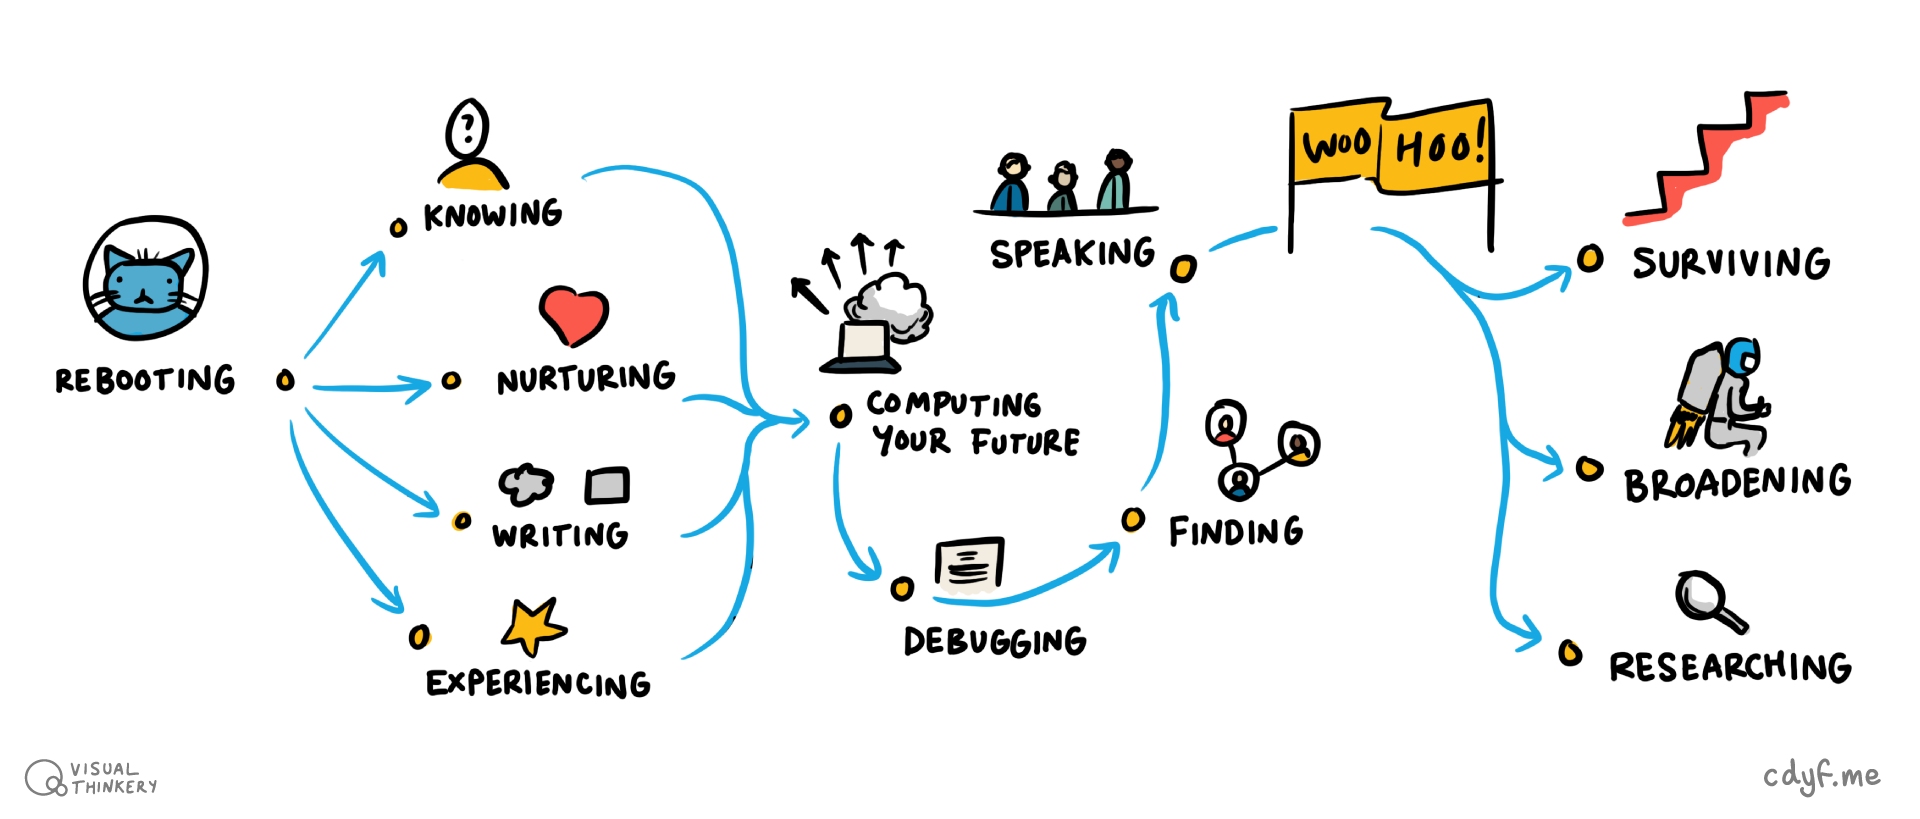
\includegraphics[width=1\linewidth]{images/Course Map V3} 

}

\caption{Mapping your future: Each yellow dot on this diagram is a chapter in \emph{Coding Your Future}. The chapters on the left tackle design issues like \emph{who are you}? Chapters on the right tackle the practicalities of executing and testing your career choices, such as \emph{debugging your CV}. Mapping your Future artwork by \href{https://visualthinkery.com/}{Visual Thinkery} is licenced under \href{https://creativecommons.org/licenses/by-nd/4.0/}{CC-BY-ND}}\label{fig:map-fig}
\end{figure}



\hypertarget{parti}{%
\subsection{Designing your future}\label{parti}}

The first six chapters of this guidebook look at what engineers call \emph{design}. When you build anything, a bridge, a piece of software, a car or a plane you'll need to do some design like the blueprint in figure \ref{fig:brooklyn-fig}

\begin{figure}

{\centering 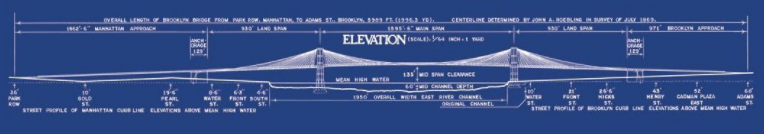
\includegraphics[width=1\linewidth]{images/brooklyn-bridge-blueprint} 

}

\caption{Designing your future is about drawing up a \href{https://en.wikipedia.org/wiki/Blueprint}{blueprint}, like this one for the elevation of the \href{https://en.wikipedia.org/wiki/Brooklyn_Bridge}{Brooklyn Bridge} in New York. What does your blueprint look like? Chapter's \ref{rebooting} through to \ref{computing} will help you design your future.}\label{fig:brooklyn-fig}
\end{figure}



Building a career isn't that different to building anything else, you'll need to do some design work and it will probably be iterative. Designing things often involves asking tricky questions. So when you're designing your future you'll need to cover the following:

\begin{itemize}
\tightlist
\item
  Chapter \ref{rebooting}: \emph{Rebooting your future} discusses why you should bother reading this guidebook
\item
  Chapter \ref{knowing}: \emph{Knowing your future} challenges you to reflect on who you are, what makes you unique and why you are here
\item
  Chapter \ref{nurturing}: \emph{Nurturing your future} encourages you to take care of your mental and physical health
\item
  Chapter \ref{writing}: \emph{Writing your future} explores your soft skills, and how they complement your hard skills and why employers value them so much
\item
  Chapter \ref{experiencing}: \emph{Experiencing your future} asks you to reflect on your work experience and help identify where you can improve it
\item
  Chapter \ref{computing}: \emph{Computing your future} looks at the role computing can play in your career, especially if Computer Science is not a major part of your degree
\end{itemize}

\hypertarget{partii}{%
\subsection{Building your future}\label{partii}}

The next seven chapters look at building (and testing) your future, what engineers like to call \emph{implementation} or \emph{execution} shown in figure \ref{fig:manhattan-fig}.

\begin{figure}

{\centering 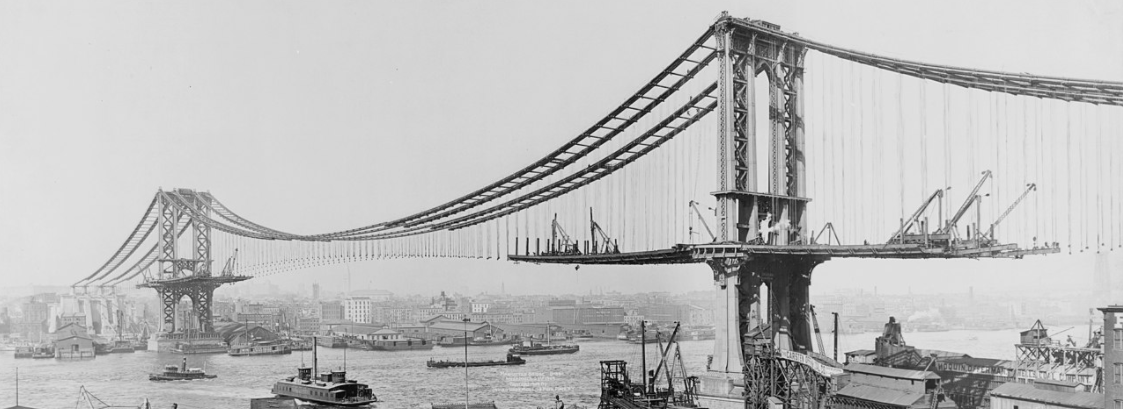
\includegraphics[width=1\linewidth]{images/manhattan_bridge} 

}

\caption{Just like the \href{https://en.wikipedia.org/wiki/Manhattan_Bridge}{Manhattan Bridge}, your future will be easier to build once you've done some design. You don't need a grand design with tonnes of details, a simple sketch will do. Design questions are covered in the first part of this guidebook on designing your future. Picture of the Manhattan bridge under construction in 1909 adapted from a public domain image via Wikimedia commons \href{https://w.wiki/32Rg}{w.wiki/32Rg}}\label{fig:manhattan-fig}
\end{figure}



Once you've started to answer the design questions in the first part, you can start to implement (or build) your career and think about what the next steps will be.

\begin{itemize}
\tightlist
\item
  Chapter \ref{debugging}: \emph{Debugging your future} looks at debugging your written communication such as covering letters, application forms and digital portfolios.
\item
  Chapter \ref{finding}: \emph{Finding your future} looks at where and how can you look for interesting opportunities
\item
  Chapter \ref{broadening}: \emph{Broadening your future} encourages you to broaden your horizons. What are the possibilities beyond the obvious?
\item
  Chapter \ref{speaking}: \emph{Speaking your future} looks how can you turn interviews to your advantage and negotiate any offers you receive
\item
  Chapter \ref{surviving}: \emph{Surviving your future} looks at the next steps. Once you've landed a job, how will you survive and thrive outside (and after) University
\item
  Chapter \ref{achieving}: \emph{Achieving your future} looks at evidence you can collect of your learning and development using various kinds of certifiable evidence
\item
  Chapter \ref{researching}: \emph{Researching your future} discusses if a Masters degree or a PhD right for you?
\end{itemize}

\hypertarget{partiii}{%
\subsection{Supporting your future}\label{partiii}}

The third part of this book, contains supporting material that will help the design, build and test phases described above. You'll need good support to help with the stresses and strains of building your future as shown in \ref{fig:clifton-fig}

\begin{figure}

{\centering 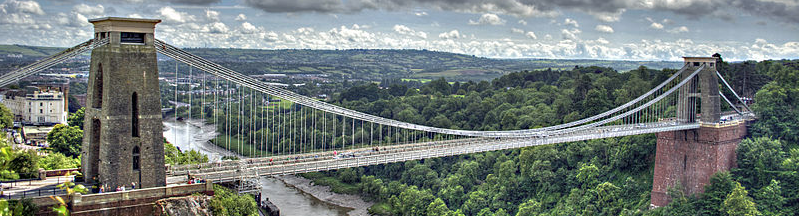
\includegraphics[width=1\linewidth]{images/clifton} 

}

\caption{Huge supporting chains on the \href{https://en.wikipedia.org/wiki/Clifton_Suspension_Bridge}{Clifton Suspension Bridge} in Bristol allow heavy loads pass over the Avon valley bridge. You'll need good support to cope with the stresses and strains of building your future. Clifton suspension bridge picture adapted from original by Nic Trott via Wikimedia commons \href{https://w.wiki/32tu}{w.wiki/32tu}}\label{fig:clifton-fig}
\end{figure}



\begin{itemize}
\tightlist
\item
  Chapter \ref{ruling}: \emph{Ruling your future} provides \emph{Ten Simple Rules for Coding your Future}, this book in a nutshell
\item
  Chapter \ref{hacking}: \emph{Hacking your future} invites you to put yourself in the employers shoes by hacking other people's CVs
\item
  Chapter \ref{moving}: \emph{Moving your future} looks at opportunities outside of capital cities like London
\item
  Chapter \ref{hearing}: \emph{Hearing your future} invites you to listen to students stories of their transition from education to employment
\item
  Chapter \ref{actioning}: \emph{Actioning your future} gets you to think about your actions by emphasising verbs on your job applications
\item
  Chapter \ref{scheduling}: \emph{Scheduling your future} is the live synchronous sessions for this course, if you're not participating in these, schedule a time every day or week for personal development
\item
  Chapter \ref{reading}: \emph{Reading your future} lists everything cited in this guidebook.
\end{itemize}

\hypertarget{themes}{%
\section{Your future themes}\label{themes}}

This guidebook aims to help you build a bridge from where you are now to where you'd like to be in the future. Each chapter of the book contains the following recurring themes:

\begin{figure}

{\centering 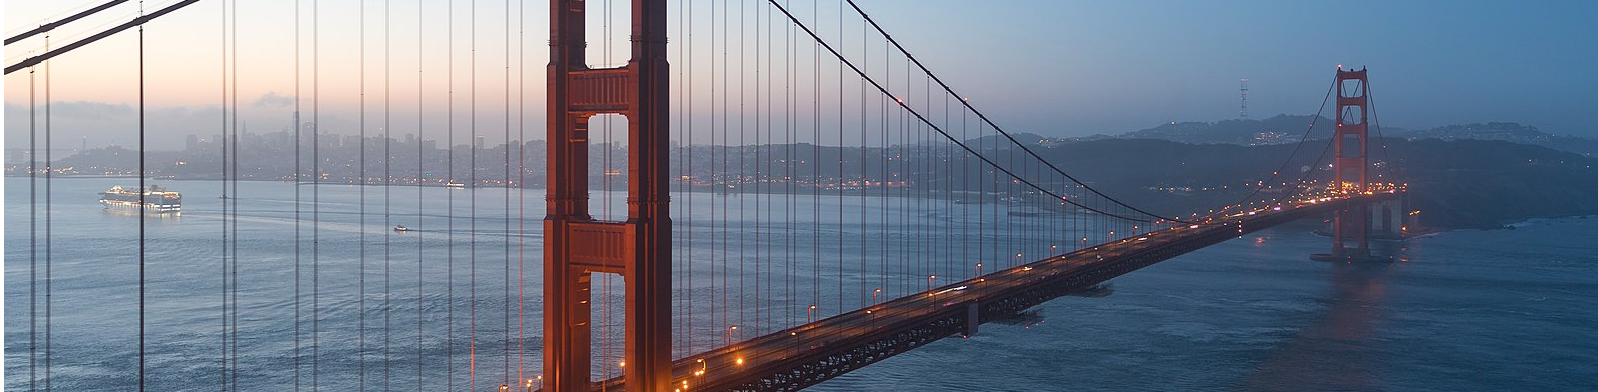
\includegraphics[width=1\linewidth]{images/goldengate} 

}

\caption{This guidebook will help you build a bridge to your future. Picture of the iconic \href{https://en.wikipedia.org/wiki/Golden_Gate_Bridge}{Golden Gate Bridge} in California during the \href{https://en.wikipedia.org/wiki/Blue_hour}{blue hour} adapted from an original by Frank Schulenburg (CC BY-SA) on Wikimedia Commons \href{https://w.wiki/37kY}{w.wiki/37kY}}\label{fig:goldengate-fig}
\end{figure}



\begin{enumerate}
\def\labelenumi{\arabic{enumi}.}
\tightlist
\item
  \textbf{Learning} your future: What you will learn from any given chapter
\item
  \textbf{Watching} your future: videos and animations for you to watch
\item
  \textbf{Listening} to your future: audio and podcasts for you to listen to
\item
  \textbf{Speaking} your future: articulating from a script or by improvisation, particularly when preparing for interviews
\item
  \textbf{Discussing} your future: \href{https://en.wikipedia.org/wiki/Breakpoint}{breakpoints} invite you to pause your code and think about the variables and parameters you are using. Can they be improved? Reflect and discuss.
\item
  \textbf{Reading} your future: reading stuff because its good for your mind, body and soul. Read The Friendly Manual. \href{https://en.wikipedia.org/wiki/RTFM}{\texttt{RTFM}}. Read THIS Friendly Manual.
\item
  \textbf{Writing} your future: written exercises using natural language
\item
  \textbf{Quizzing} your future: quick quizzes to be done in real-time live scheduled sessions described in chapter \ref{scheduling} (synchronously) and in your own time (asynchronously)
\item
  \textbf{Assessing} your future: activities to be assessed by yourself, your peers, an employer or an academic (depending on who and where you are)
\item
  \textbf{Challenging} your future: coding challenges are designed to take you out of your comfort zone by encouraging you to experiment with your thoughts, discussions and actions
\item
  \textbf{Signposting} your future: the most useful resources that I recommend you read, listen to or watch
\end{enumerate}

\hypertarget{contributing}{%
\section{Contributing to your future}\label{contributing}}

If you'd like to contribute this guidebook, I welcome constructive feedback from \href{https://en.wikipedia.org/wiki/Critical_friend}{critical friends}, see figure \ref{fig:critical-friend-fig}. All contributions will be gratefully acknowledged section \ref{thanks} unless you ask for your contributions to remain anonymous.

\begin{figure}

{\centering 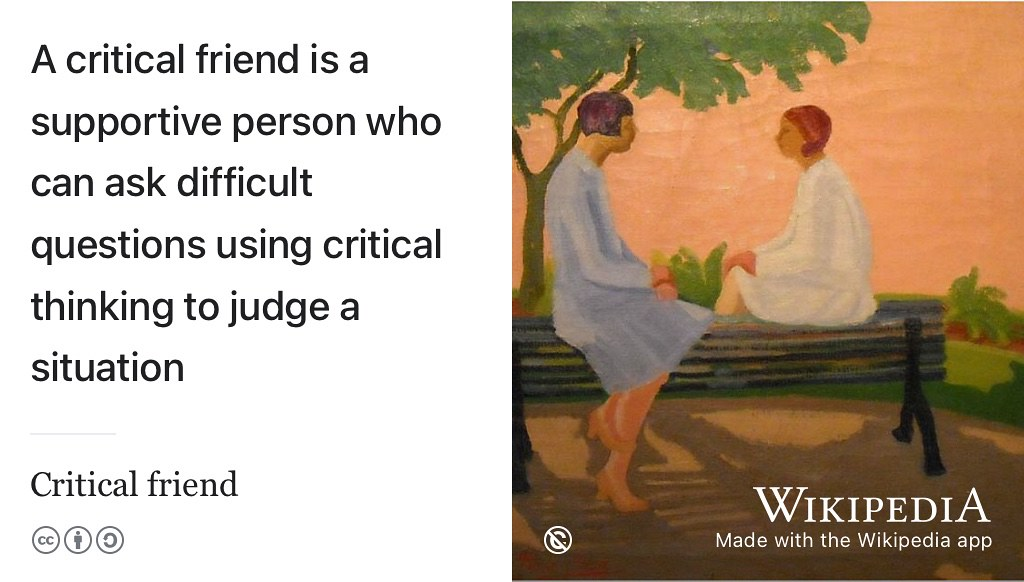
\includegraphics[width=1\linewidth]{images/critical-friend} 

}

\caption{Can you be a supportive but \href{https://en.wikipedia.org/wiki/Critical_friend}{critical friend} of this guidebook? Public domain image of a painting \emph{Friendship} by \href{https://en.wikipedia.org/wiki/Petrona_Viera}{Petrona Viera} via Wikimedia Commons \href{https://w.wiki/3WjY}{w.wiki/3WjY} adapted using the \href{https://apps.apple.com/us/app/wikipedia/id324715238}{Wikipedia App}}\label{fig:critical-friend-fig}
\end{figure}



I'm looking for feedback and contributions on everything in this guidebook from the small things like typos, grammatical errors and spelling mistakes through to bigger issues for each chapter such as:

\begin{itemize}
\tightlist
\item
  Does the chapter make sense, is it clear?
\item
  Does it strike the right tone, is it pitched at the right level? Not patronising? Too many platitudes?
\item
  Are there too many motivational (or \href{https://despair.com/collections/demotivators}{demotivational}) quotations?
\item
  Where is it too long and waffly (see figure \ref{fig:shorterletter-fig}) or too short?
\item
  Are there too many (or too few) pictures? What needs more illustration?
\item
  Is it well scoped? Too broad or too narrow?
\item
  Are the stated learning objectives met by the chapter?
\item
  Are the activities clear? Can students understand why the activities are recommended? What other activities could be added?
\item
  Will it make sense to global readers e.g.~will students from China and India understand the quirks and idioms of English language and culture
\item
  Are there too many metaphors? Mixed metaphors? Awkward analogies? Idiotic idioms? Annoying alliterations?
\item
  Too many citations? Not enough citations? Missed any key citations?
\item
  What's missing?
\item
  Where are the unstated assumptions? Where is the unconscious bias?
\item
  What are the issues with equality, diversity and inclusion?
\item
  Are there too many musical references or annoying emoji? Please bear in mind I'm trying to strike an irreverent, light-hearted and playful tone to improve readability 😜
\item
  What else should be ruthlessly edited out?
\end{itemize}

All suggestions welcome! Don't be shy. There are several ways you can contribute, depending on how comfortable you are with Git:

\hypertarget{techies}{%
\subsection{For git contributors}\label{techies}}

If you're familiar with \texttt{git} and \texttt{markdown} you can \href{https://github.com/join}{github.com/join} and:

\begin{itemize}
\tightlist
\item
  Raise new issues at \href{https://github.com/dullhunk/cdyf/issues/new}{github.com/dullhunk/cdyf/issues/new}
\item
  Click on the \texttt{Edit\ this\ page} link, which appears on the bottom right hand side of every page published at \href{https://www.cdyf.me}{cdyf.me} when viewed with a reasonably large screen (not a phone)
\item
  Contribute at \href{https://github.com/dullhunk/cdyf/contribute}{github.com/dullhunk/cdyf/contribute} and help with existing issues at \href{https://github.com/dullhunk/cdyf/issues}{github.com/dullhunk/cdyf/issues}
\item
  Fork the repository, make changes and submit a pull request \href{https://github.com/dullhunk/cdyf/pulls}{github.com/dullhunk/cdyf/pulls}. If you need to brush-up on your pulling skills see \href{http://makeapullrequest.com/}{makeapullrequest.com}
\item
  From the command line, clone the repository and submit pull requests from your own setup:
\end{itemize}

\begin{Shaded}
\begin{Highlighting}[]
\NormalTok{git clone https://github.com/dullhunk/cdyf.git}
\end{Highlighting}
\end{Shaded}

Most of the guidebook is generated from \href{https://en.wikipedia.org/wiki/Markdown}{RMarkdown}, that's \href{https://github.com/dullhunk/cdyf/search?l=RMarkdown}{all the \texttt{*.Rmd} files}. So markdown files are the only ones you should edit because everything else is generated from them including the \texttt{*.html}, \texttt{*.tex}, \texttt{*.pdf},\texttt{*.epub} and \texttt{*.docx} files.

\hypertarget{elseif}{%
\subsection{For everyone else}\label{elseif}}

If you don't want to (or can't) use Git and \href{https://github.com/}{github.com} then you can:

\begin{itemize}
\tightlist
\item
  Add comments by annotating \href{https://www.cdyf.me/cdyf.pdf}{cdyf.pdf} using your personal weapon of choice (tablet, \href{https://en.wikipedia.org/wiki/ReMarkable}{reMarkable} or whatever) and \href{http://www.cs.man.ac.uk/~hulld/contact.html}{emailing your updated version to me}
\item
  Add comments by annotating \href{https://www.cdyf.me/cdyf.epub}{cdyf.epub} and \href{http://www.cs.man.ac.uk/~hulld/contact.html}{emailing your updated version to me}
\item
  Suggest changes by editing the Microsoft Word version at \href{http://cdyf.me/cdyf.docx}{cdyf.docx}. The text is all there, but the images are all over the place. This is because the pagination, typesetting and graphic placement algorithms in Word aren't anything like as good as the LaTeX ones used to create the \href{https://www.cdyf.me/cdyf.pdf}{cdyf.pdf} (output) from the \href{https://cdyf.me/cdyf.tex}{cdyf.tex} (input).\footnote{Don't say I didn't warn you!} Make sure you've \href{https://support.microsoft.com/en-us/office/track-changes-in-word-197ba630-0f5f-4a8e-9a77-3712475e806a}{turned on track changes in Word}. Track changes is Microsoft Word's \href{https://en.wikipedia.org/wiki/Killer_feature}{killer feature} that allows your corrections to be easily identified from the original text.
\item
  Just \href{http://www.cs.man.ac.uk/~hulld/contact.html}{email me suggestions for improvements}
\end{itemize}

Any corrections or suggestions will be gratefully received and noted in the acknowledgements section \ref{thanks}, unless you tell me otherwise. I welcome all improvements, big and small.

\hypertarget{thanks}{%
\section{Acknowledgements}\label{thanks}}

The content of this book is based on hundreds of conversations I have had with students of Computer Science, Mathematics, Physics and Engineering, since 2012. It is also based on conversations I've had with many of their employers too.

\textbf{\texttt{\#\ Coding\ Comment}}

This acknowledgements section is long because I try to practice what I preach about the importance of expressing gratitude, see section \ref{lays}. It also serves as a live demonstration of a public \href{https://en.wikipedia.org/wiki/Gratitude_journal}{gratitude journal}. Showing gratitude, both public and private, is a proven technique for improving mental health, see \ref{signposts3}.

If you want to get to the main content of this book you can skip this and go straight to chapter \ref{rebooting}.

\hypertarget{students}{%
\subsection{Thank you students}\label{students}}

First and foremost, I would like to thank all the students who have helped with this book, both directly and indirectly see figure \ref{fig:giants-fig}.

\begin{figure}

{\centering 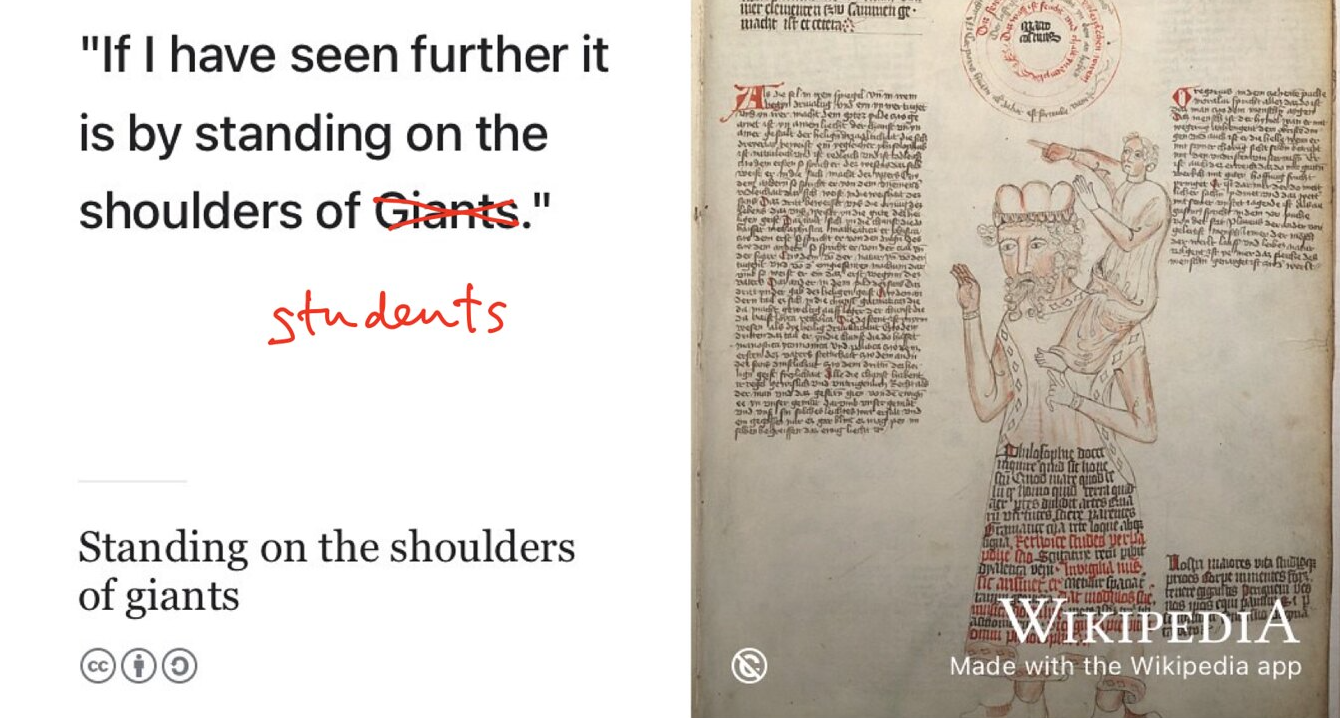
\includegraphics[width=1\linewidth]{images/standing-on-the-shoulders-of-students} 

}

\caption{If I have seen further it is by \href{https://en.wikipedia.org/wiki/Standing_on_the_shoulders_of_giants}{standing on the shoulders of \sout{giants} students}. \citep{newton} Public domain image of \href{https://en.wikipedia.org/wiki/Orion_(mythology)}{Orion} carrying his servant \href{https://en.wikipedia.org/wiki/Cedalion}{Cedalion} on his shoulders via Wikimedia Commons \href{https://w.wiki/_zZ2E}{w.wiki/\_zZ2E}}\label{fig:giants-fig}
\end{figure}



So, if you have studied some flavour of Computer Science at the University of Manchester since 2012, there's a high probability you have contributed to this book. Thank you for having the courage to tell me your stories. Thank you for being ambitious, hard working, talented, fearless, creative, inspirational and listening to me (sometimes). It has been my pleasure and privilege to work with you all.

I'd especially like to thank industrial experience (IE) students who have completed a year in industry as part of their degree as well as those who have done summer internships, either as part of the Master of Engineering (MEng) program or otherwise, particularly \href{https://github.com/samialabed}{Sami Alabed}, Luke Beamish, Eirik Björnerstedt, Petia Davidova and Kristina Radinova. In addition, the \href{http://www.pass.manchester.ac.uk}{PASS leaders} and facilitators, \href{https://unicsmcr.com/}{UniCSmcr.com}, \href{https://github.com/unicsmcr/hacksoc.com}{HackSoc}, \href{https://github.com/cssoc}{CSSoc} and \href{https://github.com/Man-UP}{Manchester Ultimate Programming} members have all been influential on the content of this book. I've learned heaps by manually trawling through thousands of your CVs too, so if you've shown me a copy of your CV, thanks! If you sent me a CV and I didn't reply, I apologise. There are limits to what is humanly possible. Chapter \ref{debugging} on \emph{Debugging your future} (self assessment) and chapter \ref{hacking} on \emph{Hacking your future} (peer assessment) are based on the most common bugs (or are they features?) I've seen in CVs.

\begin{figure}

{\centering \includegraphics[width=1\linewidth]{images/bbcbreakfastsofa} 

}

\caption{Posing on the \href{https://en.wikipedia.org/wiki/BBC_Breakfast}{BBC Breakfast} red sofa with the winning student team at the BBC / Barclays University Technology Challenge (UTC) in \href{https://en.wikipedia.org/wiki/MediaCityUK}{MediaCityUK}, Salford, Greater Manchester}\label{fig:unnamed-chunk-3}
\end{figure}



So, thank you students for being studious. 🙏

\hypertarget{employers}{%
\subsection{Thank you employers}\label{employers}}

Thanks to all the organisations who have employed students from the Department of Computer Science as either summer interns, year long placements or graduates. A big chunk of this guidebook documents their experience of employers and their graduate recruitment programs.

Thanks to Niall Beard and \href{https://github.com/sharifsalah}{Sharif Salah} at Google for introducing me to Google's Technical Writing course. \citep{googling}

So, thanks employers for employing our students. 🙏

\hypertarget{colleagues}{%
\subsection{Thank you colleagues}\label{colleagues}}

I've also had significant support from colleagues in the Department of Computer Science (\href{https://twitter.com/csmcr}{@csmcr}) and support staff at the University of Manchester. (\href{https://twitter.com/UoMCareers}{@UoMCareers}, \href{https://twitter.com/alumniUoM}{@alumniUoM}, \href{https://twitter.com/OfficialUoM}{@OfficialUoM})

I would especially like to thank \href{https://en.wikipedia.org/wiki/James_John_Miles}{Jim Miles} for encouraging me to write a book shortly after he offered me a job. I thought he was joking (about the book) but it actually turned out to be another one of Jim's great ideas. Thanks Jim. 🙏

I'd also like to thank the only three people in the whole world who've had the misfortune of reading all of my PhD thesis; \href{https://en.wikipedia.org/wiki/Robert_David_Stevens}{Robert Stevens}, \href{https://www.ncl.ac.uk/computing/staff/profile/anilwipat.html}{Anil Wipat} and \href{https://en.wikipedia.org/wiki/Steve_Pettifer}{Steve Pettifer}. I suspect it was as painful for you to read as it was for me to write it. Thanks Robert for your relentless patience and giving me a well timed, well aimed kick up the (proverbial) arse to write this book in the \href{https://en.wikipedia.org/wiki/Midland_Hotel,_Manchester}{Midland Hotel, Manchester} at the May ball.

Thanks \href{https://en.wikipedia.org/wiki/Steve_Furber}{Steve Furber} for playing bass guitar in our ``boy band'' \href{http://www.cs.man.ac.uk/~hulld/research.html\#tuningcomplete}{Tuning Complete}. Thanks to \href{https://en.wikipedia.org/wiki/Carole_Goble}{Carole Goble} for patiently re-teaching me how to write by covering early drafts of my MSc thesis in red ink and less patiently (on subsequent revisions) swear words. 🤬

So, thank you colleagues for being collegiate. You make the University of Manchester an enjoyable place to work.

\hypertarget{academia}{%
\subsubsection{Thanks to academic staff}\label{academia}}

Thanks to past and present academic colleagues (see figure \ref{fig:academics-fig}), PhD students and teachers at the University of Manchester (and elsewhere) who have contributed to this guidebook and the environment it was written in. We are bound together by the power of weak ties (section \ref{weakties}) alongside stronger forces and friendships.

\begin{figure}

{\centering 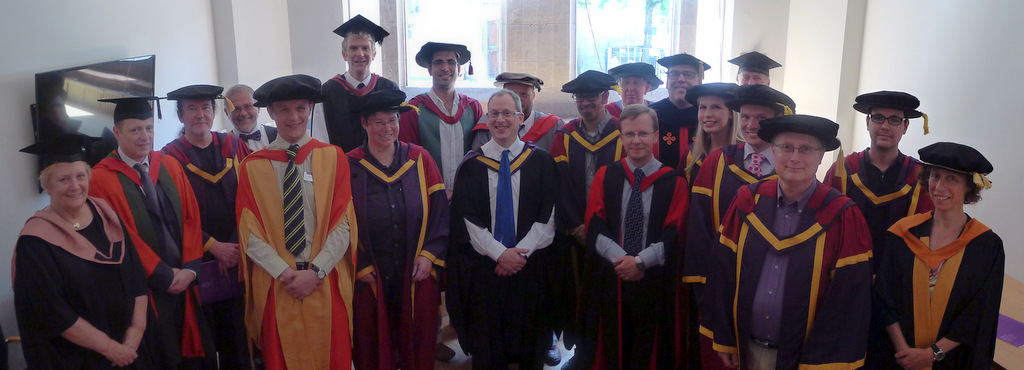
\includegraphics[width=1\linewidth]{images/graduation-ceremony-2013} 

}

\caption{Wearing silly hats and even sillier frocks for a graduation ceremony in the \href{https://en.wikipedia.org/wiki/Whitworth_Hall}{Whitworth Hall}, Manchester in 2013. From left to right Alex Walker, Tim Morris, John Latham, Graham Gough, Yours Truly, Sean Bechhofer, Andrea Schalk, Gavin Brown, Toby Howard, Robert Stevens, Simon Harper, Barry Cheetham, Norman Paton, Bijan Parsia, Caroline Jay, Allan Ramsay, Darren Lunn, Nick Filer, Markel Vigo and Ulrike Sattler. Picture by Toby Howard. 🎓}\label{fig:academics-fig}
\end{figure}



They include (in alphabetical order): Muideen Ajagbe, Pinar Alper, Sophia Ananiadou, Mikel Egaña Aranguren, Constantinos Astreos, Terri Attwood, Sam Bail, \href{https://en.wikipedia.org/wiki/Robin_Baker_(biologist)}{Robin Baker}, Richard Banach, Riza Batista-Navarro, Michael Bada, Niall Beard, Sean Bechhofer, Casey Bergman, Lynne Bianchi, Ahmad Bilal, Helena Björn van Praagh, Stewart Blakeway, Petrut Bogdan, Caroline Bowsher, Linda Brackenbury, Andy Brass, Judy Brewer, Christian Brenninkmeijer, Andy Bridge, Andy Brown, Gavin Brown, Nick Brown, Mihai Bujanca, Zhongyan Chen, Oscar Corcho, Terry V. Callaghan, Grant Campbell, Angelo Cangelosi, Peter Capon, Andy Carpenter, Nicola Carrier, Thomas Carroll, Barry Cheetham, Ke Chen, Sarah Clinch, Ian Cottam, Brian Cox, Simone Di Cola, Paul Dobson, Clare Dixon, Danny Dresner, Nick Drummond, Warwick Dunn, Dominic Duxbury, Doug Edwards, Iliada Eleftheriou, Anas Elhag, Suzanne Embury, \href{https://www.uoguelph.ca/mcb/people/dr-michael-j-emes}{Michael Emes}, Alvaro Fernandes, Jonathan Ferns, Michele Filannino, Nick Filer, Paul Fisher, Steve Furber, Andre Freitas, Aphrodite Galata, Matthew Gamble, Jim Garside, Kristian Garza, Chris Gilbert, Danielle George, Richard Giordano, Birte Glimm, Carole Goble, Rafael Gonçalves, Antoon Goderis, Roy Goodacre, Graham Gough, Bernardo Cuenca Grau, Peter R. Green, \href{https://en.wikipedia.org/wiki/Keith_Gull}{Keith Gull}, John Gurd, Luke Hakes, Robert Haines, Guy Hanke, Simon Harper, Jonathan Heathcote, \href{https://github.com/eldog}{Lloyd Henning}, Gareth Henshall, Andrew Horn, Farid Kahn, Chris Hardacre, Matthew Horridge, Ian Horrocks, Toby Howard, Roger Hubbold, Luigi Iannone, Jane Ilsley, Jules Irenge, Daniel Jameson, Caroline Jay, Mirantha Jayathilaka, Huw Jones, Simon Jupp, Yevgeny Kazakov, John Keane, Douglas Kell, Catriona Kennedy, Rachel Kenyon, Chris Knight, Joshua Knowles, Dirk Koch, Nikolaos Konstantinou, Christos Kotselidis, Ioannis Kotsiopoulos, Oliver Kutz, Alice Larkin, Peter Lammich, John Latham, Kung-Kiu Lau, Hugo Lefeuvre, Dave Lester, Peter Li, Zewen Liu, Phil Lord, Mikel Luján and Darren Lunn\ldots{} (continued after the gratuitous picture break of figure \ref{fig:msc-fig})

\begin{figure}

{\centering 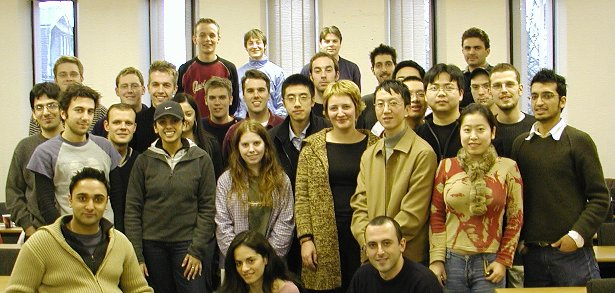
\includegraphics[width=1\linewidth]{images/msc-2003} 

}

\caption{Masters and Mistresses of Science, part of the \href{https://web.archive.org/web/20030825205716/http://www.cs.man.ac.uk/Study_subweb/Postgrad/ACS-CS/webpages/handbook/CSHandbook.pdf}{MSc Computer Science} class of 2003. \href{https://en.wikipedia.org/wiki/Where\%27s_Wally\%3F}{Where's Wally?} You should be able to find me although I'm \emph{not} wearing a red and white stripy jumper. Picture by \href{https://www.southampton.ac.uk/healthsciences/about/staff/richard_giordano.page}{Richard Giordano}.}\label{fig:msc-fig}
\end{figure}



\ldots{} (continued) Matthew Makin, Nicolas Matentzoglu, Paul Mativenga, Erica McAlister, Mary McGee Wood, April McMahon, Merc and members of the \href{https://www.mumc.me.uk/wordpress}{Manchester University Mountaineering Club} (MUMC), Simon Merrywest, Eleni Mikroyannidi, Colin Morris, Norman Morrison, Georgina Moulton, Boris Motik, Christoforos Moutafis, Tingting Mu, Ettore Murabito, Mustafa Mustafa, Javier Navaridas, Kostas Nikolou, Aleksandra Nenadic, Goran Nenadic, Steve McDermott, Jock McNaught, Mary McGee-Wood, Pedro Mendes, Sarah Mohammad-Qureshi, Tim Morris, Jennifer O'Brien, Tim O'Brien, Steve Oliver, Pierre Olivier, Mario Ramirez Orihuela, Stuart Owen, Ali Owrak, Liam Panchaud, Pavlos Petoumenos, David Petrescu, Luis Plana, \href{https://www.brookes.ac.uk/ocsld/about-ocsld/staff-profiles/jackie-potter/}{Jackie Potter}, \href{https://en.wikipedia.org/wiki/Malcolm_Press}{Malcolm Press}, Colin Puleston, Paul Nutter, Ignazio Palmisano, Dario Panada, Michael Parkin, Bijan Parsia, Jon Parkinson, Norman Paton, Jeff Pepper, Steve Pettifer, Rishi Ramgolam, Allan Ramsay, Magnus Rattray, Alasdair Rawsthorne, Farshid Rayhan, Alan Rector, Giles Reger, Graham Riley, David Robertson, Jeremy Rodgers, Clare Roebuck, Mauricio Jacobo Romero, Nancy Rothwell, William Rowe, Oliver Rhodes, David Rydeheard, Graham Riley, Daniella Ryding, Ulrike Sattler, Ahmed Saeed, Pejman Saeghe, Rizos Sakellariou, Pedro Sampaio, Sandra Sampaio, John Sargeant, Andrea Schalk, Viktor Schlegel, Renate Schmidt, Jonathan Shapiro, \href{https://www.manchester.ac.uk/discover/governance/structure/board-governors/members/liz-sheffield/}{Liz Sheffield}, Bushra Sikander, Lemn Sissay, Vangelis Simeonidis, Kieran Smallbone, Alastair Smith, Stian Soiland-Reyes, Irena Spasic, David Spendlove, Robert Stevens, Alan Stokes, Shoaib Sufi, James Sumner, \href{https://github.com/dj-foxxy}{Peter Sutton}, Neil Swainston, \href{https://www.springer.com/gp/book/9780412303203}{John H. Tallis}, Paul Taplin, Federico Tavella, Chris Taylor, Tom Thomson, Dave Thorne, David Toluhi, \href{https://www.theguardian.com/science/2020/nov/10/tony-trinci-obituary}{Tony Trinci}, Dimitri Tsarkov, Daniele Turi, Jake Vasilakes, Laura Vasques, Delia Vazquez, Giles Velarde, Chiara Del Vescovo, Markel Vigo, Sam de Visser, Andrei Voronkov, Niels Walet, Alex Walker, Louise Walker, Dieter Wiechart, Igor Wodiany, Katy Wolstencroft, Natalie Wood, Chris Wroe, Crystal Wu, Lisheng Wu, Yifan Xu, Viktor Yarmolenko, Yeliz Yesilada, He Yu, Serafeim Zanikolas, Xiao-Jun Zeng, Jun Zhao, Liping Zhao, Ning Zhang and Evgeny Zolin.

\begin{figure}

{\centering 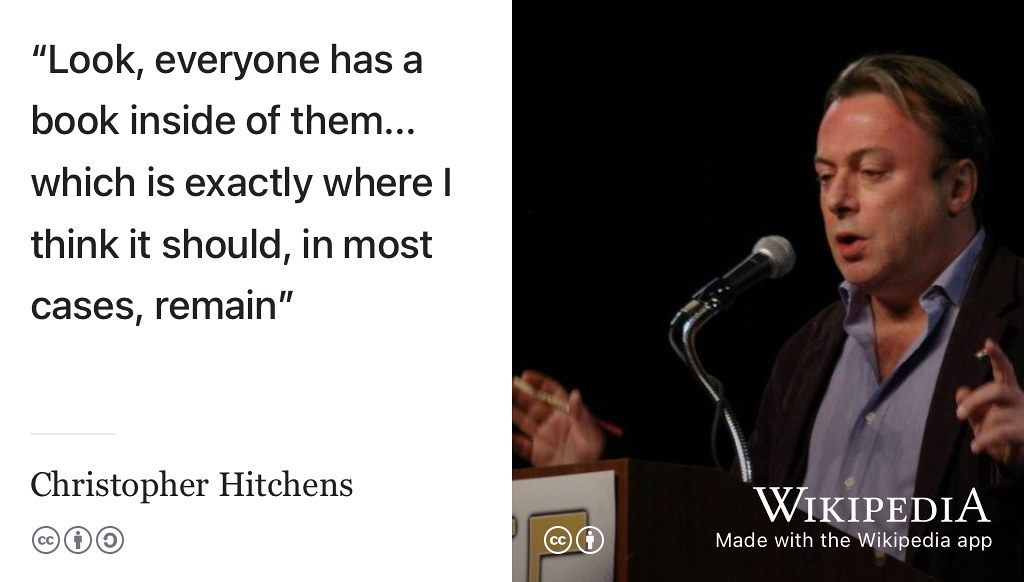
\includegraphics[width=0.99\linewidth]{images/everyone-has-a-book-inside-them} 

}

\caption{Optimists will tell you that ``everyone has a book in them\ldots{}'', but pessimists like \href{https://en.wikipedia.org/wiki/Christopher_Hitchens}{Christopher Hitchens} will add that ``\ldots in most cases that's exactly where it should remain''. \citep{everyone} Despite Hitchens amusing trademark scepticism, I am optimistic about the power of natural languages, written and spoken. CC BY portrait of Christopher Hitchens by ensceptico via Wikimedia Commons \href{https://w.wiki/3YK7}{w.wiki/3YK7} adapted using the \href{https://apps.apple.com/us/app/wikipedia/id324715238}{Wikipedia app}}\label{fig:hitchens-fig}
\end{figure}



So thanks academics for being even more sceptical than Christopher Hitchens, see figure \ref{fig:hitchens-fig}. Thanks academics for being academic. 🙏

\hypertarget{psstaff}{%
\subsubsection{Thank you professional services staff}\label{psstaff}}

Thanks also to the superb support staff (past and present) from professional services, especially the Academic Support Office (ACSO), Student Support Office (SSO) and external affairs office in the Kilburn building. Professional services staff continue to make all the magic of teaching and learning possible: Alyx Adams, Daniele Atkinson, Cassie Barlow, Jennie Ball-Foster, Emma Bentley, Christine Bowers, Karen Butterworth, Chris Connolly, Ellie Crompton, Jean Davison, Gavin Donald, Miriam Cadney, Chris Calland, Ben Carter, Hannah Cousins, Holly Dewsnip, Tammy Goldfeld, Penney Gordon-Lanes, Amelia Graham, Iain Hart, Kath Hopkins, Lynn Howarth, Yvonne Hung, Susie Hymas, Radina Ivanova, Dan Jagger, Alex Jones, Jeremy Jones, Jessicca Kateryniuk-Smith, Mike Keeley, Stephanie Lee, Dominic Laing, Gill Lester, Jez Lloyd, Ruth Maddocks, Cameron Macdonald, Tony McDonald, Karon Mee, Anne Milligan, Rachel Mutters, Matthew Oakley, Alyson Owens, Chris Page, Melanie Price, Abby Ragazzon-Smith, Chris Rhodes, Graham Richardson, Martin Ross, Julian Skyrme, Elaine Sheehan, Angela Standish, Martine Storey, Bernard Strutt, Jannine Thomas, Joseph Tirone, Daisy Towers, Anna Warburton-Ball, Richard Ward, Sarah White, Elizabeth Wilkinson, Andrew Whitmore, Lisa Wright and Mabel Yau.

And Wendy. We all miss you and love you Wendy. \href{https://www.justgiving.com/crowdfunding/byte-cafe}{\#JusticeForWendy} ✊🏽 \href{https://en.wikipedia.org/wiki/Fight_the_Power_(Public_Enemy_song)}{Fight the Power}! ✊🏽 \citep{fightthepower}

So, thanks professional services staff for being professional and supporting the work of teaching. 🙏

\hypertarget{sigcse}{%
\subsection{Thank you SIGCSE}\label{sigcse}}

Thanks to the \href{https://www.sigcse.org}{SIGCSE.org}, the Special Interest Group (SIG) on Computer Science Education (CSE), part of the Association for Computing Machinery \href{https://www.acm.org/}{ACM.org}. Thanks to my fellow \href{https://uki-sigcse.acm.org/}{uki-sigcse.acm.org} board members \href{https://www.dur.ac.uk/research/directory/staff/?mode=staff\&id=106}{Steven Bradley}, \href{https://www.kent.ac.uk/computing/people/3101/carter-janet}{Janet Carter}, \href{https://proftomcrick.com/}{Tom Crick}, \href{https://www.gla.ac.uk/schools/computing/staff/quintincutts/}{Quintin Cutts}, \href{https://en.wikipedia.org/wiki/Sally_Fincher}{Sally Fincher}, \href{https://www.advance-he.ac.uk/ntfs/dr-samia-kamal}{Samia Kamal}, \href{https://www.gla.ac.uk/schools/computing/staff/josephmaguire/}{Joseph McGuire} and \href{https://www.napier.ac.uk/people/sally-smith}{Sally Smith} for their help and advice, see figure \ref{fig:sigcse-fig}

\begin{figure}

{\centering 
\includegraphics[width=0.99\linewidth]{images/sigcse} 

}

\caption{Every year in January practitioners and researchers in computing education, both within Computer Science departments and elsewhere gather for \href{https://cepconference.webspace.durham.ac.uk/}{Computing Education Practice} (CEP) in Durham. Come and join our \href{https://uki-sigcse.acm.org/practice/}{vibrant and thriving community}! Picture of \href{https://en.wikipedia.org/wiki/Durham_Cathedral}{Durham Cathedral} by \href{https://commons.wikimedia.org/wiki/User:Mattbuck}{Mattbuck} via Wikimedia Commons \href{https://w.wiki/4acc}{w.wiki/4acc} adapted using the \href{https://apps.apple.com/us/app/wikipedia/id324715238}{Wikipedia app}}\label{fig:sigcse-fig}
\end{figure}



Thanks to all the \href{https://sigcse.cs.manchester.ac.uk}{SIGCSE journal clubbers} including \href{https://www.brettbecker.com/}{Brett Becker}, Ceredig Cattanach-Chell, \href{https://en.wikipedia.org/wiki/James_H._Davenport}{James Davenport}, \href{https://riceacademy.rice.edu/junior-fellows/dr-rodrigo-ferreira}{Rodrigo Ferreira}, \href{https://www.nottingham.ac.uk/computerscience/people/colin.johnson}{Colin Johnson}, \href{https://www.gla.ac.uk/pgrs/nicolalooker/}{Nicola Looker}, Julia Markel, \href{https://www.gcu.ac.uk/cebe/staff/jim\%20paterson/}{Jim Paterson}, \href{https://en.wikipedia.org/wiki/Sue_Sentance}{Sue Sentance}, \href{https://www.brookes.ac.uk/templates/pages/staff.aspx?uid=p0073862}{David Sutton}, \href{https://en.wikipedia.org/wiki/Moshe_Vardi}{Moshe Vardi}, \href{http://eecs.qmul.ac.uk/profiles/waitejanelisa.html}{Jane Waite} and \href{https://www.open.ac.uk/people/mw4687}{Michel Wermelinger}. Many of our journal club conversations have fed directly into the content of this guidebook.

Thanks to Sally Fincher and Janet Finlay whose report \href{https://kar.kent.ac.uk/53848}{Computing Graduate Employability: Sharing Practice} \citep{fincherreview} has had a big influence on this guidebook.

So thanks SIGCSE for being special and interesting. 🙏

\hypertarget{scientists}{%
\subsection{Thank you scientists}\label{scientists}}

There is a wider community of scientists, engineers and scholars that have influenced this guidebook:

\begin{itemize}
\tightlist
\item
  Thanks to \href{https://en.wikipedia.org/wiki/David_J._Malan}{David Malan} (\href{https://cs.harvard.edu/malan/}{@malan}) for \href{https://en.wikipedia.org/wiki/CS50}{CS50} which continues to be an inspiration to me and many others. \citep{cs50, cs50zoom, CS502021} Thanks to \href{https://crisbodnar.github.io/}{Cristian Bodnar} for inviting David to run \href{http://cs50.hacksoc.com}{CS50 in Manchester} in 2017 which was a great introduction to David's work \citep{cs50mcr}
\item
  Thanks to \href{https://en.wikipedia.org/wiki/Laurie_R._Santos}{Laurie Santos} (\href{https://twitter.com/lauriesantos}{@lauriesantos}), for \emph{The Science of Well-being} (TSOWB) \citep{lauriesantos} which was been a significant influence on this book had a gradual but significant effect on my personal and professional life. I've tried to distill some of the ideas into chapter \ref{nurturing} on \emph{Nurturing your future}
\item
  Thanks to \href{https://en.wikipedia.org/wiki/Hadley_Wickham}{Hadley Wickham} (\href{https://github.com/hadley}{@hadley}) and Garrett Grolemund (\href{https://github.com/garrettgman}{@garrettgman}) for \emph{R for Data Science} \citep{r4ds} which helped me get started with R and bookdown. If you're reading this page in some kind of web browser, the stylesheet used here is re-used from \href{https://r4ds.had.co.nz/}{r4ds.had.co.nz}
\item
  Thanks to \href{https://en.wikipedia.org/wiki/Athene_Donald}{Athene Donald} and \href{https://occamstypewriter.org/scurry/}{Stephen Curry} at \href{http://occamstypewriter.org/athenedonald/}{Occams Typewriter} for writing stuff that has informed, entertained and inspired me
\item
  Thanks to \href{https://www.new.ox.ac.uk/node/1003}{Jonathan Black} (\href{https://twitter.com/JonathanPBlack}{@JonathanPBlack}) for his book \emph{Where am I Going, Can I Have a Map?}, his \emph{Financial Times} columns and videos. \citep{jonathanblack, ft}
\item
  Thanks to \href{https://en.wikipedia.org/wiki/David_Alan_Walker}{David Alan Walker} for his book \emph{Energy, Plants \& Man} which inspired the conversations and pictures idea behind this book. \citep{epm}
\end{itemize}

So thanks scientists (and engineers) for being scientific and engineering. 🙏

\hypertarget{bath}{%
\subsection{Thank you Bath}\label{bath}}

As a graduate of the \href{https://en.wikipedia.org/wiki/Postgraduate_Certificate_in_Education}{Postgraduate Certificate in Education} (PGCE) in Science at the \href{https://en.wikipedia.org/wiki/University_of_Bath}{University of Bath} (graduated 2011), I have been heavily influenced by the fantastic work of PGCE science course leaders Caroline Padley (Physics), Steve Cooper (Chemistry), Malcolm Ingram (Biology) and fellow students on the course.

\begin{figure}

{\centering 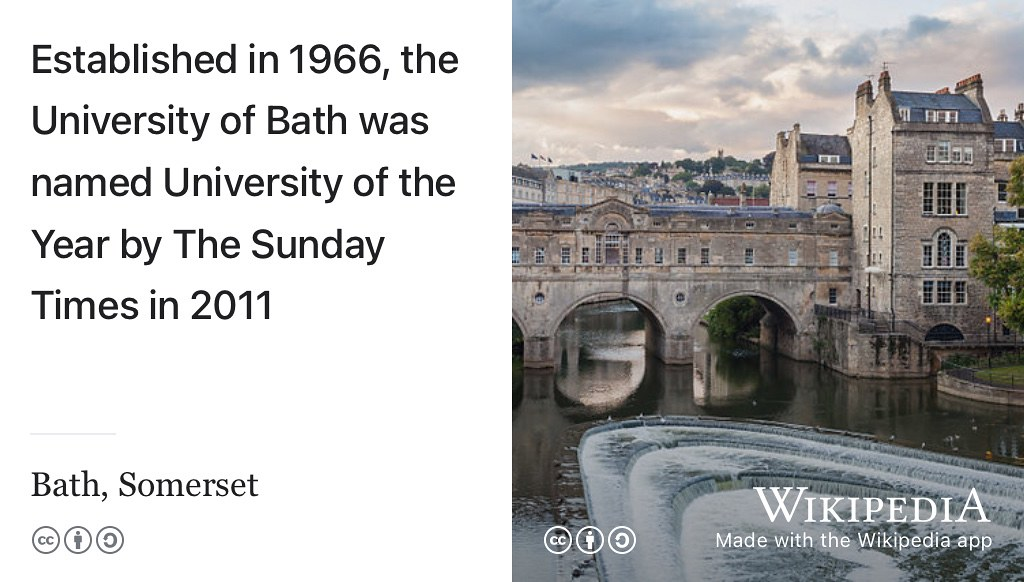
\includegraphics[width=1\linewidth]{images/bath-panorama} 

}

\caption{Named after its \href{https://en.wikipedia.org/wiki/Roman_Baths_(Bath)}{Roman Baths}, the \href{https://en.wikipedia.org/wiki/Bath,_Somerset}{City of Bath} is home to the University of Bath which was named \href{https://en.wikipedia.org/wiki/Sunday_Times_University_of_the_Year}{\emph{Sunday Times} University of the Year} in 2011. Picture of \href{https://en.wikipedia.org/wiki/Pulteney_Bridge}{Pulteney Bridge} by Diego Delso, \href{http://delso.photo/}{delso.photo}, License \href{https://creativecommons.org/licenses/by-sa/4.0/legalcode}{CC-BY-SA} via Wikimedia Commons at \href{https://w.wiki/3VWY}{w.wiki/3VWY} adapted using the Wikipedia app}\label{fig:bath-fig}
\end{figure}



Thanks Bath for the initial teacher training (ITT), the medicinal \href{https://en.wikipedia.org/wiki/Aquae_Sulis}{Aquae Sulis} and the beautiful \href{https://en.wikipedia.org/wiki/Cotswolds}{Cotswolds} Area of Outstanding Natural Beauty (\href{https://en.wikipedia.org/wiki/Area_of_Outstanding_Natural_Beauty}{AONB}). 🙏

\hypertarget{shaftesbury}{%
\subsection{Thank you Shaftesbury}\label{shaftesbury}}

Thanks to Chris Almond, David Ball, David Booth, Caroline Dallimore, Stuart Ferguson, Caroline Moss, Mr Travers and all the other staff and students at \href{https://en.wikipedia.org/wiki/Shaftesbury_School}{Shaftesbury School} who hosted my first PGCE teaching placement, see figure \ref{fig:shaft-fig}. Thanks also to my fellow Shaftesbury and Bath trainees Katharine Platt, Harriet Edwards, Vicky Dury and Joan Shaw for sharing their knowledge through \href{https://en.wikipedia.org/wiki/Peer_learning}{peer learning}. Thanks Joan for keeping me awake on the long and winding west country roads to and from deepest darkest Dorset. Thanks for sharing the heavy burden of driving too.

\begin{figure}

{\centering 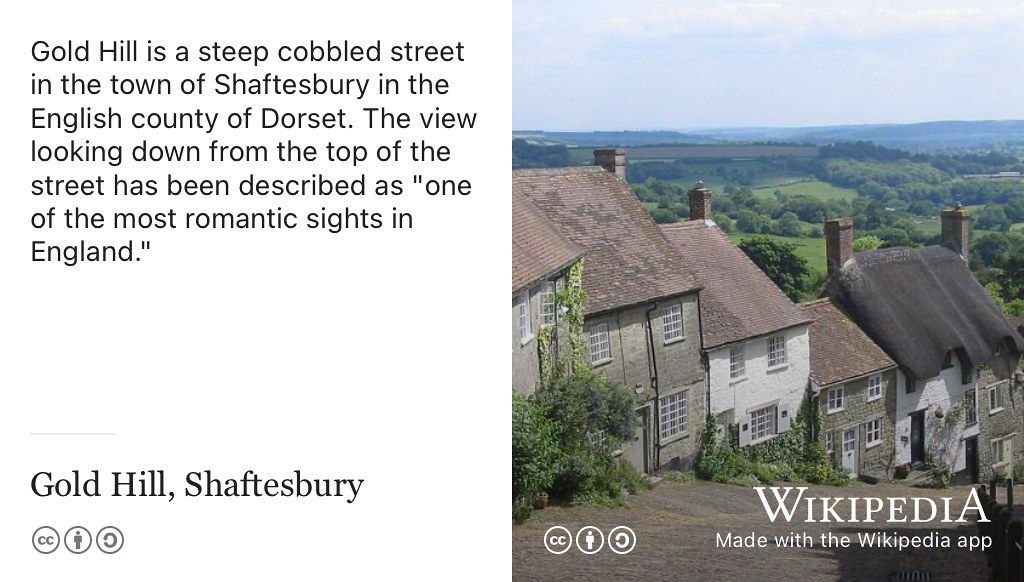
\includegraphics[width=1\linewidth]{images/shaftesbury} 

}

\caption{\href{https://en.wikipedia.org/wiki/Shaftesbury}{Shaftesbury} in Dorset is the home of \href{https://en.wikipedia.org/wiki/Gold_Hill,_Shaftesbury}{Gold Hill} and \href{https://en.wikipedia.org/wiki/Shaftesbury_School}{Shaftesbury School}. Image of Gold Hill by Sean Davis via Wikimedia Commons \href{https://w.wiki/3LhD}{w.wiki/3LhD} adapted using the \href{https://apps.apple.com/us/app/wikipedia/id324715238}{Wikipedia app}.}\label{fig:shaft-fig}
\end{figure}



So thanks Shaftesbury for lessons on top of Gold Hill and the Hovis Advert, one of Britain's best-loved adverts. \citep{hovisadvert} 🍞

\hypertarget{swindon}{%
\subsection{Thank you Swindon}\label{swindon}}

Thanks to headteacher \href{https://www.swindonadvertiser.co.uk/news/14113118.lydiard-school-looking-to-help-others-improve-gcse-results/}{Clive Zimmerman}, his team of staff, Mr M. Carter , Mr K. Thomas and the students of \href{https://en.wikipedia.org/wiki/Lydiard_Park_Academy}{Greendown Community School (now Lydiard Park Academy)} in Swindon, Wiltshire for hosting my second PGCE teaching placement. It was fun teaching you about waves using \href{https://twitter.com/alomshaha}{@Alom Shaha's} jelly babies and kebab sticks shown in figure \ref{fig:shaha-fig}.

\begin{figure}

{\centering 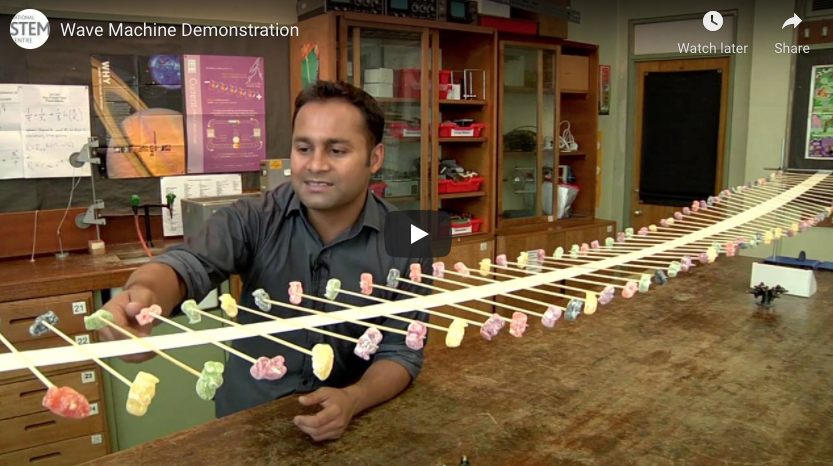
\includegraphics[width=0.99\linewidth]{images/youtube-alom} 

}

\caption{\href{https://alomshaha.com/}{Alom Shaha} demonstrates his awesome wave machine. Physics and jelly babies, what's not to like? \citep{youtube-alom} The image in the figure is a screenshot, watch the four minute video at \href{https://youtu.be/VE520z_ugcU}{youtu.be/VE520z\_ugcU}}\label{fig:shaha-fig}
\end{figure}



So thanks Swindon for being \href{https://en.wikipedia.org/wiki/Great_Western_Railway}{great and western} and \href{https://en.wikipedia.org/wiki/Swindon_Town_F.C.}{Swindon Town Football Club}, the best football team in the whole of the \href{https://en.wikipedia.org/wiki/West_Country}{West Country}. 🙏

\hypertarget{stockport}{%
\subsection{Thank you Stockport}\label{stockport}}

Thanks to headteacher Joanne Meredith, her team of staff and the students at \href{https://en.wikipedia.org/wiki/St_Anne\%27s_RC_Voluntary_Academy}{St.~Annes R.C. High School}, Stockport for hosting my \href{https://en.wikipedia.org/wiki/Newly_qualified_teacher}{Newly Qualified Teacher} (NQT) year. Thanks to Keith Doran and other members of the \href{https://www.elizabethanstockport.co.uk/}{alternative staff room} for your emotional, moral and practical support throughout the year. According to the \emph{Manchester Evening News}, St.~Anne's is ``the forgotten school'' \citep{stannes1, stannes2}, see figure \ref{fig:st-annes-fig}, but I'll never forget you or the lessons you taught me.

\begin{figure}

{\centering 
\includegraphics[width=1\linewidth]{images/st-annes-rc-high-school} 

}

\caption{Good governance is crucial to good schools. Many forgotten schools like \href{https://en.wikipedia.org/wiki/St_Anne\%27s_RC_Voluntary_Academy}{St.~Anne's R.C. High School}, and the thousands of children in the UK they educate every year, need help from skilled people like you on their governing boards. Why not serve your local community as a ``\href{https://en.wikipedia.org/wiki/Critical_friend}{critical friend}'' on the governing board of a school? All ages are welcome, but especially younger governors, see \href{https://www.theguardian.com/teacher-network/2015/mar/11/young-people-school-governors}{where are all the young school governors?} \citep{youngovernors} Take a look at \href{https://governorsforschools.org.uk/}{governorsforschools.org.uk}. Fair use image via Wikimedia Commons \href{https://w.wiki/3Swt}{w.wiki/3Swt} adapted using the \href{https://apps.apple.com/us/app/wikipedia/id324715238}{Wikipedia app}}\label{fig:st-annes-fig}
\end{figure}



So thanks Stockport for being Stockport, the magnificent \href{https://en.wikipedia.org/wiki/Stockport_Viaduct}{Stockport Viaduct} and for \href{https://en.wikipedia.org/wiki/Stockport_County_F.C.}{The Hatters}! It's all that matters, Stockport Hatters. 🙏

\hypertarget{schools}{%
\subsection{Thank you schools}\label{schools}}

Thanks to all the schools who interviewed me for my \href{https://en.wikipedia.org/wiki/Newly_qualified_teacher}{Newly Qualified Teacher} (NQT) year. Doing interview lessons, meeting your students and your senior leadership teams was a gruelling but fascinating magical mystery tour of the UK education system, both public and private. Although unsuccessful, these interviews were very productive failures:

\begin{itemize}
\tightlist
\item
  \href{https://en.wikipedia.org/wiki/Writhlington_School}{Writhlington School}, Radstock, Somerset, see their amazing Orchid project \href{https://wsbeorchids.org/thirty-years-of-the-writhlington-schools-orchid-project-a-teachers-view-by-simon-pugh-jones/}{wsbeorchids.org} run by \href{https://www.bristol.ac.uk/graduation/honorary-degrees/honorary-graduates-2019/simon-pugh-jones/}{Simon Pugh-Jones}
\item
  The \href{https://en.wikipedia.org/wiki/Cooper_School,_Bicester}{Cooper School, Bicester}, Oxfordshire, see their \href{https://www.youtube.com/watch?v=XdywHl2ZA-I}{teacher in my pocket} project
\item
  \href{https://en.wikipedia.org/wiki/St_John\%27s_Marlborough}{St John's Marlborough}, Wiltshire - not to be confused its posher and more famous next door neighbour \href{https://en.wikipedia.org/wiki/Marlborough_College}{Marlborough College}
\item
  \href{https://en.wikipedia.org/wiki/Oasis_Academy_Brislington}{Oasis Academy, Brislington}, Bristol
\item
  \href{https://en.wikipedia.org/wiki/Redland_Green_School}{Redland Green School}, Redland, Bristol
\item
  \href{https://en.wikipedia.org/wiki/The_John_of_Gaunt_School}{The John of Gaunt School}, Trowbridge, Wiltshire
\item
  \href{https://en.wikipedia.org/wiki/Didcot_Girls\%27_School}{Didcot Girls' School}, Didcot, Oxfordshire
\item
  \href{https://en.wikipedia.org/wiki/Cheltenham_Ladies\%27_College}{Cheltenham Ladies' College}, Cheltenham, Gloucestershire\footnote{As a newly trained Jedi knight, freshly armed with a PGCE, I was anxious for my first teaching job and momentarily considered using my pedagogical powers on the ``dark side'' of the force: private education. \citep{nicebutdim} Forgive me for I have sinned!}
\item
  \href{https://en.wikipedia.org/wiki/Blackburn_College,_Lancashire}{Blackburn College}, Lancashire ``I read the news today, oh boy! Four thousand holes in Blackburn, Lancashire'' \citep{adayinthelife}
\end{itemize}

So thanks schools, for schooling. 🙏

\hypertarget{oxford}{%
\subsection{Thank you Oxford}\label{oxford}}

Thanks to Martin Clutterbuck, Rebecca Clare, Richard O'Beirne, Simon Witter and everyone else at \href{https://www.flickr.com/photos/dullhunk/4042838703}{Blackwell Science Ltd} for looking after me in my first job as a freshly minted graduate.

Thanks to John Chelsom, Kal Ahmed, Clare Ashton, Tim Cave, Mavis Cournane, Eddie Dillon, Niki Dinsey, Phil Gooch, Antony Grinyer, Debbie Hagger, Gareth Hudson, Steve Horwood, Chris Joyce, Joe McCann, Keith McCann, Dave Nurse, Ian Packard, Mark Pengelly, Lillian Spearing, Omar Tamer and the rest of the team at CSW Informatics Ltd (\href{https://csw.co.uk/}{csw.co.uk}) for looking after me in my second job after Uni and teaching me about \href{https://oxin-centres.co.uk/}{Oxford Innovation}.

\begin{figure}

{\centering 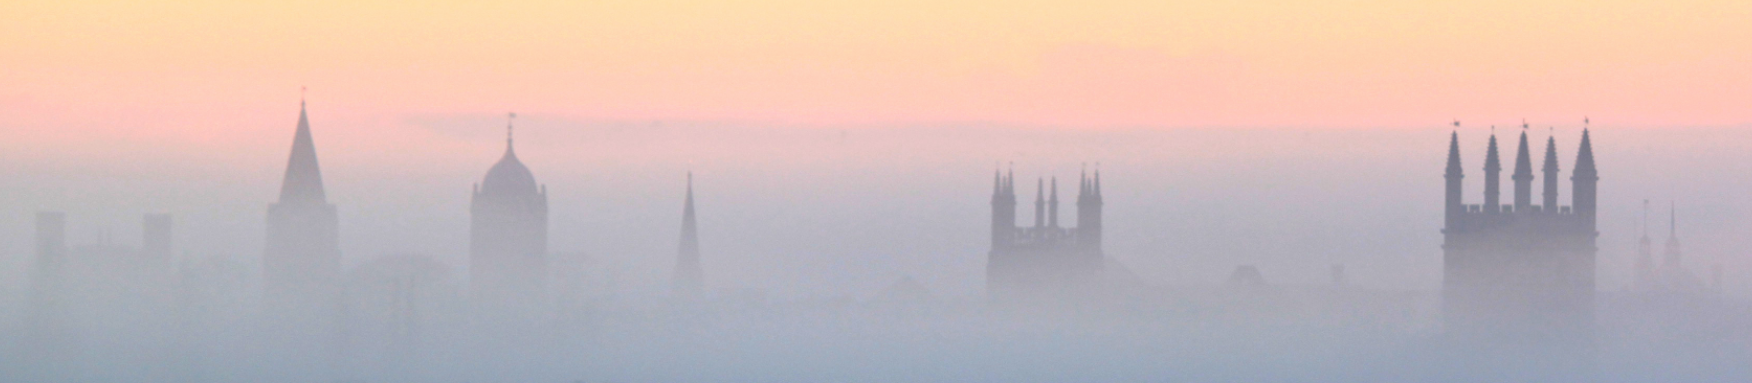
\includegraphics[width=1\linewidth]{images/dreaming-spires-oxford-sunrise} 

}

\caption{Looking West over Oxford's \href{https://en.wikipedia.org/wiki/Thyrsis_(poem)}{dreaming spires} from \href{https://en.wikipedia.org/wiki/South_Park,_Oxford}{South Park} towards the city of Oxford. Picture adapted from an original by Tejvan Pettinger on Wikimedia Commons \href{https://w.wiki/4Y25}{w.wiki/4Y25}}\label{fig:oxford-fig}
\end{figure}

Thanks to my fellow \href{https://xmlsummerschool.com/}{XML summer school} faculty: \href{https://www.bobdc.com/blog/}{Bob du Charme}, \href{https://twitter.com/psd}{Paul Downey}, \href{https://en.wikipedia.org/wiki/Michael_Howard_Kay}{Michael Kay}, \href{https://en.wikipedia.org/wiki/Jeni_Tennison}{Jeni Tennison} and \href{https://norman.walsh.name/}{Norman Walsh} for all the \texttt{\textless{}markup/\textgreater{}}.



Thanks to \href{https://en.wikipedia.org/wiki/Steven_A._Hill}{Steven A. Hill}, \href{https://en.wikipedia.org/wiki/Jane_A._Langdale}{Jane Langdale} and \href{https://en.wikipedia.org/wiki/Chris_J._Leaver}{Chris Leaver} at the University of Oxford (\href{https://www.plants.ox.ac.uk/}{plants.ox.ac.uk}) for interviewing me for a \href{https://www.gatsby.org.uk/}{Gatsby Charitable Foundation} scholarship for a DPhil. Thanks Chris for teaching me a painful but important lesson about the value of my education and grades.

So thanks Oxford for the dreaming spires, see figure \ref{fig:oxford-fig}. 🙏

\hypertarget{cambridge}{%
\subsection{Thank you Cambridge}\label{cambridge}}

Thanks to \href{https://en.wikipedia.org/wiki/Christoph_Steinbeck}{Christoph Steinbeck}, Nico Adams, Marcus Ennis, Janna Hastings, Paula de Matos, Adriano Dekker, Kenneth Haug, \href{https://twitter.com/jomcentyre}{Jo McEntyre}, Pablo Moreno, \href{https://twitter.com/drp_stuff}{Helen Parkinson} and Mark Rijnbeek at the \href{https://en.wikipedia.org/wiki/European_Bioinformatics_Institute}{European Bioinformatics Institute} (EBI, see figure \ref{fig:cambridge-fig}) for looking after me during my year in Cambridge.

\begin{figure}

{\centering 
\includegraphics[width=1\linewidth]{images/european-bioinformatics-institute} 

}

\caption{The European Bioinformatics Institute (EBI) is an outstation of the \href{https://en.wikipedia.org/wiki/European_Molecular_Biology_Laboratory}{European Molecular Biology Laboratory} (EMBL) in Hinxton, Cambridge, UK. Picture adapted from an original by \href{https://en.wikipedia.org/wiki/Magnus_Manske}{Magnus Manske} on Wikimedia Commons \href{https://w.wiki/4YQB}{w.wiki/4YQB} using the \href{https://apps.apple.com/us/app/wikipedia/id324715238}{Wikipedia app}}\label{fig:cambridge-fig}
\end{figure}



So thanks Cambridge for a really fen-tastic time in \href{https://en.wikipedia.org/wiki/Silicon_Fen}{Silicon Fen}. 🙏

\hypertarget{coventry}{%
\subsection{Thank you Coventry}\label{coventry}}

Thanks to \href{https://www.coventry.ac.uk/research/research-people/professor-phil-harris/}{Phil Harris}, Steph Harris, Alan Gear, Jackie Gear, Ally, Neil, Esther, Graham, \href{https://www.jeremycherfas.net/}{Jeremy Cherfas}, \href{https://cheshirenonprofitlaw.com/people/team/morgen/}{Morgen Cheshire}, \href{https://pureportal.coventry.ac.uk/en/persons/margi-lennartsson-turner}{Margi Lennartsson Turner}, Lady Godiva (see figure \ref{fig:coventry-fig}) and everyone else at the Henry Doubleday Research Association (HDRA) and Coventry University for hosting my industrial experience year during my undergraduate degree.

\begin{figure}

{\centering 
\includegraphics[width=1\linewidth]{images/godiva} 

}

\caption{Covered only in her long hair, \href{https://en.wikipedia.org/wiki/Lady_Godiva}{Lady Godiva} rode naked through the streets of Coventry to protest about taxation. Sadly I was 900 years too late to miss the spectacle but there is a statue of her in Broadgate you can ogle at. Painting of Godiva by \href{https://en.wikipedia.org/wiki/John_Collier_(painter)}{John Collier} adapted from an original on Wikimedia Commons \href{https://w.wiki/4aCU}{w.wiki/4aCU} using the \href{https://apps.apple.com/us/app/wikipedia/id324715238}{Wikipedia app}}\label{fig:coventry-fig}
\end{figure}



So thanks Coventry for naked women on horseback, a \href{https://en.wikipedia.org/wiki/Coventry_Cathedral}{magnificent cathedral} and the industrial experience. 🙏

\hypertarget{manchester}{%
\subsection{Thank you Manchester}\label{manchester}}

Thanks to Greater Mancunians Rob Aspin, Paul Bason, Martin Bryant, Gemma Cameron, Matthew Clark, Darren Dancey, Craig Dean, David Edmundson-Bird, Sherelle Fairweather, Shaun Fensom, Tony Foggett, Katie Gallagher, Emma Grant, David Haikney, Daniel Jamieson, Matt Jarvis, Ross Keeping, Val Kelly, Tony McGrath, Chris Marsh, Geraint North, Joe Sparrow, Martyn Spink, Julian Tait, Rachel Thompson, Wesley Verne, Paul Vlissidis, \href{https://en.wikipedia.org/wiki/Tony_Walsh_(poet)}{Tony Walsh} and Travis Walton for friendly Northern support and advice.

\begin{figure}

\includegraphics[width=0.33\linewidth]{images/Wednesday_Waggle} 
\includegraphics[width=0.33\linewidth]{images/Wednesday_Waggle} 
\includegraphics[width=0.33\linewidth]{images/Wednesday_Waggle} \caption{Bees symbolise both community and work ethic and have been a \href{https://en.wikipedia.org/wiki/Symbols_of_Manchester}{Manchester icon} since the industrial revolution in the 19th Century. We also use bees for our weekly \emph{Wednesday Waggle} jobs newsletter for students \href{https://waggle.cs.manchester.ac.uk/}{waggle.cs.manchester.ac.uk}. Buzzin'! \href{https://en.wikipedia.org/wiki/Waggle_dance}{Waggle dance} artwork by \href{https://visualthinkery.com/}{Visual Thinkery} is licensed under \href{https://creativecommons.org/licenses/by-nd/4.0/}{CC-BY-ND} 🐝}\label{fig:waggle-fig}
\end{figure}



So thanks Manchester for being Mancunian. \href{https://www.youtube.com/watch?v=PszMmYpQjPo}{This is the place}! 🙏

\hypertarget{moravians}{%
\subsection{Thank you Moravians}\label{moravians}}

Thanks to Thsespal Kundan, Principal of the \href{https://moravianinstitute.com/}{Moravian Institute in Rajpur}, Dehradun, \href{https://en.wikipedia.org/wiki/Uttar_Pradesh}{Uttar Pradesh}, India for hosting me and my friend Doug fresh out of high school on a gap year. We learned loads as visiting supply teachers of English and Mathematics, thanks to an introduction from a mutual contact Angus Barker. Thanks also to the \href{https://en.wikipedia.org/wiki/Fairfield_Moravian_Church}{Moravians in Manchester} at \href{https://en.wikipedia.org/wiki/Fairfield_High_School_for_Girls}{Fairfield High School for Girls} for hosting undergraduate Computer Science students as part of \href{http://www.cs.man.ac.uk/~hulld/coding-their-future.html}{coding their future}.

\begin{figure}

{\centering 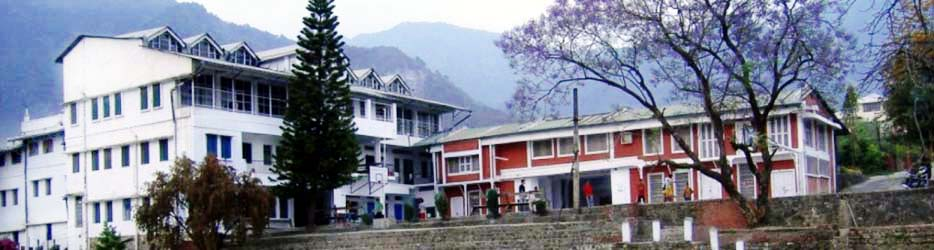
\includegraphics[width=1\linewidth]{images/moravian-insitute} 

}

\caption{The Moravian Institute lies in the foothills of the Himalayas between \href{https://en.wikipedia.org/wiki/Dehradun}{Dehradun} in the \href{https://en.wikipedia.org/wiki/Doon_Valley}{Doon Valley} and the hill station of \href{https://en.wikipedia.org/wiki/Mussoorie}{Mussoorie}. Situated between the \href{https://en.wikipedia.org/wiki/Yamuna}{Yamuna} and \href{https://en.wikipedia.org/wiki/Ganges}{Ganges}, the institute was founded in 1963 by the late Reverend Eliyah Thsetsan Phuntsog in \href{https://en.wikipedia.org/wiki/Ladakh}{Ladakh}, \href{https://en.wikipedia.org/wiki/Jammu_and_Kashmir_(state)}{Jammu \& Kashmir state} to provide education for \href{https://en.wikipedia.org/wiki/Tibetan_diaspora}{Tibetan refugees} fleeing from their homeland across the Himalayas.}\label{fig:moravian-fig}
\end{figure}



So thanks Moravians (and Angus) for life changing and formative experiences. 🙏

\hypertarget{influences}{%
\subsection{Thank you influencers}\label{influences}}

Some of the most important influences on this guidebook are people I've only met very briefly, virtually or not at all (yet).

\begin{itemize}
\tightlist
\item
  Thanks to \href{https://en.wikipedia.org/wiki/Gayle_Laakmann_McDowell}{Gayle Laakman McDowell} (\href{https://twitter.com/gayle}{@gayle}), for her cracking series of books \citep{techcareer, cracking, crackingpm, crackingthepmcareer} which have been very useful resources both for students I've worked with and me personally
\item
  Thanks to \href{https://en.wikipedia.org/wiki/Yihui_Xie}{Yihui Xie} (\href{https://github.com/yihui}{@yihui}) and contributors to \href{https://bookdown.org}{bookdown.org}, the software used to produce this book alongwith the comprehensive and well-written documentation on using it. \citep{xie2017, xie2015, xie2020}
\item
  Thanks to \href{https://en.wikipedia.org/wiki/Bronnie_Ware}{Bronnie Ware} for her \emph{\href{https://en.wikipedia.org/wiki/The_Top_Five_Regrets_of_the_Dying}{The Top Five Regrets of the Dying}} \citep{regrets} which helped me to re-align my priorities when they were all out of kilter
\item
  Thanks to blogging blokes on the interwebs whose words I've enjoyed reading. Your writing provides an existence proof that engineers and scientists should also be good communicators:

  \begin{itemize}
  \tightlist
  \item
    \href{https://en.wikipedia.org/wiki/Tim_Bray}{Tim Bray} at \href{https://www.tbray.org/ongoing/}{ongoing}
  \item
    Paul Downey at \href{https://blog.whatfettle.com/}{whatfettle.com}
  \item
    \href{https://en.wikipedia.org/wiki/Paul_Graham_(programmer)}{Paul Graham} at \href{http://paulgraham.com/}{paulgraham.com}
  \item
    \href{https://en.wikipedia.org/wiki/Andrew_D._Maynard}{Andrew Maynard} at \href{https://andrewmaynard.net/writing/}{andrewmaynard.net/writing}
  \item
    \href{https://en.wikipedia.org/wiki/Peter_Norvig}{Peter Norvig} at \href{https://norvig.com/}{norvig.com}
  \item
    Neil Saunders at \href{https://nsaunders.wordpress.com/blog/}{What you're doing is rather desperate}
  \item
    Greg Wilson at \href{https://third-bit.com/}{third-bit.com}
  \end{itemize}
\item
  Thanks to Jo Hobbs at Lancaster University for advice on placements and employability in undergraduate teaching
\item
  Thanks to \href{https://twitter.com/SRS_Sophie}{Sophie Milliken} for \emph{From Learner to Earner: A recruitment insider's guide for students wanting to achieve graduate job success} \citep{milliken} which draws useful distinctions between graduate jobs and graduate schemes
\end{itemize}

So, thanks influencers for being influential. 🙏

\hypertarget{github}{%
\subsection{Thank you githubbers}\label{github}}

Thanks to everyone who has contributed via github, listed below in order of github usernames. I will credit \emph{any} github contributors here, small or large. Even the typos, it all counts. I don't care what operating system you are using either, see figure \ref{fig:sticky-comics-fig}. You can easily add yourself to this roll call (see section \ref{contributing}) by correcting my delibreate mitsakes. 😉

Aman (\href{https://github.com/amanrana1}{@amanrana1}), Keith Mitchell (\href{https://github.com/apiadventures}{@apiadventures}), Zee Somji (\href{https://github.com/ezeethg}{@ezeethg}), iliketohelp (\href{https://github.com/iliketohelp}{@iliketohelp}), Jan Machacek (\href{https://github.com/janm399}{@janm399}), teobalmos (\href{https://github.com/teobalmos}{@teobalmos}), Tsvetankov (\href{https://github.com/Tsvetankov}{@Tsvetankov}), Richard Gourley (\href{https://github.com/richardgourley}{@richardgourley}), Tristan Maat (\href{https://github.com/TLATER}{@TLATER}), Safder Iqbal (\href{https://github.com/safderiqbal}{@safderiqbal})

\begin{figure}

{\centering 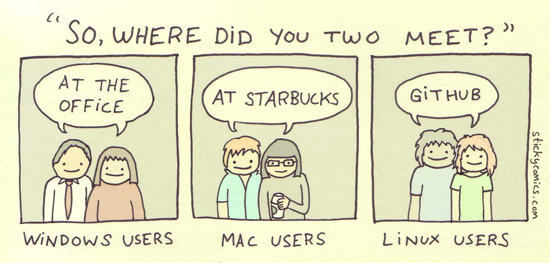
\includegraphics[width=1\linewidth]{images/os_couples} 

}

\caption{Windows users meet in the office, Mac users meet in Starbucks while Linux users meet on github. Comic by \href{https://www.linkedin.com/in/cmacauley}{Christiann MacAuley} at sticky comics \href{https://www.stickycomics.com/where-did-you-meet/}{stickycomics.com/where-did-you-meet} used with permission see \href{https://www.stickycomics.com/permissions/}{stickycomics.com/permissions}}\label{fig:sticky-comics-fig}
\end{figure}



So, thanks githubbers for cloning, forking, merging, pulling, adding, committing and pushing. 🙏

\hypertarget{wikipedians}{%
\subsection{Thank you Wikipedians}\label{wikipedians}}

Thanks to all the \href{https://en.wikipedia.org/wiki/Wikipedia:Wikipedians}{thousands of editors and engineers} that make Wikipedia one of the greatest communities on the internet, see figure \ref{fig:wikipedians-fig}.

\begin{figure}

{\centering 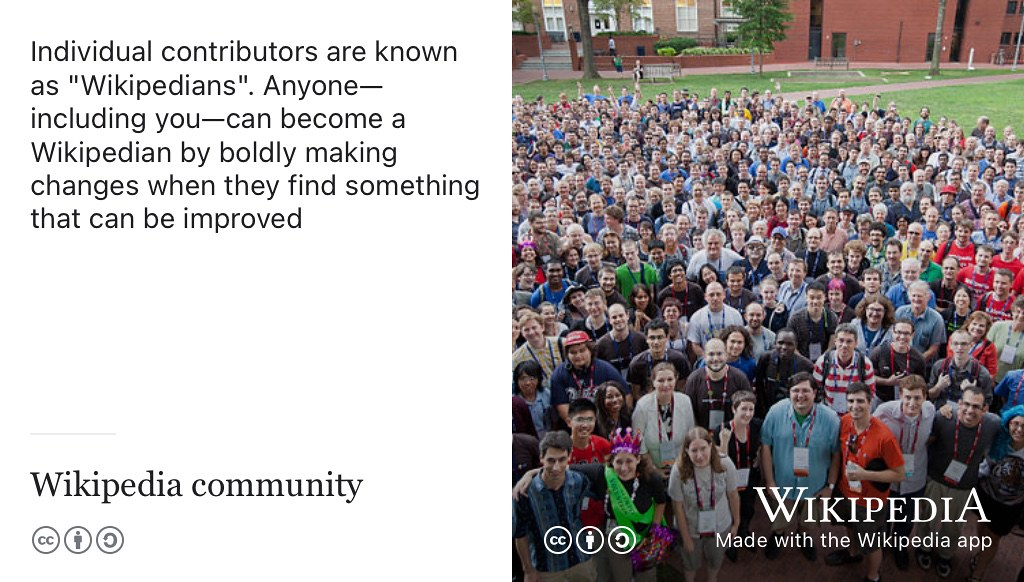
\includegraphics[width=0.99\linewidth]{images/wikipedians} 

}

\caption{A small fraction of the \href{https://en.wikipedia.org/wiki/Wikipedia_community}{Wikipedia community} that works to give free access to the sum of all human knowledge to every single person on the planet. CC BY-SA picture of Wikipedians gathered at the annual \href{https://en.wikipedia.org/wiki/Wikimania}{Wikimania conference} in 2012, adapted from an original by Helpameout on Wikimedia Commons \href{https://w.wiki/3YLJ}{w.wiki/3YLJ} using the \href{https://apps.apple.com/us/app/wikipedia/id324715238}{Wikipedia app}}\label{fig:wikipedians-fig}
\end{figure}



Special wiki-thanks to English speaking Wikipedians \href{https://en.wikipedia.org/wiki/Evan_Amos}{Evan Amos}, Abd Alsattar Ardati, \href{https://www.timeshighereducation.com/news/teaching-intelligence-putting-wikipedia-heart-class}{Caroline Ball}, Marianne Bamkin, Roger Bamford, \href{https://en.wikipedia.org/wiki/Alex_Bateman}{Alex Bateman}, Dan Brickley, John Byrne, Lucy Crompton-Reid, Daria Cybulska, Andrew Davidson, Paul Gardner, Madeleine Goodall, \href{https://en.wikipedia.org/wiki/Aaron_Halfaker}{Aaron Halfaker}, Melissa Highton, Eoin Houston, \href{https://royalsociety.org/topics-policy/projects/research-culture/changing-expectations/dr-darren-logan/}{Darren Logan}, \href{https://en.wikipedia.org/wiki/Magnus_Manske}{Magnus Manske}, \href{https://commons.wikimedia.org/wiki/User:Pigsonthewing}{Andy Mabbett}, Charles Matthews, Ewan McAndrew, Daniel Mietchen, Josh Minor, \href{https://en.wikipedia.org/wiki/Peter_Murray-Rust}{Peter Murray-Rust}, Richard Nevell, Frank Norman, \href{https://en.wikipedia.org/wiki/Roderic_D._M._Page}{Rod Page}, Bhavesh Patel, \href{https://www.mikepeel.net/}{Mike Peel}, \href{http://infobomb.org/}{Martin Poulter}, \href{https://en.wikipedia.org/wiki/Joseph_M._Reagle_Jr.}{Joseph Reagle}, \href{https://en.wikipedia.org/wiki/Gage_Skidmore}{Gage Skidmore}, \href{https://nitens.org/w/}{Dario Taraborelli}, Sara Thomas, \href{https://en.wikipedia.org/wiki/Denny_Vrande\%C4\%8Di\%C4\%87}{Denny Vrandečić}, Ian Watt, Alice White, \href{https://en.wikipedia.org/wiki/Jess_Wade}{Jessica Wade}, \href{https://en.wikipedia.org/wiki/Taha_Yasseri}{Taha Yasseri} for insights, \href{https://duncan.hull.name/2019/12/10/glasgow/}{inspiration}, \href{https://wiki-loves-scientists.org.uk/2020/05/21/wiki1000/}{support}, \href{https://apps.apple.com/us/app/wikipedia/id324715238}{software}, \href{https://www.wikidata.org/}{data}, \href{https://commons.wikimedia.org/}{pictures} and guidance. Thanks also for educating me on issues of equality, diversity and inclusion, especially gender and race.

So, thanks Wikipedians for being Wikipedia. 🙏

\hypertarget{visualthinkery}{%
\subsection{Thank you Bryan}\label{visualthinkery}}

Many of the illustrations for this book have been drawn by the very talented Bryan Mathers \href{https://twitter.com/BryanMMathers/}{@BryanMMathers} shown in figure \ref{fig:tedx-galway-fig}.

Bryan is an artist, visual thinker, entrepreneur and listener who turns stories into pictures. He also happens to have a Bachelors degree in Computer Science from the University of Glasgow. As a renaissance man, his combined skills in art, science and engineering made him the perfect fit for illustrating this guidebook. You can find out more about Bryan at \href{https://bryanmmathers.com}{bryanmathers.com} and \href{https://visualthinkery.com}{visualthinkery.com}. I'm \emph{sooo} glad we randomly bumped into each other at a conference.

\begin{figure}

{\centering 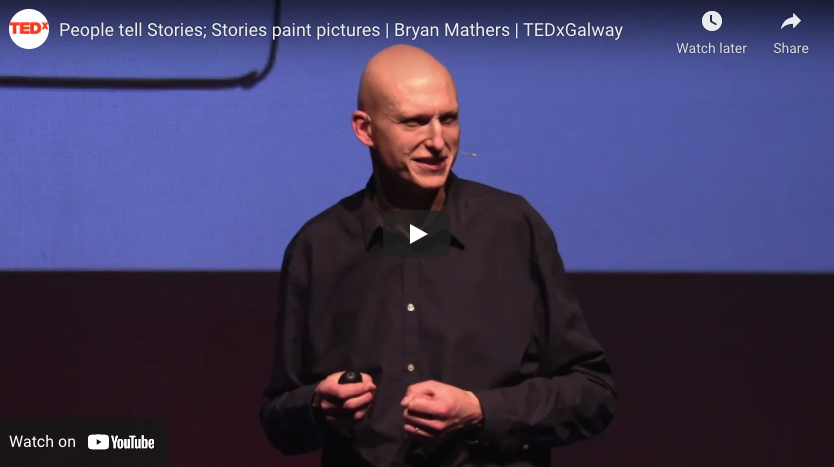
\includegraphics[width=1\linewidth]{images/bryan-mathers-tedx-galway} 

}

\caption{People tell stories and stories paint pictures. Bryan Mathers, who has illustrated much of this guidebook, telling stories at TEDxGalway in 2021. The image above is a screenshot, you can watch the full 15 minute talk at \href{https://youtu.be/IapGM5ZYBEw}{youtu.be/IapGM5ZYBEw}}\label{fig:tedx-galway-fig}
\end{figure}



So, thanks Bryan for your witty illustrations, this book wouldn't be the same without your visual thinkery. 🙏

\hypertarget{st-laurence}{%
\subsection{Thank you St Laurence}\label{st-laurence}}

Thanks to St Laurence school (\href{https://st-laurence.com/}{st-laurence.com}), a community I am proud and lucky to have grown up in. I'm especially grateful for the friendship of former St Laurence school students I've enjoyed music, cycling, football, walking, travelling, drinking and camaraderie with over the years. I can't name check you all here but \emph{Vive le Tour}, see figure \ref{fig:bradlads-fig}. I'm looking forward to our next adventure, gig, match, session or meetup.

\begin{figure}

{\centering 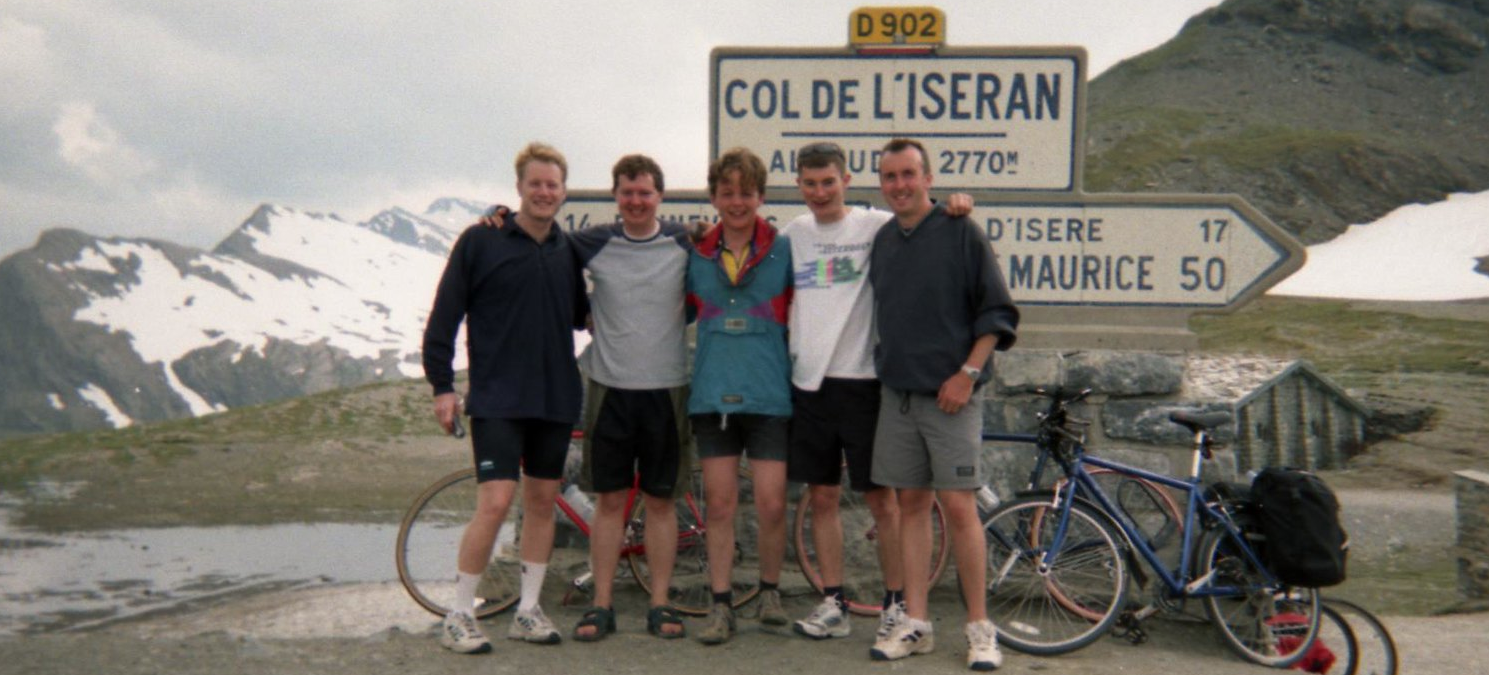
\includegraphics[width=1\linewidth]{images/kings-of-the-mountains-col-deliseran} 

}

\caption{Crossing the highest paved mountain pass in Europe, the \href{https://en.wikipedia.org/wiki/Col_de_l\%27Iseran}{Col de l'Iseran} in France, with my fellow alpinists and \href{https://en.wikipedia.org/wiki/King_of_the_Mountains}{Kings of the Mountains}: Jim, Dan, Doug and Dan. Rest in Peace Dan, you were a cherished friend, we all loved you and miss you terribly. Repose en paix. 🇫🇷}\label{fig:bradlads-fig}
\end{figure}



Special thanks my friend, former St Laurence school student and \href{https://st-laurence.com/sixth-form}{current sixth form head} Aidan Blowers for leading by example, wearing a white shirt in figure \ref{fig:uptown-funk-fig}. Aidan's performance as Lord of the Dance, which is highly recommended viewing, inspired the ongoing musical experiment that is \href{http://www.cs.man.ac.uk/~hulld/research.html\#tuningcomplete}{Tuning Complete}.

\begin{figure}

{\centering 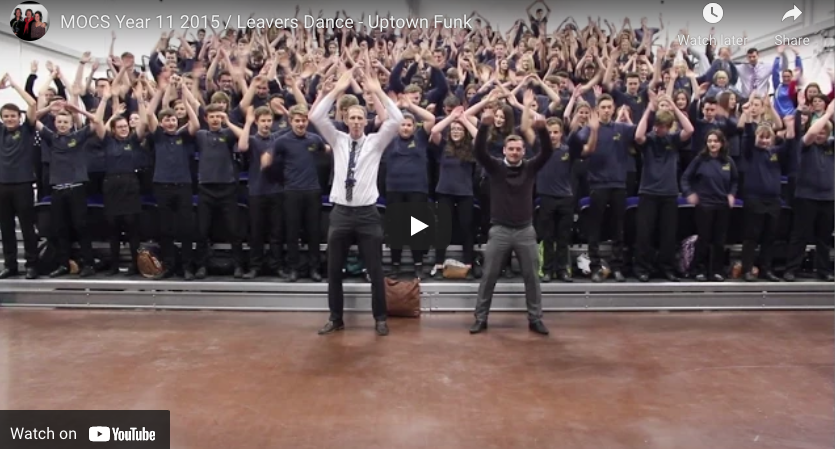
\includegraphics[width=1\linewidth]{images/youtube-mocs-uptown-funk} 

}

\caption{Year 11 leavers of \href{https://en.wikipedia.org/wiki/Melksham_Oak_Community_School}{Melksham Oak Community School} (MOCS) in Wiltshire dance to \href{https://en.wikipedia.org/wiki/Uptown_Funk}{Uptown Funk} with help from Mark Ronson, Bruno Mars and Aidan Blowers. The image above is a screenshot. Don't believe me, just watch, come on! \href{https://youtu.be/z8qH05teRMM}{youtu.be/z8qH05teRMM}}\label{fig:uptown-funk-fig}
\end{figure}



Thanks to all my teachers at St Laurence school, some of whom can be seen in figure \ref{fig:fitzmaurice-fig}.

\begin{figure}

{\centering 
\includegraphics[width=1\linewidth]{images/fitzmaurice-grammar-school} 

}

\caption{The staff of \href{https://en.wikipedia.org/wiki/Fitzmaurice_Grammar_School}{Fitzmaurice Grammar School} shortly before it merged with Trinity \href{https://en.wikipedia.org/wiki/Secondary_modern_school}{secondary modern school} to form the comprehensive \href{https://en.wikipedia.org/wiki/St_Laurence_School}{St Laurence school} in 1980. Back row, left to right, Alistair Thomson, Tony Hull, Geoff Swift, Peter Knight, John Warburton, John Blowers, Stuart Ferguson, Tim Wilbur, Bob Hawkes, Harry Haddon, John Blake. Centre: Joan Davis, Lynne Powell, Doug Anderson, Colin Steele, Virginia Evans, Joan Van Ryssen, Margaret Osbourne, Mireille (French Assistante), Sally Burden, Margaret Gadd. Front: Ken Revill, Marilyn Maundrell, Noreen Brady, Sid Johnson, Gerald Reid (Headmaster), Meg Tottle-Smith, Enid Wicheard, Diane Satterthwaite, Liz Buchanan, Margaret Hore. Picture via Keith Berry. \citep{bradfordonavon}}\label{fig:fitzmaurice-fig}
\end{figure}



Thanks to the rest of my St Laurence school teachers not pictured in figure \ref{fig:fitzmaurice-fig}. In alphabetical order: Phil Arthur, Sally Arthur, Maggie Bignell, \href{https://www.wiltshiretimes.co.uk/news/11774162.the-life-of-mrs-jackie-bolton/}{Jackie Bolton}, Tony Brooks, Dave Brush, \href{https://www.youtube.com/watch?v=Hg9irmFwFr8}{Andrew Butterworth}, Cathy Cooper, Ed Corrin, Mrs Davies, Brian Ellis, Myra Ettridge, Sue Glanville, Ms.~Gledhill, Roger Greenwood, Barry Hales, Amanda Hodges, \href{https://www.bathminervachoir.co.uk/our-accompanist}{Steven Hollas}, Mr Jones, Madame Lindsay, \href{https://www.amazon.co.uk/Karen-Long/e/B00NMARBTS}{Karen Long}, Sheila Macdonald, Simon Mitchell, Lee Musselwhite, Tim Noble, Roger Norgrove, Dave Pegg, Angela Pendennis, Brian Reynolds, Steve Stretch, Mr Sadler, Mike Sullivan, Phil Smith, Rob Townhill, Beryl Tucker, Chris Watters, \href{https://www.sourcewatch.org/index.php/James_Wetz}{James Wetz} and Bill Wheeler.

\begin{figure}

\includegraphics[width=0.0909\linewidth]{images/st-laurence-school-logo} 
\includegraphics[width=0.0909\linewidth]{images/st-laurence-school-logo} 
\includegraphics[width=0.0909\linewidth]{images/st-laurence-school-logo} 
\includegraphics[width=0.0909\linewidth]{images/st-laurence-school-logo} 
\includegraphics[width=0.0909\linewidth]{images/st-laurence-school-logo} 
\includegraphics[width=0.0909\linewidth]{images/st-laurence-school-logo} 
\includegraphics[width=0.0909\linewidth]{images/st-laurence-school-logo} 
\includegraphics[width=0.0909\linewidth]{images/st-laurence-school-logo} 
\includegraphics[width=0.0909\linewidth]{images/st-laurence-school-logo} 
\includegraphics[width=0.0909\linewidth]{images/st-laurence-school-logo} 
\includegraphics[width=0.0909\linewidth]{images/st-laurence-school-logo} \caption{The badge of St.~Laurence School is an adaptation of the Fitzmaurice badge with two \href{https://en.wikipedia.org/wiki/Gudgeon_(fish)}{gudgeon fish} symbolising the union of the two schools it was created from: Trinity secondary modern school and Fitzmaurice Grammar School}\label{fig:laurence-fig}
\end{figure}



So, thank you to the community that is St.~Laurence School, for educating me (and many others) the \href{https://en.wikipedia.org/wiki/West_Country}{West Country} way. Proper job! 🙏

\hypertarget{fitzmaurice}{%
\subsection{Thank you Fitzmaurice}\label{fitzmaurice}}

Thanks to my \href{https://www.fitzmauriceschool.info/}{Fitzmaurice Primary School} school teachers: Mrs Cripps, Miss Clarry, Mr Clay, Mr Fleming, Mr Jackson, \href{https://www.wiltshiretimes.co.uk/announcements/deaths/deaths/18007859.Betty_Knowles/}{Betty Knowles}, \href{https://www.dignityfunerals.co.uk/funeral-notices/21-11-2020-valerie-payne/}{Valerie Payne}, Miss Sheldon, \href{https://www.wiltshiretimes.co.uk/announcements/deaths/deaths/9828233.Hugh_Solomon/}{Hugh Solomon}, Miss Uncles and Mrs White. I used to foolishly think it was secondary schools that did all the serious teaching, but they'd be \emph{nowhere} without the crucial foundations laid in primary school. It takes a whole community (a village) to raise a child starting with primary school, see figure \ref{fig:clinton-fig}.

\begin{figure}

{\centering 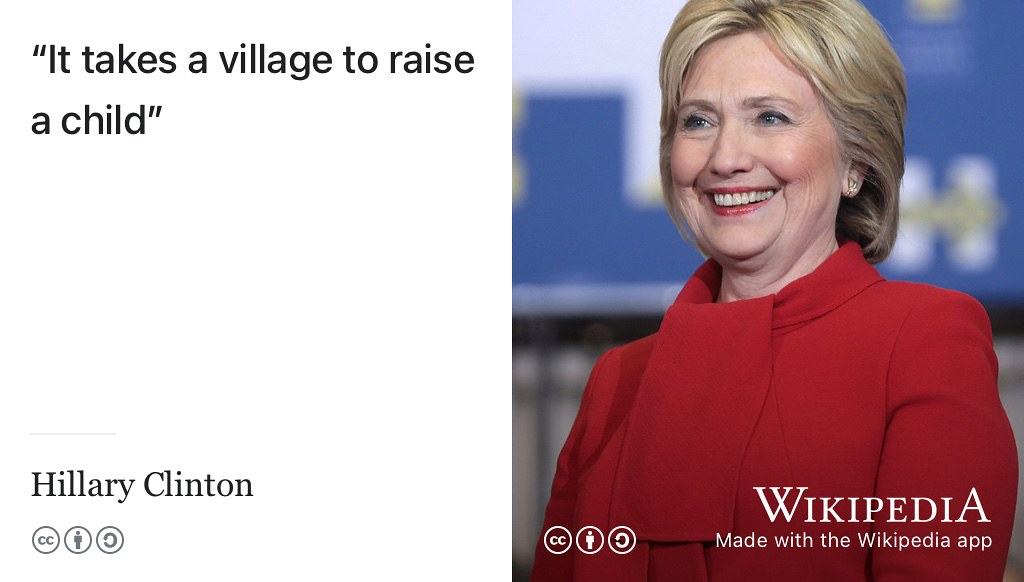
\includegraphics[width=1\linewidth]{images/hillary-clinton} 

}

\caption{\href{https://en.wikipedia.org/wiki/It_takes_a_village}{It takes a village} to raise a child. \citep{clinton} \href{https://en.wikipedia.org/wiki/Bradford-on-Avon}{Bradford-on-Avon} in Wiltshire is my village. Portrait of \href{https://en.wikipedia.org/wiki/Hillary_Clinton}{Hillary Clinton} speaking in 2016 by \href{https://en.wikipedia.org/wiki/Gage_Skidmore}{Gage Skidmore} on Wikimedia Commons \href{https://w.wiki/4Xrc}{w.wiki/4Xrc} adapted using the \href{https://apps.apple.com/us/app/wikipedia/id324715238}{Wikipedia app}}\label{fig:clinton-fig}
\end{figure}



So thanks Fitzmaurice Primary School and \href{https://en.wikipedia.org/wiki/Edmond_Fitzmaurice,_1st_Baron_Fitzmaurice}{Edmond Fitzmaurice} for laying solid foundations. 🙏

\hypertarget{family}{%
\subsection{Thank you family}\label{family}}

To my family: mum, dad, wife, son, brother, sister, μαμά, μπαμπά and extended family: I'm lucky to have been taught by you and that you've always been there when I needed you. 🇬🇷🇪🇺🇬🇧

So, thanks to all my family for your unconditional love. Σε αγαπώ παρα πολύ. 🙏

\hypertarget{duncan}{%
\section{About me}\label{duncan}}

Hello, my name is \href{http://www.cs.man.ac.uk/~hulld/}{Duncan Hull} and I wrote this guidebook for undergraduate and postgraduate students as part of my job at the University of Manchester where I'm a lecturer (≈ \href{https://en.wikipedia.org/wiki/Assistant_professor}{Assistant Professor}) in the \href{https://www.cs.manchester.ac.uk/}{Department of Computer Science}.

So what's \emph{my} story? Like many people, my path has been what \href{https://twitter.com/HelenTupper}{Helen Tupper} and Sarah Ellis call a ``\href{https://www.amazingif.com/}{squiggly career}'' rather than classic linear one. \citep{squigglybook, squigglytalk} I've been gainfully employed as a paperboy, supermarket cashier, shelf stacker, sausage factory worker, pork pie filler, chef, dogsbody, field assistant, database administrator, deli counter server, consultant, matchday steward, envelope stuffer, high school teacher, postdoc, research scientist, software engineer, lecturer, external examiner, tutor and scholar.

I've done a range of voluntary work too, serving as a competition judge, fundraiser, \href{https://codeclub.org}{code club} \& \href{https://coderdojo.com}{coderdojo} leader, rabble rouser, \href{https://www.manchesterdigital.com/}{digital council} member, \href{https://governorsforschools.org.uk/}{school governor}, curator, librarian, beer drinker, \href{https://wiki-loves-scientists.org.uk/}{wikipedia trainer}, \href{https://sigcse.cs.manchester.ac.uk/}{journal clubber} and editor. But as \href{https://en.wikipedia.org/wiki/Ronnie_Lane}{Ronnie Lane} and \href{https://en.wikipedia.org/wiki/Ronnie_Wood}{Ronnie Wood} (figure \ref{fig:faces-fig}) once said:

\begin{figure}

{\centering 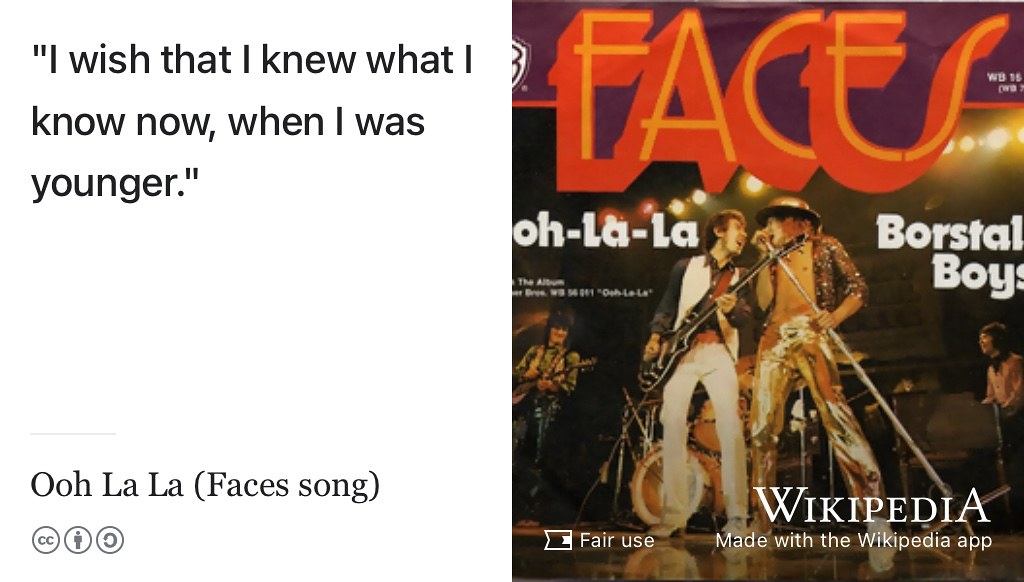
\includegraphics[width=0.99\linewidth]{images/faces} 

}

\caption{Hindsight is a great teacher. I wish that I knew what I know now, when I was younger, see \href{https://en.wikipedia.org/wiki/Ooh_La_La_(Faces_song)}{Ooh La La} \citep{faces} I've written some of what I know now in this guidebook, I hope you find it useful.}\label{fig:faces-fig}
\end{figure}



This guidebook documents some of what I know now, that I wish I'd known, when I was younger. If you're starting your career, I hope you find these insights and exercises useful. I've sat on both sides of the interview table, as interviewer and interviewee. I have had some spectacular failures, alongside some modest successes, and have included personal stories where they are relevant.

Most of what I have learned about employment comes from listening to, and watching students interact with employers as they take the first tentative steps in their careers. I've documented some of what they taught me, so reading this book may help you learn from some of their successes and failures.

\hypertarget{legal}{%
\section{Legal stuff}\label{legal}}

I am not a lawyer (\href{https://en.wikipedia.org/wiki/IANAL}{IANAL}) but any opinions expressed in this guidebook are my own and not representative of my current employer, the University of Manchester. This guidebook does not therefore, represent University policy.

\hypertarget{license}{%
\subsection{Licensing}\label{license}}

The \emph{text} of this guidebook is published under the \href{https://creativecommons.org/licenses/by-nc-nd/3.0/}{Creative Commons Attribution-NonCommercial-NoDerivs 3.0 License} (CC-BY-NC-ND) license see figure \ref{fig:cc-by-nc-nd-fig}.

\begin{figure}

{\centering 
\includegraphics[width=1\linewidth]{images/by-nc-nd} 

}

\caption{The \emph{text} of this guidebook is published under a \href{https://creativecommons.org/licenses/by-nc-nd/3.0/}{Creative Commons Attribution-NonCommercial-NoDerivs 3.0 License} (CC-BY-NC-ND) license which means you can copy and redistribute the material provided that you provide full attribution, do not use the material for commercial purposes and you do not make any derivative works.}\label{fig:cc-by-nc-nd-fig}
\end{figure}



This means you can copy and redistribute the written material provided that:

\begin{itemize}
\tightlist
\item
  You provide full attribution by linking directly to the original source
\item
  You do not use the material for commercial purposes
\item
  You do not make any derivative works
\end{itemize}

See the \href{https://creativecommons.org/licenses/by-nc-nd/3.0/}{full license} (CC-BY-NC-ND) for details.

The \emph{images} used in this guidebook are published under different licenses, depending on their source. For example, Bryan Mathers illustrations are licensed \href{https://creativecommons.org/licenses/by-nd/4.0/}{CC-BY-ND}, see figure \ref{fig:kapow-fig}. Other images have different licences, for example, images from Wikimedia Commons (\href{https://commons.wikimedia.org/}{commons.wikimedia.org}) are published under \href{https://creativecommons.org/licenses/by/2.0/}{CC-BY} or \href{https://creativecommons.org/licenses/by-sa/2.0/}{CC-BY-SA}, \href{https://en.wikipedia.org/wiki/Fair_use}{fair use} or \href{https://en.wikipedia.org/wiki/Public_domain}{public domain}. Each figure caption gives details for that images licence.

\begin{figure}

{\centering 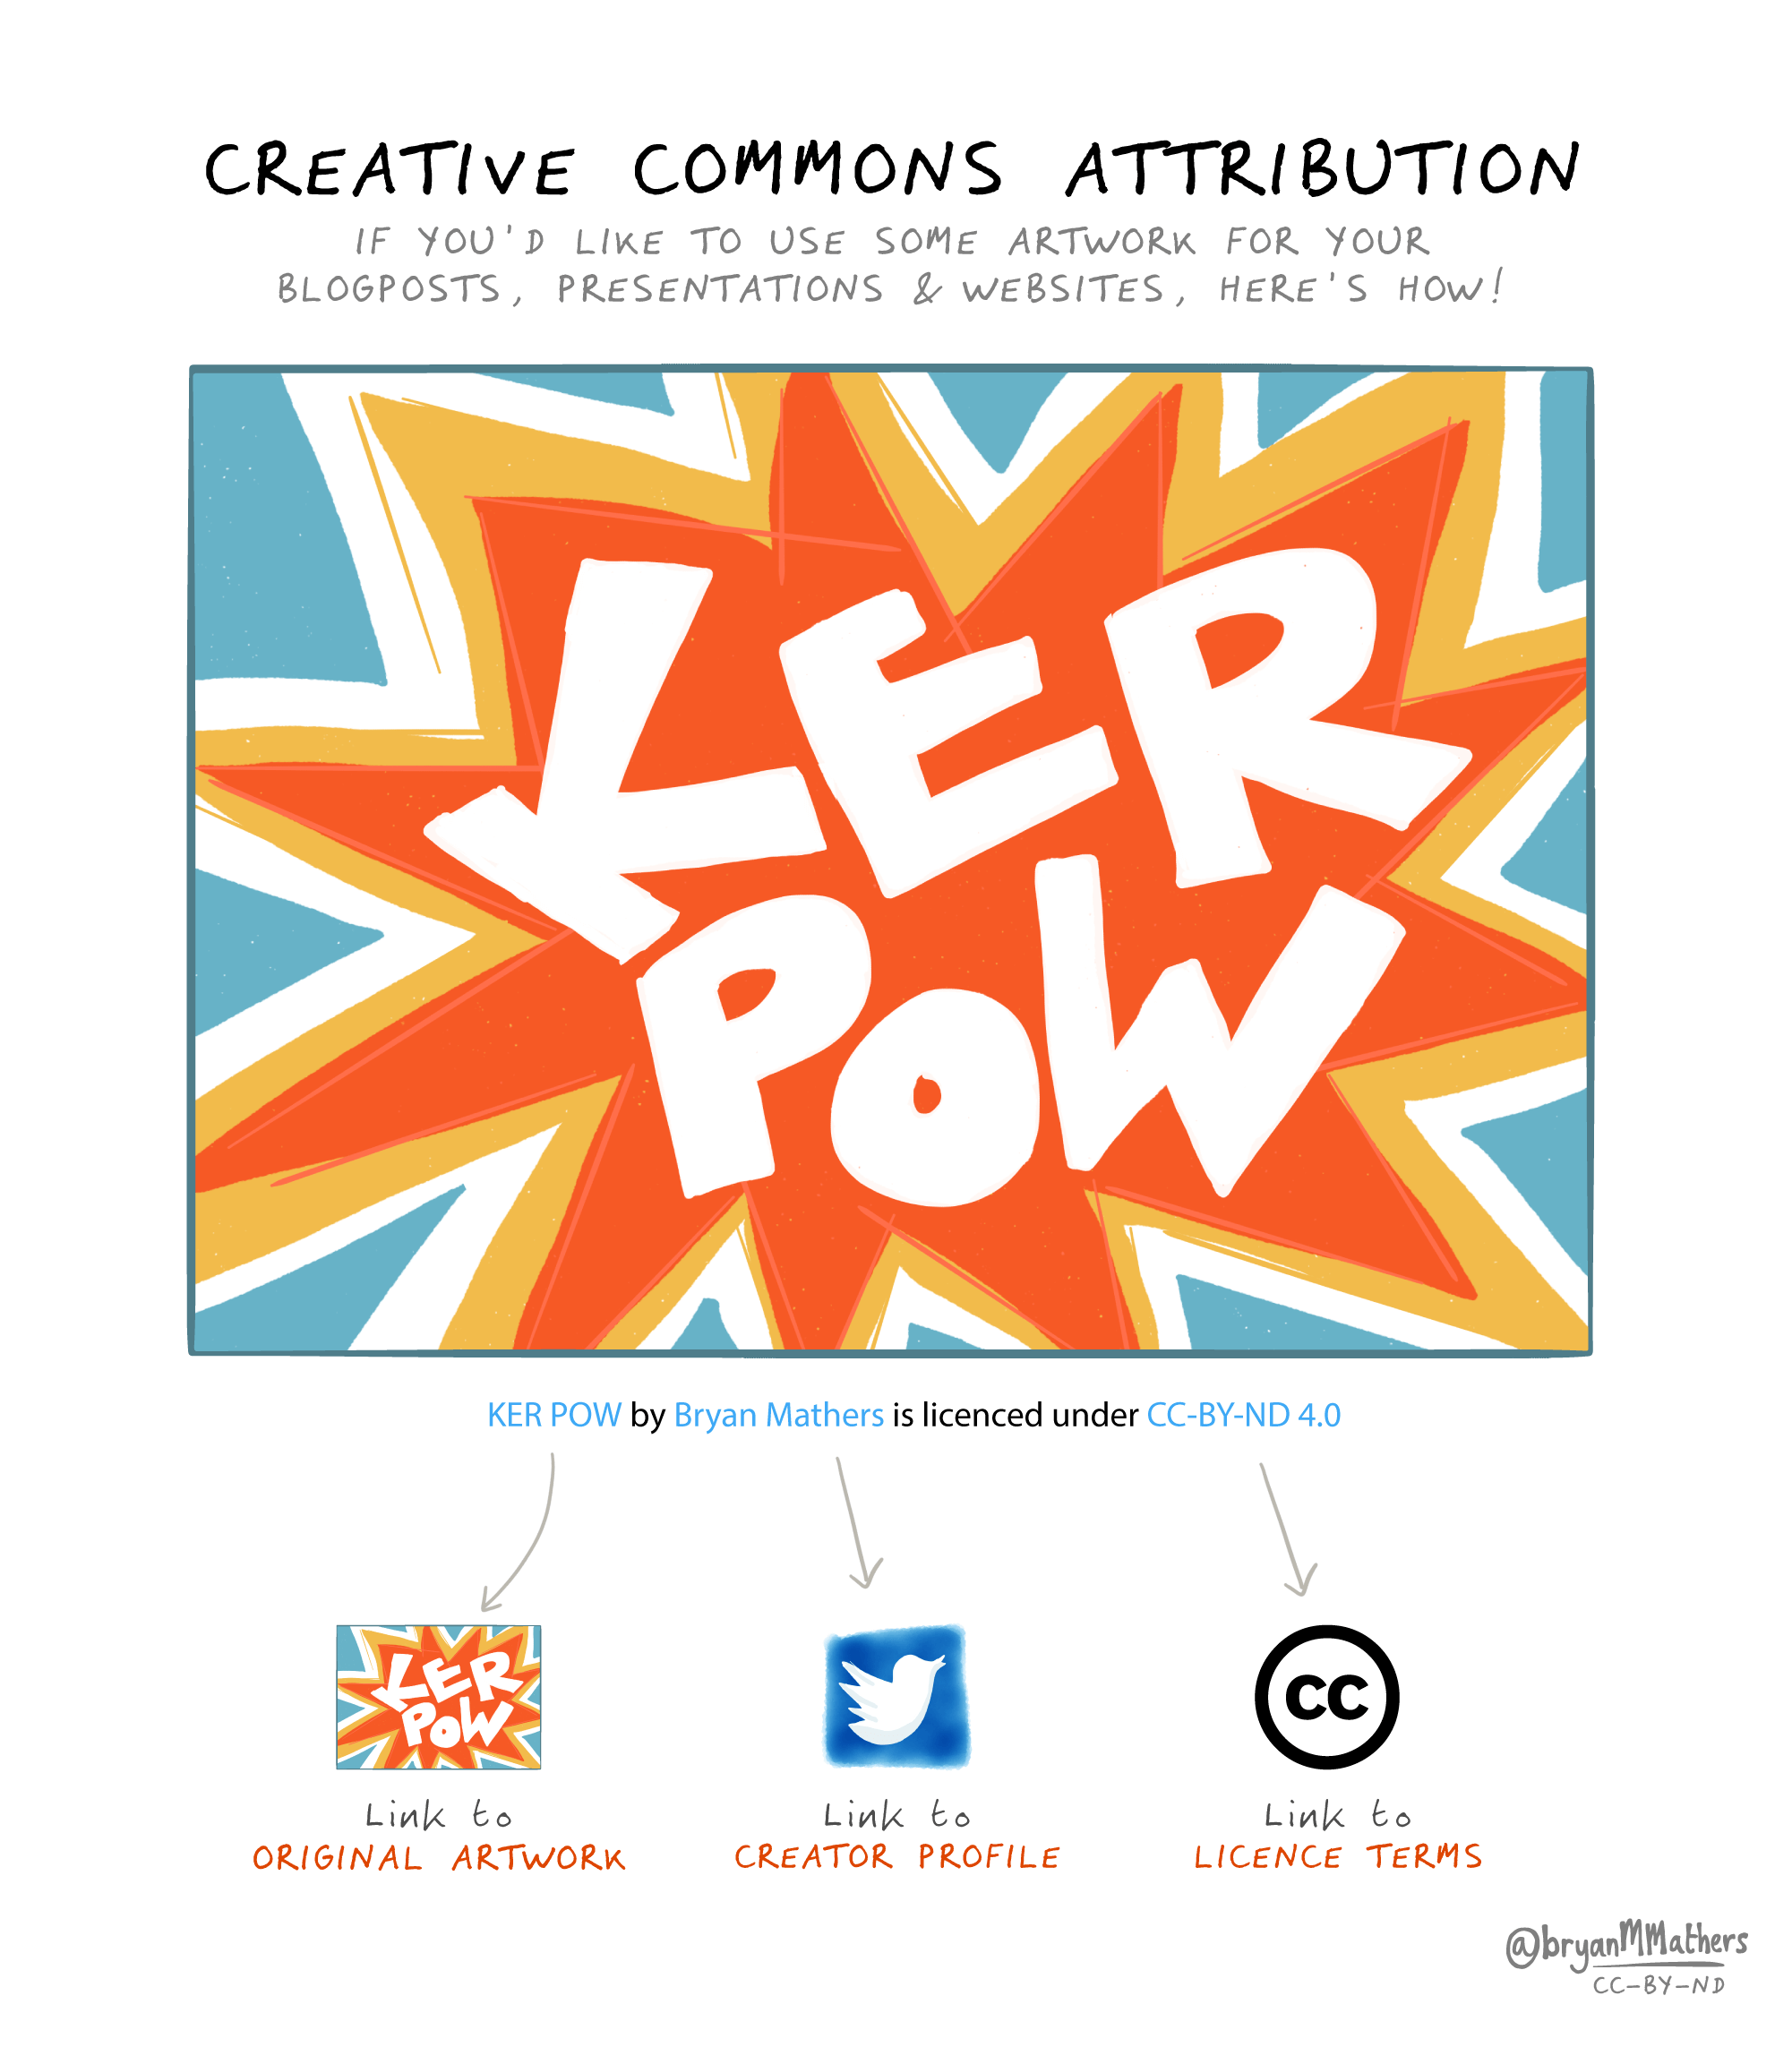
\includegraphics[width=1\linewidth]{images/CC-attribution-1} 

}

\caption{The \emph{images} in this guidebook are published under different licences, see each figures caption for details. Bryan Mathers illustrations are licensed CC-BY-ND, which means you should link to the original artwork, the creator profile and the licence terms. \href{https://bryanmmathers.com/cc-attribution/}{CC attribution} artwork by \href{https://visualthinkery.com/}{Visual Thinkery} is licenced under \href{https://creativecommons.org/licenses/by-nd/4.0/}{CC-BY-ND}}\label{fig:kapow-fig}
\end{figure}



\hypertarget{privacy}{%
\subsection{Your privacy}\label{privacy}}

This site is hosted on \href{https://www.netlify.com/}{netlify.com}, see the \href{https://www.netlify.com/privacy/}{netlify privacy policy}. This site also uses \href{https://docs.netlify.com/monitor-sites/analytics/}{netlify analytics} (server side) and \href{https://en.wikipedia.org/wiki/Google_Analytics}{Google Analytics} (client side) to understand our audience better. Both comply with the General Data Protection Regulation (GDPR). If you want to, you can opt out using the \href{https://tools.google.com/dlpage/gaoptout/}{Google Analytics Opt-out Browser Add-on}.

Some of these services use cookies. These can be disabled in your browser, see \href{https://www.allaboutcookies.org/manage-cookies/}{allaboutcookies.org/manage-cookies}

So now that we've dispensed with the formalities, let's look at why should you bother reading this guidebook in the first place.











\hypertarget{part-designing}{%
\part{DESIGNING}\label{part-designing}}

\hypertarget{rebooting}{%
\chapter{Rebooting your future}\label{rebooting}}

The first part of this book is about designing your future. So before we get started, we need to reboot and tackle a fundamental design issue. Why the hell would you want to bother reading this guidebook when you have so many other things to do right now? So:

\begin{itemize}
\tightlist
\item
  ✅ You are a busy person, YES!
\item
  ✅ Your time is a precious and finite resource, YES!
\item
  ✅ You could be spending that precious time right now in lots of other ways, YES!
\item
  ✅ There are mountains of self-help guides and courses already, YES!
\item
  ✅ Do you really need \emph{yet another} guidebook? YES!
\end{itemize}

You should read this guidebook because it is different to all the other guidebooks! It will help you design, test, build, debug and \texttt{code} your future in computing.

Before you start coding, we need to reboot. Come with me down the rabbit hole in figure \ref{fig:rabbit-fig} and let me explain\ldots{} 🐇

\begin{figure}

{\centering \includegraphics[width=0.7\linewidth]{images/Rabbit-hole} 

}

\caption{Shall we go down the rabbit hole? \href{https://bryanmmathers.com/rabbit-hole-learning/}{Rabbit Hole learning} by \href{https://visualthinkery.com}{Visual Thinkery} is licensed under \href{https://creativecommons.org/licenses/by-nd/4.0/}{CC-BY-ND}}\label{fig:rabbit-fig}
\end{figure}



\hypertarget{ilo1}{%
\section{What you will learn}\label{ilo1}}

After reading this chapter you will be able to:

\begin{itemize}
\tightlist
\item
  Reboot your future by

  \begin{itemize}
  \tightlist
  \item
    Setting your expectations for using this guidebook, and open some doors to your future
  \item
    Travelling down the rabbit hole into the underworld of employment
  \item
    Discussing some of the gaps that exist between formal education and employment and how you can bridge them
  \end{itemize}
\end{itemize}

\hypertarget{wonderland}{%
\section{Let's go down the rabbit hole}\label{wonderland}}

In the novel \emph{\href{https://en.wikipedia.org/wiki/Alice\%27s_Adventures_in_Wonderland}{Alice's Adventures in Wonderland}} \citep{wonderland}, the protagonist Alice follows a \href{https://en.wikipedia.org/wiki/White_Rabbit}{white rabbit} down a hole. What she discovers is a strange underground world populated by weird and wonderful characters. The world of work can sometimes be a mysterious underworld where you adventure in wonderland accompanied by colourful characters.

You will spend lots of time in this wonderland, potentially as much as 80,000 hours of your life. \citep{iip1, iip2} So join me down the rabbit hole, it's fun (honest), and sooner or later you'll have to come down here anyway. So open up the door to the new possibilities in your future.

\hypertarget{opening}{%
\section{Opening your future}\label{opening}}

Studying at University opens new doors to your future, some of which will take you down rabbit holes. As the poet \href{https://en.wikipedia.org/wiki/Lemn_Sissay}{Lemn Sissay} puts it (figure \ref{fig:lemn-fig}):

\begin{figure}

{\centering 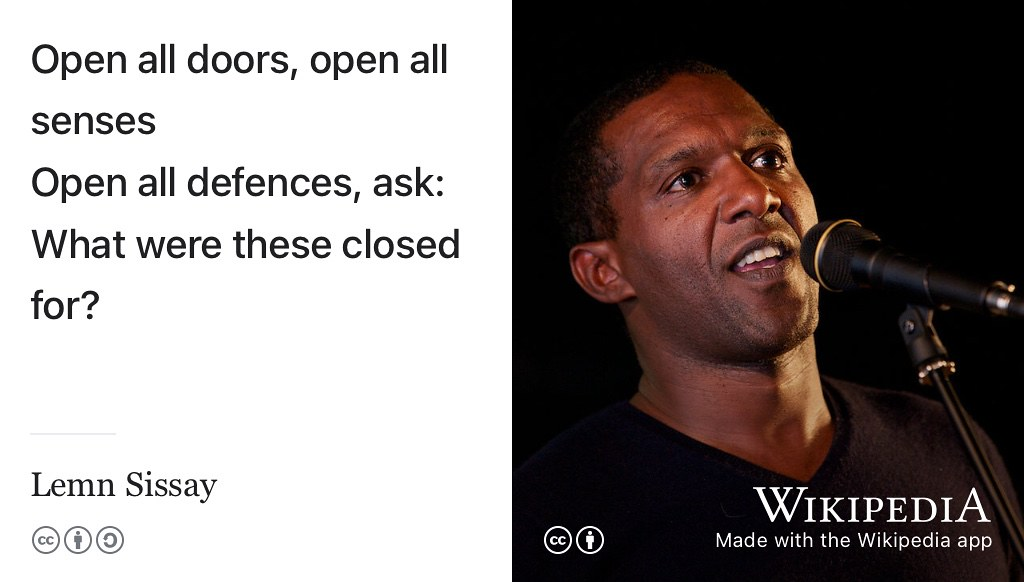
\includegraphics[width=0.99\linewidth]{images/lemninspire} 

}

\caption{Open all doors, open all senses, open all defences, ask: What were these closed for? From \emph{Inspire and be Inspired} by \href{https://en.wikipedia.org/wiki/Lemn_Sissay}{Lemn Sissay} whose poetry is even better when you hear it, rather than just read it \href{https://youtu.be/WzZs1w3NWzg}{youtu.be/WzZs1w3NWzg}. \citep{sissay} Portrait of Sissay speaking in 2010 by Philosophy Football via Wikimedia Commons \href{https://w.wiki/3VYT}{w.wiki/3VYT} adapted using the \href{https://apps.apple.com/gb/app/wikipedia/id324715238}{Wikipedia app}}\label{fig:lemn-fig}
\end{figure}



\hypertarget{roi}{%
\section{Maximising your future}\label{roi}}

As well as opening your future, studying at University is about \emph{investing} in your future. You're spending lots of your time and money at University. Hopefully, you've picked a subject that stimulates and challenges you intellectually while allowing you to find and develop your unique talents. But there's another reason that you probably chose to study at University and that was to improve your job prospects. This guidebook will:

\begin{enumerate}
\def\labelenumi{\arabic{enumi}.}
\tightlist
\item
  Help you maximise the return on the substantial investment of time and money (\href{https://en.wikipedia.org/wiki/Return_on_investment}{ROI}) you've put into your study
\item
  Give you an overview of important professional issues that are sometimes neglected or sidelined in University curricula
\item
  Highlight and review essential resources beyond this guidebook that will help with the above
\end{enumerate}

All of the resources that can help you are scattered around in lots of different places. There are books, there are videos, there are podcasts, there are websites and jobs boards. There are online courses, blogs, social media, newspaper columns, journal articles, marketing material and many other good resources. It is overwhelming.

\hypertarget{responsibility}{%
\section{Your future is your responsibility}\label{responsibility}}

When Andy Stanford-Clark started working at IBM, fresh out of University, his boss gave him the career advice shown in figure \ref{fig:andysc-fig}:

\begin{figure}

{\centering \includegraphics[width=0.99\linewidth]{images/nobody-cares-about-your-career-except-you} 

}

\caption{Nobody cares about your career except you. Quote via \href{https://en.wikipedia.org/wiki/Andy_Stanford-Clark}{Andy Stanford-Clark} \citep{andystanfordclark} to an unattributed IBM boss. Image of Andy by Gizmo\textasciitilde enwiki via Wikimedia Commons \href{https://w.wiki/3TSn}{w.wiki/3TSn} adapted using the \href{https://apps.apple.com/us/app/wikipedia/id324715238}{Wikipedia app}}\label{fig:andysc-fig}
\end{figure}



Andy is now Chief Technology Officer (CTO) and \href{https://en.wikipedia.org/wiki/IBM_Master_Inventor}{IBM Master inventor} in the UK so it was probably good advice. Another, slightly more positive way of putting the advice is, the person who cares \emph{most} about your career is you. So while there are people who can help design and build your future, ultimately it is \textbf{YOU} who has to take responsibility for the implementation (if you like, the \texttt{code}). The sooner you get coding the better.

At University, there are lots of people can help design and build your future: peers, friends, academic staff, your careers service, employers and your wider social and professional networks but ultimately it is \emph{your} responsibility to sort out whatever comes next. That might sound obvious but don't wait for somebody else to do it for you, because it probably won't happen.

\hypertarget{entitled}{%
\section{Your degree is not enough}\label{entitled}}

You have worked hard to get the grades you needed to get into University. You've spent (or are spending) a significant amount of time and money studying your chosen discipline. You are really \emph{geeking out} by going deep into your subject for a substantial period of time. Geekery, by which I mean \href{https://en.wikipedia.org/wiki/Geek}{being interested in a subject for its own sake}, is a \emph{good} thing. Earning the title \emph{geek} is a compliment, not an insult, and you should wear your geek badge with pride! Some people even say the geeks will inherit the earth, see figure \ref{fig:geekout-fig}. You are a geek, so where is \emph{your} inheritance?

\begin{figure}

{\centering \includegraphics[width=0.99\linewidth]{images/blessed-are-the-geeks} 

}

\caption{\href{https://en.wikipedia.org/wiki/Matthew_5:5}{Blessed are the \sout{meek} geeks, for they shall inherit the earth}. \citep{inherit, blessed} You are a geek, so where is your inheritance? Image of stained glass window by Norbert Schnitzler via Wikimedia Commons \href{https://w.wiki/43LN}{w.wiki/43LN} adapted using the \href{https://apps.apple.com/us/app/wikipedia/id324715238}{Wikipedia app}}\label{fig:geekout-fig}
\end{figure}



As a studious geek you might be tempted to believe that the world owes you something in return for all your geekiness. Unfortunately that's not the case.

At some point during or after your study, you might find yourself applying for a graduate job or graduate scheme. EVERYONE applying for these opportunities will have a degree or be rapidly on their way to getting one. So having a degree isn't going to set you apart much from your competition. Even having a first class degree may not distinguish you that much your competitors \citep{gradeinflation, firstclass}. Some employers would rather not know (or don't care) what University you went to, so your education might not make you stand out as much as you might like anyway. \citep{bigfour, eyfirm}

What \textbf{WILL} distinguish you from your competitors is:

\begin{itemize}
\tightlist
\item
  your experience, see chapter \ref{experiencing}
\item
  your projects, see section \ref{mycvpj}
\item
  your actions, see chapter \ref{actioning}
\item
  your communication skills, see chapters \ref{writing} and \ref{speaking}
\item
  any awards or honours you might have picked up along the way
\end{itemize}

If you think that your degree will be enough to get you the job you want, bear in mind that:

\begin{enumerate}
\def\labelenumi{\arabic{enumi}.}
\tightlist
\item
  There are more and more graduates, the UK for example recently passed the milestone of 50\% of young people going into higher education. This compares to just 15\% of over 18s who stayed in higher education in 1980 \citep{lotsofgrads}
\item
  The increase in the number of graduate schemes and graduate jobs has not kept pace with this growth in graduates which means that each graduate job or graduate scheme has more and more graduates applying for it
\item
  There are lots of graduates in your discipline. In the UK, for example, around 9,000 students graduate every year in Computer Science. If you're studying in the UK, what makes you different from the other 8,999 computer scientists graduating in your year?
\end{enumerate}

\begin{figure}

{\centering \includegraphics[width=1\linewidth]{cdyf_files/figure-latex/lotsofgrads-fig-1} 

}

\caption{Percentage of young people in the UK going into higher education between 1980 and 2018. Over the last forty years, the proportion of young people going into higher education has more than doubled from 15\% in 1980 to over 50\% in 2018. Data taken from BBC news article on \href{https://www.bbc.co.uk/news/education-49841620}{the symbolic target of 50\% at university reached} \citep{lotsofgrads}}\label{fig:lotsofgrads-fig}
\end{figure}



\begin{quote}
Computing is one of the largest subject areas in UK higher education, and is taught in almost every institution, graduating around 9,000 students every year --Sally Fincher \citep{fincherreview}
\end{quote}

Now, don't be disillusioned by the statistics because a degree can open doors to many careers in computing. What the data in Figure \ref{fig:lotsofgrads-fig} show is that you'll need to look beyond your formal education to distinguish yourself from your competition. Your degree can certainly help you start a career, and computer geekery is a commercially valuable skill but it is typically not enough by itself.

\hypertarget{thisstuffmatters}{%
\section{It's too late when you graduate}\label{thisstuffmatters}}

You might be tempted to postpone making difficult career decisions. I'll do it tomorrow. I'll do it next week. I'll do it next year. I'll finish this assignment. I'll finish this exam. I'll finish this semester. I'll finish my degree first, see figure \ref{fig:procrastination-fig}. Procrastination is a part of the \href{https://en.wikipedia.org/wiki/Human_condition}{human condition}. Software engineer \href{https://en.wikipedia.org/wiki/Paul_Graham_(programmer)}{Paul Graham} calls this \href{http://paulgraham.com/procrastination.html}{good and bad procrastination} \citep{procrastination}.

\begin{figure}

{\centering \includegraphics[width=0.99\linewidth]{images/procrastinator} 

}

\caption{\href{https://en.wikipedia.org/wiki/Procrastination}{Procrastination}: the attitude of ``I'll get my degree out of the way first then worry about jobs and careers when I finish University'' is bad procrastination. It's too late when you graduate to start thinking about what might come next \citep{procrastination} Stresssed procrastinator picture by MismibaTinasheMadando on Wikimedia Commons \href{https://w.wiki/3TXo}{w.wiki/3TXo}}\label{fig:procrastination-fig}
\end{figure}



Postponing decisions about your career is usually bad procrastination. It probably doesn't help that many of issues described and discussed in this book are typically not closely integrated into the curriculum in Higher Education. You'll often find them on the edges, or completely outside of, standard University curricula.

Despite being sidelined, these issues matter and it is in your own self interests to start thinking about them right now. According to recent estimates by \emph{Investors in People}, the average person spends \textbf{80,000 hours} working during their lifetime. \citep{iip2} So, \emph{whatever} you end up doing after University, you'll be spending a lot of time doing it. Difficult decisions often get sidelined but it is never too early to start thinking about them and doing something.

If you want to work for a big name like those in section \ref{bignames} or \ref{studentjobs}, many of the larger graduate employers expect you to have \emph{some} experience (see chapter \ref{experiencing}) \emph{before} you graduate. A large chunk of vacancies on graduate schemes are filled people who have already been employed as interns or placement students within that (or another) organisation. So the sooner you start investigating employers by getting some experience the better decisions you'll be able to make about what comes next. It's (usually) too late when you graduate.

That doesn't mean you have to know EXACTLY what you want to do when you finish. Lots of students don't and I certainly didn't when I graduated. I'd done a gap year teaching in India, two summer internships (in Sweden and the United States) and a year-in-industry in the UK and I \emph{still} graduated with \textbf{no clue} as to what I wanted to do next! The important thing is that you make a start, and sometimes knowing what you \textbf{don't} want to do is just as valuable as knowing what you want to do.

Computer scientists call this problem ``search space reduction'', \citep{searchspace} because you have a \href{https://en.wikipedia.org/wiki/Feasible_region}{feasible region} of future possibilities and you need to narrow down the candidates. You could think of coding your future as an \href{https://en.wikipedia.org/wiki/Optimization_problem}{optimisation problem}. Start optimising now because it's too late when you graduate. 🎓

\hypertarget{exams}{%
\section{Yes, this WILL be on the exam}\label{exams}}

Students love to ask their teachers ``\emph{will this be on the exam}''? The short answer is \textbf{YES} (and \textbf{NO})! Yes, this will be on the exam, but NO the exam won't be set by your University. Unlike other courses you've done, the examinations for this course aren't set by your University but by employers. Roughly speaking, there are three kinds of examinations that you'll need to get good at, shown in Table \ref{tab:examtable}

\begin{longtable}[]{@{}lll@{}}
\caption{\label{tab:examtable} Examining your future: The ``exams'' used by employers, what gets assessed and the grades you can get. For written ``exams'' see chapters \ref{writing} and \ref{debugging}, for speaking ``exams'' see chapter \ref{speaking} and for your employee ``exams'' see chapter \ref{surviving}.}\tabularnewline
\toprule
\begin{minipage}[b]{(\columnwidth - 2\tabcolsep) * \real{0.28}}\raggedright
Examination\strut
\end{minipage} & \begin{minipage}[b]{(\columnwidth - 2\tabcolsep) * \real{0.58}}\raggedright
What examiners are assessing\strut
\end{minipage} & \begin{minipage}[b]{(\columnwidth - 2\tabcolsep) * \real{0.14}}\raggedright
Grade\strut
\end{minipage}\tabularnewline
\midrule
\endfirsthead
\toprule
\begin{minipage}[b]{(\columnwidth - 2\tabcolsep) * \real{0.28}}\raggedright
Examination\strut
\end{minipage} & \begin{minipage}[b]{(\columnwidth - 2\tabcolsep) * \real{0.58}}\raggedright
What examiners are assessing\strut
\end{minipage} & \begin{minipage}[b]{(\columnwidth - 2\tabcolsep) * \real{0.14}}\raggedright
Grade\strut
\end{minipage}\tabularnewline
\midrule
\endhead
\begin{minipage}[t]{(\columnwidth - 2\tabcolsep) * \real{0.28}}\raggedright
CV, application form
covering letter\strut
\end{minipage} & \begin{minipage}[t]{(\columnwidth - 2\tabcolsep) * \real{0.58}}\raggedright
\begin{itemize}
\tightlist
\item
  Should we invite you to interview ?
\item
  Can you communicate well in writing?
\item
  What experience do you have?
\item
  What projects have you done?
\end{itemize}\strut
\end{minipage} & \begin{minipage}[t]{(\columnwidth - 2\tabcolsep) * \real{0.14}}\raggedright
pass/fail\strut
\end{minipage}\tabularnewline
\begin{minipage}[t]{(\columnwidth - 2\tabcolsep) * \real{0.28}}\raggedright
Interview\strut
\end{minipage} & \begin{minipage}[t]{(\columnwidth - 2\tabcolsep) * \real{0.58}}\raggedright
\begin{itemize}
\tightlist
\item
  Should we offer you a job?
\item
  Would we want you on our team?
\item
  Can you communicate well verbally?
\item
  Can you communicate well nonverbally?
\end{itemize}\strut
\end{minipage} & \begin{minipage}[t]{(\columnwidth - 2\tabcolsep) * \real{0.14}}\raggedright
pass/fail\strut
\end{minipage}\tabularnewline
\begin{minipage}[t]{(\columnwidth - 2\tabcolsep) * \real{0.28}}\raggedright
Employee performance\strut
\end{minipage} & \begin{minipage}[t]{(\columnwidth - 2\tabcolsep) * \real{0.58}}\raggedright
\begin{itemize}
\tightlist
\item
  Should we promote you?
\item
  Should we give you a pay rise?
\item
  Should we extend your contract?
\end{itemize}\strut
\end{minipage} & \begin{minipage}[t]{(\columnwidth - 2\tabcolsep) * \real{0.14}}\raggedright
pass/fail\strut
\end{minipage}\tabularnewline
\bottomrule
\end{longtable}

So, \emph{yes}, this will be on the exam, but \emph{no}, the exams are obviously not set, administered, invigilated and marked by academics at your University. The exams are set by employers and the results are \textbf{brutally binary}:

\begin{itemize}
\tightlist
\item
  \textbf{PASS}: you've got the interview, job or promotion or\ldots{}
\item
  \textbf{FAIL}: none of the above. Next!
\end{itemize}

One of the challenging things about employers exams are, they typically do not have the bandwidth to give applicants useful feedback, other than a simple pass or fail. When it comes to job applications software engineer \href{https://en.wikipedia.org/wiki/Gayle_Laakmann_McDowell}{Gayle Laakmann McDowell} calls this the ``black hole''. The gravitational force of employers black holes is so strong that no CV or Résumé can escape, we'll say more about this in chapter \ref{debugging} on debugging your future.

\begin{figure}

{\centering \includegraphics[width=1\linewidth]{images/Gimme Some Credit - Sketch} 

}

\caption{So \emph{no} this will not be on the exam set by University, but \emph{yes} it will be on the exams set by employers. Some of the most important exams you sit at (and after) University are set by employers. This guidebook will help you prepare for those exams and increase your chances of passing them. Gimme some credit figure by \href{https://visualthinkery.com/}{Visual Thinkery} is licensed under \href{https://creativecommons.org/licenses/by-nd/4.0/}{CC-BY-ND}}\label{fig:exam-fig}
\end{figure}



It's a similar story with interviews, if you fluffed and interview question or came across badly, it can be really difficult to find out from the employer what you did wrong.

\hypertarget{activities}{%
\section{Practicing your future}\label{activities}}

There are practical exercises, for you to get your hands dirty with. Each chapter incorporates activities including individual exercises, group exercises, quizzes and points for wider discussion. You'll get a lot more out of this guidebook by doing the activities, rather than just reading it.

\hypertarget{relatedwork}{%
\section{Navigating your future}\label{relatedwork}}

There are \textbf{lots} of resources out there that offer self-help, career advice and techniques for self-improvement. It can be hard to know where to start, or even how to find your way around the mountains of advice.

\begin{figure}

{\centering \includegraphics[width=1\linewidth]{images/shelfie} 

}

\caption{There are tonnes of resources out there offering advice on a huge range of professional issues. You can't read them all, but this guide aims to help you navigate the resources that will be most use to you}\label{fig:shelfie-fig}
\end{figure}



Lots of professional advice is readily available, but how will you navigate it? This book signposts you to what I think are the most important resources, each chapter has a signposts section, and they are all gathered together in the signpost at the end alongside everything (yes, EVERYTHING!) that this guidebook cites in the references, chapter \ref{reading}.

\hypertarget{crediting}{%
\section{Crediting your future}\label{crediting}}

Get credit for your contributions. As well as being openly accessible on the web, this book is open source too. What this means is, you can contribute in several ways described in section \ref{contributing}. All the written content for this guidebook is licensed under CC-BY-NC-ND, see the license in section \ref{license}.

\hypertarget{thinkdifferent}{%
\section{Your future is different}\label{thinkdifferent}}

I wrote this guidebook because I needed a resource for students to help them design, build, test, hack and debug their futures. I needed a book that could help students compete for jobs while at University, or shortly after graduating. I could not find anything suitable that met all the requirements of the students I was teaching. So I wrote this one which contains some new material and recommends the best resources if you want to know more. These are found in the signposts sections of each chapter.

This book aims to combine these perspectives and to be different from existing resources in the following ways:

\hypertarget{signposted}{%
\subsection{Your future is signposted}\label{signposted}}

Some career resources claim (or imply) that they are the \emph{all you will need} to solve a particular problem or worse: solve \emph{all of your problems}! Just buy this book, do this course, watch this video, listen to this podcast and all your problems will go away! Rather than continue this trend, this book \textbf{signposts} some of the most useful resources, see figure \ref{fig:signposting-fig}.

\begin{figure}

{\centering \includegraphics[width=1\linewidth]{images/signposting} 

}

\caption{Wondering which way to go at the \href{https://en.wikipedia.org/wiki/Traffic_sign}{traffic sign}? I've signposted the resources that will help you navigate the start of your professional journey. Which route will you take? Picture of a signpost in the \href{https://en.wikipedia.org/wiki/\%C3\%85land_Islands}{Åland Islands}, Finland by Sal via Wikimedia Commons \href{https://w.wiki/3Xop}{w.wiki/3Xop} adapted using the \href{https://apps.apple.com/us/app/wikipedia/id324715238}{Wikipedia app}}\label{fig:signposting-fig}
\end{figure}



Scientists call signposting \textbf{citation}, so I've signposted and cited sources in this guidebook so that you can :

\begin{enumerate}
\def\labelenumi{\arabic{enumi}.}
\tightlist
\item
  Follow them if the destinations are interesting or useful
\item
  Check and verify any facts and claims I make in this book for yourself
\end{enumerate}

While this guidebook cites lots of resources, some of them are more important than others. Each chapter summarises these in a signposts section. You'll find everything else in the references, chapter \ref{reading}. University and public libraries may also have physical and electronic copies of some of the books listed here.

We're not suggesting that you read \emph{all} these books right now, but that if a particular chapter has piqued your interest, these signposts are good places to keep going, if you haven't already read them. I hope you'll find these signposts handy for navigating the mountains of advice. Not all who wander are lost. 🗺️🧭

\hypertarget{study}{%
\subsection{Your future is guided}\label{study}}

This guidebook to your future accompanies a course that has been co-designed by students for students, with input from academics and employers. It unites several disparate themes into one coherent story, from fundamental questions about identity and wellbeing through to more applied and practical advice on job hunting, career progression and life after University. Resources that do this are typically scattered around in many different places. There is usually no narrative to tie them all together to help students navigate the mountains of advice as embark on the first stages of their careers.

Although this is a course guidebook used in the second year undergraduate teaching, you don't need to be enrolled on the course to benefit from reading it, watching the videos and doing the exercises and coding challenges.

\hypertarget{version}{%
\subsection{Your future is constantly updated}\label{version}}

You are reading the alpha version, the \href{https://en.wikipedia.org/wiki/Minimum_viable_product}{Minimum Viable Product} (MVP) of this guidebook, last updated on 21 December, 2021. That's software engineer talk for saying it isn't finished yet. Subsequent versions, will be continuously and iteratively released on a daily and weekly basis. They will include:

\begin{itemize}
\tightlist
\item
  More quizzes for better interactivity
\item
  More videos on the \href{https://www.youtube.com/channel/UCLBv_u8JmyUPqmRALIjVnLg}{Coding your Future YouTube channel}
\item
  Audio interviews with Students in the \emph{Coding your Future podcast} in chapter \ref{hearing}
\item
  More illustrations throughout the book
\item
  Improved content, finish incomplete chapters
\item
  Fix bugs and typos
\item
  Your suggestions for improvements and corrections, via github etc see section \ref{contributing}
\end{itemize}

I'm taking a \href{https://en.wikipedia.org/wiki/Release_early,_release_often}{release early, release often} \citep{Raymond1999} approach to publishing this guidebook, you could call it agile book development, see figure \ref{fig:agile-vs-waterfall-fig} \citep{realagile}

\begin{figure}

{\centering \includegraphics[width=1\linewidth]{images/agile-vs-waterfall} 

}

\caption{\href{https://en.wikipedia.org/wiki/Agile_software_development}{Agile software developers} make it up as they go along, whereas \href{https://en.wikipedia.org/wiki/Waterfall_model}{waterfalling software developers} make it all up at the beginning and then live with the consequences. It's the same with natural language engineering (books). I'm making it up as I go along, using agile book development methods. Women who code image by Justice Okai Allotey via Wikimedia Commons \href{https://w.wiki/3Xnk}{w.wiki/3Xnk} adapted using the \href{https://apps.apple.com/us/app/wikipedia/id324715238}{Wikipedia app}}\label{fig:agile-vs-waterfall-fig}
\end{figure}



\hypertarget{firstperson}{%
\subsection{Your future is personal}\label{firstperson}}

A lot of scientific and technical writing is written in the third person or passive voice, which is fine for academic writing, but can alienate readers. I have opted to use first person narrative where possible as it is shorter, and hopefully more engaging for you to read. \citep{googler} Where relevant, I've told personal stories to illustrate key points.

\hypertarget{openaccess}{%
\subsection{Your future has no paywall}\label{openaccess}}

You don't need to pay anything to read this book online because its not hiding behind a \href{https://en.wikipedia.org/wiki/Paywall}{paywall}, see section \ref{license}. Publishing this guidebook online makes it findable and accessible, something that isn't true of knowledge locked up inside other books.

Because this guidebook is online, it is searchable, browsable and linkable. You can link to whatever level you like, top level, chapter level and to every section and subsection level. Everything important has a Uniform Resource Locator (\href{https://en.wikipedia.org/wiki/URL}{URL}).

\hypertarget{nologin}{%
\subsection{Your future has no login}\label{nologin}}

You don't need to login to anything to use this guidebook either. Hurrah! One less password to remember.

\hypertarget{av}{%
\subsection{Your future has audio \& video}\label{av}}

This book is not just words and pictures, but includes audio and video as well, especially:

\begin{enumerate}
\def\labelenumi{\arabic{enumi}.}
\tightlist
\item
  videos produced by third parties that are worth watching
\item
  audio produced by third parties that are worth listening to, either individual episodes or whole series
\item
  short videos produced by me, which augment the written content of this book, see the \href{https://www.youtube.com/channel/UCLBv_u8JmyUPqmRALIjVnLg}{Coding your Future YouTube channel}
\item
  the coding your future podcast which interviews undergraduate students
\end{enumerate}

\hypertarget{engage}{%
\section{Engaging with your future}\label{engage}}

I've tried to make the content of this book as engaging as possible by including pictures and conversations. \emph{Your future} is deliberately playful and light-hearted. If you think this guidebook can be improved, let me know via the mechanisms described in section \ref{contributing}. I always welcome constructive feedback, especially when it comes via a pull request. Engage, see figure \ref{fig:startrek-fig}.

\begin{figure}

{\centering \includegraphics[width=1\linewidth]{images/captain-jean-luc-picard} 

}

\caption{This is Captain \href{https://en.wikipedia.org/wiki/Jean-Luc_Picard}{Jean-Luc Picard} of the Starship \emph{Enterprise}. Engage! Fair use image of actor \href{https://en.wikipedia.org/wiki/Patrick_Stewart}{Patrick Stewart} performing in \emph{Star Trek} adapted using the \href{https://apps.apple.com/us/app/wikipedia/id324715238}{Wikipedia app}. Make it so.}\label{fig:startrek-fig}
\end{figure}



\hypertarget{sign1}{%
\section{Signposting your future}\label{sign1}}

Each chapter in this book has a signposts section, highlighting key reading, watching or listening you could do next. This chapter has addressed the question of \textbf{why should you bother coding your future}? The answer is that your future is your responsibility and no-one elses. There are lots of people can help shape your future, but none more than yourself. Software engineer \href{https://en.wikipedia.org/wiki/Robert_C._Martin}{Robert C. Martin} argues this point in his book \emph{The Clean Coder: A Code of Conduct for Professional Programmers}. \citep{cleancoder}

What's good about \emph{The Clean Coder} is that it is short (only 200 pages), well written and to the point. The main part of the book covers professional issues in software engineering, some of which I discuss further in chapter \ref{surviving}, \emph{surviving your future}.

\hypertarget{tldr1}{%
\section{Summarising your future}\label{tldr1}}

If all that was \href{https://en.wiktionary.org/wiki/too_long;_didn\%27t_read}{too long, didn't read} (TL;DR) for you, then you'll be relieved to hear that each chapter has a TL;DR (executive) summary.

\begin{figure}

{\centering \includegraphics[width=1\linewidth]{images/tldr} 

}

\caption{There's always more stuff you should be \href{https://en.wikipedia.org/wiki/Reading}{reading}. If this guidebook is a bit \textbf{Too Long, Didn't Read} (TL;DR) then each chapter has a brief summary at the end. Public domain picture of ancient \href{https://en.wikipedia.org/wiki/Muses}{greek muse} reading a scroll (that's probably too long) via Wikimedia Commons \href{https://w.wiki/3Xoh}{w.wiki/3Xoh} adapted using the \href{https://apps.apple.com/us/app/wikipedia/id324715238}{Wikipedia app} 🇬🇷}\label{fig:tldr-fig}
\end{figure}



The TL;DR for this chapter is, you should read this guidebook because it is different to all the other guidebooks. It will help you take responsibility for maximising your future. No-one else is going to do this for you. Your degree will help open up future options, but it is not enough by itself so you'll need to maximise the return on your investment. Don't procrastinate because it's too late when you graduate and \emph{YES} this will be on the exam (set by future employers). This guidebook has signposts to help you navigate, design, build, test, debug and code your future in computing.

It looks like the reboot has finished, so we're ready to go. In the next chapter, you will reflect on who you are. What's your story, coding glory?

\hypertarget{knowing}{%
\chapter{Knowing your future}\label{knowing}}

Hello, who are you? What's your story? What are you good at, what do you like doing and what do you value? What are your hopes and dreams for the future? Tell me about your education and who you are. What unique talents are you finding and developing during your education? How are you striving to become the best possible version of you? Having good self knowledge will help you answer these big questions, which are important for your future. Knowing your future depends on knowing who you are now. 🏆

\begin{figure}

{\centering \includegraphics[width=1\linewidth]{images/goal of education} 

}

\caption{Your education is a crucial part of your story and who you are. The purpose of your education is not just to get you a job but to find and develop your unique talents. What are your unique talents? How are you developing them? \href{https://www.flickr.com/photos/122135325@N06/16627558943/}{Goal of Education} sketch by \href{https://visualthinkery.com/}{Visual Thinkery} is licensed under \href{https://creativecommons.org/licenses/by-nd/4.0/}{CC-BY-ND}}\label{fig:goal-fig}
\end{figure}



\hypertarget{ilo2}{%
\section{What you will learn}\label{ilo2}}

Reading this chapter and doing the activities will help you to

\begin{itemize}
\tightlist
\item
  Develop better self-awareness by experimenting with seven techniques for exploring your identity:

  \begin{enumerate}
  \def\labelenumi{\arabic{enumi}.}
  \tightlist
  \item
    Protected characteristics: see sections \ref{protected} and \ref{genderid}
  \item
    What's your story, coding glory? See section \ref{story}
  \item
    Head, heart and hands: see section \ref{hhh}
  \item
    Ikigai: reason for being. See section \ref{no42}
  \item
    Personality profiling, see section \ref{personality}
  \item
    Privilege audit, see section \ref{apriv}
  \item
    Deathbed thought experiment, see section \ref{regrets}
  \end{enumerate}
\item
  Know yourself better so that you can:

  \begin{itemize}
  \tightlist
  \item
    start coding your future
  \item
    articulate who you are to potential employers
  \end{itemize}
\end{itemize}

\hypertarget{skynet}{%
\section{Improving self-awareness}\label{skynet}}

Knowing who you are now, will help you explore and understand who you might become in the future. That future you is the \emph{best possible version of you} shown in \ref{fig:goal-fig}. Your identity, who you are, is complex, dynamic and high-dimensional so you need to use different techniques to develop better self-awareness.

\hypertarget{protected}{%
\subsection{Your protected characteristics}\label{protected}}

Some of your identity includes characteristics that are protected. In the UK, the Equality Act of 2010\footnote{\url{http://www.legislation.gov.uk/ukpga/2010/15/contents}} protects you from discrimination at work or in education, based on what are known as ``protected characteristics''. \citep{equality}. This means that:

\begin{itemize}
\tightlist
\item
  Your \textbf{age} should not determine how you are treated
\item
  Your \textbf{disabilities} should not determine how you are treated
\item
  Your \textbf{gender} should not determine how you are treated \citep{inferior, damore, damoreguardian, everydaysexism}
\item
  Your \textbf{gender re-assignment} should not determine how you are treated
\item
  Your \textbf{marriage} or civil partnership should not determine how you are treated
\item
  Your \textbf{pregnancy} and maternity should not determine how you are treated
\item
  Your \textbf{race} (including colour, nationality, ethnic or national origin) should not determine how you are treated \citep{nottalking, superior}
\item
  Your \textbf{religion} or beliefs should not determine how you are treated
\item
  Your \textbf{sex} should not determine how you are treated \citep{harassment}
\item
  Your \textbf{sexual orientation} should not determine how you are treated \citep{nosex}
\end{itemize}

These are an important part of your identity you are familiar with, but take note, these parts of your identity are special because they are protected.

\hypertarget{genderid}{%
\subsection{Gender identity}\label{genderid}}

Gender is something many people \emph{believe} they understand, but most people actually don't. One way to understand gender better is to break it down into four characteristics:

\begin{enumerate}
\def\labelenumi{\arabic{enumi}.}
\tightlist
\item
  \textbf{Identity}: your gender identity
\item
  \textbf{Expression}: your gender expression
\item
  \textbf{Sex}: your biological sex
\item
  \textbf{Attraction}: your sexual and romantic orientation
\end{enumerate}

These protected characteristics are often conflated, because people tend to confuse gender, sex and sexual orientation. They are \emph{not} the same thing as shown in equation \eqref{eq:gender}

\begin{equation}
Identity ≠ Expression ≠ Sex ≠ Attraction
  \label{eq:gender}
\end{equation}

Lets have a look at each of those in turn:

\begin{enumerate}
\def\labelenumi{\arabic{enumi}.}
\tightlist
\item
  \textbf{Identity} 🧠 is who you know yourself to be in your own head. Gender identity is based on how much you align (or don't align) with the options for gender based on your psychological sense of self. This includes, but is not limited to:

  \begin{itemize}
  \tightlist
  \item
    \texttt{Woman\ *\ Genderqueer\ *\ Man} see \href{https://en.wikipedia.org/wiki/Gender_binary}{en.wikipedia.org/wiki/Gender\_binary} and \href{https://en.wikipedia.org/wiki/Non-binary_gender}{en.wikipedia.org/wiki/Non-binary\_gender}
  \end{itemize}
\item
  \textbf{Expression} 🎨 is how you demonstrate your gender based on gender roles through the ways that you act, dress, behave and interact. This includes, but is not limited to:

  \begin{itemize}
  \tightlist
  \item
    \texttt{Feminine\ *\ Androgynous\ *\ Masculine} see \href{https://en.wikipedia.org/wiki/Gender_expression}{en.wikipedia.org/wiki/Gender\_expression}
  \end{itemize}
\item
  \textbf{Sex} ⚧️ is often conflated with gender. Sometimes called anatomical sex or physical sex, your biological sex is objectively measurable using features such as genitalia, chromosomes (\texttt{XX}, \texttt{XY} etc), hormones, body hair, ovaries and testes. This includes, but is not limited to:

  \begin{itemize}
  \tightlist
  \item
    \texttt{Female\ *\ Intersex\ *\ Male} see \href{https://en.wikipedia.org/wiki/Sex}{en.wikipedia.org/wiki/Sex}
  \end{itemize}
\item
  \textbf{Attraction} ❤️ is who you are physically, spiritually and emotionally attracted to, based on their sex/gender. Like biological sex, sexual orientation is often conflated with gender but isn't always a component of gender. We categorise the attraction we experience in gendered ways. Your sexual orientation includes, but is not limited to:

  \begin{itemize}
  \tightlist
  \item
    \texttt{Asexual\ *\ Heterosexual\ *\ Bisexual\ *\ Homosexual} see \href{https://en.wikipedia.org/wiki/Sexual_orientation}{en.wikipedia.org/wiki/Sexual\_orientation} and \href{https://en.wikipedia.org/wiki/Romance_(love)}{en.wikipedia.org/wiki/Romance\_(love)}
  \end{itemize}
\end{enumerate}

These characteristics are summarised in the genderbread man shown in figure \ref{fig:genderbread-fig}

\begin{figure}

{\centering \includegraphics[width=1\linewidth]{images/Genderbread-Person-v4} 

}

\caption{Decomposing gender into its components of identity (woman-ness \& man-ness), attraction (romantically and sexually), expression (feminity and masculinity) and sex (female-ness \& male-ness). Genderbread Person v4.0 (uncopyright) by \href{https://www.samkillermann.com/}{Sam Killerman} at \href{https://www.genderbread.org/}{genderbread.org} and \href{https://www.itspronouncedmetrosexual.com/}{itspronouncedmetrosexual.com}}\label{fig:genderbread-fig}
\end{figure}



Gender is probably more complicated than you realised, but the framework above will help you understand it better or help you explain the subtleties to someone else by breaking a complicated concept into bite-sized, digestible pieces.

\hypertarget{story}{%
\subsection{What's your story, coding glory?}\label{story}}

The protected characteristics described above are the part of your story you'll be most aware of. But there's much more to your story than these characteristics. We're hardwired to love storytelling because it help us understand our world, see figure \ref{fig:storytelling-fig}. We use stories to organise and communicate, so knowing your story is a crucial part of knowing who you are. What's your story?

\begin{figure}

{\centering \includegraphics[width=1\linewidth]{images/storytelling} 

}

\caption{\href{https://en.wikipedia.org/wiki/Storytelling}{Storytelling} is an ancient art and who doesn't love a good story? As a species \emph{Homo sapiens}, we need to tell and hear stories to understand the world around us. What's your story, coding glory? Public domain image of a painting by John Everett Millais, with a seafarer telling the story of what happened out at sea, via Wikimedia Commons \href{https://w.wiki/3VHM}{w.wiki/3VHM}}\label{fig:storytelling-fig}
\end{figure}



Self-awareness, understanding who you are, is important for leading a healthy and happy life, and likely to be an important factor in your future success. One way to develop better self-awareness is to think about the finer details of your story. \citep{freeyourstory} How did you get here, where are you going, what has inspired you? Who is the authentic you? \citep{regrets} What are your hopes and dreams? By starting to answer these questions you will gain a better understanding of who you are. This includes strengths, weaknesses, motivation and values. \citep{parachute2020}

Your story is probably complex but you need to know it so you can distill the details of it into \emph{much} shorter stories on your job applications described in section \ref{mycvst}. Things to think about are:

\begin{itemize}
\tightlist
\item
  Characters: who are the key people in your story so far?
\item
  Settings: where have your stories taken place?
\item
  Action, conflict and change : what has changed you and how?
\item
  Emotions: how did you feel at the time, sad, happy, excited?
\end{itemize}

\hypertarget{hhh}{%
\subsection{Head, heart, hands}\label{hhh}}

Another technique for building your self-awareness is to reflect on your knowledge, values and skills. In Waldorf education this is characterised as ``head, heart and hands'' outlined below and in figure \ref{fig:headhearthands-fig} \citep{headhearthands}

\begin{enumerate}
\def\labelenumi{\arabic{enumi}.}
\tightlist
\item
  \textbf{Head}: What do you \emph{know}?
\item
  \textbf{Heart}: What do you \emph{value}, what motivates you?
\item
  \textbf{Hands}: What can you \emph{do}? What have you \emph{done} so far? What will you do in the future? Your actions define your impact, see chapter \ref{actioning}
\end{enumerate}

\begin{figure}

{\centering \includegraphics[width=1\linewidth]{images/Head, heart and hands} 

}

\caption{What knowledge do you have (\textbf{head})? What are your values (\textbf{heart})? What skills and experience do you have (\textbf{hands})?}\label{fig:headhearthands-fig}
\end{figure}



Answering these questions will help you understand your story.

\hypertarget{no42}{%
\subsection{Ikigai: Reason for Being}\label{no42}}

Many of the learning outcomes described above are non-trivial. You may have good self-awareness and be able to describe aspects of who you are in a matter of minutes. Other personality traits make take longer to uncover. You can develop better self-awareness by describing four attributes shown in Figure \ref{fig:iki-fig}, together these are known as your \href{https://en.wikipedia.org/wiki/Ikigai}{ikigai (生き甲斐)} or ``reason for being''.

\begin{itemize}
\tightlist
\item
  what do you love doing?
\item
  what are you good at?
\item
  what does the world need?
\item
  what can you be paid for?
\end{itemize}

\begin{figure}

{\centering \includegraphics[width=1\linewidth]{images/IKIGAI-visual-thinkery} 

}

\caption{Reasons for being, a concept in Japanese known as \emph{ikigai}. According to ikigai, the most meaningful life lies at the intersection of four sets: 1. What you are good at 2. What you love 3. What the world needs and 4. What you can get paid for. What do \emph{you} have in each of these sets and what are on your personal intersections? Ikigai sketch by \href{https://visualthinkery.com}{Visual Thinkery} is licensed under \href{https://creativecommons.org/licenses/by-nd/4.0/}{CC-BY-ND}}\label{fig:iki-fig}
\end{figure}



You'll be lucky if you can find activities at the intersection of all four sets shown Figure \ref{fig:iki-fig}. In practice, you may realistically only be able to achieve one, two or three intersections. That said, it's still a valuable exercise to think about what is in each set for you.

Take a sheet of paper, draw the four overlapping rings shown in Figure \ref{fig:iki-fig}, and spend five to ten minutes adding things in each ring.

\begin{itemize}
\tightlist
\item
  What are your values?
\item
  What motivates you?
\item
  Are there things you like doing that you aren't particularly good at?
\item
  Why does that make them enjoyable?
\end{itemize}

\begin{figure}

{\centering \includegraphics[width=0.5\linewidth]{images/Know who you are} 

}

\caption{How well do you know yourself. Know who you are sketch by \href{https://visualthinkery.com}{Visual Thinkery} is licensed under \href{https://creativecommons.org/licenses/by-nd/4.0/}{CC-BY-ND}}\label{fig:know-fig}
\end{figure}



Thinking about your ikigai will clarify your knowledge of yourself. Some parts of your identity are so important that they are protected by legislation, in the UK and in other countries. The next section looks at those.

\hypertarget{personality}{%
\subsection{Personality profiling}\label{personality}}

Completing a personality profile may help you develop better self awareness. A good place to start is by answering 16 short questions at \href{https://icould.com/buzz-quiz}{icould.com/buzz-quiz}. Which animal are you?

There are lots of tools for personality profiling which go into more depth by asking you a lot more than 16 questions. Some of these services are free such as:

\begin{itemize}
\tightlist
\item
  \href{https://www.16personalities.com}{16personalities.com}
\item
  \href{https://strengthsprofile.com/en-GB/Products/Free}{strengthsprofile.com}
\end{itemize}

Your University may also pay a subscription for personality profiling services, check with your careers service for details.

\hypertarget{apriv}{%
\subsection{Privilege audit}\label{apriv}}

If you have privileges, it is important to recognise and acknowledge any advantages these have given you in life. They are a key part of your identity and who you are. If you don't recognise your privileges then you don't know yourself. Ask yourself \emph{honestly}, what privileges do you have? For example, is it \emph{just} your skills and knowledge that have got you into higher education, or have you been fortunate?

If you're struggling to think of any privileges, see section \ref{privileged} for some suggestions.

Being mindful of any privileges that you have is not just a part of your identity. Being grateful for those privileges is beneficial for your mental health too, see the discussion of section \ref{lays}.

\hypertarget{regrets}{%
\subsection{Deathbed thought experiment}\label{regrets}}

Imagine for a moment you are on your deathbed. Not at some point in the future, but right now. The doctor tells you that you only have two weeks to live. One of the things you'll probably want to do is reflect on your life and wonder:

\begin{itemize}
\tightlist
\item
  What did you achieve?
\item
  What did you regret?
\item
  What would you change if you could carry on living?
\end{itemize}

This can be a useful technique for forcing you to think about who you are and what you value. If you find this activity difficult, see section \ref{regret} for details.

\hypertarget{bp2}{%
\section{Breakpoints}\label{bp2}}

Let's pause here. Insert a \href{https://en.wikipedia.org/wiki/Breakpoint}{breakpoint} in your \texttt{code} and slowly step through it so we can examine the current values of your variables and parameters.

\begin{Shaded}
\begin{Highlighting}[]
\SpecialStringTok{* }\NormalTok{PAUSE ⏸️}
\end{Highlighting}
\end{Shaded}

This chapter has looked at some big issues around identity, by inviting you to think about some fundamental questions. Another way to think about these questions is as coding challenges. They are non-trivial questions to answer, it might take you weeks, months or even years to answer some of them. But they are worth spending time thinking about

\begin{itemize}
\tightlist
\item
  What are your values?
\item
  What makes you happy?
\item
  What do you want to get from your time at University?
\item
  What do you want after University?
\item
  Where do you see yourself in \(x\) years time?
\item
  What are your privileges (if any), see section \ref{privileged}
\end{itemize}

The signposts in the next section may help tackle some of these coding challenges.

\begin{Shaded}
\begin{Highlighting}[]
\SpecialStringTok{* }\NormalTok{RESUME ▶️}
\end{Highlighting}
\end{Shaded}

\hypertarget{sign2}{%
\section{Signposts from here on identity}\label{sign2}}

This chapter challenges you to reflect on who you are and what you're good at. We've only scratched the surface, so if you want to dig deeper you'll find the following resources useful:

\begin{itemize}
\tightlist
\item
  \emph{The Top Five Regrets of the Dying}
\item
  \emph{What Colour is Your Parachute?}
\item
  \emph{How Your Story Sets You Free}
\item
  A range of books about privilege
\end{itemize}

\hypertarget{regret}{%
\subsection{Your dying regrets?}\label{regret}}

One of \emph{\href{https://en.wikipedia.org/wiki/The_Top_Five_Regrets_of_the_Dying}{The Top Five Regrets of the Dying}} \citep{regrets} is that people wish they'd had the courage to live a life true to themselves, and not a life that others expected of them. Figuring out exactly who your authentic self is can be challenging. \href{https://en.wikipedia.org/wiki/Bronnie_Ware}{Bronnie Ware's} book might help, it has some very moving, personal and insightful true stories of the regrets that people have that will illuminate your own values. The top five regrets, outlined in the book are:

\begin{enumerate}
\def\labelenumi{\arabic{enumi}.}
\tightlist
\item
  I wish I'd had the courage to live a life true to myself, not the life others expected of me
\item
  I wish I hadn't worked so hard
\item
  I wish I'd had the courage to express my feelings
\item
  I wish I had stayed in touch with my friends
\item
  I wish that I had let myself be happier
\end{enumerate}

You need to be courageous to live a regret-free life but the alternative is to die full of regret, see Bronnie's video in figure \ref{fig:bronnie-fig}.

\begin{figure}

{\centering \includegraphics[width=0.99\linewidth]{images/youtube-bronnie} 

}

\caption{Palliative care nurse Bronnie Ware explains the top five regrets of the dying. [@youtube-bronnie] Bronnie learned a lot from looking after people on their deathbeds, then wrote it all down in a fantastic book [@regrets]. The image in the figure is a screenshot, you can watch the two minute video here at [youtu.be/nayz3xJxRTA](https://youtu.be/nayz3xJxRTA) }\label{fig:bronnie-fig}
\end{figure}

\hypertarget{parachute}{%
\subsection{Colouring your parachute}\label{parachute}}

Since first being published in 1972, over ten million copies of \emph{\href{https://en.wikipedia.org/wiki/What_Color_is_Your_Parachute\%3F}{What Colour is Your Parachute?}} have been sold. It has been translated into 20 languages and is used in 26 countries. What is good about \emph{Parachute} is that it has some useful \emph{self-inventory} exercises that go beyond the introductory ones in this guidebook, particularly in the context of your future career. While the style and examples can be U.S. centric, it's a classic self-help book that looks at a broad variety of issues around job hunting. The author, \href{https://en.wikipedia.org/wiki/Richard_Nelson_Bolles}{Richard Nelson Bolles} was a Harvard educated chemical engineer and he explains how you can't possibly decide what to do in five years time in the video in figure \ref{fig:bolles-fig}. Where do you see yourself in five years time? is a question some interviewers like to ask.

\begin{figure}

{\centering \includegraphics[width=0.99\linewidth]{images/youtube-bolles} 

}

\caption{Where will you be five years from now? Best-selling author of *Colouring Your Parachute* Dick Bolles discusses the gaps between education and employment. [@youtube-bolles] The image in the figure is a screenshot, you can watch the full 32 minute talk at [youtu.be/oeP6Pm3Xf-8](https://youtu.be/oeP6Pm3Xf-8) }\label{fig:bolles-fig}
\end{figure}

\hypertarget{freeyourstory}{%
\subsection{What's your story?}\label{freeyourstory}}

A useful technique for developing self-awareness is to think about what your story is. Heather Box and Julian Mocine-McQueen's book \emph{How Your Story Sets You Free} \citep{freeyourstory} takes a storytelling approach to help you gain a better picture of who you are and what you value. What's good about this book is its short, less than 100 pages and contains practical exercises which extend those in this chapter.

\hypertarget{privileged}{%
\subsection{Check your privileges}\label{privileged}}

Reflecting on your identity should lead you to check any privileges you might have. Being grateful for any privileges you may have is also beneficial for your mental health which we talk about in chapter \ref{nurturing} so:

\begin{itemize}
\tightlist
\item
  \textbf{If you're white} a good place to start understanding your white privileges is \emph{\href{https://en.wikipedia.org/wiki/Why_I'm_No_Longer_Talking_to_White_People_About_Race}{Why I'm No Longer Talking to White People About Race}} by \href{https://en.wikipedia.org/wiki/Reni_Eddo-Lodge}{Reni Eddo Lodge} \citep{nottalking} and \emph{\href{https://en.wikipedia.org/wiki/Superior:_The_Return_of_Race_Science}{Superior: The Return of Race Science}} by \href{https://en.wikipedia.org/wiki/Angela_Saini}{Angela Saini}
\item
  \textbf{If you're male} a good place to start understanding the privileges you have as a result of being a man is \emph{\href{https://en.wikipedia.org/wiki/Inferior_(book)}{Inferior}} by \href{https://en.wikipedia.org/wiki/Angela_Saini}{Angela Saini} \citep{inferior}
\item
  \textbf{If you're socially privileged} a good place to start understanding the privileges you have as a result of your class is \emph{The Class Ceiling: Why it Pays to be Privileged} by Sam Friedman and Daniel Laurison \citep{classceiling}. If you were privately (or selectively) educated in Britain (or elsewhere) you should read \emph{\href{https://en.wikipedia.org/wiki/Engines_of_Privilege}{Engines of Privilege: Britain's Private School Problem}} \citep{nicebutdim}
\item
  \textbf{If you're heterosexual} a good place to start understanding the privileges you have as a result of your sexual orientation is \href{https://en.wikipedia.org/wiki/Ben_Britton}{Ben Britton}'s presentation on \emph{No sexuality please, we're scientists} \citep{nosex} which covers bisexuality and homosexuality, including lesbian and gay homosexuality
\item
  \textbf{If you're gender binary} a good place to start understanding the privileges you have as a result of being \href{https://en.wikipedia.org/wiki/Gender_binary}{gender binary} is Ben Britton's presentation \citep{nosex} which also covers transgender, genderqueer, non-binary and plus identities
\end{itemize}

There is a lot more to your identity than your race, class, gender and sexual orientation, see your protected characteristics in section \ref{protected}.

\hypertarget{tldr2}{%
\section{Summarising self awareness}\label{tldr2}}

Too long, didn't read (\href{https://en.wiktionary.org/wiki/too_long;_didn\%27t_read}{TL;DR})? Here's a summary:

This chapter has looked at who you are. Being self aware, understanding your strengths and weaknesses is key to getting what you need from your future. Questions about your identity are non-trivial, hopefully this chapter has started you thinking about who you are, what motivates you and what you want out of life. You will need to keep revisiting these questions about your identity because some aspects of your identity may change.

\begin{figure}

{\centering \includegraphics[width=1\linewidth]{images/you-dont-know-you-dont-know} 

}

\caption{You know what you know about your identity and who you are. What parts of your identity do you know you \emph{don't} know? Are there things about you that you \emph{don't know} that you \emph{don't know}? What are the \href{https://en.wikipedia.org/wiki/There_are_known_knowns}{unknown unknowns} about you? \href{https://bryanmmathers.com/what-you-dont-know-you-dont-know}{What you don't know you don't know} sketch by \href{https://visualthinkery.com/}{Visual Thinkery} is licensed under \href{https://creativecommons.org/licenses/by-nd/4.0/}{CC-BY-ND}}\label{fig:mathers-known-fig}
\end{figure}



What do you know and what don't you know about yourself, see figure \ref{fig:mathers-known-fig}? These fundamental design questions you'll need to address when you starting building your future. We touched on understanding any privileges you may have as being important for understanding who you are but also in being beneficial for your mental health.

In the next chapter, we'll look at mental health in more detail.

\hypertarget{nurturing}{%
\chapter{Nurturing your future}\label{nurturing}}

It doesn't matter if you are a student, an employee or even both at the same time. To be successful at studying or working, you need to take your well-being seriously. By well-being, I mean your health and happiness. Your health isn't just about your physical health but also your mental health and the two are very closely linked. It's all too easy when you are busy or stressed to neglect your well-being and then \textbf{bad-stuff™} happens. This chapter looks at your well-being, and how you can nurture it. Because looking after yourself now will also nurture your future. 😀

\begin{figure}

{\centering \includegraphics[width=1\linewidth]{images/alan-turing-runner} 

}

\caption{You probably already knew that \href{https://en.wikipedia.org/wiki/Alan_Turing}{Alan Turing} was an outstanding Computer Scientist, but did you know he was also a respectable athlete too? Turing ran, cycled and rowed to relieve stress, and came close to competing in the Olympics as a runner \citep{kottke}. This should come as no surprise, the connections between well-being and academic performance are widely documented. Image via Jonathan Swinton's biography \emph{Alan Turing's Manchester}. \citep{manturing} The copyright holder for this image has been unidentifiable or unresponsive at their self-advertised contact details.}\label{fig:turing-fig}
\end{figure}



\hypertarget{ilo3}{%
\section{What you will learn}\label{ilo3}}

By the end of this chapter you will be able to:

\begin{itemize}
\tightlist
\item
  Identify some of the symptoms of mental ill health in yourself and your peers, particularly anxiety and depression
\item
  Describe five self-help techniques for improving mental health
\item
  Describe services and other people you can approach if you (or someone you know) is being affected by mental ill health and self-help isn't enough
\item
  Schedule activities for improving mental and physical health into your daily or weekly routine
\end{itemize}

⚠️ \textbf{Coding Caution} ⚠️

I am neither a medical doctor or a psychologist: If you're affected by mental ill health, you should speak to a trained professional. This chapter just gives you a quick overview of mental health and points you to where you can find out more.

\hypertarget{illhealth}{%
\section{Mental ill health}\label{illhealth}}

Stress can lead to many kinds of ill health. Turing was put under lots of stress by his government bosses, people like \href{https://en.wikipedia.org/wiki/Alastair_Denniston}{Alastair Denniston} and \href{https://en.wikipedia.org/wiki/Stewart_Menzies}{Stewart Menzies}. \citep{imitationgame} When asked why he punished himself so much in training, Alan Turing's reply is shown in figure \ref{fig:turing-stress-fig}.

\begin{figure}

{\centering \includegraphics[width=0.99\linewidth]{images/turunning-machine} 

}

\caption{When asked why he trained so hard, \href{https://en.wikipedia.org/wiki/Alan_Turing}{Alan Turing} replied: ``I have such a stressful job that the only way I can get it out of my mind is by running hard; it's the only way I can get some release''. Like many, Turing found running a relief from the mental pressures he was under in his job. \citep{kottke} Studying can be stressful too and put you under pressure. Your academic performance at University can be significantly improved by taking regular exercise and it will improve your mental health too. Public domain portrait of Alan Turing via Wikimedia Commons \href{https://w.wiki/oZx}{w.wiki/oZx} adapted using the \href{https://apps.apple.com/gb/app/wikipedia/id324715238}{Wikipedia app}}\label{fig:turing-stress-fig}
\end{figure}



University is a positive experience for many people, however like Alan, you may also experience periods of stress. This may also be accompanied by anxiety, loneliness and depression. Financial, social and academic pressures alongside concerns about employability, an ongoing pandemic of COVID-19 and climate change etc can all have an impact on your wellbeing. Statistically, one in four of us will be affected by mental ill health during our lifetime. Two of the most common forms of mental ill health are:

\begin{itemize}
\tightlist
\item
  \textbf{Anxiety}: \emph{persistent} feelings of unease, such as worry or fear
\item
  \textbf{Depression}: a low mood that \emph{lasts for a long time} and affects your everyday life
\end{itemize}

The \emph{persistent} and \emph{lasting a long time} are important here because while its part of the human condition to worry and feel low, that doesn't \emph{necessarily} mean you are affected by poor mental health. There are many forces at play, feelings of sadness or anxiousness are normally balanced out by counteracting feelings of calm or happiness shown in figure \ref{fig:free-body-fig}.

\begin{figure}

{\centering \includegraphics[width=0.99\linewidth]{images/Free body diagram} 

}

\caption{Your mental health is like a balloon, acted on by forces of anxiety, calmness, happiness and sadness. These opposing forces normally balance each other out over time. Crudely speaking: (😰 + 😎) + (🙂 + 🙁) = 😐. Good mental health means your balloon stays airborne, despite the inevitable up and downs. If you are affected by poor mental health, feelings of anxiety or sadness will outweigh their counterparts, leading to \emph{persistent} anxiousness or depression. This will cause your balloon (mental health) to ``crash''. This chapter introduces what these mental health issues are and what you can do if you, or someone you know, is affected by poor mental health. \href{https://en.wikipedia.org/wiki/Free_body_diagram}{Free body diagram} by \href{https://visualthinkery.com}{Visual Thinkery} is licensed under \href{https://creativecommons.org/licenses/by-nd/4.0/}{CC-BY-ND} 🎈}\label{fig:free-body-fig}
\end{figure}



\hypertarget{anxiety}{%
\subsection{Anxiety}\label{anxiety}}

Anxiety is one of most common mental health disorders and can lead to depression, increased risk of suicide. Generalised Anxiety Disorder (GAD), a common form of anxiety is explained in the video in Figure \ref{fig:anxious-fig} and at \href{https://www.nhs.uk/conditions/generalised-anxiety-disorder/}{nhs.uk/conditions/generalised-anxiety-disorder}. People who are affected by anxiety may struggle to function normally, and find routine everyday task difficult or impossible.

\begin{figure}

{\centering \includegraphics[width=0.99\linewidth]{images/youtube-anxiety} 

}

\caption{Generalised anxiety disorder is a condition characterised by excessive, persistent and unreasonable amounts of anxiety and worry about everyday things. \citep{youtube-anxiety} Note that the video takes an American perspective using American terminology such as \href{https://www.psychiatry.org/psychiatrists/practice/dsm}{DSM--5}.}\label{fig:anxious-fig}
\end{figure}



\hypertarget{depression}{%
\subsection{Depression}\label{depression}}

Millions of people around the world live with depression. If you are affected by depression it can be really hard to talk about it as there are many social stigmas around mental health. Thankfully depression is largely preventable and treatable. Recognising depression and seeking help is the first and most critical step towards recovery. To mark \href{https://en.wikipedia.org/wiki/World_Mental_Health_Day}{World Mental Health Day} writer and illustrator Matthew Johnstone tells the story of how he overcame the ``black dog of depression'' in the video in Figure \ref{fig:sad-fig} made in collaboration with the World Health Organization (WHO).

\begin{figure}

{\centering \includegraphics[width=0.99\linewidth]{images/youtube-blackdog} 

}

\caption{Matthew Johnstone explains how he overcame the affects of depression, using the metaphor of the black dog \citep{youtube-blackdog}}\label{fig:sad-fig}
\end{figure}



\hypertarget{drugs}{%
\subsection{Drugs}\label{drugs}}

Prescription medication can help some people with their mental health. For example, when I was affected by depression, \href{https://www.nhs.uk/conditions/ssri-antidepressants/}{Selective Serotonin Reuptake Inhibitors} (SSRIs) worked for me, shown in Figure \ref{fig:citalopram-fig}, but they don't for everybody. Sometimes the drugs don't work, they just make you worse. \citep{drugsdontwork}

\begin{figure}

{\centering \includegraphics[width=0.99\linewidth]{images/citalopram} 

}

\caption{\href{https://www.nhs.uk/medicines/citalopram/}{Citalopram} is a type of antidepressant known as a Selective Serotonin Reuptake Inhibitor (SSRI). SSRI's can help some people who have been affected by depression. They work for some people (including me) but they don't for everybody. Skeletal formulae of Citalopram by Vaccinationist via Wikimedia Commons \href{https://w.wiki/3Ddn}{w.wiki/3Ddn} adapted using the Wikipedia app.}\label{fig:citalopram-fig}
\end{figure}



Some doctors prescribe \href{https://www.mind.org.uk/information-support/drugs-and-treatments/sleeping-pills-and-minor-tranquillisers/about-benzodiazepines/}{benzodiazepines} for anxiety, which may be effective where SSRI's are not, but these can be addictive and have big side effects.

It is often worth considering cognitive behavioural therapy (CBT) before taking any medication. \emph{The Science of Wellbeing} (TSOWB) at \href{https://www.coursera.org/learn/the-science-of-well-being}{coursera.org/learn/the-science-of-well-being} is an easy way to access some CBT free online. See the signposts section at the end of this chapter \citep{lauriesantos}

\hypertarget{lays}{%
\section{Look after yourself}\label{lays}}

Looking after yourself can serve to both prevent and treat mental health issues that can affect you in life. You might be your own worst critic, or perhaps when you're under pressure you neglect things that are proven to be beneficial for your mental health, like sleep, exercise, mindfulness and friendship. Looking after yourself means at least three things:

\begin{itemize}
\tightlist
\item
  being mindful of your feelings and learning to manage your inner critic
\item
  being kind to yourself in various ways
\item
  deliberately scheduling protected time to do the non-work things that matter.
\end{itemize}

\begin{figure}

{\centering \includegraphics[width=0.5\linewidth]{images/Look after yourself} 

}

\caption{It's important not to neglect your body, mind, soul and social life when you're working hard. Look after yourself by \href{https://visualthinkery.com}{Visual Thinkery} is licensed under \href{https://creativecommons.org/licenses/by-nd/4.0/}{CC-BY-ND}}\label{fig:lookafter-fig}
\end{figure}



Harvard Psychologist \href{https://en.wikipedia.org/wiki/Laurie_R._Santos}{Laurie Santos} describes five evidence-based strategies for coping when times are really challenging and tough in the video in figure \ref{fig:laurie-fig}. Those strategies are:

\begin{enumerate}
\def\labelenumi{\arabic{enumi}.}
\tightlist
\item
  \textbf{Exercise}: getting regular exercise improves both physical AND mental health.
\item
  \textbf{Gratitude}: research shows that being grateful can significantly improve your mental health. One way to do this is by keeping a gratitude journal, a log you fill in everyday of things you are grateful for (either small or big)
\item
  \textbf{Sleep}: actively developing healthier sleep patterns. Poor sleep hygiene can be both cause and effect of poor mental health. See the discussion of \emph{Why we sleep} \citep{whywesleep} in section \ref{signposts3}
\item
  \textbf{Socialising}: prioritise time with friends and family, rather than turning inward or diving deeper into work
\item
  \textbf{Mindfulness}: be mindful of emotions using the R.A.I.N. technique:

  \begin{itemize}
  \tightlist
  \item
    \textbf{R}ecognise: negative emotions
  \item
    \textbf{A}ccept: accept emotions rather than fighting them
  \item
    \textbf{I}nvestigate: notice how the emotion feels inside your body
  \item
    \textbf{N}urture: be kind to yourself, step away from your emotions by distancing yourself from them.
  \end{itemize}
\end{enumerate}

It can help to think of negative emotions as coming from another person, an inner critic, rather than yourself. You are not your emotions and thoughts. Laurie explains the R.A.I.N. technique in figure \ref{fig:laurie-fig}.

\begin{figure}

{\centering \includegraphics[width=0.99\linewidth]{images/youtube-santos} 

}

\caption{Laurie Santos describes five coping techniques for improving wellbeing: Exercise, gratitude, sleep, getting social and meditation \citep{youtube-santos}.}\label{fig:laurie-fig}
\end{figure}



So there are things you can do to help yourself, but you may also need to seek help from others.

Sometimes a desire to be productive by working hard has the opposite effect, because the sacrifices you make can be counter-productive.

\begin{quote}
\href{https://t.co/D2SP4iJspT}{pic.twitter.com/D2SP4iJspT}

--- lizandmollie (@lizandmollie) \href{https://twitter.com/lizandmollie/status/1231605700960432128}{February 23,
2020}
\end{quote}

\hypertarget{notalone}{%
\section{Help is available if you need it}\label{notalone}}

If you are affected by mental ill health, particularly anxiety or depression, it can be hard:

\begin{itemize}
\tightlist
\item
  to recognise that you need help in the first place
\item
  to help yourself using self-help resources
\item
  to ask others to help you
\end{itemize}

Even if you don't need help, it is important to recognise and understand the symptoms of mental ill health. It's quite likely that someone you know will suffer from mental health issues and as their friend or peer, it might be you that can help by encouraging them to get the help they wouldn't otherwise ask for.

\textbf{You are not alone}, help is available if you (or your friends) need it from a wide variety of sources:

\hypertarget{unihelp}{%
\subsection{Your University}\label{unihelp}}

There are lots of people who can help you:

\begin{itemize}
\tightlist
\item
  your personal tutor or other academic members of staff
\item
  non-academic staff in the University, for example in Manchester contact the Student Support Office (SSO) \href{https://www.studentsupport.manchester.ac.uk/}{studentsupport.manchester.ac.uk}
\item
  counselling services, for example contact \href{https://www.counsellingservice.manchester.ac.uk/}{counsellingservice.manchester.ac.uk}. The counselling service offers help on dealing with anxiety, depression, exam stress, confidence and other issues.
\item
  peers, flat-mates, family, friends etc. People close to you can help, although some people affected by mental health find it easier to discuss mental health with a trained professional or volunteer because of the social stigmas. There are lots of services outlined below that provide this kind of service.
\end{itemize}

\hypertarget{nhs}{%
\subsection{The National Health Service}\label{nhs}}

As a student studying in the UK you are entitled to access free healthcare provided by the \href{https://en.wikipedia.org/wiki/National_Health_Service}{National Health Service} (NHS) of the United Kingdom. To do so you'll need to be registered with your general practitioner (GP), see \href{https://www.nhs.uk/live-well/healthy-body/getting-medical-care-as-a-student/}{nhs.uk: Getting medical care as a student}

Your doctor can advise you on medical treatment if required, see for example \href{https://www.nhs.uk/conditions/antidepressants/}{nhs.uk/conditions/antidepressants}

\hypertarget{nightline}{%
\subsection{Nightline}\label{nightline}}

Nightline \href{https://www.nightline.ac.uk}{nightline.ac.uk} is a confidential listening and information service run by students for students. Nightline is open 8pm till 8am every night during term time. It offers anonymous, non-judgmental and non-advisory support for students as described in figure \ref{fig:nightline-fig}.

\begin{figure}

{\centering \includegraphics[width=0.99\linewidth]{images/youtube-nightline} 

}

\caption{Students explain in their own words how calling Nightline helped them whilst at university. [@youtube-nightline]}\label{fig:nightline-fig}
\end{figure}

Manchester students can contact nightline at \href{mailto:nightmail@nightline.manchester.ac.uk}{\nolinkurl{nightmail@nightline.manchester.ac.uk}} and expect a reply within 48 hours. See \href{https://manchester.nightline.ac.uk/}{manchester.nightline.ac.uk} for details.

\hypertarget{samaritans}{%
\subsection{The Samaritans}\label{samaritans}}

The \href{https://en.wikipedia.org/wiki/Samaritans_(charity)}{Samaritans} are a charity who provide emotional support to anyone in the the United Kingdom and Ireland that:

\begin{itemize}
\tightlist
\item
  is suffering from emotional distress
\item
  is struggling to cope
\item
  is at risk of suicide
\end{itemize}

The name of the charity comes from the \href{https://en.wikipedia.org/wiki/Parable_of_the_Good_Samaritan}{Parable of the Good Samaritan} although the organisation itself is not religious. The Samaritans are available 24 hours a day, seven days a week, to talk confidentially about any problem, however big or small. See \href{https://www.samaritans.org/}{samaritans.org} or telephone 116 123.

\hypertarget{sad}{%
\subsection{Students Against Depression}\label{sad}}

Students Against Depression (SAD) acknowledge the devastating impact that depression can have on those experiencing it, as well as on their friends, family and supporters. For further help in understanding and coping with suicidal thoughts, and emergency contacts in a crisis, visit \href{https://www.studentsagainstdepression.org/}{studentsagainstdepression.org}

Actor \href{https://en.wikipedia.org/wiki/Ruby_Wax}{Ruby Wax} has written about mental health and how the ``internal critics'' in our minds can send us mad in her book \emph{Sane New World}. \citep{sanenewworld} She is interviewed by Students Against Depression in the video in figure \ref{fig:rubywax-fig} about using mindfulness to ``dodge the bullets'' of depression.

\begin{figure}

{\centering \includegraphics[width=0.99\linewidth]{images/youtube-wax} 

}

\caption{Ruby Wax describes being affected by depression in her childhood and how mindfulness and cognitive behavioural therapy (CBT) provided an alternative to medical treatment enabling her to dodge the bullets of mental health. [@youtube-wax]}\label{fig:rubywax-fig}
\end{figure}

\hypertarget{papryus}{%
\subsection{Papryus}\label{papryus}}

Suicide is the biggest killer of under 35's in the UK. Papyrus believe that many young suicides can be prevented, they are a national charity that you can find out more about at \href{https://www.papyrus-uk.org/}{papyrus-uk.org} or telephone the free number 0800 068 4141.

\hypertarget{selfhelp}{%
\subsection{Self-help services}\label{selfhelp}}

Self-Help services are a mental health charity which helps people to help themselves, see \href{https://www.selfhelpservices.org.uk/}{selfhelpservices.org.uk} or phone 0161 226 3871.

\hypertarget{mindhelp}{%
\subsection{MIND}\label{mindhelp}}

MIND provide advice and support to empower anyone experiencing a mental health problem. They campaign to improve services, raise awareness and promote understanding of mental health issues. Find out more at \href{https://www.mind.org.uk}{mind.org.uk} and in the video in figure \ref{fig:stephenfry-fig}

\begin{figure}

{\centering \includegraphics[width=0.99\linewidth]{images/youtube-we-are-mind} 

}

\caption{Stephen Fry, President of Mind, describes how MIND tackles misconceptions around mental health and social stigmas. [@youtube-we-are-mind] }\label{fig:stephenfry-fig}
\end{figure}

\hypertarget{studentminds}{%
\subsection{Student minds}\label{studentminds}}

Student Minds empowers students to look after their own mental health, support others and create change, find out more at \href{https://www.studentminds.org.uk}{studentminds.org.uk} and in the video in Figure \ref{fig:studentminds-fig} which describes why it is important to talk about student mental health.

\begin{figure}

{\centering \includegraphics[width=0.99\linewidth]{images/youtube-student-minds} 

}

\caption{Talking about mental health is a crucial part of helping those who are suffering from it [@youtube-student-minds]}\label{fig:studentminds-fig}
\end{figure}

\hypertarget{togetherall}{%
\subsection{Togetherall}\label{togetherall}}

Togetherall is an online community for people who are stressed, anxious or feeling low. The service has an active forum with round-the-clock support from trained professionals. You can talk anonymously to other members and take part in group or 1-to-1 therapy with therapists. Togetherall is for anyone aged 16 or over who wants to improve their mental health. The service is free for many universities. Find out more at \href{https://togetherall.com/}{togetherall.com} and in the video in figure \ref{fig:togetherall-fig} which describes why its important to talk about student mental health.

\begin{figure}

{\centering \includegraphics[width=0.99\linewidth]{images/youtube-togetherall} 

}

\caption{A quick look inside togetherall, an online community for people who are stressed, anxious or feeling low. [@youtube-togetherall]}\label{fig:togetherall-fig}
\end{figure}

\hypertarget{growthmindset}{%
\section{Developing a growth mindset}\label{growthmindset}}

Learning at University can be hard because you might have gone from being at (or near) the top of the class in high school to no longer being top of the class at University.

Likewise the job hunting described in chapter \ref{finding} can take a heavy toll on your mental health because repeated rejection is an ordinary part of the process. It can be time consuming, stressful and demoralising. You may find your applications disappear into a black hole. They will be ghosted (ignored) by employers. Interviewers will blank you and refuse to give you meaningful feedback because they're too busy. This could happen multiple times. This is all \emph{\href{https://en.wiktionary.org/wiki/par_for_the_course}{par for the course}}, normal and expected, and is not necessarily a reflection on your abilities or potential. See the examples in the coding interview section \ref{codinginterview}. \citep{youtube-petia}

\begin{figure}

{\centering \includegraphics[width=0.9\linewidth]{images/the-fixed-mindset} 

}

\caption{A fixed mindset is monolithic like the \href{https://en.wikipedia.org/wiki/Moai}{Easter island statues}. If you're not already, you should be wary of a fixed mindset. \href{https://bryanmmathers.com/fixed-mindsets/}{Fixed mindsets} by \href{https://visualthinkery.com}{Visual Thinkery} is licensed under \href{https://creativecommons.org/licenses/by-nd/4.0/}{CC-BY-ND}}\label{fig:fixedminset-fig}
\end{figure}



Adopting a growth mindset can be a successful strategy for maintaining your wellbeing, see figure \ref{fig:fixedminset-fig}. If your grades aren't has good as you hoped or your search for employment is being met with repeated rejection, a growth mindset can help. Let's take rejection from potential employers as an example, there are two ways you can react to it:

\begin{enumerate}
\def\labelenumi{\arabic{enumi}.}
\tightlist
\item
  \textbf{\emph{Fixed mindset}}: responding with a fixed mindset will mean you are likely to take rejection personally. You might even assume that this confirms what you've always suspected. You're not good enough or that you made some fatal mistake in your applications or interviews. Ouch.
\item
  \textbf{\emph{Growth mindset}}: by responding to rejection with a growth mindset, you focus on what happens next. Rejection is not failure but a ``not yet'' described in figure \ref{fig:not-fig}. Maybe you're not yet ready for that employer, but you'll definitely have a good idea of what you learned from the process and how can you do better next time.
\end{enumerate}

According to Stanford psychologist \href{https://en.wikipedia.org/wiki/Carol_Dweck}{Carol Dweck} we can all be placed on a spectrum describing where we think our abilities come from. At one end, the fixed mindset assumes all kinds of abilities are fixed traits while at the other end, a growth mindset assumes these abilities can be developed over time. \citep{dweck} There is good evidence that adopting a growth mindset will make you a better learner who can cope with the inevitable failures and rejections in life better. This approach can be used in a range of different disciplines such as learning programming languages \citep{Cutts2010}, music \citep{Davis2016} and job hunting.

\begin{figure}

{\centering \includegraphics[width=0.99\linewidth]{images/youtube-dweck} 

}

\caption{Psychologist Carol Dweck explains the power of \emph{not yet} and the growth mindset \citep{youtube-dweck}}\label{fig:not-fig}
\end{figure}



\hypertarget{signposts3}{%
\section{Wellbeing signposts}\label{signposts3}}

This chapter has looked at your wellbeing and especially the role that both your mental health and physical health play in your future. \href{https://en.wikipedia.org/wiki/Matt_Haig}{Matt Haig}'s first-hand accounts of poor mental health will be comforting to anyone who is affected by mental ill health. Even if you're not affected, there is a 25\% chance you will be at some point in your life. There's also a high probability someone close to you will suffer from mental health issues. It might be a colleague, friend, family member, fellow student or partner, so it is worth educating yourself on the issues by reading his two short books:

\begin{enumerate}
\def\labelenumi{\arabic{enumi}.}
\tightlist
\item
  \emph{Notes on a Nervous Planet} is a personal account of anxiety \citep{nervousplanet}
\item
  \emph{\href{https://en.wikipedia.org/wiki/Reasons_to_Stay_Alive}{Reasons to Stay Alive}} is a personal account of depression \citep{stayalive}
\end{enumerate}

What's good about Matt Haig's books is they are quick and easy to read, but give plenty of first-hand insight into what mental ill-health can do to people (including you). Matt describes his top five tips for good mental health in figure \ref{fig:haig-fig}

\begin{figure}

{\centering \includegraphics[width=0.99\linewidth]{images/youtube-haig} 

}

\caption{Two of Matt Haig's top five tips for good mental health \citep{youtube-haig} include 1. Being more careful (and mindful) of social media and 2. Reading more books because books are good for your soul. Not just his book. Any book. Books are good for you. Trust me on this. \citep{bookfriends}}\label{fig:haig-fig}
\end{figure}



There's plenty of evidence that social media can have a detrimental effect on health. \href{https://en.wikipedia.org/wiki/Jaron_Lanier}{Jaron Lanier}'s skeptical polemic \emph{Ten Arguments for Deleting Your Social Media Accounts Right Now} \citep{lanier} is a thought-provoking romp through some of the pitfalls of social media that may have you reaching for the delete or un-install button fairly quickly. You don't have to be on social media, see figure \ref{fig:socialmedia-fig}.

\begin{figure}
\includegraphics[width=0.32\linewidth]{images/you-dont-have-to-be-on-social-media} \includegraphics[width=0.32\linewidth]{images/you-dont-have-to-be-on-social-media} \includegraphics[width=0.32\linewidth]{images/you-dont-have-to-be-on-social-media} \caption{Social media like LinkedIn clearly has its uses (see section \ref{links}) but you you don't \emph{have} to be on it at all. Poor mental health is just one reason to be wary of social media, for nine other reasons read \href{http://www.jaronlanier.com/tenarguments.html}{Jaron Lanier's polemic}. \citep{lanier} Notes to Strangers by \href{http://www.andy-leek.com/}{andy-leek.com} photographed by \href{https://www.flickr.com/photos/duncan/51014540593}{Duncan Cumming}}\label{fig:socialmedia-fig}
\end{figure}



If all these books are making you sleepy, neuroscientist Matthew Walker's \emph{\href{https://en.wikipedia.org/wiki/Why_We_Sleep}{Why We Sleep: The New Science of Sleep and Dreams}} may change your view on the importance of a good nights sleep. \citep{whywesleep}

Finally, it's well worth taking a look at \href{https://en.wikipedia.org/wiki/Laurie_R._Santos}{Laurie Santos} course on \emph{The Science of Wellbeing} (TSOWB) at \href{https://www.coursera.org/learn/the-science-of-well-being}{coursera.org/learn/the-science-of-well-being}. \citep{lauriesantos} TSOWB course provides an alternative to medication as it follows the principles of cognitive behavioural therapy (CBT).

TSOWB is the most popular course at Yale University and looks at some simple techniques you can use to improve your happiness. \citep{happinessny} The course will help you increase your happiness and build more productive habits. Using the latest research, Santos describes the misconceptions about happiness and ``annoying features'' of your mind that can impair your well-being. The course takes about 19 hours to complete but you can spread this over a whole semester (or longer) if you choose. The short clip in figure \ref{fig:laurie-fig} gives you a brief taster of Laurie's style and work.

\hypertarget{bp3}{%
\section{Breakpoints}\label{bp3}}

Let's pause here. Insert a \href{https://en.wikipedia.org/wiki/Breakpoint}{breakpoint} in your \texttt{code} and slowly step through it so we can examine the current values of your variables and parameters.

\begin{Shaded}
\begin{Highlighting}[]
\SpecialStringTok{* }\NormalTok{PAUSE ⏸️}
\end{Highlighting}
\end{Shaded}

\begin{itemize}
\tightlist
\item
  How would you describe your own state of mental health?
\item
  Do you have friends or peers who are affected by mental ill health?

  \begin{itemize}
  \tightlist
  \item
    What are the signs they might be suffering?
  \item
    How could you support or help them better?
  \end{itemize}
\item
  If you describe your own mental health as poor

  \begin{itemize}
  \tightlist
  \item
    Where can you go for self-help?
  \item
    You are not alone but who can you talk to?
  \end{itemize}
\end{itemize}

\begin{Shaded}
\begin{Highlighting}[]
\SpecialStringTok{* }\NormalTok{RESUME ▶️}
\end{Highlighting}
\end{Shaded}

\hypertarget{tldr3}{%
\section{Summarising well-being}\label{tldr3}}

Too long, didn't read (\href{https://en.wiktionary.org/wiki/too_long;_didn\%27t_read}{TL;DR})? Here's a summary:

Anxiety and depression are serious conditions that are very likely to affect you or somebody close to you while you are at University. There's a one in four chance that you will be affected by mental health issues at some point in your life.

We've only talked about two particular mental health issues, anxiety and depression, but there are many other conditions such as phobias, obsessive-compulsive disorder (OCD), eating disorders, self-harm and more that are beyond the scope of this chapter. They do have one thing in common, and that is that talking about them is an important part of starting to develop better mental health.

If you are affected by mental ill health, talking about it is the first place to start, but often the hardest. In this chapter, I've outlined some ways you can help yourself alongside some of the services and people you can talk to if you need to.

Despite how you might feel, you are not alone.

Take my thoughts with you and when you look behind, you will surely see, a face that you recognise, you're not alone. \citep{yourenotalone}

\hypertarget{writing}{%
\chapter{Writing your future}\label{writing}}

Every \emph{engineer}~is also a writer, and good engineers have good written communication skills. Every \emph{scientist} is also a writer, and good scientists have good written communication skills too. Your ability to write clearly isn't just important when putting together CV's like in figure \ref{fig:no-writing-fig}. Your ability to write clearly isn't just important in composing covering letters or filling in application forms either, it's a fundamental skill that will help you become a valued employee in the longer term. Learn to write more clearly now and you'll improve your chances of success later. Learn to write your future. ✍️

\begin{figure}

{\centering \includegraphics[width=1\linewidth]{images/Avoiding writing} 

}

\caption{There are many motivations for studying computer science, unfortunately for some students, minimising the amount of reading and writing they have to do in natural languages (like English) can be one of them. You can \emph{run} from written communication, but you can't \emph{hide} from it. Writing a CV, covering letter or filling in an application form is just the tip of the \emph{writing iceberg}, section \ref{nle} outlines the some of the rest. This chapter looks at simple techniques for improving your written communication. Avoidance sketch by \href{https://visualthinkery.com}{Visual Thinkery} is licensed under \href{https://creativecommons.org/licenses/by-nd/4.0/}{CC-BY-ND}}\label{fig:no-writing-fig}
\end{figure}



\hypertarget{what-you-will-learn}{%
\section{What you will learn}\label{what-you-will-learn}}

In this chapter you will learn to:

\begin{itemize}
\tightlist
\item
  Recognise the importance of written communication, both as a reader and a writer
\item
  Identify examples of where written communication is crucial in teams of scientists and engineers
\item
  Improve your written communication skills using some simple writing and reading exercises
\end{itemize}

\hypertarget{softwrite}{%
\section{Writing as a soft social skill}\label{softwrite}}

Your soft social skills will take a \textbf{life time} to develop and are \textbf{really hard} use. Why? Because soft skills are about \emph{communicating} with and \emph{understanding} other people so that you can work \emph{together} as a team toward a shared goal. Your soft skills are hard. There are very few jobs where you work on your own in complete isolation. For example, most software and hardware is designed, built, tested and used by teams of people. Many of these teams are large and have very diverse membership. This means that sooner or later you're going to have to master the dark arts of \emph{working with other people} by developing and deploying your softer skills. One of those softer skills you'll need to continuously develop is written communication.

Communicating with other people and working in teams is inherently difficult because we're all human. There is good news and bad news\ldots{}

\begin{itemize}
\tightlist
\item
  \textbf{THE GOOD NEWS} is, people can be diligent, humble, competent, honest, caring and reliable. They can be co-operative, generous, supportive, kind, thoughtful, intelligent, sensitive, understanding, punctual and professional too!
\item
  \textbf{THE BAD NEWS} is, unfortunately people can also be lazy, stupid, ignorant, vain, incompetent, dishonest, unreliable, greedy, egomaniacal, unpredictable and moody. They can be proud, selfish, competitive, lustful, angry, envious, mean, busy, insensitive and thoughtless too. Some will disagree with you, boss you around, betray, exploit, misunderstand and mislead you, deliberately or otherwise. \citep{sevendeadly}
\end{itemize}

This \emph{shouldn't} be news to you but it means communicating with and understanding other people can be hard work, but don't worry, \textbf{everyone} finds this challenging, it's not just you! It doesn't matter if you're an extrovert or an introvert, communication is a challenge for everybody, and everyone can get better at it too. This chapter takes a look at the softer skill of written communication and techniques you can use to improve your writing. Whatever mood your readers are in, they'll find it a lot easier to work with you when you can express yourself clearly in writing.

\hypertarget{superpower}{%
\section{Computing is your superpower!}\label{superpower}}

Studying computer science gives you an awesome superpower. We will look at some of the reasons why in chapter \ref{computing} on \emph{Computing your Future}. But for now, let us just acknowledge that hard technical skills like computing are highly sought after and valuable, both commercially and otherwise.

\begin{figure}

{\centering \includegraphics[width=1\linewidth]{images/Achilles-Heel-to-Superpower} 

}

\caption{Computing is a superpower that gods like \href{https://en.wikipedia.org/wiki/Hermes}{Hermes} and mortal heroes like \href{https://en.wikipedia.org/wiki/Achilles}{Achilles} would probably have envied. \citep{heroes} As a technical or \emph{hard skill}, computing is a crucial weapon in your armoury but what are your weaker skills? What is your \href{https://en.wikipedia.org/wiki/Achilles\%27_heel}{Achilles' heel}? For some scientists and engineers, their weakness is their soft skills, such as communication. Writing, reading, speaking and listening to communicate with team members can be a weaker skill for many technical people. This chapter looks at what you can do to improve these skills and convince employers that you are rounded individual with a healthy balance of soft and hard skills. \href{https://bryanmmathers.com/achilles-heel-to-superpower/}{Achilles heel to superpower} by \href{https://visualthinkery.com}{Visual Thinkery} is licensed under \href{https://creativecommons.org/licenses/by-nd/4.0/}{CC-BY-ND}}\label{fig:achilles-fig}
\end{figure}



Your computational superpower is less powerful if it isn't complemented by a broad range of softer skills. Typically, these skills are not closely examined in most computer science degrees, by repeated assessment. This not because soft skills aren't important but because they are hard to measure accurately.

For example, if I want to know how good you are at understanding the syntax and semantics of a programming language like Python, there are tried and tested techniques for doing this. However, if I want to know how good you are at using your communication skills to work in a team, negotiate, lead, resolve conflicts, persuade others, show empathy etc that's \textbf{much} harder to measure accurately.

\begin{figure}

{\centering \includegraphics[width=1\linewidth]{images/Hard and soft skills} 

}

\caption{Hard skills and soft skills aren't much use without each other. You will need both to survive and thrive but most science and engineering education focuses on your hard skills, not your soft skills. Why? Because hard skills are often much easier to measure. Hard and soft skills sketch by \href{https://visualthinkery.com/}{Visual Thinkery} is licensed under \href{https://creativecommons.org/licenses/by-nd/4.0/}{CC-BY-ND}}\label{fig:allskills-fig}
\end{figure}



Let's look at some of low-level communication skills (I/O) that they are built on.

\hypertarget{cio}{%
\section{Communication I/0}\label{cio}}

In terms of input and output, your fundamental communication skills are listening, speaking, reading and writing words in natural languages shown in table \ref{tab:iotable}. These are the ``\href{https://en.wikipedia.org/wiki/Assembly_language}{assembly languages}'' of human communication. This might sound blindingly obvious, but these skills are often under-estimated or undervalued by engineers and scientists, especially undergraduates. Alongside verbal and written communication, there's also nonverbal language, or body language such as eye contact, gestures and facial expressions.

\begin{table}

\caption{\label{tab:iotable}The inputs and outputs of the fundamental assembly languages of human communication }
\centering
\begin{tabular}[t]{lll}
\toprule
 & Input & Output\\
\midrule
Written natural language & Reading & Writing\\
Spoken natural language & Listening & Speaking\\
Nonverbal language & Observing other people & Being observed by others\\
\bottomrule
\end{tabular}
\end{table}

Some engineers and scientists leave plenty of room for improvement when it comes to the communication skills outlined in table \ref{tab:iotable}. Think of your stereotypical scientist, clad in a white coat, unable to explain the complexities of their subject to people inside their lab, let alone outside of it. Then there is the nerdy software engineer stereotype who prefers the company of computers to people. Yes, these are lazy and sometimes unhelpful stereotypes, but they express public perception of scientists and engineers as poor communicators. Don't perpetuate the stereotype by being a bad communicator.

\hypertarget{mightier}{%
\subsection{The pen is mightier than the sword}\label{mightier}}

The art of communication is a huge subject which extends far beyond the scope of this guidebook. So for the rest of this chapter, we'll focus on your superpower of written communication. The pen (and keyboard) is mightier than the sword, see figure \ref{fig:mighty-pen-fig}.

\begin{figure}

{\centering \includegraphics[width=1\linewidth]{images/the-pen-is-mightier-than-the-sword} 

}

\caption{Need to arm yourself with another superpower for communication besides computing? It's in your own selfish interests to continuously develop your written communication skills because \href{https://en.wikipedia.org/wiki/The_pen_is_mightier_than_the_sword}{the pen is mightier than the sword}. Public domain image of a drawing of Cardinal Richelieu by \href{https://en.wikipedia.org/wiki/Henry_Alexander_Ogden}{Henry Alexander Ogden} via Wikimedia Commons \href{https://w.wiki/3WHg}{w.wiki/3WHg} adapted using the \href{https://apps.apple.com/us/app/wikipedia/id324715238}{Wikipedia app}}\label{fig:mighty-pen-fig}
\end{figure}



Written communication skills are important because:

\begin{enumerate}
\def\labelenumi{\arabic{enumi}.}
\tightlist
\item
  \textbf{Good writing and reading are crucial in applications} for employment and further study. From writing CV's, covering letters, completing application forms and reading job specifications, and employer (or course) information, your ability to read and write natural languages is crucial to coding your future.
\item
  \textbf{Writing often gets neglected}: Written communication skills (both reading and writing) are sometimes sidelined in science and engineering degrees. This is particularly true in the ``hard sciences''. For example, communicating and solving problems using code or mathematics are usually the dominant forms of assessment in computer science courses. That's understandable given the subject, but tends to push natural languages (like english) to the sidelines.
\item
  \textbf{Good engineers are also good writers} Many engineers (and scientists) could significantly improve their written communication skills. Software engineers are notoriously bad at writing, see for example \href{https://dl.acm.org/doi/10.1145/960492.960525}{Why Computer Science Students Need Language}, \citep{Beaubouef2003} \emph{Scientists Must Write} \citep{scientistsmustwrite} and \href{https://www.theatlantic.com/national/archive/2012/10/the-real-reason-silicon-valley-coders-write-bad-software/263377/}{The Real Reason Silicon Valley Coders Write Bad Software}, \citep{writebadsoftware} just three examples amongst many others making exactly the same point. Employers like Google provide training (and a whole career path) for technical writers, see \href{https://developers.google.com/tech-writing}{developers.google.com/tech-writing}. I'm glad they exist, but these careers and courses wouldn't be needed if software engineers were better at documenting, explaining and communicating with other human beings in the first place!
\item
  \textbf{Writing good english is like writing good code}. Some of the skills you already have in coding can be transferred to written communication. Just like a good \texttt{function}, \texttt{class} or \texttt{method} in code should be well-defined with a clear purpose, your writing should also be clear and coherent. Well structured writing is a lot like well architected software too, with a clear \href{https://en.wikipedia.org/wiki/Separation_of_concerns}{separation of concerns} (SoC)
\item
  \textbf{It is relatively easy to improve} your written communication skills, simply by reading and writing more. Reading and writing deliberately every day, will significantly improve these skills. See the rest of this chapter for some simple exercises to get started with and:

  \begin{itemize}
  \tightlist
  \item
    chapter \ref{debugging} on \emph{Debugging your future}
  \item
    chapter \ref{hacking} on \emph{Hacking your future} for details.
  \end{itemize}
\end{enumerate}

\hypertarget{nle}{%
\subsection{Natural language engineering}\label{nle}}

As a species, we've been writing stuff down for millenia in order to communicate with each other, see figure \ref{fig:rosetta-fig}. If you stop to think about it, engineers and scientists spend a \emph{lot} time communicating in writing. As well as engineering \texttt{code}, they also spend a significant amount of time engineering \emph{messages} in natural languages like english.

\begin{figure}

{\centering \includegraphics[width=1\linewidth]{images/rosetta-stone} 

}

\caption{Have you ever noticed how when people become serious about communication, they want it in \href{https://en.wikipedia.org/wiki/Writing}{writing}? CC BY-SA image of language in Ancient Egyptian using hieroglyphic, demotic and Ancient Greek written on the \href{https://en.wikipedia.org/wiki/Rosetta_Stone}{Rosetta Stone} by \href{https://commons.wikimedia.org/wiki/Category:Photographs_by_Hans_Hillewaert}{Hans Hillewaert} on Wikimedia commons \href{https://w.wiki/3Ycn}{w.wiki/3Ycn} adapted using the \href{https://apps.apple.com/us/app/wikipedia/id324715238}{Wikipedia app}}\label{fig:rosetta-fig}
\end{figure}



Consider the following:

\begin{itemize}
\tightlist
\item
  email and instant messaging, Slack, Microsoft Teams, Discord, Zoom etc
\item
  Posting on social media: LinkedIn, Facebook, WhatsApp, Twitter, blogs, Medium.com etc
\item
  bug reports and messages in \href{https://en.wikipedia.org/wiki/Comparison_of_issue-tracking_systems}{issue trackers} like Jira, BugZilla, Trello and version control system s like Github and Gitlab etc
\item
  `How to' and cookbook style articles and books
\item
  API reference material
\item
  in-code documentation \texttt{\#\ comments\ in\ code}
\item
  \href{https://en.wikipedia.org/wiki/Self-documenting_code}{Self-documenting code} that describes itself
\item
  Executable specifications in test suites like \href{https://en.wikipedia.org/wiki/Cucumber_(software)}{cucumber.io}
\item
  Laboratory manuals and laboratory notebooks
\item
  The one or two page summary for management
\item
  \href{https://www.reddit.com/}{reddit.com} and hacker news \href{https://news.ycombinator.com/}{news.ycombinator.com} etc
\item
  User documentation, release notes
\item
  Case studies of software use
\item
  Frequently Asked Questions (FAQ)
\item
  Personal websites \texttt{YourPersonalDomain.com} if you have one
\item
  Questions and answers on forums like \href{https://stackoverflow.com/}{stackoverflow.com}
\item
  Commit messages in version control systems like git and mercurial etc
\item
  Architecture documentation and design specifications
\item
  \href{https://en.wikipedia.org/wiki/Literate_programming}{Literate programming} natural language descriptions of computational logic \citep{knuthlit}
\item
  \href{https://jupyter.org/}{Jupyter.org notebooks}, code and natural language mixed together
\item
  \href{https://bookdown.org/}{bookdown.org} mixes code and natural language
\end{itemize}

What do they all have in common? They're all written in natural languages like the \href{https://en.wikipedia.org/wiki/English_language}{English language}, but without them, the software or hardware they describe and discuss would be useless. Using written (and spoken) natural language is a key social skill and a communication skill. You might be using your language to persuade, convince or argue with members of your team. So it is important that you do it to the best of your abilities. Computer Scientist \href{https://en.wikipedia.org/wiki/Luis_von_Ahn}{Luis von Ahn}, shown in figure \ref{fig:vonahn-fig}, is the creator of \href{https://www.duolingo.com/}{Duolingo.com}. He regrets that he didn't spend any effort developing his social skills early in his career. Instead, like many computer scientists he focussed his effort on his mathematical and technical skills instead. \citep{vonahn}

\begin{figure}

{\centering \includegraphics[width=1\linewidth]{images/luis-von-ahn} 

}

\caption{Luis von Ahn is the Chief Executive Officer (CEO) of Duolingo. Their app has been downloaded 500 million times since 2012. Luis wishes he'd concentrated on developing his social skills earlier his career. Are you developing your hard technical skills at the expense of your softer social skills? Portrait of Luis von Ahn by EneasMx on Wikimedia commons \href{https://w.wiki/4VPU}{w.wiki/4VPU} adapted using the \href{https://apps.apple.com/us/app/wikipedia/id324715238}{Wikipedia app}}\label{fig:vonahn-fig}
\end{figure}



Making software isn't all about what you can do as an individual but rather how you communicate with and contribute to your team. It's easy to get carried away with your ego. Remember that most jobs require \emph{lots} of softer people skills and collaboration, written communication is a huge part of that, see for example \href{https://www.youtube.com/watch?v=0SARbwvhupQ}{The Myth of the Genius Programmer}. \citep{Fitzpatrick}

\hypertarget{wyf}{%
\section{Writing your future}\label{wyf}}

Hopefully I've convinced you that written communication skills (both as a writer and reader) are important soft skills that engineers often neglect. So how can you improve?

\hypertarget{dogfooding}{%
\subsection{Dogfooding}\label{dogfooding}}

Many employers test their products and services by trialling them on their own employees, this is known as \href{https://en.wikipedia.org/wiki/Eating_your_own_dog_food}{eating your own dogfood} shown in figure \ref{fig:dogfooding-fig}. Tasty, tasty dogfood. 🐶

\begin{figure}

{\centering \includegraphics[width=1\linewidth]{images/Dogfooding} 

}

\caption{Reading your own writing (aloud) is like \href{https://en.wikipedia.org/wiki/Eating_your_own_dog_food}{eating your own dog food}. It's a simple and proven technique for improving your written communication in job applications such as covering letters, CVs, personal statements and the like. Dogfooding by \href{https://visualthinkery.com/}{Visual Thinkery} is licensed under \href{https://creativecommons.org/licenses/by-nd/4.0/}{CC-BY-ND})}\label{fig:dogfooding-fig}
\end{figure}



Dogfooding is a simple technique for testing your own writing. Let's say you've just written a personal statement or covering letter (see section \ref{we3qs}). It's natural to read it over in your head to check for errors, before you send it. However, \textbf{reading it aloud} will pick up errors you may not have spotted by reading silently. There's something about articulating words out loud that flushes out errors you don't pick up when you read them in your head. Dogfooding is a tried and tested technique. It also means you're ready to vocalise those answers in an interview.

You might want to choose carefully where you do this as it might look a bit strange, but it works well. If you talk into a mobile phone while looking at a piece of paper, people won't notice you're talking to yourself. But you'll probably need some privacy as the stuff you're talking about is likely to be personal.

\hypertarget{techwriting}{%
\subsection{Try Google's Tech Writing course}\label{techwriting}}

Google have developed some excellent written communication courses for software engineers, and those looking to become technical writers:

\begin{enumerate}
\def\labelenumi{\arabic{enumi}.}
\tightlist
\item
  Technical Writing One: Technical Writing Fundamentals for Engineers \href{https://developers.google.com/tech-writing/one}{developers.google.com/tech-writing/one}
\item
  Technical Writing Two: Intermediate Technical Writing for Engineers \href{https://developers.google.com/tech-writing/two}{developers.google.com/tech-writing/two}
\end{enumerate}

These courses run as part of the second year course COMP2CARS at the University of Manchester, see chapter \ref{scheduling} for details.

Google occasionally delivers these technical writing courses as free sessions open to the general public. For details, see \href{https://developers.google.com/tech-writing/announcements}{developers.google.com/tech-writing/announcements} for details.

\hypertarget{dailywrite}{%
\subsection{Deliberate daily writing}\label{dailywrite}}

Another technique for improving your written communication is to write something every day, that might be a personal diary that only you read, or it could be something more public like blog. Schedule a time every day, say 15 to 30 minutes when you will do this without fail. That writing could take several forms:

\begin{itemize}
\tightlist
\item
  public web log or \href{https://en.wikipedia.org/wiki/Blog}{blog}
\item
  \href{https://en.wikipedia.org/wiki/Gratitude_journal}{gratitude journal} see section \ref{lays}
\item
  private diary or personal laboratory notebook
\item
  morning pages, a unedited stream of conciousness that can help you become more creative \citep{cameron, burkeman}
\item
  \href{https://en.wikipedia.org/wiki/Bullet_journal}{bullet journal}. Some people swear by it, see \href{https://bulletjournal.com/}{bulletjournal.com}
\end{itemize}

The technique of \emph{30 minutes per day} can be a very effective way of getting things done, incrementally over time. In my experience it works for lots of things besides writing including getting exercise (discussed in chapter \ref{nurturing}) to gardening. \citep{leendertz}

\hypertarget{dailyread}{%
\subsection{Deliberate daily reading}\label{dailyread}}

Reading other people's code will improve your software engineering skills. Likewise, reading other peoples writing will improve your natural language engineering skills. Read anything, it might be novels, magazines, newspapers, stuff online or any of the books cited in chapter \ref{reading}. Find a time and place to do this every day and stick to it, see figure \ref{fig:reading-fig}

\begin{figure}

{\centering \includegraphics[width=1\linewidth]{images/the-motivation-for-reading} 

}

\caption{Reading allows you to learn from other people's hard won experience whilst also improving your own written communication skills. Just like you improve your coding skills by reading \emph{and} writing code, you will improve your written communication skills by reading \emph{and} writing in natural languages. \href{https://bryanmmathers.com/the-motivation-for-reading/}{The motivation for reading} by \href{https://visualthinkery.com/}{Visual Thinkery} is licenced under \href{https://creativecommons.org/licenses/by-nd/4.0/}{CC-BY-ND} with help from \href{https://en.wikipedia.org/wiki/Michael_Rosen}{Michael Rosen}}\label{fig:reading-fig}
\end{figure}



\hypertarget{rtfm}{%
\subsection{Reading the friendly manual}\label{rtfm}}

You don't get good at communicating with computers (coding) by just \emph{writing} lots of code. You also need to \emph{read} other people's code too and be able to understand and modify it. Likewise, you don't get good at communicating with people by just \emph{writing} stuff in natural languages like english. You need to \emph{read} stuff too. Books, manuals, software documentation, articles, use cases, novels, poetry, plays, magazines, newspapers etc. Reading this stuff will help you learn and you'll improve your written communication skills too. So \emph{Read The Friendly Manual}. \href{https://en.wikipedia.org/wiki/RTFM}{RTFM}. Read THIS Friendly Manual and the stuff it cites, see figure \ref{fig:rtfm-fig}

\begin{figure}

{\centering \includegraphics[width=1\linewidth]{images/Read the friendly manual} 

}

\caption{\href{https://en.wikipedia.org/wiki/RTFM}{Read The Friendly Manual} (\texttt{RTFM}), some of it you will love, some of it you won't. Either way reading will help you develop valuable skills and knowledge. Read The \emph{Friendly} Manual by \href{https://visualthinkery.com/}{Visual Thinkery} is licenced under \href{https://creativecommons.org/licenses/by-nd/4.0/}{CC-BY-ND}}\label{fig:rtfm-fig}
\end{figure}



\hypertarget{bp4}{%
\section{Breakpoints}\label{bp4}}

Let's pause here. Insert a \href{https://en.wikipedia.org/wiki/Breakpoint}{breakpoint} in your \texttt{code} and slowly step through it so we can examine the current values of your variables and parameters.

\begin{Shaded}
\begin{Highlighting}[]
\SpecialStringTok{* }\NormalTok{PAUSE ⏸️}
\end{Highlighting}
\end{Shaded}

\begin{itemize}
\tightlist
\item
  Which of the communication skills in table \ref{tab:iotable} are your strongest?
\item
  Which of the communication skills in table \ref{tab:iotable} are your weakest?
\item
  What activities could you do to improve your weaker communication skills?
\end{itemize}

\begin{Shaded}
\begin{Highlighting}[]
\SpecialStringTok{* }\NormalTok{RESUME ▶️}
\end{Highlighting}
\end{Shaded}

\hypertarget{cc4}{%
\subsection{Coding challenges}\label{cc4}}

\begin{itemize}
\tightlist
\item
  Write an article or blog post about something you care about, find a suitable venue for publication
\item
  Take a course from outside computer science, where the main form of assessment is written essays or dissertations. Humanities departments are a good place to start. This will improve your written communication skills
\item
  Not been reading many books lately? Pick a book to read just because its interesting, rather than because you have to.
\end{itemize}

\hypertarget{tldr4}{%
\section{Summarising your soft skills}\label{tldr4}}

\href{https://en.wiktionary.org/wiki/too_long;_didn\%27t_read}{Too long, didn't read} (TL;DR)? Here's a summary:

You'll need both soft and hard skills to compete in the workplace. Don't underestimate the importance of softer skills, we've looked briefly at written communication skills in this chapter but that's only the tip of the soft skills iceberg.

Teamwork, negotiation, conflict resolution, public speaking, motivating others and leadership are also important soft skills too. How can you develop these skills while at University? How can you demonstrate to potential employers that you have these skills? Your technical skills are of limited use without people skills, to allow you to work with others see figure \ref{fig:otherpeople-fig}.

\begin{figure}

{\centering \includegraphics[width=1\linewidth]{images/What - other people} 

}

\caption{Unless you want to be a \href{https://en.wikipedia.org/wiki/Lighthouse_keeper}{lighthouse keeper} on a remote island, there are very few jobs where you don't have to work as part of a team with other people. Sorry to break the bad news! This means you need to constantly improve your softer skills and provide evidence of them to potential employers. Written communication is just one of those softer skills. Other people sketch by \href{https://visualthinkery.com}{Visual Thinkery} is licensed under \href{https://creativecommons.org/licenses/by-nd/4.0/}{CC-BY-ND}}\label{fig:otherpeople-fig}
\end{figure}



So communicating with other people is a key skill, see figure \ref{fig:allpeople-fig}. This chapter has looked at written communication, in chapter \ref{speaking} we will look at spoken communication.

\begin{figure}

{\centering \includegraphics[width=1\linewidth]{images/its-all-about-people-2} 

}

\caption{Your network can help you before, during and after your employment, so be sure to grow your network when you can. This includes both the stronger ties of trusted friends alongside the weaker ties too, described in section \ref{weakties}. Both are important. \href{https://bryanmmathers.com/its-all-about-people/}{It's all about people} by \href{https://visualthinkery.com/}{Visual Thinkery} is licensed under \href{https://creativecommons.org/licenses/by-nd/4.0/}{CC-BY-ND}}\label{fig:allpeople-fig}
\end{figure}



This chapter is under construction because I'm using agile book development methods, see figure \ref{fig:deathstar-fig}.

\begin{figure}

{\centering \includegraphics[width=0.99\linewidth]{images/DeathStar2} 

}

\caption{Just like the \href{https://en.wikipedia.org/wiki/Death_Star}{Death Star}, this \sout{galactic superweapon} chapter is under construction. Image of agile weapon engineering in \emph{Star Wars} via Wikimedia Commons \href{https://w.wiki/32PB}{w.wiki/32PB} adapted using the \href{https://apps.apple.com/gb/app/wikipedia/id324715238}{Wikipedia app}}\label{fig:deathstar-fig}
\end{figure}



\hypertarget{experiencing}{%
\chapter{Experiencing your future}\label{experiencing}}

So, tell me, are you experienced? Why is experience valuable and what kind of experience are employers looking for anyway? How can you get some more experience? 🤔

\begin{figure}

{\centering \includegraphics[width=1\linewidth]{images/404} 

}

\caption{Do you respond with a sheepish \texttt{experience\ not\ found} error message when people ask about your experience? Is your experience like the \href{https://en.wikipedia.org/wiki/HTTP_404}{classic page not found} \texttt{HTTP\ 404}? The client sent you a valid request for your experience, but your server couldn't find it. Awkward. Embarrassing silence? 😳 Don't worry, there are some simple and easy ways to build your experience so that instead of negative 404's, you can respond with a cheerfully positive \texttt{200\ (OK)}, as described in this \href{https://en.wikipedia.org/wiki/List_of_HTTP_status_codes}{list of HTTP status codes}. We'll look at some of them in this chapter. Experience not found sketch by \href{https://visualthinkery.com/}{Visual Thinkery} is licensed under \href{https://creativecommons.org/licenses/by-nd/4.0/}{CC-BY-ND}}\label{fig:404-fig}
\end{figure}



\hypertarget{ilo5}{%
\section{What you will learn}\label{ilo5}}

By the end of this chapter you will be able to

\begin{itemize}
\tightlist
\item
  Describe why having experience can improve your chances of getting interviews
\item
  Identify what counts as experience and why it's valuable
\item
  Recognise opportunities to get more experience before you graduate
\end{itemize}

\begin{figure}

{\centering \includegraphics[width=1\linewidth]{images/What's relevant} 

}

\caption{You might be surprised by which of your experiences are relevant, and what kinds of experience are relevant on your CV. What's relevant sketch by \href{https://visualthinkery.com/}{Visual Thinkery} is licensed under \href{https://creativecommons.org/licenses/by-nd/4.0/}{CC-BY-ND}}\label{fig:relevance-fig}
\end{figure}



\hypertarget{why-is-experience-so-valuable}{%
\section{Why is experience so valuable?}\label{why-is-experience-so-valuable}}

It's common for students to be focused on their grades, whether those grades are low, middling or or high. At the extremes, if you have got lower grades than you'd like, you might be anxious or unhappy about them. If you've got higher grades, you're probably focussed on keeping them high. Either way, you are \emph{much more} than your grades, because your education is only a part of who you are. You are the sum total of your experiences, this is one of the reasons that experience is so valuable, see figure \ref{fig:experience-fig}

\begin{figure}

{\centering \includegraphics[width=1\linewidth]{images/experience} 

}

\caption{\href{https://en.wikipedia.org/wiki/Experience}{Experience} is one of the best ways to develop \emph{know-how}. While your formal education and academic study can help you develop \emph{know-what}, you need to complement this knowledge with a range of experiences and on-the-job learning. This astronaut is training to work in microgravity by completing tasks underwater in a space suit. Like the astronaut, your education needs to combine academic study, with practical experience on-the-job. Public domain image of \href{https://en.wikipedia.org/wiki/Christer_Fuglesang}{Christer Fuglesang} training in the Neutral Buoyancy Laboratory (NBL) by NASA on Wikimedia Commons \href{https://w.wiki/3WBf}{w.wiki/3WBf} adapted using the \href{https://apps.apple.com/us/app/wikipedia/id324715238}{Wikipedia App}.}\label{fig:experience-fig}
\end{figure}



Your experience tells a story about who you are and what you're capable of. Experience makes you more \emph{employable} which means:

\begin{enumerate}
\def\labelenumi{\arabic{enumi}.}
\tightlist
\item
  experience will improve your chances of being invited to interview
\item
  experience will improve your chances of being offered a job after an interview
\item
  experience will broaden your skills and knowledge, see figure \ref{fig:goal-fig}
\end{enumerate}

Paul Redmond at the University of Liverpool describes experience as a key part of employability \citep{paulredmond} as expressed in his graduate jobs formula shown in equation \eqref{eq:redmond}.

\begin{equation}
  E = Q + WE + S \times C
  \label{eq:redmond}
\end{equation}

According to Redmond, your employability (\(E\)) is the sum of your qualifications (\(Q\)), your work experience (\(WE\)) and your strategies (\(S\)) multiplied by your contacts (\(C\)). It is difficult to quantify employability so precisely but Redmond's equation \eqref{eq:redmond} is a good starting point for discussion. We will look at strategies and contacts in chapter \ref{finding}, this chapter will focus on how to maximise your experience (\(WE\)).

\hypertarget{areuexperienced}{%
\section{Are you experienced?}\label{areuexperienced}}

So what counts as experience? Employers use terms to describe jobs and experience for undergraduates and graduates inconsistently. So I've defined and outlined terms for relevant kinds of experience shown in table \ref{tab:jobterms} and we'll use these definitions throughout the book.

\begin{table}

\caption{\label{tab:jobterms}Are you experienced? Terms used throughout this guidebook to describe experience, employment and their definitions}
\centering
\begin{tabular}[t]{ll}
\toprule
Experience & Description\\
\midrule
Casual & Part-time or casual work, for example in hospitality or retail etc\\
Voluntary & Unpaid, both in technical and non-technical roles\\
Entrepreneurial & Self-employment, freelancing, contracting, “moonlighting” in a [side job](https://en.wikipedia.org/wiki/Side\_job) or starting as a [sole-trader](https://en.wikipedia.org/wiki/Sole\_proprietorship) or small business\\
Insight & Usually no contract of employment. One to three weeks, sometimes known as work experience, [work shadowing](https://www.prospects.ac.uk/jobs-and-work-experience/work-experience-and-internships/work-shadowing), spring weeks, vacation schemes or even [externships](https://en.wikipedia.org/wiki/Externship). Sometimes unpaid, but often expensed. See [ratemyplacement.co.uk/insights](https://www.ratemyplacement.co.uk/insights) for some examples\\
Internship & Fixed term contract of employment, typically 3 months full-time over summer, but anywhere between 1 and 6 months. Sometimes part-time, *may* be an assessed part of an undergraduate or postgraduate degree. Usually prior to graduation, but some employers offer *graduate internships*, which should really be called fixed-term graduate jobs (or schemes)\\
\addlinespace
Placement & Fixed term contract of employment, typically 12 months long and an assessed part of a degree. In Europe they are sometimes known as a “sandwich” or “industrial experience” years because they typically take place in the *penultimate* (last but one) year of a degree. In America, placements are usually [known as co-ops](https://career.vt.edu/experience/ceip/ceip-internship-coop.html)\\
Graduate job & Full-time permanent contract typically working in one department of an organisation\\
Graduate scheme & Full-time permanent contract. Fast-track or high-flier managerial scheme, in your first two years, you'll probably rotate around different departments in an organisation\\
\bottomrule
\end{tabular}
\end{table}

Some of the experience outlined in table \ref{tab:jobterms} was probably what you were already thinking of as experience, however there are three important sources of experience that students often overlook:

\begin{enumerate}
\def\labelenumi{\arabic{enumi}.}
\tightlist
\item
  \textbf{Voluntary work}: Any kind of work where you've given your time and labour to a community. That could be non-technical (working for a charity) or technical, such as contributing to open-source software, see section \ref{opensource} and figure \ref{fig:volunthero-fig}
\item
  \textbf{Casual work}: Working in hospitality or retail (etc) is often overlooked by students as an important source of relevant experience. It doesn't have to be technical to be relevant to employers, see section \ref{casual}
\item
  \textbf{Student societies} Your students' union will have hundreds of official societies you can get involved in, and they'll be plenty of unofficial fringe communities too. As well as helping you develop new or existing interests, these societies give you an opportunity to serve a particular community of interest. Many societies seek members to take on positions of responsibility, above and beyond merely participating in their events. They provide fantastic opportunities to build new skills in a safe and supportive environment.
\end{enumerate}

\begin{figure}

{\centering \includegraphics[width=1\linewidth]{images/volunthero} 

}

\caption{\href{https://en.wikipedia.org/wiki/Volunteering}{Volunteering} is a great source of experience that employers value. That could mean volunteering for charitable causes, taking responsibility in a student society or getting involved in open source projects. Picture of volunteers cleaning up after Hurricane Sandy in 2012 by Jim Henderson via Wikimedia Commons \href{https://w.wiki/3Z96}{w.wiki/3Z96} adapted using the \href{https://apps.apple.com/us/app/wikipedia/id324715238}{Wikipedia App}.}\label{fig:volunthero-fig}
\end{figure}



Before we discuss these experiences, lets look at some of the more conventional places for getting experience:

\hypertarget{bignames}{%
\subsection{Big name experience}\label{bignames}}

It's probably easier than you might think to get a \href{https://en.wikipedia.org/wiki/Big_Tech}{big tech} or big employer name on your CV. For example, many large employers run \href{https://www.ratemyplacement.co.uk/insights}{insight days, vacation schemes and spring weeks}. These are often aimed at first year undergraduates, and are sometimes less competitive to get into than a longer term commitment such as a summer internship, year-long placement or even graduate job. A big name on your CV early in your degree can help it stand out later, as fluff bucket the grinning \href{https://en.wikipedia.org/wiki/Cheshire_Cat}{cheshire cat} demonstrates on their CV shown in figure \ref{fig:bigname-fig}. 😻

\begin{figure}

{\centering \includegraphics[width=1\linewidth]{images/Big Name} 

}

\caption{It's easier than you might think to get a big name on your CV, sometimes these can help your application stand out from the competition. Big name sketch by \href{https://visualthinkery.com}{Visual Thinkery} is licensed under \href{https://creativecommons.org/licenses/by-nd/4.0/}{CC-BY-ND}}\label{fig:bigname-fig}
\end{figure}



Other ways to get a big name on your CV include joining a big name competition or event, for example:

\begin{itemize}
\tightlist
\item
  Amazon hosts the Alexa challenge, see \href{https://developer.amazon.com/alexaprize/challenges/current-challenge/rules}{developer.amazon.com/alexaprize} and the AWS Educate Challenge \href{https://aws.amazon.com/education/awseducate/university-challenge/}{aws.amazon.com/education/awseducate/university-challenge}
\item
  Apple hosts the Swift Student Challenge \href{https://developer.apple.com/wwdc21/swift-student-challenge/}{developer.apple.com/wwdc21/swift-student-challenge}
\item
  The European Space Agency (ESA) organises the CANSAT competition (satellite in a can) see \href{https://www.esa.int/Education/CanSat}{esa.int/Education/CanSat} and \href{http://www.cansatcompetition.com/}{cansatcompetition.com} (NASA)
\item
  Facebook has hackathons, see \href{https://en-gb.facebook.com/hackathon}{facebook.com/hackathon} and \href{https://developers.facebook.com/}{developers.facebook.com}
\item
  Google hosts several events including:

  \begin{itemize}
  \tightlist
  \item
    Code Jam, HashCode and Kick Start \href{https://codingcompetitions.withgoogle.com/}{codingcompetitions.withgoogle.com}
  \item
    Summer of Code \href{https://summerofcode.withgoogle.com/}{summerofcode.withgoogle.com} \citep{gsoc}
  \item
    Developer Student Club Leads \href{https://developers.google.com/community/dsc/leads}{developers.google.com/community/dsc/leads}
  \item
    Inside Look \href{https://buildyourfuture.withgoogle.com/programs/inside-look/}{buildyourfuture.withgoogle.com/programs/inside-look}
  \end{itemize}
\item
  IBM hosts the annual Call for Code \href{https://developer.ibm.com/callforcode}{developer.ibm.com/callforcode} unlike other competitions, these have a \href{https://en.wikipedia.org/wiki/Corporate_social_responsibility}{corporate social responsibility} (CSR) themes for the benefit of society at large
\item
  Microsoft hosts the Imagine Cup \href{https://imaginecup.microsoft.com/}{imaginecup.microsoft.com}
\item
  There are many other big employers that sponsor competitions, you can find them listed at \href{https://devpost.com}{devpost.com}, Major League Hacking \href{https://mlh.io/}{mlh.io} and Hacker Earth \href{https://www.hackerearth.com/}{hackerearth.com} etc
\end{itemize}

Big names can look good on your CV, but they are not the only way to make your CV stand out.

\hypertarget{smallnames}{%
\subsection{Small name experience}\label{smallnames}}

Any experience will help your CV stand out. Smaller employers have the advantage that they tend to be less picky than big names so it is often easier to get a foot in the door. It might not be what you see yourself doing for long, but the experience gained in a small company can be invaluable. You might even prefer working in a small company to a big corporation or conglomeration.

\hypertarget{opensource}{%
\subsection{Open source experience}\label{opensource}}

Open source software projects are a great way to get some solid experience of software engineering, see for example \href{https://cacm.acm.org/magazines/2021/7/253459-why-computing-students-should-contribute-to-open-source-software-projects/fulltext}{Why Computing Students Should Contribute to Open Source Software Projects}. \citep{Spinellis} There's two ways to get started:

\begin{enumerate}
\def\labelenumi{\arabic{enumi}.}
\tightlist
\item
  Raise a new issue via the project's issue tracker, such as \href{https://guides.github.com/features/issues/}{github issues} \citep{githubissues}
\item
  \href{https://dev.to/rose/fixing-a-bug-on-my-open-source-project-from-start-to-finish-1749}{Fix a bug} by picking existing issues. \citep{fixabug} It might sound trivial, but fixing a bug demonstrates that you can collaborate with others, understand the architecture and toolchain being used (which might be complex) and solve problems. See \href{https://firstcontributions.github.io/}{firstcontributions.github.io} and the \texttt{\textless{}good\ first\ issue\textgreater{}} tag which helps new contributors identify starting points, see \href{https://goodfirstissue.dev/}{goodfirstissue.dev} for some aggregated examples.
\end{enumerate}

There are lots of different motivations for getting involved in open source, shown in figure \ref{fig:opensource-fig}. Whatever your motivation, contributing to open source software is fun, you'll learn heaps and it will look \emph{great} on your CV. Open source software is widely used by, so contributing is a great way to get some real world experience of software development. Many open source projects are funded by employers both large and small, and you can get paid to develop open source software through projects like Google's Summer of Code. \citep{gsoc}

\begin{figure}

{\centering \includegraphics[width=1\linewidth]{images/OS-contribution-motivations-1200x675} 

}

\caption{There are lots of good reasons for getting involved in open source software, gaining skills and experience of real software engineering in the wild is just one of them. \href{https://bryanmmathers.com/open-source-motivations}{Open Source Motivations} by \href{https://visualthinkery.com}{Visual Thinkery} is licensed under \href{https://creativecommons.org/licenses/by-nd/4.0/}{CC-BY-ND}}\label{fig:opensource-fig}
\end{figure}



If you're looking for a project to get stuck into, here are \href{https://en.wikipedia.org/wiki/Diomidis_Spinellis}{Diomidis Spinellis} tips for getting started \citep{Spinellis}:

\begin{enumerate}
\def\labelenumi{\arabic{enumi}.}
\tightlist
\item
  Choose a project with several active contributors, so that there is a community to help you
\item
  Choose a relatively popular project (with some GitHub stars) so that you can avoid \href{https://en.wikipedia.org/wiki/Abandonware}{abandonware} but\ldots{}
\item
  \ldots{} Avoid ``blockbuster'' projects like \href{https://github.com/tensorflow}{tensorflow} or \href{https://github.com/microsoft/vscode}{vscode} , so that your contributions will not get lost in the politics and bureaucracy of a large project
\item
  Verify that you can build and run the project from your own setup
\item
  Ensure the project regularly accepts pull requests from outsiders, so that yours contributions will have a chance of being accepted
\item
  Contribute a trivial fix to start with to test your ability use the project's workflows
\end{enumerate}

\hypertarget{volunteering}{%
\subsection{Voluntary experience}\label{volunteering}}

Experience as a section of your CV usually means \emph{paid} work. However, experience in the context of this chapter means anything where you can show you've been part of a bigger team, taken responsibility for something or tried to make the world a better place somehow. These include:

\begin{itemize}
\tightlist
\item
  Volunteering: Doing voluntary work is a good way to pick up new skills
\item
  Being involved in societies: e.g.~taking responsibility for things in a society
\item
  Getting involved in a community, either physical or online
\end{itemize}

\hypertarget{casual}{%
\subsection{Casual experience}\label{casual}}

You may already have experience of paid employment as a casual or part-time worker. This could include jobs such as waiting tables, serving in a bar or working in other areas of hospitality or retail, for example as a Saturday job.

\begin{figure}

{\centering \includegraphics[width=0.99\linewidth]{images/Titanic-paperboy-crop} 

}

\caption{Casual and part-time work tell an important story about you on your CV. For example, from the age of 12, I was a \href{https://en.wikipedia.org/wiki/Paperboy}{paperboy}, delivering newspapers directly to the doors of paying customers. This demonstrates reliability and work ethic, because I did this in all weathers (sun, wind, rain, snow, hangovers etc) for six years. If you have casual experience like this, don't forget to include it in your CV. Public domain image of the Titanic paperboy, Ned Parfett selling newspapers in London via Wikimedia Commons at \href{https://w.wiki/35HA}{w.wiki/35HA}}\label{fig:paperboy-fig}
\end{figure}



It is important to recognise that these jobs have value. Many students make the mistake of overlooking their casual work experience because they disregard it as non-technical or consider it ``low-skilled''. In the section \ref{mycvst} we saw that one of the stories you want to tell in your job applications is that you:

\begin{enumerate}
\def\labelenumi{\arabic{enumi}.}
\tightlist
\item
  take responsibility
\item
  achieve things
\item
  are nice to have around
\end{enumerate}

Doing casual work can demonstrate all of these things. For example, from the ages of 12 to 18 I was a \href{https://en.wikipedia.org/wiki/Paperboy}{paperboy}, except unlike the Titanic paperboy selling newspapers in the street in figure \ref{fig:paperboy-fig}, I delivered newspapers directly to the doors of paying customers every morning. This was not a particularly highly skilled job, but it \emph{does} demonstrate:

\begin{enumerate}
\def\labelenumi{\arabic{enumi}.}
\tightlist
\item
  \href{https://en.wikipedia.org/wiki/Work_ethic}{work ethic}: getting up early \emph{every} morning (including Saturdays). Sometimes work is about just turning up everyday!
\item
  taking responsibility and being reliable
\item
  understanding the value of money by earning a wage
\end{enumerate}

I've often spoken to students who neglect to tell me about their paid work in retail or hospitality. ``But it's not technical'' they say, ``it's low skilled and irrelevant''. However, serving customers demonstrates your ability to provide good customer service and work as part of a team, often under pressure, see figure \ref{fig:budgens-fig}. This is good evidence of the ``nice to have around'' bit that Jonathan Black refers to \citep{topnotchcv} and is something your formal education will not typically provide much evidence of. So, don't fall into the trap of discounting the value of casual or part-time labour.

\begin{figure}

{\centering \includegraphics[width=1\linewidth]{images/budgens} 

}

\caption{Early in your career, casual work in hospitality or retail, such as a supermarket like \href{https://en.wikipedia.org/wiki/Budgens}{Budgens} where I used to work as a teenager, is worth mentioning on your CV. If you have any experience of this kind, make sure you mention it and describe the skills you developed. Think carefully about the verbs can you use to describe casual experience, see chapter \ref{actioning}.}\label{fig:budgens-fig}
\end{figure}



\hypertarget{bp5}{%
\section{Breakpoints}\label{bp5}}

Let's pause here. Insert a \href{https://en.wikipedia.org/wiki/Breakpoint}{breakpoint} in your \texttt{code} and slowly step through it so we can examine the current values of your variables and parameters.

\begin{Shaded}
\begin{Highlighting}[]
\SpecialStringTok{* }\NormalTok{PAUSE ⏸️}
\end{Highlighting}
\end{Shaded}

\begin{itemize}
\tightlist
\item
  What experience do you have to date?
\item
  What activities could you do to get some more experience?
\item
  What are the pros and cons of summer internships vs.~year long placements?

  \begin{itemize}
  \tightlist
  \item
    Which one is right for you?
  \end{itemize}
\end{itemize}

\begin{Shaded}
\begin{Highlighting}[]
\SpecialStringTok{* }\NormalTok{RESUME ▶️}
\end{Highlighting}
\end{Shaded}

\hypertarget{tldr5}{%
\section{Summarising your experience}\label{tldr5}}

Too long, didn't read (\href{https://en.wiktionary.org/wiki/too_long;_didn\%27t_read}{TL;DR})? Here's a summary:

This chapter is under construction because I'm using agile book development methods, see figure \ref{fig:deathstar2-fig}.

\begin{figure}

{\centering \includegraphics[width=0.99\linewidth]{images/DeathStar2} 

}

\caption{Just like the \href{https://en.wikipedia.org/wiki/Death_Star}{Death Star}, this \sout{galactic superweapon} chapter is under construction. Image of agile weapon engineering in \emph{Star Wars} via Wikimedia Commons \href{https://w.wiki/32PB}{w.wiki/32PB} adapted using the \href{https://apps.apple.com/gb/app/wikipedia/id324715238}{Wikipedia app}}\label{fig:deathstar2-fig}
\end{figure}

\hypertarget{computing}{%
\chapter{Computing your future}\label{computing}}

It's difficult to think of any aspect of our lives that hasn't been changed by the invention of the digital computer, just 70 short years ago. Consequently, computing is a crucial skill in a wide range of careers across every sector of business and society. You don't have to have studied Computer Science at University to take advantage of all the exciting opportunities provided by computing. This chapter looks at why computing is a subject for everyone. If you're studying computing, this chapter isn't aimed at you, unless you are struggling to stay motivated with your subject! 👨🏿‍💻👨‍💻👩🏽‍💻👩‍💻👨🏿‍💻

\begin{figure}

{\centering \includegraphics[width=1\linewidth]{images/not just about coding} 

}

\caption{Computing is much more than coding, this chapter looks at what computing can do for your future. CV work sketch by \href{https://visualthinkery.com}{Visual Thinkery} is licensed under \href{https://creativecommons.org/licenses/by-nd/4.0/}{CC-BY-ND}}\label{fig:not-coding-fig}
\end{figure}



\hypertarget{ilo6}{%
\section{What you will learn}\label{ilo6}}

Reading this chapter and doing the activities will help you to:

\begin{itemize}
\tightlist
\item
  Identify where you can get started with computing, if you're not studying computer science as a major part of your degree
\item
  Describe why NOT studying computer science doesn't necessarily ``lock you out'' of computing as a career
\end{itemize}

But why should everyone be studying computing? There are social and economic arguments:

\hypertarget{creative}{%
\section{Computing is for everybody}\label{creative}}

At school, everyone learns to read, write and do maths. These are sometimes known as \href{https://en.wikipedia.org/wiki/The_three_Rs}{the three Rs} but:

\begin{itemize}
\tightlist
\item
  Why did you learn to read and write? Was it so that you could become a professional writer?
\item
  Why did you study mathematics? Was it so that you could become a professional mathematician?
\end{itemize}

Of course not, that would be ludicrous! You learned to read and write because they are fundamental tools for expressing yourself and communicating with other people. You studied maths so that you could develop numeracy, reason about the world around you, analyse data and solve problems.

So why should everyone learn about computing? Is it so that everyone can become software engineers? Again, this is patently ludicrous.

Everyone should study computing for the same reasons everyone studies maths and english at school. Like writing, computing is one of the most creative tools for expression and communication that we have today. Just like mathematics, studying computing will also help you to solve important problems too. Sam Aaron, creator of \href{https://en.wikipedia.org/wiki/Sonic_Pi}{Sonic Pi}, puts exactly this case for creative computing in his TEDx talk \citep{youtube-sonicpi} shown in figure \ref{fig:sonicpi-fig}.

\begin{figure}

{\centering \includegraphics[width=1\linewidth]{images/youtube-sonicpi} 

}

\caption{Sam Aaron puts the creative case for computing by discussing programming as performance in his TEDx talk. \citep{youtube-sonicpi} The image in this figure is a screenshot, \href{https://www.youtube.com/watch?v=0lTZ8Tuyu5I}{watch the 18 minute video on programming as performance here}.}\label{fig:sonicpi-fig}
\end{figure}



Computing is also an intellectually stimulating and challenging subject to study in its own right. If you don't believe me, I'm not going to make the case here. Have a look at Silvio Peroni's free computational thinking and programming book at \href{https://comp-think.github.io/}{comp-think.github.io} which is written for people with a background in the humanities. \citep{peroni}

\hypertarget{seating}{%
\section{Software is eating your future}\label{seating}}

Whatever future world you enter into after you graduate, there's a good chance it has already been eaten by software. In 2011, the software engineer and billionaire investor \href{https://en.wikipedia.org/wiki/Marc_Andreessen}{Marc Andreesen} outlined why (in his opinion, figure \ref{fig:eating-fig}) software is eating the world, in \emph{The Wall Street Journal} \citep{eatingtheworld}.

\begin{figure}

{\centering \includegraphics[width=1\linewidth]{images/software-is-eating-the-world} 

}

\caption{Whatever world you enter after you graduate, software has either eaten it, currently eating it or working out how to do so. Andreessen explains \href{https://a16z.com/2011/08/20/why-software-is-eating-the-world/}{why software is eating the world} and your future with it. Portrait of \href{https://en.wikipedia.org/wiki/Marc_Andreessen}{Marc Andreesen} by JD Lasica on Wikimedia Commons \href{https://w.wiki/3V48}{w.wiki/3V48} adapted using the \href{https://apps.apple.com/gb/app/wikipedia/id324715238}{Wikipedia app}}\label{fig:eating-fig}
\end{figure}



Unfortunately, many people lack the digital skills required to take advantage of all the opportunities provided by software. \href{https://en.wikipedia.org/wiki/Robert_Sedgewick_(computer_scientist)}{Robert Sedgwick} at Princeton University has, like many others, argued that Computer Science should be required of all undergraduate students. \citep{robertsedgwick} We're not there yet because computing is a subject that has historically been siloed in Computer Science Departments, but this is changing as we'll see in this chapter. It's not that everyone should jump ship to Computer Science, but that:

\begin{itemize}
\tightlist
\item
  Computing is too important to be left to Computer Scientists
\item
  \href{https://www.bcs.org/content-hub/computings-too-important-to-be-left-to-men/}{Computing is too important to be left to men} \citep{sparckjones}
\end{itemize}

Whatever subject you are currently studying, adding some computing to your education will empower you with the computational thinking skills you need to be an active producer, not just a passive consumer in modern society. Computing can open up new opportunities for you and improve your social mobility.

\hypertarget{eating}{%
\section{Computing is eating the world}\label{eating}}

Besides the social arguments, there are also strong economic reasons for studying computing. It's not just software that's eating the world, but its combination with hardware that dominates the list of the world's largest corporations by \href{https://en.wikipedia.org/wiki/Market_capitalization}{market capitalisation}, shown in figure \ref{fig:market-fig}. What use is software without hardware?

\begin{figure}

{\centering \includegraphics[width=1\linewidth]{images/Market_Capitalisation} 

}

\caption{If stock markets are anything to go by, computing is eating the world. It would be impossible for Apple, Microsoft, Amazon, Google and Facebook to exist without computing. The economic weight of \href{https://en.wikipedia.org/wiki/Big_Tech}{Big Tech} graphic by YBSLE on Wikimedia Commons \href{https://w.wiki/3KEU}{w.wiki/3KEU}}\label{fig:market-fig}
\end{figure}



Even if you don't want to work for any of these global monopolies, their success is good news for \emph{all} students of computing because it shows how important computation is to society, both commercially and otherwise. Another visualisation of data in figure \ref{fig:market-fig} is shown in figure \ref{fig:market-again-fig}.

\begin{figure}

{\centering \includegraphics[width=1\linewidth]{images/Biggest-Companies-in-the-World} 

}

\caption{The Biggest Companies in the World based on market capitalisation data from PriceWaterhouseCoopers (PwC), as well as the countries and sectors they are from. Again, note the dominance of software and hardware: Apple, Microsoft, Alphabet (that's Google), Facebook and Amazon. Visualisation from \href{https://www.visualcapitalist.com/the-biggest-companies-in-the-world-in-2021/}{The Biggest Companies in the World in 2021} \citep{visualcap}}\label{fig:market-again-fig}
\end{figure}



What figure \ref{fig:market-fig} and figure \ref{fig:market-again-fig} show is that computing is eating the stock market. This means that commercial demand for software developers is high, comparable to teaching and nursing in terms of raw numbers. In the UK, the most common jobs for graduates from 2017-18 are shown in Figure \ref{fig:nurses-fig}, based on data taken from an article on \href{https://wonkhe.com/blogs/what-might-the-graduate-labour-market-look-like-in-2021/}{the graduate labour market in 2021} \citep{wonkyball}

\begin{figure}

{\centering \includegraphics[width=1\linewidth]{cdyf_files/figure-latex/nurses-fig-1} 

}

\caption{The most common jobs for graduates in the UK in 2017-18, demand for software developers is high according to data published by Charlie Ball \citep{wonkyball}}\label{fig:nurses-fig}
\end{figure}



So there's lots of choice and lots on offer, wherever you are in the world.

\hypertarget{passive}{%
\section{Passive consumer or active producer?}\label{passive}}

All this choice is a great thing but what sort of role do you want computing to play in your career? You can either be a passive consumer of computing or you can be an active producer, shaping the world of computing to get want you want from it, rather than what it wants from you. Going back to Andreesen's eating analogy in section \ref{seating}, the choice is to be an \emph{eater} or be \emph{eaten}. Or to use a games analogy, \emph{play} or be \emph{played}.

\hypertarget{joker}{%
\section{Play your joker: Computational joker}\label{joker}}

Because of its social and economic importance, computing also gives you flexible career options. If academic disciplines are \href{https://en.wikipedia.org/wiki/Playing_card_suit}{playing card suits}, then Computer Science is the \href{https://en.wikipedia.org/wiki/Joker_(playing_card)}{joker in the pack} shown in figure \ref{fig:joker-fig}. A versatile card, the computational joker can be played with (and without) any of the traditional four suits: diamonds, clubs, hearts and spades. That's because computing is a science \emph{and} an art. It allows us to study human society and culture, so it's part of the \href{https://en.wikipedia.org/wiki/Humanities}{humanities} too (see \href{https://en.wikipedia.org/wiki/Digital_humanities}{digital humanities} and \href{https://en.wikipedia.org/wiki/Computational_social_science}{computational social science} for example). Last but not least, computing is also an engineering discipline and a branch of mathematics too. What all this means is that the computational joker is a \href{https://en.wikipedia.org/wiki/Wild_card_(cards)}{wild card} that can be played \emph{whenever and wherever} you like, making it an incredibly powerful but dangerous card, depending on the game you are playing (see chapter \ref{broadening}). ♣♥♠♦🃏

\begin{figure}

{\centering \includegraphics[width=1\linewidth]{images/wikijoker} 

}

\caption{If academic disciplines are playing card suits then Computer Science is the joker in the pack. Public domain image of the Jolly Joker, a vintage Masenghini Italian playing card via Wikimedia Commons \href{https://w.wiki/35EW}{w.wiki/35EW} adapted from the \href{https://en.wikipedia.org/wiki/Joker_(playing_card)}{joker playing card} using the \href{https://apps.apple.com/gb/app/wikipedia/id324715238}{Wikipedia app}.}\label{fig:joker-fig}
\end{figure}



The flexibility of computing as a career means you have a broad range of options on where you can apply your computational skills. You don't \emph{have} to be studying Computer Science to take advantage of these opportunities, but it helps.

\hypertarget{tldr6}{%
\section{Summarising computing your future}\label{tldr6}}

\href{https://en.wiktionary.org/wiki/too_long;_didn\%27t_read}{Too long, didn't read} (TL;DR)? Here's a summary:

This chapter is under construction because I'm using agile book development methods, see figure \ref{fig:deathstar3-fig}.

\begin{figure}

{\centering \includegraphics[width=0.99\linewidth]{images/DeathStar2} 

}

\caption{Just like the \href{https://en.wikipedia.org/wiki/Death_Star}{Death Star}, this \sout{galactic superweapon} chapter is under construction. Image of agile weapon engineering in \emph{Star Wars} via Wikimedia Commons \href{https://w.wiki/32PB}{w.wiki/32PB} adapted using the \href{https://apps.apple.com/gb/app/wikipedia/id324715238}{Wikipedia app}}\label{fig:deathstar3-fig}
\end{figure}

\hypertarget{part-building}{%
\part{BUILDING}\label{part-building}}

\hypertarget{debugging}{%
\chapter{Debugging your future}\label{debugging}}

It's all very well \emph{designing} your future but now you need to actually engineer it by \emph{building} and \emph{testing}. An obvious place to start is with your CV, because that's where most people get going. How can you create a bug-free CV, résumé or completed application form? How can you support applications with a strong personal statement or covering letter? These documents are crucial part of your future so how can you debug them? 🐛

\begin{figure}

{\centering \includegraphics[width=1\linewidth]{images/Features not bugs} 

}

\caption{Is that a bug or a feature in your CV? To stand a chance of being invited to interview, you'll need to identify and fix any bugs in your written applications. If you don't, your application risks being sucked into a black hole and will never be seen again. Features not bugs picture by \href{https://visualthinkery.com}{Visual Thinkery} is licensed under \href{https://creativecommons.org/licenses/by-nd/4.0/}{CC-BY-ND}}\label{fig:bugfeature-fig}
\end{figure}



\hypertarget{ilo7}{%
\section{What you will learn}\label{ilo7}}

By the end of this chapter you will be able to

\begin{itemize}
\tightlist
\item
  Structure and style the content of your CV and résumé appropriately
\item
  Describe your story\footnote{actually a collection of short stories} of your relevant experience, projects and education etc
\item
  Identify and fix bugs in CV's by:

  \begin{itemize}
  \tightlist
  \item
    Constructively criticising other people's CVs
  \item
    Asking for, listening to, and acting on constructive criticism of your own CV
  \end{itemize}
\item
  Quantify and provide evidence for any claims you make you on your CV
\end{itemize}

\hypertarget{blackhole}{%
\section{Beware of the black hole}\label{blackhole}}

Before we get started, let's consider some advice from software engineer \href{https://en.wikipedia.org/wiki/Gayle_Laakmann_McDowell}{Gayle Laakmann McDowell}. Gayle is an experienced software engineer who has worked at the \href{https://en.wikipedia.org/wiki/Big_Tech}{biggest technology employers in the world}, Apple, Microsoft and Google. She's also authored a cracking series of books on technology careers, particularly \emph{Cracking the Coding Interview} \citep{cracking} which we'll discusses in chapter \ref{speaking}. Gayle refers to the employer ``black hole'' described in figure \ref{fig:gayle-fig}.

\begin{figure}

{\centering \includegraphics[width=0.99\linewidth]{images/gayle-black-hole} 

}

\caption{Beware of what software engineer \href{https://en.wikipedia.org/wiki/Gayle_Laakmann_McDowell}{Gayle Laakmaan McDowell} calls the employer ``Black Hole'', especially if you're applying to large employers. ``Getting through the doors, unfortunately, seems insurmountable. Hoards of candidates submit résumés each year, with only a small fraction getting an interview. The online application system -- or, as it's more appropriately nicknamed, \emph{The Black Hole}, -- is littered with so many résumés that even a top candidate would struggle to stand out.'' \citep{blackhole, techcareer} Laakmann portrait by Gayle Laakmaan is licensed CC BY 4.0 via Wikimedia Commons \href{https://w.wiki/wiu}{w.wiki/wiu} adapted using the \href{https://apps.apple.com/us/app/wikipedia/id324715238}{Wikipedia app}}\label{fig:gayle-fig}
\end{figure}



If you're applying to big employers, you'll need to create a CV that is good enough to stand out before it disappears over the \href{https://en.wikipedia.org/wiki/Event_horizon}{event horizon} and into the employment black hole. It needs to be good enough to persuade an employer to invite you to an interview. You can start with an employer-agnostic CV but you may need to come back and revisit the issues in this chapter once you have identified some target employers, so that you can customise and tailor your CV and written applications.

\hypertarget{dead}{%
\section{The CV is dead, long live the CV!}\label{dead}}

Résumés and CV's have reigned supreme in kingdom of employment and recruitment for many years but their demise has often been predicted, see figure \ref{fig:longlive-fig}.

\begin{figure}

{\centering \includegraphics[width=0.99\linewidth]{images/the-king-is-dead} 

}

\caption{The seemingly contradictory phrase \href{https://en.wikipedia.org/wiki/The_king_is_dead,_long_live_the_king!}{the king is dead, long live the king} simultaneously announces the death of the previous monarch and the accession of a new one. Likewise, the death of the CV (and résumé) has long been hailed but it keeps coming back to reign again. The CV is dead, long live the CV! The résumé is dead, long live the résumé! Public domain image of a painting of \href{https://en.wikipedia.org/wiki/Charles_VII_of_France}{Charles VII of France} by Jean Fouquet on Wikimedia Commons \href{https://w.wiki/3e3K}{w.wiki/3e3K} adapted using the \href{https://apps.apple.com/us/app/wikipedia/id324715238}{Wikipedia app}}\label{fig:longlive-fig}
\end{figure}



While it is true that some employers don't accept CVs or favour online application forms, it is still worth writing one because:

\begin{itemize}
\tightlist
\item
  Your CV provides a record for you of relevant things you've done
\item
  Your CV enables you to get your story straight, \emph{What's your story, coding glory?} see section \ref{story}
\item
  Your CV forces you to articulate who you are and what you want, see chapter \ref{knowing}
\item
  Some employers will still ask you for one, see section \ref{robotproof} and figure \ref{fig:longlive-fig}
\item
  Your CV helps you script and practice your ``lines'' for interviews, see chapter \ref{speaking}
\end{itemize}

Even if an employer never asks you for your CV, you'll frequently want to use the \emph{content} of your CV in applications and interviews. So this chapter looks at how you can debug your written applications, whatever the mechanism is for submitting them.

\hypertarget{trope}{%
\section{It's not bug, it's a feature}\label{trope}}

It's an age old trope in Computer Science that engineers use to cover their mistakes, passing off their accidental bugs as deliberate features of their work, see \ref{fig:notabug-fig}.

\begin{figure}

{\centering \includegraphics[width=0.99\linewidth]{images/notabug} 

}

\caption{Do you have \href{https://en.wikipedia.org/wiki/Software_bug}{software bugs} or \href{https://en.wikipedia.org/wiki/Undocumented_feature}{undocumented features} on your CV or résumé? Although tolerated in software, bugs in your CV, résumé and written applications can be fatal. Picture of gold-dust weevil \emph{Hypomeces squamosus} by \href{https://commons.wikimedia.org/wiki/User:Basile_Morin}{Basile Morin} is licensed CC BY SA via Wikimedia Commons \href{https://w.wiki/3E62}{w.wiki/3E62} adapted using the \href{https://apps.apple.com/us/app/wikipedia/id324715238}{Wikipedia app}}\label{fig:notabug-fig}
\end{figure}



Nobody likes buggy software, but unfortunately we routinely have to tolerate badly-designed, low quality, bug-ridden software in our everyday lives. \citep{badsoftware, failware}

In contrast, buggy CVs are rarely tolerated, they will usually end up in the bin. Even a tiny defect, like an innocent typo, can be \sout{fetal} fatal. Most employers (particularly large and well known ones) have to triage hundreds or even thousands of CV's for any given vacancy. This means they are looking for reasons to REJECT your CV, rather than ACCEPT it, because that's a sensible strategy for shortlisting from a huge pool of candidates for interview. A buggy CV, application and covering letter could ruin your chances of being invited to an interview, see chapter \ref{speaking}.

Like writing software, the challenging part of writing a CV isn't the \emph{creation} but in the \emph{debugging}. Can you identify and fix the bugs before they are fatal?

⚠️ \textbf{Coding Caution} ⚠️

If you ask three people what they think of your CV, you will get three different and probably contradictory opinions. CV's are very subjective and very personal. The advice in this chapter is based on common sense, experience and ongoing conversations with employers. What makes a good CV will depend on the personal preferences and prejudices of your reader. So, this chapter just describes some general debugging guidelines, rather than rigid rules.

While referring to this guide, remember that:

\begin{itemize}
\tightlist
\item
  The main purpose of your CV is to get an interview, not a job. Your CV should catch attention and provide talking points for an interview
\item
  Your CV will be assessed in seconds, rather than minutes so brevity really is key
\item
  Bullet points with verbs first (see section \ref{verbsfirst}) will:

  \begin{itemize}
  \tightlist
  \item
    allow your reader to quickly scan your CV (\href{https://readabilityguidelines.co.uk/content-design/how-people-read/}{employers don't read CVs, they scan them}) \citep{scanning}
  \item
    highlight your key activities
  \item
    avoid long sections of \href{https://en.wikipedia.org/wiki/Prose}{prose} (which the reader will very probably skip anyway) you can use your beautiful prose on your covering letter, see section \ref{we3qs}
  \end{itemize}
\end{itemize}

You're not trying to tell your \emph{whole} life story from section \ref{story} but to distill the essentials into several short stories which can be summarised into a handful of bullets or sentences. It's a bit like the blurb or synopsis on the back of novel, can you entice the reader into wanting to find out more?

\hypertarget{mycv}{%
\section{Is it a bug or a feature?}\label{mycv}}

Wherever criticism of your CV comes from, don't take it personally - it is probably one of the first you have written. Think of your current CV as an alpha or beta version that you continuously test, release and redeploy. There are many chances to debug and improve your CV during your study but before potential employers read it. The aim of this chapter is to help you improve your CV, whatever stage you are at. Employers often grumble that Computer Science graduates lack written communication skills. Written applications and CV's are a common example of this.

\begin{enumerate}
\def\labelenumi{\arabic{enumi}.}
\tightlist
\item
  \textbf{EDUCATION}: Is your year of graduation, degree program, University and expected (or achieved) degree classification clear? Have you mentioned things you are studying now, not just courses you have finished? See section \ref{mycved}
\item
  \textbf{STYLE}: Does it look good, decent layout, appropriate use of LaTeX or Word or whatever? Are there any spelling mistakes, typos and grammar? Don't just rely on a spellchecker, some typos can only be \sout{spitted} spotted by a human reader
\item
  \textbf{LENGTH}: Does it fit comfortably on (ideally) one page (for a Résumé) or two pages (for a CV)? See section \ref{length}
\item
  \textbf{STRUCTURE}: Is the structure sensible? Is it in reverse chronological order? Most important (usually recent) things first? Not too many sections or anything missing? See section \ref{mycvst}
\item
  \textbf{VERBS FIRST}: Have you talked about what you have actually done using prominent \texttt{verbs}, rather than just what you think you know? Avoid long sections of prose, see section \ref{verbsfirst}
\item
  \textbf{RESULTS}: Have you also demonstrated and \emph{quantified} the outcomes of your actions where possible, see Context, Action, Result \& Evidence (CARE) in section \ref{care}
\item
  \textbf{SEE ALSO}: This is just a quick checklist, see the longer CV checklist in section \ref{checklist}
\end{enumerate}

\hypertarget{mycvst}{%
\section{Structure your CV}\label{mycvst}}

How you structure your CV will depend on who you are and what your story is. Recruiters at Google suggest four or five sections, that follow a header section. Before we look at those, lets look at some general points about CVs, watch the videos shown in Figure \ref{fig:lopez-fig}.

\begin{figure}

{\centering \includegraphics[width=0.99\linewidth]{images/youtube-google-recruiters} 

}

\caption{Recruiters at Google, \href{https://www.linkedin.com/in/jeremy-ong/}{Jeremy Ong} and \href{https://www.linkedin.com/in/lizilopez/}{Lizi Lopez} outline some tips and advice for creating your résumé. \citep{youtube-google-recruiters} The image in this figure is a screenshot, you can watch the eight minute résumé tips video at \href{https://youtu.be/BYUy1yvjHxE}{youtu.be/BYUy1yvjHxE}.}\label{fig:lopez-fig}
\end{figure}



As Jonathan Black, director of the careers service at the University of Oxford has pointed out, \citep{topnotchcv} a key part of your story that you want to communicate in your CV is that you :

\begin{enumerate}
\def\labelenumi{\arabic{enumi}.}
\tightlist
\item
  take responsibility
\item
  achieve things
\item
  are nice to have around
\end{enumerate}

How can you demonstrate this? Watch the short video in Figure \ref{fig:black-fig}.

\begin{figure}

{\centering \includegraphics[width=0.99\linewidth]{images/youtube-jonathan-black} 

}

\caption{\href{https://twitter.com/jonathanpblack}{Jonathan Black}, head of the careers service at the University of Oxford, explains how to create a top notch CV by replacing meaningless assertions with meaningful evidence. \citep{topnotchcv} The image in this figure is a screenshot, you can watch the 11 minute video on creating a top notch CV at \href{https://youtu.be/yjdvCHWVtE4}{youtu.be/yjdvCHWVtE4}.}\label{fig:black-fig}
\end{figure}



Quantify and provide evidence of any claims you make. This can turn meaningless assertions described in figure \ref{fig:black-fig} into meaningful evidence. So for example:

\begin{Shaded}
\begin{Highlighting}[]
\SpecialStringTok{* }\NormalTok{Achieved excellent results}
\end{Highlighting}
\end{Shaded}

\ldots is a bit vague, what were the results exactly, can you measure them somehow? Or at least describe them?

\begin{Shaded}
\begin{Highlighting}[]
\SpecialStringTok{* }\NormalTok{Worked in a team}
\end{Highlighting}
\end{Shaded}

So you worked in a team? \texttt{Worked} is vague. What was your role and contribution exactly? How long did the project last? How many people were on your team? What was the result of your action? What's the story, coding glory?

\hypertarget{mycvpd}{%
\subsection{Your header}\label{mycvpd}}

The first thing in your CV is the header, a simple section giving your name, email, phone number and any links shown in the CV in figure \ref{fig:turinghead-fig} for Alan Turing. That's it!

\begin{figure}

{\centering \includegraphics[width=0.98\linewidth]{images/alan-turing-header} 

}

\caption{Keep the header of your CV simple. Just your name, email, phone number and any relevant links are all you really need. Any additional information risks wasting valuable space and distracting your reader.}\label{fig:turinghead-fig}
\end{figure}



Your header doesn't need to include any more information than your name, email, phone and any links. This means your birth date, marital status, photo\footnote{what you look like should \emph{not} be a factor in an employers decision to interview you} and home address aren't relevant and you don't need to give multiple phone numbers or emails either, just one of each will do. If an employer wants to invite you to an interview, they'll get in touch by email, phone (or possibly LinkedIn, github etc) so other contact details are irrelevant at this point. After your header I suggest you have about five sections that cover some or all of the following:

\begin{enumerate}
\def\labelenumi{\arabic{enumi}.}
\tightlist
\item
  🎓 \texttt{Education}: the formal stuff, see section \ref{mycved}
\item
  💰 \texttt{Experience}: paid work, see section \ref{mycvex}
\item
  💪 \texttt{Projects}: personal, school, social, side or University projects see section \ref{mycvpj}
\item
  🏆 \texttt{Leadership\ and\ awards}: see section \ref{prizes}
\item
  ❓ \texttt{Optional}: but don't call it that, see section \ref{misc}
\end{enumerate}

Let's look at each of these sections in turn:

\hypertarget{mycved}{%
\subsection{Your education}\label{mycved}}

Unless you have significant amount of experience, the education section of your CV is likely to be the first real section, after the header. Your education section needs to strike a balance between:

\begin{itemize}
\tightlist
\item
  Describing in enough detail what you've studied and any projects you've completed at University as part of your formal education
\item
  Keeping it short and sweet by avoiding getting bogged down in tedious details
\end{itemize}

You've invested a significant amount of time and money in getting your degree. At this stage, your degree justifies more description than a terse one line \texttt{BSc\ Computer\ Science}. You'll need to:

\begin{itemize}
\tightlist
\item
  say \emph{more} than \href{Penelope_Tester.pdf}{Pen Tester} and \href{Rick_Urshion.pdf}{Rick Urshion}, who haven't said enough about their University education
\item
  say \emph{less} than \href{Mike_Rokernel.pdf}{Mike Rokernel}, who has given \emph{way} too much information on his degree.
\end{itemize}

You don't need to name every single module and give a mark for each. Neither do you need to give your result to FOUR or FIVE significant figures: \texttt{71.587\%}\footnote{Do you \emph{really} think academic performance can be measured that precisely?}. Two significant figures will do just fine: \texttt{72\%\ (first\ class)}. You might like to pick out relevant modules, or the ones you enjoyed most. Employers like Google encourage applicants to emphasise courses on data structures and algorithms, but you'll need to tailor your description to the role and be brief. On a one page CV, you might only have two or three lines to describe your higher education.

\hypertarget{mycvex}{%
\subsection{Your experience}\label{mycvex}}

Experience is where you can talk about any paid or voluntary work experience you have. For paid work call it \texttt{EXPERIENCE} rather than \texttt{WORK\ EXPERIENCE} as the latter can imply work \emph{shadowing}, see section \ref{areuexperienced}. Work shadowing is valuable, but paid work is even better so you should make it clear if your experience was paid or not. Don't discount the value of casual labour, such as working in retail or hospitality, these demonstrate your work ethic and ability to deal with customers, often under pressure. You are more than just a techie too, so anywhere you've worked in a team is experience worth mentioning, even if that team was just two people. Two people is still a team.

\begin{figure}

{\centering \includegraphics[width=1\linewidth]{images/What have you done} 

}

\caption{Are you experienced? What have you done outside of your formal academic education? Experience sketch by \href{https://visualthinkery.com/}{Visual Thinkery} is licensed under \href{https://creativecommons.org/licenses/by-nd/4.0/}{CC-BY-ND}}\label{fig:done-fig}
\end{figure}



If you don't have much experience, don't worry, there are plenty of opportunities to get some. For details, see chapter \ref{experiencing} \emph{experiencing your future}.

\hypertarget{mycvpj}{%
\subsection{Your projects}\label{mycvpj}}

The \texttt{Projects} section of your CV is a where you can describe all other things you get up to. These might include:

\begin{itemize}
\tightlist
\item
  personal side projects
\item
  social responsibility projects
\item
  open source projects
\item
  entrepreneurial projects
\item
  University projects (although these \emph{might} fit better in your \texttt{Education} section)
\end{itemize}

Your projects will most likely be unpaid because paid work fits better under the heading \texttt{experience}, see section \ref{mycvex}. Perhaps you've completed some courses outside of your education such as a massive open online course (MOOC) or similar. Hackathons and competitions, fit well here too. \citep{hafb} You don't \emph{need} to have won any prizes or awards, although be sure to mention them if you have. Participating in hackathons and competitions clearly shows the reader that you enjoy learning new things. Demonstrating an appetite for new knowledge and skills will make your application stand out. If you're looking for some inspiration for side projects, Dani Stefanovic's \href{https://github.com/danistefanovic/build-your-own-x}{build-your-own-x} repository is a good starting point. Building and creating new things is a great way to understand them, just ask \href{https://en.wikipedia.org/wiki/Richard_Feynman}{Richard Feynman} shown in \ref{fig:feynman-fig}. One way of doing this is with open source projects which we describe in section \ref{opensource}.

\begin{figure}

{\centering \includegraphics[width=1\linewidth]{images/what-I-cannot-create-I-do-not-understand} 

}

\caption{Physicist \href{https://en.wikipedia.org/wiki/Richard_Feynman}{Richard Feynman} once chalked ``What I cannot create, I do not understand'' on his blackboard at the \href{https://en.wikipedia.org/wiki/California_Institute_of_Technology}{California Institute of Technology} while teaching the \href{https://en.wikipedia.org/wiki/The_Feynman_Lectures_on_Physics}{The Feynman Lectures on Physics}. \citep{Way2017} Creating software and hardware in personal side projects is a great way to build new understanding \emph{and} help your CV stand out see \href{https://github.com/danistefanovic/build-your-own-x}{github.com/danistefanovic/build-your-own-x}. Public domain image of Richard Feyman by The Nobel Foundation on Wikimedia Commons \href{https://w.wiki/3Xoy}{w.wiki/3Xoy} adapted using the \href{https://apps.apple.com/us/app/wikipedia/id324715238}{Wikipedia app}}\label{fig:feynman-fig}
\end{figure}



Any longer projects you've done at University are worth mentioning. Your projects are important because they differentiate you from everyone else in your year group. Try to be \emph{more} descriptive than this:

\begin{Shaded}
\begin{Highlighting}[]
\SpecialStringTok{* }\NormalTok{First year team project}
\end{Highlighting}
\end{Shaded}

or perhaps

\begin{Shaded}
\begin{Highlighting}[]
\SpecialStringTok{* }\NormalTok{Second year team project}
\end{Highlighting}
\end{Shaded}

or even just

\begin{Shaded}
\begin{Highlighting}[]
\SpecialStringTok{* }\NormalTok{Final year project}
\end{Highlighting}
\end{Shaded}

By themselves, those project names are pretty opaque. They are OK for giving the context of your story but don't give the reader much else to go on. What was the story (the context, action, result and evidence (\texttt{CARE}) we described in section \ref{care}) of those projects? How many people were in your team? How long did you collaborate for? What did you build? What was it called? What did it do? What roles and responsibilities did you have in the team? Was their conflict in the team? How did you resolve it? How did you motivate the free-riders in the team to contribute? This is all excellent CV \href{https://en.wikipedia.org/wiki/Fodder}{fodder}, see \ref{fig:cvfodder-fig}

\begin{figure}

{\centering \includegraphics[width=0.98\linewidth]{images/CV Fodder} 

}

\caption{Have ever had a project that didn't go very well? Did it all go \href{https://en.wikipedia.org/wiki/Pear-shaped}{pear-shaped}? Perhaps you managed to turn the project around? Maybe you learned some lessons from those painful mistakes you won't be repeating? Difficult projects can make great CV fodder (content) because mistakes \emph{can} be good, see section \ref{estherdyson}, as long as you don't repeat them. CV fodder sketch by \href{https://visualthinkery.com/}{Visual Thinkery} is licensed under \href{https://creativecommons.org/licenses/by-nd/4.0/}{CC-BY-ND}}\label{fig:cvfodder-fig}
\end{figure}



It's often better to describe what YOU did before you describe what the software, hardware or project did. Your reader is likely to be more interested in the former than the latter. Let's imagine you've developed a piece of software called \texttt{WidgetWasher}. You might describe it like this:

\begin{Shaded}
\begin{Highlighting}[]
\SpecialStringTok{* }\NormalTok{WidgetWasher is a web service that washes widgets}
\SpecialStringTok{* }\NormalTok{Makes use of an HTTP API and secret keys}
\SpecialStringTok{* }\NormalTok{Tested WidgetWasher on a range of different operating systems}
\SpecialStringTok{* }\NormalTok{Collaborated with one other contributor over two days}
\SpecialStringTok{* }\NormalTok{Designed and implemented an API}
\end{Highlighting}
\end{Shaded}

Instead, you could reverse the order to change the emphasis like this:

\begin{Shaded}
\begin{Highlighting}[]
\SpecialStringTok{* }\NormalTok{Designed and implemented an API}
\SpecialStringTok{* }\NormalTok{Collaborated with one other contributor over two days}
\SpecialStringTok{* }\NormalTok{Tested WidgetWasher on a range of different operating systems}
\SpecialStringTok{* }\NormalTok{Makes use of an HTTP API and secret keys}
\SpecialStringTok{* }\NormalTok{WidgetWasher is a web service that washes widgets}
\end{Highlighting}
\end{Shaded}

The latter has all the same information, but by reversing the order, you've emphasised what \emph{you} did, rather than what the software did.

\hypertarget{prizes}{%
\subsection{Your leadership \& awards}\label{prizes}}

If you can demonstrate leadership, you may want to dedicate a whole separate section for it. This is also a good place to add any prizes you've won. If you've been granted any interesting awards or honours be sure to mention them. You'll typically need a bit more than:

\begin{Shaded}
\begin{Highlighting}[]
\SpecialStringTok{* }\NormalTok{Awarded scholarship / prize}
\end{Highlighting}
\end{Shaded}

Congratulations, but how many people were awarded that prize? How many applicants or entrants were there and what percentage were successful? Was it a regional, national or global award? How frequently is the award given? It is unlikely that your reader will have heard of the award unless it is widely known. So if you're going to mention awards, give the context where you can.

\hypertarget{misc}{%
\subsection{Your optional extras}\label{misc}}

If you have anything else you want to highlight besides your \texttt{education}, \texttt{experience}, \texttt{projects} and \texttt{leadership\ and\ awards} you \emph{may} still have room for one more optional extras section. Try to come up with a better name than \texttt{Miscellaneous} or \texttt{Other\ highlights}, which sound like dumping grounds for the leftovers. You might decide to have a dedicated \texttt{skills} section but see section \ref{mycvsk}.

You may opt to have a \texttt{hobbies\ and\ interests} or \texttt{extracurricular} section which can add a bit of colour to what can otherwise become quite a dull list of facts. However, it is debatable how many (if any) hobbies and interests you should list on your CV. For a one-pager you're usually pushed for space and looking for things to edit \emph{out} (rather than add in), so if you're going to list hobbies, I'd stick to those that are relevant to the job or those that demonstrate particular transferrable or soft skills. Organising or participating in team sports is a good example of a relevant hobby as it demonstrates teamwork, commitment, reliability and so on. Other collaborative activities outside of sport will also provide evidence of your communication skills. \citep{hobbies}

The fact that you enjoy \texttt{swimming}, \texttt{reading}, \texttt{football}, \texttt{cooking} and \texttt{hiking} is a bit vague and not likely to be a factor in the decision to invite you to interview. There's nothing \emph{wrong} with these pastimes but there's not much point mentioning them on your CV unless you have, for example:

\begin{itemize}
\tightlist
\item
  coached a swimming team
\item
  trained as a mountain leader
\item
  organised and hosted a book club or five-a-side matches
\end{itemize}

In this case, the \emph{way} you have engaged with your hobbies demonstrates your communication and leadership skills. So in this context, your hobbies \emph{are} worth talking about. However, if they are just hobbies that enable you to amuse yourself, you should probably leave them out as they are unlikely to be of interest to an employer.

Of course, you \emph{might} get lucky and your interviewer could be intrigued (or even share) your esoteric passion for \href{https://en.wikipedia.org/wiki/Quidditch_(real-life_sport)}{Quidditch} (say), but you can't rely on it. So, I reckon if you're going to mention hobbies and interests at all then:

\begin{itemize}
\tightlist
\item
  pick the unusual hobbies that make you unique or add some personality to your CV
\item
  highlight any \texttt{actions} you've taken, see chapter \ref{actioning}
\item
  \ldots{} or just leave them out altogether
\end{itemize}

\hypertarget{mycvsk}{%
\subsection{Your skills?}\label{mycvsk}}

You may be tempted to dedicate a whole section on your CV to skills, particularly the technical ones. Maybe it makes you feel good listing them all in one place like a stamp collection. If you're going to have a \texttt{skills} section, keep it short. Why? Let's imagine, that like \href{Rick_Urshion.pdf}{Rick Urshion}, you include Python in a long list skills, with its own dedicated section. There are at least five problems with Rick's not so skilful approach:

\begin{enumerate}
\def\labelenumi{\arabic{enumi}.}
\tightlist
\item
  ❎ \textbf{No \texttt{Context}} to give the reader an idea of where he's developed or used his Python skills. Was it during his education, as a part of his work experience or his personal projects? We don't know because he doesn't say.\\
\item
  ❎ \textbf{No \texttt{Actions}} or \emph{evidence} to back up his claims of having skill with Python. So Rick claims he knows Python. So what? What did he \emph{do} with those python skills? We don't know because he hasn't told us.
\item
  ❎ \textbf{No \texttt{Results}} given for what the outcome of using the skills was. Did he save his employers some money? Did he make something more efficient? Did he learn some methodology? We will never know.\\
\item
  ❎ \textbf{No \texttt{Evidence}} to support his claims. Perhaps he DOES have Python skills, perhaps he DOESN'T. Is he telling lies and peddling fake news (see section \ref{oversell})? It's difficult to tell.
\item
  ❎ \textbf{No \texttt{C.A.R.E.}} There's no story told for that skill, see figure \ref{fig:gallagher-fig}. This makes for a very dull and boring read. Yawn. NEXT! 🥱
\end{enumerate}

\begin{figure}

{\centering \includegraphics[width=1\linewidth]{images/whats-the-story} 

}

\caption{\href{https://en.wikipedia.org/wiki/(What\%27s_the_Story)_Morning_Glory\%3F}{(What's your Story) \sout{Morning} Coding Glory?} What is the Context, the Actions, the Results and the Evidence for the stories that you are trying to tell? Show your \texttt{C.A.R.E.} in storytelling. CC BY portrait of \href{https://en.wikipedia.org/wiki/Noel_Gallagher}{Noel Gallagher} by \href{https://alterna2.com/}{alterna2.com} on Wikimedia Commons \href{https://w.wiki/3bim}{w.wiki/3bimy} adapted using the \href{https://apps.apple.com/us/app/wikipedia/id324715238}{Wikipedia app}}\label{fig:gallagher-fig}
\end{figure}



So, this doesn't mean Rick shouldn't mention his Python skills. Where he can, he needs to give us the context, action, result and evidence (\texttt{C.A.R.E.}) of his story described in section \ref{care}. This will make his Python story much more convincing and interesting to read. Showing a bit of C.A.R.E. will improve his chances of being invited to interview.

This applies to soft skills too, not just hard technical skills. Best to mention the context in which you've used any skills you mention on your CV. So, if you're going to have a skill section:

\begin{itemize}
\tightlist
\item
  keep it short (one or two lines maybe) but personally I'd avoid dedicating a whole section to it
\item
  stick to your strongest and most relevant skills that you are comfortable to answer questions on in your interview, rather than an exhaustive encyclopædic inventory
\item
  avoid listing mass marketed office products of Microsoft (e.g.~Word etc) as a skill, they are \emph{not} generally very interesting skill because everyone has them. They won't set you apart much from your competition, so don't waste valuable space talking about office unless you've done something interesting with them, like some advanced integration with other software. Cloud services are a slightly different matter, see section \ref{techie}.
\end{itemize}

If you're a computer scientist, you also have demonstrable ``meta'' skills like the ability to learn things quickly. You can also think logically, reason, problem solve, analyse, generalise, criticise, decompose and abstract - often to tight deadlines. These \href{https://en.wikipedia.org/wiki/Computational_thinking}{computational thinking} skills are future-proof and will last longer than whatever technology happens to be fashionable right now. Employers are often more interested in these ``meta'' capabilities and your potential than in any specific technical skills you may or may not have.

\hypertarget{birds-eye-view}{%
\section{Birds eye view}\label{birds-eye-view}}

Having looked at the sections you're likely to have, we'll take a birds eye view of your whole CV. The issues in this section apply to the whole of your CV, rather than individual sections.

\hypertarget{pdf}{%
\subsection{Your style}\label{pdf}}

Making your CV look good can take ages, but a well presented CV will stand out. While its worth making an effort to style carefully and consistently, you need to be be wary of the huge time sink of \href{https://en.wikipedia.org/wiki/Typography}{typography}.

\begin{figure}

{\centering \includegraphics[width=1\linewidth]{images/CV need a little work} 

}

\caption{Does your CV need a little work? The truth is your CV is never finished, you will be continuously developing, debugging and releasing it throughout your life. It's such a crucial document because it will determine if you are interviewed, so spend time getting it right. CV work sketch by \href{https://visualthinkery.com}{Visual Thinkery} is licensed under \href{https://creativecommons.org/licenses/by-nd/4.0/}{CC-BY-ND}}\label{fig:cvwork-fig}
\end{figure}



Whatever your typographical style is, portable document format (PDF) is the safest way to deliver it. It's called portable for a reason. While Microsoft Word is fine for editing, it is difficult to ensure that a Word document doesn't get mangled by transmission via the web, email or even Microsoft products like Teams! PDF is much safer, you can be more confident that it will work well on a range of different operating systems and devices. Try opening a Word document on any smartphone or tablet and you'll see what I mean. It helps if you can give the file a descriptive name so \texttt{ada\_lovelace.pdf} is a better filename than \texttt{my\_cv.pdf}.

It's fine to author your CV in Microsoft Word, but you'll want to save as PDF to make it more platform independent. LaTeX and overleaf can be used to create professional PDFs and have many templates, see \href{https://latex4year1.netlify.app/}{Getting started with LaTeX (LaTeX4year1)} if you've not used LaTeX before, or you need to refresh your memory. \citep{latex4year1}

\hypertarget{care}{%
\subsection{What's your story, coding glory?}\label{care}}

One way to structure descriptions of items within each section of your CV is to use \textbf{C}ontext, \textbf{A}ction, \textbf{R}esult and \textbf{E}vidence (C.A.R.E.) to tell your stories. This method can also be useful for structuring answers to interview questions, especially if you get nervous. So for example, rather than just listing \texttt{Python} as a skill, you should tell the reader more about the context in which you've used python, what you actually did with it and what the result was. You really need to spell it out.

\begin{itemize}
\tightlist
\item
  \textbf{CONTEXT}: So you've used Python, but in what context? As part of your education? For a personal project? As a volunteer? In a competition?
\item
  \textbf{ACTION}: What did you \emph{do} with Python? Did you use some particular library? Did you integrate or model something? What verbs can you use to describe these actions, see chapter \ref{actioning}
\item
  \textbf{RESULT}: What was the result and how can you measure it? You picked up some new skills? What was the impact? Perhaps you made something that was inefficient and awkward into something better, cheaper or faster? Some things are hard to measure but you should quantify results where you can.
\item
  \textbf{EVIDENCE}: Where evidence exists, you should highlight it. That could be a quantification, for example describing a result in numbers (see \texttt{as\ measured\ by} below) or it might be certification described in chapter \ref{achieving}. If you're talking about software, point to a copy online if you can, but beware of plagiarism if you publish university coursework on github. Nothing says ``I can build software \ldots{}'' quite like `` \ldots{} and here's one I made earlier''.
\end{itemize}

You don't have to stick rigidly to the order C.A.R.E. as long as they appear somewhere. For example, recruiters at Google (see figure \ref{fig:lopez-fig}) advise candidates to describe their experience and projects using this simple pattern:

\begin{Shaded}
\begin{Highlighting}[]
\SpecialStringTok{* }\NormalTok{Accomplished }\CommentTok{[}\OtherTok{X}\CommentTok{]}\NormalTok{, as measured by }\CommentTok{[}\OtherTok{Y}\CommentTok{]}\NormalTok{, by doing }\CommentTok{[}\OtherTok{Z}\CommentTok{]}
\end{Highlighting}
\end{Shaded}

Where \emph{accomplished} is \texttt{Result}, \emph{measured by} is \texttt{Evidence} and \emph{doing} is the \texttt{Action}. So instead of just saying:

\begin{Shaded}
\begin{Highlighting}[]
\SpecialStringTok{* }\NormalTok{Generated reports for end users}
\end{Highlighting}
\end{Shaded}

You could say:

\begin{Shaded}
\begin{Highlighting}[]
\SpecialStringTok{* }\NormalTok{Generated daily reconciliation report for team by automating workflow of 8 different tasks}
\end{Highlighting}
\end{Shaded}

The latter is better because it is more specific, captures the result (\texttt{accomplishment}), by giving evidence (\texttt{8\ different\ tasks}) and talks about the actions (the \texttt{doing} part). Choose the verbs you use carefully, see chapter \ref{actioning} for examples.

\hypertarget{length}{%
\subsection{Your length}\label{length}}

How long should your CV be? Many people start with a two page CV, which is a sensible starting point shown in figure \ref{fig:oneortwopager-fig}. It is also advisable to \href{https://www.cv-library.co.uk/career-advice/cv/how-long-cv-be/}{create a one page Résumé}. \citep{howlong}

\begin{figure}

{\centering \includegraphics[width=0.99\linewidth]{images/youtube-resume-or-cv} 

}

\caption{How long should your CV be? Should you write a two page European style CV or an American style résumé (one pager)? \citep{youtube-resume-or-cv} The image in the figure is a screenshot, you can watch the five minute video on how long your CV should at \href{https://youtu.be/0abDOKHS5T0}{youtu.be/0abDOKHS5T0}.}\label{fig:oneortwopager-fig}
\end{figure}



At this stage in your career you \emph{should} be able to fit everything on to one page. However, it can be challenging and time consuming squeezing it all on, see figure \ref{fig:shorterletter-fig}.

\begin{figure}

{\centering \includegraphics[width=0.98\linewidth]{images/shorterletter} 

}

\caption{I would have written a shorter \sout{letter}, \sout{CV}, Résumé but I did not have the time. This quote (or meme) is frequently attributed to Blaise Pascale's \emph{\href{https://en.wikipedia.org/wiki/Lettres_provinciales}{Lettres provinciales}} \citep{shorterletter}. Public domain image by Gallica on Wikimedia Commons \href{https://w.wiki/3Uzn}{w.wiki/3Uzn} adapted using the \href{https://apps.apple.com/us/app/wikipedia/id324715238}{Wikipedia app} 🇫🇷}\label{fig:shorterletter-fig}
\end{figure}



It takes more time to write less. Writing a one page résumé is a valuable exercise, because it forces you to distill and edit out any filler or fluff, which you sometimes find on two page undergraduate or graduate CVs. It is much better to have a strong one-page résumé than a weaker two-page CV that is padded out with filler to make up the space, as described in the video in figure \ref{fig:oneortwopager-fig}. Adding more features (pages and content) to your CV doesn't necessarily make it better. Sometimes adding more features to your CV will make it worse, as shown in figure \ref{fig:morefeatures-fig}.

\begin{figure}

{\centering \includegraphics[width=0.98\linewidth]{images/an-engineering-state-of-mind} 

}

\caption{If it ain't broke it doesn't have enough features yet. Adding more features to software doesn't necessarily make it better. Likewise, adding more pages and content to your CV or résumé won't always improve it. It's often better to be precise and concise, rather than bloated and potentially more buggy. \href{https://bryanmmathers.com/an-engineering-state-of-mind/}{An engineering state of mind} by \href{https://visualthinkery.com/}{Visual Thinkery} is licensed under \href{https://creativecommons.org/licenses/by-nd/4.0/}{CC-BY-ND}, with help from Dilbert cartoonist \href{https://en.wikipedia.org/wiki/Scott_Adams}{Scott Adams}}\label{fig:morefeatures-fig}
\end{figure}



If you're struggling to fit all the information onto a one page résumé, revisit each section and item carefully. Is there anything you can drop? Can you save a wasteful word here, or a lazy line there? Check for any spurious line breaks because every pixel counts. Don't throw your two page CV away, it is still a good store of stuff you might want to add to customised one-page résumés.

\hypertarget{verbsfirst}{%
\subsection{Verbs first: lead with your actions}\label{verbsfirst}}

A simple but effective technique for emphasising what you have done, rather than just what you know, is to start the description of it with a verb. Employers don't just want to know what you know, but what you have actually done. So, for example, instead of saying e.g.

\begin{Shaded}
\begin{Highlighting}[]
\SpecialStringTok{* }\NormalTok{In my second year CS29328 software engineering module I used Java, Eclipse and JUnit to test and build an open source Massively Multiplayer Online Role{-}Playing Game (MMORPG)}
\end{Highlighting}
\end{Shaded}

you could say:

\begin{Shaded}
\begin{Highlighting}[]
\SpecialStringTok{* }\NormalTok{Built and tested a large open{-}source codebase using Eclipse, Ant, JUnit and Jenkins”}
\end{Highlighting}
\end{Shaded}

followed by:

\begin{Shaded}
\begin{Highlighting}[]
\SpecialStringTok{* }\NormalTok{Added and deployed new features to a Massively Multiplayer Online Role{-}Playing Game (MMORPG) in Java}
\end{Highlighting}
\end{Shaded}

The latter examples get to the point much quicker and avoid the problem of using \texttt{I,\ me,\ my...} too much which can sound self-centred and egotistical. Although your CV is all about you so it is natural to have a few personal pronouns in there, too many can look clumsy and give the wrong impression. Choose the verbs you use carefully, see chapter \ref{actioning} for examples.

\hypertarget{links}{%
\subsection{Your links}\label{links}}

Augmenting your CV with web links (hyperlinks) can add important context to your story, without adding too many words or taking up valuable space. An example using LinkedIn is shown in figure \ref{fig:lovelace-fig}

\begin{figure}

{\centering \includegraphics[width=0.98\linewidth]{images/lovelace-linkedin} 

}

\caption{Adding links is a good way to augment your CV. If you're adding LinkedIn, make sure you \href{https://www.linkedin.com/help/linkedin/topics/6042/6054/87}{customise your public profile URL}, (the \texttt{.../in/handle}) to remove the default randomly generated alphanumeric string at the end, like the \texttt{038b37} example here. \citep{customlinkedin} You can also remove any ugly \texttt{http}, colons \texttt{::}, forward slashes \texttt{//}, \texttt{www} and trailing \texttt{/} in URLs which are distracting noise. Just make sure links are clickable in the pdf, don't 404 if they are followed and work when printed on paper too. Neither do you need to waste valuable space telling people what the link is, like in the first example, the domain name already tells you that it is a LinkedIn profile.}\label{fig:lovelace-fig}
\end{figure}



Links can provide \texttt{Context}, (Action), \texttt{Result} and \texttt{Evidence} (see \texttt{C.A.R.E.} in section \ref{care}) by quantifying and substantiating any claims that you make. They can allow your reader to \emph{read between the lines} and make more inferences from the information you've provided them with. For example, you might says things like:

\begin{Shaded}
\begin{Highlighting}[]
\SpecialStringTok{* }\NormalTok{Built a thing called example.com}
\end{Highlighting}
\end{Shaded}

Reading between the lines: ``I like building things. Look at this thing I built just for fun, its really cool''. Or you might say:

\begin{Shaded}
\begin{Highlighting}[]
\SpecialStringTok{* }\NormalTok{Elected as a representative for hacksoc.com}
\end{Highlighting}
\end{Shaded}

Reading between the lines: ``I was part a bigger thing you might not have heard about but you can find out about here''. You might also say:

\begin{Shaded}
\begin{Highlighting}[]
\SpecialStringTok{* }\NormalTok{Competed at hack{-}to{-}the{-}future.com part III}
\end{Highlighting}
\end{Shaded}

Reading between the lines: ``I really enjoy learning from other people by going to hackathons and competitions''

\ldots{} and so on. So links are crucial features of your CV and an interested reader \emph{may} even follow them. Treat links with respect and they will support your goals and help your readers. Invest some time thinking about how you word the link text, and how they would be understood out of context. Make sure that:

\begin{itemize}
\tightlist
\item
  your hyperlinks are \href{https://readabilityguidelines.co.uk/content-design/links/}{readable and descriptive} \citep{readable}\\
\item
  your hyperlinks are clickable in the PDF. Don't expect your reader to cut and paste (or even type) URLs, they are too busy. If they are clickable, people are much more likely to follow them
\item
  your hyperlinks are paper-proof. Some people still print CVs so the phrase \href{https://www.w3.org/QA/Tips/noClickHere}{click here} won't work well on printed paper. See \href{https://www.bbc.com/worklife/article/20140620-to-print-or-not-to-print}{to print or not to print --- a CV, that is} \citep{printcv}
\end{itemize}

Besides LinkedIn you could include public profiles from \href{https://docs.github.com/en/free-pro-team@latest/github/setting-up-and-managing-your-github-profile/about-your-profile}{github.com}, \href{https://help.devpost.com/hc/en-us/articles/360021734632-Update-your-profile-and-username}{devpost.com}, \href{https://www.hackerrank.com/leaderboard}{hackerrank.com} and \href{https://medium.com/@rhamedy/contribution-debt-why-how-to-contribute-to-stack-overflow-a69d4bd50d0c}{stackoverflow} \citep{stackoverflow}. You can also link to personal projects or your blog if you have one. Obviously, you need to be careful about what you link to and what employers can find out about you online. They \emph{will} Google you. So keep it professional and, as we discussed in a section \ref{signposts3}, be wary of social media.

\textbf{\texttt{\#\ Coding\ Comment}}

LinkedIn is much more than a tool for publishing your CV or résumé because it also allows you to

\begin{itemize}
\tightlist
\item
  search and apply for jobs
\item
  connect with professionals (social media for jobs)
\end{itemize}

Chapter \ref{finding} looks at job searching in more detail but for now just note the similarities and differences between LinkedIn, CVs and résumés outlined in table \ref{tab:linkedintable}. Some of these differences also apply to other places online where you might augment your CV with extra information such as github, devpost and others mentioned in section \ref{links}.

So, LinkedIn can be a useful tool for job hunting but it's a different beast to traditional CV's, some of these differences are shown in table \ref{tab:linkedintable}

\begin{table}

\caption{\label{tab:linkedintable}Comparison of LinkedIn with conventional CV's and résumés. The two mediums have a lot in common but also provide different communication channels which can be complementary, e.g. you include your LinkedIn profile on your CV to augment it.}
\centering
\begin{tabular}[t]{ll}
\toprule
LinkedIn & CV or résumé\\
\midrule
Dynamic document that you can constantly update & Static document, providing a snapshot that can't be updated once you've  sent it\\
Generally speaking, no length limit & Limited length, typically one or two pages (for a graduate), see section \ref{length}\\
Public or semi-public document, more like social media & Private document, should only be seen by those employers you send it to (anti-social media if you like)\\
Only one profile, you can't easily transfer connections if you open more than one account & You might create multiple CV's that emphasise different skills and knowledge, or have different lengths such as a one page résumé and two page CV\\
Generic, allows employers and recruiters to target you & Specific, can be targeted to a given employer or vacancy\\
\bottomrule
\end{tabular}
\end{table}



\hypertarget{robotproof}{%
\subsection{Robot proofing your CV}\label{robotproof}}

It's a good idea get feedback from as many different sources as you can on your CV. By \emph{sources} I don't just mean humans, but also robots. Larger employers will use automated \href{https://en.wikipedia.org/wiki/Applicant_tracking_system}{Application Tracking Systems} (ATS) to log and trace your application. These ``résumé robots'' (if you like) are unlikely to have arms and legs like the one in Figure \ref{fig:machines-fig}, but they \emph{will} be looking for keywords and standard headings in your CV. You can get automated feedback from a range of different automated systems, though it is a good idea to remove any personal information like phone numbers and emails before using these free services. You might also want to check what the services privacy policy says about what they do with your personal data. Résumé robots include:

\begin{itemize}
\tightlist
\item
  \href{https://careerset.io}{careerset.io}, a free service provided by a UK based company, careerset Ltd.
\item
  \href{https://resume.io}{resume.io}, a free service provided by a Dutch company, Imkey BV
\item
  \href{https://www.jobscan.co}{jobscan.co}, a free service provided by an American company
\end{itemize}

\begin{figure}

{\centering \includegraphics[width=1\linewidth]{images/The-inevitable-rise-of-the-machines-1280x720} 

}

\caption{Although they often struggle to get up the stairs, résumé robots are likely to play an important role in decisions made about if you are worth interviewing, especially if you're applying to bigger companies. Make sure your CV is résumé robot friendly by feeding it through a robot . \href{https://bryanmmathers.com/machines/}{Machines} by \href{https://visualthinkery.com/}{Visual Thinkery} is licensed under \href{https://creativecommons.org/licenses/by-nd/4.0/}{CC-BY-ND}}\label{fig:machines-fig}
\end{figure}



Besides providing feedback on the content of your CV, using these systems can help address issues such as the use of tables or layout which may cause problems for some systems. For example, some systems ignore the second column of a two-column CV because they can't identify it. Some things to check with automated CV screens:

\begin{itemize}
\tightlist
\item
  Have you used standard headings for the sections? Non-standard sections maybe ignored or misunderstood
\item
  Have you used appropriate verbs to describe your actions?
\item
  Is your layout and design robot friendly? Sometimes tables and two column layouts can get horribly mangled, see \href{https://www.jobscan.co/blog/resume-tables-columns-ats/}{what happens to tables and columns in an applicant tracking system} \citep{jobscan}
\end{itemize}

\hypertarget{referees}{%
\subsection{Your references}\label{referees}}

You might be tempted to put your referees details on your résumé. Don't bother because;

\begin{itemize}
\tightlist
\item
  references waste valuable space. You can say much more interesting things about yourself than who you referees are
\item
  references aren't needed in the early stages of a job application anyway. Employers typically your referees \emph{much} later, when you've been offered or are about to be offered the job
\item
  references disclose personal information. Do you really want to be giving personal details out to anyone that reads your CV? It could easily be misused.
\end{itemize}

It's not even worth saying \texttt{references\ available\ on\ request} - that just wastes space as well and is implied information on every CV anyway.

\hypertarget{bp7}{%
\section{Breakpoints}\label{bp7}}

Let's pause here. Insert a \href{https://en.wikipedia.org/wiki/Breakpoint}{breakpoint} in your \texttt{code} and slowly step through it so we can examine the current values of your variables and parameters.

\begin{Shaded}
\begin{Highlighting}[]
\SpecialStringTok{* }\NormalTok{PAUSE ⏸️}
\end{Highlighting}
\end{Shaded}

\begin{itemize}
\tightlist
\item
  How long is your CV? How long should it be?
\item
  How long should your personal statement be your CV, like \href{https://www.cdyf.me/Mike_Rokernel.pdf}{Mike Rokernel} has for example?
\item
  One column or two column layout?
\item
  Should you put education or experience first? Which is most important?
\item
  How many of my \href{https://www.reed.co.uk/career-advice/hobbies-and-interests-should-i-include-them-in-my-cv}{hobbies and personal interests should I list?} \citep{hobbies}
\item
  How can you beat the black hole mentioned in section \ref{blackhole}? See \href{https://www.wsj.com/articles/SB10001424052970204624204577178941034941330}{Your Résumé vs.~Oblivion} \citep{oblivion}
\item
  How many employers actually read cover letters?
\end{itemize}

\begin{Shaded}
\begin{Highlighting}[]
\SpecialStringTok{* }\NormalTok{RESUME ▶️}
\end{Highlighting}
\end{Shaded}

\hypertarget{checklist}{%
\section{Checklist: Big Bad Bugs}\label{checklist}}

Here is a quick check-list for debugging your CV before you send it off to an employer:

\begin{enumerate}
\def\labelenumi{\arabic{enumi}.}
\tightlist
\item
  ✅ Does it fit comfortably on exactly one page (résumé) or two pages (CV)? Definitely not one-and-a-half pages or more than two? See section \ref{length}
\item
  ✅ Does the style look good? Is it easy on the eye? Is there adequate whitespace, not too much (gappy) or too little (cramped)? See section \ref{pdf}
\item
  ✅ Is your year of graduation, degree program, University and expected (or achieved) overall degree classification clear? See section \ref{mycved}
\item
  ✅ Have you eaten your own dogfood (woof), see section \ref{dogfooding}? Is \emph{everything} relevant? e.g.~no swimming certificates from ten years ago?
\item
  ✅ Have you spell-checked using both automatic and manual (proof-reading) techniques?
\item
  ✅ Have you got a second opinion from a ``résumé robot''? Is it robot proof? See section \ref{robotproof} 🤖
\item
  ✅ Have you added context using relevant hyperlinks that an interested reader can click on? See section \ref{links}
\item
  ✅ Is it in reverse chronological order? Most recent things first. Can your timeline be easily scanned, with all dates clearly aligned for easy reading? See \href{https://www.cdyf.me/Neil_Pointer.pdf}{Neil Pointer} as an example with a clear timeline using right-aligned dates.
\item
  ✅ Have you avoided using too many personal pronouns? \texttt{I,\ me,\ my\ ...} everywhere? See section \ref{verbsfirst}
\item
  ✅ Have you made it clear what you have actually done using \textbf{prominent} \texttt{verbs}? See chapter \ref{actioning}
\item
  ✅ Have you given sufficient information on your education without going into too much detail? Have you mentioned courses you are studying now (\emph{and} next semester)? See section \ref{mycved}
\item
  ✅ Have you quantified and provided evidence of claims you make where you can? See section \ref{mycvst}
\item
  ✅ Is it balanced, including both technical and non-technical (softer) skills? See section \ref{casual}
\item
  ✅ Does it have a good, clear structure? Not too many headings, around five sections for a one-pager see section \ref{mycvpd}?
\item
  ✅ Have you clearly distinguished between paid, unpaid and voluntary \texttt{experience}? Have you done the same for your \texttt{projects}, see section \ref{mycvpj}? Have you included \emph{all} of the relevant experience that you can fit on including casual work, see section \ref{casual}?
\item
  ✅ Has your CV been reviewed by other people? Do a CV swap with a critical friend (see figure \ref{fig:wonderfuldarling-fig}) and score each others CV's using \href{https://www.cdyf.me/CV-rubric.pdf}{this rubric}. This is a bit like \href{https://en.wikipedia.org/wiki/Pair_programming}{pair programming}. According to \href{https://en.wikipedia.org/wiki/Linus\%27s_law}{Linus's law} ``given enough eyeballs all bugs are shallow'' \citep{Raymond1999} so the more people who give you feedback the better
\item
  ✅ Have you reviewed other people's CV's? This will put you in the shoes of an employer or recruiter, thereby helping you to write a better CV yourself. See the examples in chapter \ref{hacking}. Who would \emph{you} want to interview and why?
\end{enumerate}

\begin{figure}

{\centering \includegraphics[width=1\linewidth]{images/Critical Friend} 

}

\caption{Showing your CV to somebody else is one of the best ways to debug it. You need to find a \href{https://en.wikipedia.org/wiki/Critical_friend}{critical friend}, somebody who won't just tear it apart (\texttt{hostile\ witness}) or tell you it's simply \emph{wonderful} darling (\texttt{uncritical\ lover}) but tell you how to improve it, whatever state it is in (\texttt{critical\ friend}). Critical friend by \href{https://visualthinkery.com/}{Visual Thinkery} is licensed under \href{https://creativecommons.org/licenses/by-nd/4.0/}{CC-BY-ND}}\label{fig:wonderfuldarling-fig}
\end{figure}



\hypertarget{we3qs}{%
\section{Covering letters \& personal statements}\label{we3qs}}

Applications and CV's are often accompanied by covering letters or include some kind of personal statement. Whereas a lot of your CV is essentially a bulleted list of facts and statements, a covering letter or personal statement gives you a chance to \emph{really} demonstrate your fluent written communication skills in clear \href{https://en.wikipedia.org/wiki/Prose}{prose}. If you're going to have a \texttt{personal\ statement} or \texttt{profile} on your CV keep it short, unlike \href{https://www.cdyf.me/mike_rokernel.pdf}{Mike Rokernel} who waffles on for ages without providing any evidence. Usually this kind of information is better in your covering letter.

Let's say you're applying for a widget engineering position at \texttt{Widget.com}. There are three things you need to cover in this order:

\begin{enumerate}
\def\labelenumi{\arabic{enumi}.}
\tightlist
\item
  \textbf{Why them?} Why are you applying to \texttt{Widget.com}
\item
  \textbf{Why that role?} \texttt{Widget.com} employees have many roles and responsibilities but what is it about widget engineering that attracts you?
\item
  \textbf{Why you?} Why should they employ you? What skills and experience make you stand out from all the other widget engineering candidates? What is your Unique Selling Point (USP) or points? Say why \emph{you} would be good for \emph{them} (\textbf{not} why they would be good for you and your career).
\end{enumerate}

You can see some examples of answers to these questions at:

\begin{itemize}
\tightlist
\item
  \href{https://www.prospects.ac.uk/careers-advice/cvs-and-cover-letters/cover-letters/sample-cover-letter}{prospects.ac.uk/careers-advice/cvs-and-cover-letters/cover-letters/sample-cover-letter}
\item
  \href{https://www.careers.manchester.ac.uk/applicationsinterviews/cl/}{www.careers.manchester.ac.uk/applicationsinterviews/cl}
\end{itemize}

\hypertarget{elevatorpitch}{%
\subsection{Does anyone actually READ covering letters?}\label{elevatorpitch}}

Some employers will read your covering letter very carefully, others less so. It is not always clear which employers will bother and which won't.

Even if \emph{nobody} reads your covering letter, it is still worth writing one because formulating answers to the three basic questions in section \ref{we3qs} will force you to rehearse standard interview questions.

Think of your covering letter as practicing some of the lines of your \href{https://en.wikipedia.org/wiki/Elevator_pitch}{elevator pitch}.

\hypertarget{tldr7}{%
\section{Debugging summary}\label{tldr7}}

Too long, didn't read (\href{https://en.wiktionary.org/wiki/too_long;_didn\%27t_read}{TL;DR})? Here's a summary:

In this chapter we have looked at how to debug your CV. If you fix the bugs we've described here, before an employer sees your CV, you'll stand a much better chance of getting an interview. The checklist above in section \ref{checklist} is a good place to start.

\hypertarget{finding}{%
\chapter{Finding your future}\label{finding}}

So you've successfully debugged your future, see chapter \ref{debugging}. How can find an interesting job? How can use your CV, covering letter and any other communication to persuade employers to invite you to an interview? What techniques exist and how can you use your networks to help you? Where can you look? 🔭

\begin{figure}

{\centering \includegraphics[width=0.9\linewidth]{images/Yes but how do I} 

}

\caption{Coding your future is all very well, but how do you actually get a job? This chapter looks at job searching and networking. Yes but\ldots{} sketch by \href{https://visualthinkery.com}{Visual Thinkery} is licensed under \href{https://creativecommons.org/licenses/by-nd/4.0/}{CC-BY-ND}}\label{fig:yesbut-fig}
\end{figure}



\hypertarget{ilo8}{%
\section{What you will learn}\label{ilo8}}

At the end of this chapter you will be able to:

\begin{itemize}
\tightlist
\item
  Formulate job search strategies, by role, by sector, time, size and location
\item
  Identify opportunities for finding work, online and face-to-face
\item
  Identify people in your existing networks who can help you
\item
  Grow your networks and use them to your advantage
\item
  Apply your search strategies to advertised (and unadvertised) opportunities
\item
  Critically evaluate what employers have on offer (beyond the financial incentives)
\item
  Describe some of the problems with recruitment, both for employers and yourself
\end{itemize}

\hypertarget{looking}{%
\section{Where can you for look for jobs?}\label{looking}}

The marketplace for job searching and job hunting advice is incredibly crowded. Employers spend huge amounts of money on recruitment and this is reflected in the enormous range of job websites, which are often accompanied by advice on job hunting. There are three kinds of places you can look for jobs:

\begin{enumerate}
\def\labelenumi{\arabic{enumi}.}
\tightlist
\item
  Undergraduate and graduate jobs boards, such as Gradcracker \ref{studentjobs}
\item
  General jobs boards, such as Google jobs see section \ref{generaljobs}
\item
  Portfolio style, such as LinkedIn and Github etc, see \ref{generaljobs}
\item
  The jobs portal of your University, see \ref{studentjobs}
\end{enumerate}

\hypertarget{studentjobs}{%
\subsection{Student and graduate specific resources}\label{studentjobs}}

The following job finding resources are specifically aimed at undergraduate students and graduates:

\begin{itemize}
\tightlist
\item
  \href{http://www.gradcracker.com/}{gradcracker.com} for engineering and technology students, you can filter e.g.~by \href{https://www.gradcracker.com/search/computing-technology/jobs}{Computing/Technology jobs}, from the publishers of the popular \href{http://www.gradcracker.com/career-centre/toolkit}{gradcracker toolkit}
\item
  \href{http://www.ratemyplacement.co.uk/}{ratemyplacement.co.uk} is a leading UK job resource for undergraduates seeking placements and internships.
\item
  \href{http://www.targetjobs.co.uk/}{targetjobs.co.uk} graduate jobs, schemes and internships from the people behind \href{https://targetjobs.co.uk/uk300}{The Guardian 300 top graduate employers}
\item
  \href{http://www.milkround.com/}{milkround.com}, placements and graduate positions from the people behind \href{https://digital.top100graduateemployers.com/view/979434180/}{The Times Top 100 Graduate employers}
\item
  \href{https://graduateland.com/}{graduateland.com}, placements and graduate positions around Europe
\item
  \href{https://www.prospects.ac.uk/}{prospects.ac.uk}, a jobs board accompanied by job searching advice
\item
  \href{https://www.insidecareers.co.uk}{InsideCareers.co.uk} is good if you're looking for jobs in the financial sector
\item
  \href{https://www.varsitycareershub.co.uk/}{varsitycareershub.co.uk}, targeting students from \href{https://en.wikipedia.org/wiki/Loxbridge}{Loxbridge} but many of the employers recruit much more widely
\item
  \href{https://www.etrust.org.uk/yini-vacancies}{Year in Industry} if you're looking for a year in industry
\item
  Your University careers service. University jobs boards are good places to look for opportunities that are specifically targeted at students of the University where you are studying. So if you're studying at the University of Manchester it's \href{https://careerconnect.manchester.ac.uk/user/jobs.html}{careerconnect.manchester.ac.uk} (UoM login required)
\end{itemize}

\hypertarget{generaljobs}{%
\subsection{More general resources}\label{generaljobs}}

The following job finding tools are aimed at a wider audience (not just students and graduates) but will be useful to you nonetheless.

\begin{figure}

{\centering \includegraphics[width=0.9\linewidth]{images/google-job-search} 

}

\caption{Keywords like \texttt{job} and \texttt{intern} in an ordinary google search will trigger Google's job search product, an enhanced search feature that aggregates listings from many different jobs boards. See the text below for examples. CC BY-SA picture of the \href{https://en.wikipedia.org/wiki/Googleplex}{Googleplex} in California by The Pancake of Heaven via Wikimedia Commons \href{https://w.wiki/3X4t}{w.wiki/3X4t} adapted using the \href{https://apps.apple.com/us/app/wikipedia/id324715238}{Wikipedia app}}\label{fig:googlejobs-fig}
\end{figure}



Google job search shown in figure \ref{fig:googlejobs-fig} is a good starting point. It doesn't index \emph{every} job listings site, see \href{https://www.bbc.co.uk/news/technology-44853472}{Google's job hunting service comes to UK} \citep{noindeed}, but its a pretty good place to start.

\begin{itemize}
\item
  Google job search indexes jobs advertised by many of the resources mentioned in this chapter. You can use google job search use to find internships, placements and graduate jobs anywhere in the world, as well as saving vacancies and setting up job alert notifications by email. If you haven't used it already try the searches below. Unlike other sites, Google job search works by indexing embedded \href{https://en.wikipedia.org/wiki/Microdata_(HTML)}{microdata} structured with \href{https://schema.org/JobPosting}{schema.org/JobPosting}. Keywords like \texttt{job} and \texttt{intern} in an ordinary (vanilla) google search will trigger the job search product, some examples:

  -\href{https://www.google.com/search?q=software+engineering+intern+manchester}{google.com/search?q=software+engineering+intern+manchester}

  -\href{https://www.google.com/search?q=business+analyst+intern}{google.com/search?q=business+analyst+intern}

  -\href{https://www.google.com/search?q=graduate+hardware+engineer}{google.com/search?q=graduate+hardware+engineer}

  -\href{https://www.google.com/search?q=graduate+software+job+london}{google.com/search?q=graduate+software+job+london}

  -\href{https://www.google.com/search?q=data+scientist+intern}{google.com/search?q=data+scientist+intern}

  -Google job search is an impressive product, see \href{https://grow.google/job-seekers}{grow.google/job-seekers} but it doesn't index \emph{everything}. If you're looking for a job AT google, they have moved from \href{https://jobs.google.com/about/}{jobs.google.com} to \href{https://careers.google.com/}{careers.google.com}, see also section \ref{bignames}
\item
  \href{http://www.linkedin.com}{LinkedIn} advertises job vacancies, is \href{https://blog.linkedin.com/2016/10/06/now-you-can-privately-signal-to-recruiters-youre-open-to-new-job}{frequently visited by recruiters} and you can often \href{https://www.linkedin.com/help/linkedin/answer/75815/applying-for-jobs-on-linkedin?lang=en}{apply for jobs directly on LinkedIn} (although \href{https://medium.com/otta-blog/job-boards-making-fast-applications-is-not-a-good-thing-5a4970887ecd}{making fast applications is not always a good thing}). See \href{https://university.linkedin.com/linkedin-for-students}{university.linkedin.com/linkedin-for-students}, \href{https://www.linkedin.com/learning/learning-linkedin-for-students}{linkedin.com/learning/learning-linkedin-for-students} and figure \ref{fig:linkedin-fig}. It allows you to do more than just search for jobs, see table \ref{tab:linkedintable}.
\end{itemize}

\begin{figure}

{\centering \includegraphics[width=0.9\linewidth]{images/linkedin} 

}

\caption{\href{https://en.wikipedia.org/wiki/LinkedIn}{Linkedin} is a social media service which allows employers to advertise job vacancies online and candidates like you to apply for them. Social media caveats aside (see section \ref{signposts3}), LinkedIn can be useful tool for networking with other professionals and finding a job, see table \ref{tab:linkedintable}. Image via Wikimedia Commons adapted using the \href{https://apps.apple.com/us/app/wikipedia/id324715238}{Wikipedia app}}\label{fig:linkedin-fig}
\end{figure}



\begin{itemize}
\tightlist
\item
  \href{http://www.glassdoor.co.uk/}{glassdoor.co.uk} is like tripadvisor for jobs. Find out what it's \emph{really} like to work for given employers from current and former employees. A student oriented version can be found at \href{https://www.glassdoor.com/Students}{glassdoor.com/Students}, this means you can use it without writing a review of a previous employer (which is what non-student users have to do to access the content)
\item
  \href{https://www.hipeac.net/jobs}{HiPEAC jobs} (High Performance and Embedded Architecture and Compilation) is good for jobs in hardware, supercomputing and related fields
\item
  \href{http://www.indeed.co.uk}{Indeed.co.uk}, \href{https://www.adzuna.co.uk}{adzuna.co.uk}, \href{https://www.cwjobs.co.uk/}{cwjobs.co.uk}, \href{https://www.fish4.co.uk}{fish4.co.uk}, \href{https://www.reed.co.uk/}{reed.co.uk}, \href{https://www.totaljobs.com}{totaljobs.com}, \href{https://www.monster.co.uk}{monster.co.uk}, \href{https://jobs.smartrecruiters.com}{jobs.smartrecruiters.com}, \href{https://workinstartups.com}{workinstartups.com}, \href{https://www.cv-library.co.uk}{cv-library.co.uk}, \href{https://www.jobs.ac.uk}{jobs.ac.uk} are general jobs boards that also advertise jobs for students and graduates, alongside many other vacancies.
\item
  \href{http://stackoverflow.com/jobs}{stackoverflow.com/jobs} jobs via StackOverflow. You've cut and pasted the code\ldots{} they advertise technical vacancies too
\item
  \href{https://otta.com/}{Otta.com} for people with 0-10 years experience. From engineering to sales, discover jobs \& internships at London's most innovative companies.
\end{itemize}

\hypertarget{recruiters}{%
\subsection{Recruiters}\label{recruiters}}

Recruiters can help you find work and they operate in every industry sector. They are sometimes called ``head-hunters'', and there are two basic kinds that can help you:

\begin{enumerate}
\def\labelenumi{\arabic{enumi}.}
\tightlist
\item
  Recruiters employed directly by an employer, for example in the human resources (HR) department of a given organisation.
\item
  Recruiters who are self-employed or work for a recruitment agency. They typically earn money from the number of interview candidates and successful hires they provide for their clients.
\end{enumerate}

Recruiters are usually not technical people, so don't expect them to have lots of knowledge about software engineering (for example) - that isn't usually their skill set. Although recruiters can help you, it is worth being wary of recruiters as shown in figure \ref{fig:recruiter-fig}, especially if they work for an agency rather than being directly employed by the organisation you are interested in.

\begin{figure}

{\centering \includegraphics[width=0.9\linewidth]{images/recruiters-are} 

}

\caption{The autocomplete algorithm of a well known search engine gives you an idea of what \emph{some} people think about \emph{some} recruiters. This doesn't mean you should avoid recruiters completely, just be careful how you use them and pay attention to who they work for.}\label{fig:recruiter-fig}
\end{figure}



Some recruiters are very good and can help you. For example, there are some recruitment agencies that specialise in helping employers recruit graduates, these may be useful to you. However some recruiters are not very good, and don't provide a valued service for employers or potential employees like you. This is why you sometimes see \texttt{no\ recruiters} or \texttt{no\ agencies} on job adverts. So be wary of recruiters, and remember that some recruiters work primarily for their clients (employers) not you.

In most cases you shouldn't have to pay recruiters up front but job scammers will sometimes pose as recruiters so beware. Talking of job scammers, there's some things you need to be wary of when you are job hunting:

\hypertarget{beware}{%
\section{Buyer beware}\label{beware}}

When you're looking for job you're acting as both a buyer \emph{and} a seller.

\begin{enumerate}
\def\labelenumi{\arabic{enumi}.}
\tightlist
\item
  \textbf{SELLING}: You're selling your services in a marketplace, for the best price you can get
\item
  \textbf{BUYING}: You're buying into the culture and values of an employer (see section \ref{soul}), who are trying to sell themselves to you.
\end{enumerate}

As a buyer and seller, you should be wary of the following:

\begin{itemize}
\tightlist
\item
  Job scammers: section \ref{scams}
\item
  Over-specified jobs: section \ref{overspec}
\item
  Unpaid internships: section \ref{unpaid}
\item
  Overselling: section \ref{oversell}
\item
  Underselling: section \ref{undersell}
\item
  Rejection: section \ref{rejection}
\item
  The rollercoaster: section \ref{rollercoaster} 🎢
\end{itemize}

\hypertarget{scams}{%
\subsection{Beware of the job scammers}\label{scams}}

Most job adverts are legitimate but you are vulnerable when you are job hunting. You may become more vulnerable over time if you are getting repeated rejections (remember: repeated rejection is quite normal). Unfortunately there are some shady characters out there looking to exploit your vulnerability through various kinds of \href{https://en.wikipedia.org/wiki/Employment_fraud}{employment fraud}. \citep{jobscammers} You should be wary of anyone asking you for:

\begin{itemize}
\tightlist
\item
  Money up front - be very suspicious
\item
  Excessive personal data such birth dates, passport numbers and bank details. These could be used for identity theft, fraud or other criminal activities
\item
  See for example \href{https://www.google.com/search?q=job+scams}{google.com/search?q=job+scams}
\end{itemize}

Reputable employers (and jobs boards) will not try to scam you, but you should beware of job scammers if you find yourself looking for employment off the beaten track.

\hypertarget{overspec}{%
\subsection{Beware of over-specified jobs}\label{overspec}}

Employers and recruiters routinely over-specify job descriptions. A good example of this is, when the \href{https://en.wikipedia.org/wiki/Swift_(programming_language)}{Swift programming language} was released in 2014 at the \href{https://en.wikipedia.org/wiki/Apple_Worldwide_Developers_Conference}{Apple Worldwide Developers Conference} (WWDC) in California, job adverts instantly appeared asking for programmers with \texttt{5\ years\ experience\ in\ Swift}! How can \emph{anyone} have five years experience in a programming language that's only just been made public?! Aside from the people who developed the language, like \href{https://en.wikipedia.org/wiki/Chris_Lattner}{Chris Lattner}, the recruiters and employers must have had a \emph{long} search trying to find their candidate. It must have taken them at least five years!

\begin{quote}
Job requirements:
\href{https://t.co/4QB1oPyxU0}{pic.twitter.com/4QB1oPyxU0}

--- Mubeen (@Mubeeen\_) \href{https://twitter.com/Mubeeen_/status/1288115932154363905}{July 28,
2020}
\end{quote}

The moral of this Apple story above is, if you don't meet \emph{all} the criteria in a job specification, that shouldn't stop you applying. Most job specifications are over-specified as wishful employers dream up their ideal candidate.\footnote{Using a relationship analogy, describe your ideal romantic partner. PAUSE. How many people are actually likely to have ALL of those attributes?} Many employers will over state their requirements in the hope they get their dream candidate. You might look at the job description and think, I've only got 70\% of what they're asking for, so I won't bother applying. The reality is, if you've got 60\% of what they are asking for, you should definitely apply. It's unlikely that \emph{anyone} will meet 100\% of the job requirements.

If you see things on job adverts you don't understand or are not sure about, go and find out about them. There's a good chance it will be similar to something you already know about, or can self-educate yourself to fill any gaps.

\hypertarget{unpaid}{%
\subsection{Beware of unpaid internships}\label{unpaid}}

In the United Kingdom, it is illegal to employ people without paying them a salary. However, there are exceptions which can allow employers to take on unpaid interns depending on how they classify their employment status. See for example:

\begin{itemize}
\tightlist
\item
  Employment rights and pay for interns \href{https://www.gov.uk/employment-rights-for-interns}{gov.uk/employment-rights-for-interns}
\item
  Targetjobs position on \href{https://targetjobs.co.uk/internships/advice/275017-the-law-on-unpaid-internships-know-your-rights}{the law on unpaid internships: know your rights}
\item
  This article on \href{https://www.ratemyplacement.co.uk/blog/why-i-regret-doing-an-unpaid-internship/}{Why I Regret Doing an Unpaid Internship} \citep{louiseregret}
\item
  For more horror stories see \href{https://www.google.com/search?q=unpaid+internships}{google.com/search?q=unpaid+internships}
\end{itemize}

In science, technology and engineering, unpaid internships are much less common than in other sectors as demand for skilled engineers and scientists is generally high. Some employers, particularly startups, may offer company \href{https://en.wikipedia.org/wiki/Equity_(finance)}{equity} (such as shares) as an alternative to a salary - again you should be wary of this. Unless you're very lucky, the chances are those shares will probably be worthless. Like many people, I don't endorse unpaid internships, and I recommend you avoid them completely. They are a form of modern slavery.

\hypertarget{oversell}{%
\subsection{Beware of overselling}\label{oversell}}

When people try to sell you something, you will naturally be wary of overselling and fake news, see figure \ref{fig:fakenews-fig}.

\begin{figure}

{\centering \includegraphics[width=0.98\linewidth]{images/overselling} 

}

\caption{Beware of false or misleading information in the jobs marketplace. Pool tables and free snacks are nice but are what is it \emph{actually} like to work for a given employer? Are employers \emph{really} as good as they say they are? Are \emph{you} as good as you say you are? Or is it \href{https://en.wikipedia.org/wiki/Fake_news}{fake news}? Overselling sketch by \href{https://visualthinkery.com/}{Visual Thinkery} is licensed under \href{https://creativecommons.org/licenses/by-nd/4.0/}{CC-BY-ND}}\label{fig:fakenews-fig}
\end{figure}



There's two kinds of fake news that are common in the jobs marketplace:

\begin{enumerate}
\def\labelenumi{\arabic{enumi}.}
\tightlist
\item
  Employers overselling themselves. Recruitment can be a bit of a beauty contest, with everyone trying to show you their best side. Some employers may make promises they can't deliver but a quick look on sites like \href{https://www.glassdoor.com}{glassdoor.com} will help you evaluate employers. Even better, talk directly with actual employees of the organisation, both current and former. Is their employer really as good as they say they are?
\item
  You exaggerate your achievements: It can be tempting to oversell yourself in the marketplace. An experienced reader or interviewer will be able to spot your fake news and find you out, see chapter \ref{debugging} \emph{debugging your future}
\end{enumerate}

So beware of fake news and overselling. \href{https://en.wikipedia.org/wiki/Don\%27t_Believe_the_Hype}{Don't believe the hype}. \citep{dontbelievethehype}

\hypertarget{undersell}{%
\subsection{Beware of underselling}\label{undersell}}

Likewise, you should make sure you don't undersell yourself. Know your value (financial), know your values (see chapter are \ref{knowing}) and try to understand how that fits with a given employer. What are the employers stated values? On the financial side, it is easy to find out about salaries, for example see:

\begin{itemize}
\tightlist
\item
  \href{https://github.com/IgWod/interns-salaries-uk-2018}{technical intern salaries in the UK} \citep{igwod}
\item
  \href{https://luminate.prospects.ac.uk/graduate-salaries-in-the-uk}{graduate salaries in the UK} \citep{michaelgrove}
\item
  \href{https://www.ratemyplacement.co.uk/blog/highest-paid-internships-placements-uk/}{The Highest Paid Internships and Placements in the UK} \citep{louiseintern}
\end{itemize}

Salaries in the UK for interns (and graduates) range from \href{https://www.gov.uk/national-minimum-wage}{minimum wage} to £50k and over, with everything in between. So beware of under-selling yourself, know your value. Some employers see students as a form of cheap labour that can be exploited because you're not ``qualified'' until you graduate. I'd think twice before working for such an employer, computing skills are in demand and there are plenty of other employers who will treat you with more respect.

\hypertarget{timesink}{%
\subsection{Beware of the time sink}\label{timesink}}

Finding employers that you are interested in and submitting high quality job applications takes time. Many students under estimate the time needed to job hunt. It can be a very time consuming process for everyone, both employers and candidates alike, see figure \ref{fig:timesink-fig}.

\begin{figure}

{\centering \includegraphics[width=0.98\linewidth]{images/timesink} 

}

\caption{Playing the game of job hunting can be a big drain on your time and some time wasting is unfortunately inevitable. Employers will waste some of your valuable time and you'll probably waste some of theirs too. Beware of the recruitment \href{https://en.wikipedia.org/wiki/Time_sink}{time sink}. Public domain image of a DualShock PlayStation controller by \href{https://en.wikipedia.org/wiki/Evan_Amos}{Evan Amos} on Wikimedia Commons \href{https://w.wiki/3VFp}{w.wiki/3VFp} adapted using the \href{https://apps.apple.com/gb/app/wikipedia/id324715238}{Wikipedia app}}\label{fig:timesink-fig}
\end{figure}



Even after you have managed to:

\begin{enumerate}
\def\labelenumi{\arabic{enumi}.}
\tightlist
\item
  Identify and articulate your skills and knowledge, see chapter \ref{knowing}
\item
  Understand what you're interested in, see chapter \ref{knowing}
\item
  Update your CV, see chapter \ref{debugging}
\item
  Consider all your options, see chapter \ref{broadening}
\item
  Target employers or sectors of interest
\end{enumerate}

.. the actual business of applying described in this chapter can be very bureaucratic. Any interviews you have will take time to prepare for (see chapter \ref{speaking}) and you've got loads of other calls on your time like studying and having a social life.

One way to tackle this problem is to schedule some time every week when you work on applications, see chapter \ref{scheduling}. However, there's no getting away from the fact that finding a job will be time consuming. Beware of the time sink.

\hypertarget{rejection}{%
\subsection{Beware of rejection}\label{rejection}}

For most people, rejection is a normal part of applying for jobs. Rejection can take a heavy toll on your mental health described in chapter \ref{nurturing} and it is usually a struggle. Some employers won't even bother to reply to reject you, welcome to the employer black hole described in section \ref{blackhole} and shown in figure \ref{fig:blackhole-fig}.

\begin{figure}

{\centering \includegraphics[width=0.98\linewidth]{images/blackhole} 

}

\caption{Rejection is a normal part of applying for jobs, some of your applications may disappear without trace into employers ``\href{https://en.wikipedia.org/wiki/Black_hole}{black holes}'', especially if they are large and have a strong gravitational force on job applicants like you. This \emph{doesn't} mean you shouldn't bother applying, but that you need to think about how to make your application stand out. CC-BY image of the supermassive black hole in \href{https://en.wikipedia.org/wiki/Messier_87}{Messier 87} created using the \href{https://en.wikipedia.org/wiki/CHIRP_(algorithm)}{CHIRP algorithm} by the \href{https://en.wikipedia.org/wiki/Event_Horizon_Telescope}{Event Horizon Telescope} team via Wikimedia Commons \href{https://w.wiki/3RCa}{w.wiki/3RCa}}\label{fig:blackhole-fig}
\end{figure}



If you're getting too many rejections or all your applications are sucked into black holes, it might be because you need to :

\begin{itemize}
\tightlist
\item
  debug your CV and job applications some more (see chapter \ref{debugging})
\item
  develop a better job search strategy (see this chapter, chapter \ref{finding})
\item
  broaden your job search (see chapter \ref{broadening})
\item
  pay attention to your mental health, rejections can make you anxious and depressed (see chapter \ref{nurturing})
\end{itemize}

So beware of rejection, it's a normal part of job hunting.

\hypertarget{rollercoaster}{%
\subsection{Beware of the rollercoaster}\label{rollercoaster}}

There are highs and lows in job hunting, you will ride the job search rollercoaster shown in figure \ref{fig:rollercoaster-fig}. There will be highs, you'll be invited to interviews, but there will be also be lows too, such as the inevitable rejections we discussed in the previous section \ref{rejection}. It will be a rollercoaster, which ends on the high of a job offer you accept. Fasten your seatbelt, enjoy the ride and good luck with your applications and interviews! ☘️

\begin{figure}

{\centering \includegraphics[width=0.98\linewidth]{images/Rollercoaster-ride} 

}

\caption{Are you ready to ride the emotional rollercoaster of job hunting? \href{https://bryanmmathers.com/rollercoaster-ride}{A tech project is like\ldots{}} sketch by \href{https://visualthinkery.com/}{Visual Thinkery} is licensed under \href{https://creativecommons.org/licenses/by-nd/4.0/}{CC-BY-ND}}\label{fig:rollercoaster-fig}
\end{figure}



So beware of the rollercoaster, it has ups and down. Before we move on to talk about broadening your options, lets looks at some basic job search strategies you can use to get started.

\hypertarget{strategies}{%
\section{Job search strategies}\label{strategies}}

Now that you are aware of some pitfalls you need to think about developing a range of different strategies for job hunting, and change the strategy during the year. At the beginning of the academic year in September you might target large multinational organisations. If you're not successful, you could switch to smaller employers later in the academic year. Table \ref{tab:shortcuts} summarises some of the when and where some employers typically advertise.

\begin{table}

\caption{\label{tab:shortcuts}The practicalities of applying for vacancies, internships, placements, graduate jobs and schemes in large multinational employers and small to medium sized enterprises (SMEs)}
\centering
\begin{tabular}[t]{lll}
\toprule
 & Large employers & SMEs\\
\midrule
Where & Advertise broadly & Less likely to advertise on big jobs boards\\
When & Vacancies open earlier in the academic year & Vacancies tend to open later in the academic year\\
How & Typically multistage applications, several rounds of interviews & Typically shorter application and interview processes\\
Who & Typically receive high volume of applications per vacancy & Typically receive lower volume of applications per vacancy\\
Process & Unlikely to consider speculative applications & May consider speculative or informal applications\\
\bottomrule
\end{tabular}
\end{table}

Armed with knowledge of \emph{when} to apply you can start to target employers. What will your strategy be? Should you optimise the \emph{quantity} of your applications or the \emph{quality}, see figure \ref{fig:blunderbuss-fig}?

\begin{figure}

{\centering \includegraphics[width=1\linewidth]{images/Blunderbuss} 

}

\caption{As you target employers, what will your strategy be? At one extreme you could optimise the \emph{quantity} of your applications, aiming to do as many as you can. This is shown in the left of the picture by the \href{https://en.wikipedia.org/wiki/Blunderbuss}{blunderbuss} (or scattergun) strategy. You make lots of applications but don't target or tailor them much in the hope that \emph{some} will hit the target if you point your weapon the right general direction. At the other extreme you could emphasise the \emph{quality} of your applications by spending more time researching the employer and carefully aiming your shots more like a sniper would (in the right of the figure). Which strategy is best? Blunderbuss sketch by \href{https://visualthinkery.com/}{Visual Thinkery} is licensed under \href{https://creativecommons.org/licenses/by-nd/4.0/}{CC-BY-ND}}\label{fig:blunderbuss-fig}
\end{figure}



Figure \ref{fig:blunderbuss-fig} shows two extreme approaches to job hunting, in reality you'll probably want to strike a balance between \emph{quality} and \emph{quantity}. If you find yourself:

\begin{itemize}
\tightlist
\item
  Making a small number of applications, you may need to consider applying more widely and spending \emph{less time} on each application
\item
  Making a large number of applications, you may need to consider applying less and spending \emph{more time} on each application
\end{itemize}

\hypertarget{bp8}{%
\section{Breakpoints}\label{bp8}}

Let's pause here. Insert a \href{https://en.wikipedia.org/wiki/Breakpoint}{breakpoint} in your \texttt{code} and slowly step through it so we can examine the current values of your variables and parameters.

\begin{Shaded}
\begin{Highlighting}[]
\SpecialStringTok{* }\NormalTok{PAUSE ⏸️}
\end{Highlighting}
\end{Shaded}

\begin{itemize}
\tightlist
\item
  What are your current job search strategies?
\item
  How could they be improved or tuned?
\item
  How many jobs should you apply for?\\
\item
  Why is it important to build your network?
\item
  How can recruiters help you?
\item
  Why do recruiters have a bad reputation?
\item
  How long does it take to apply for a job?
\item
  Should I optimise for \emph{quality} or \emph{quantity} of job applications?
\item
  How can you deal with the inevitable rejections that come during job hunting?
\end{itemize}

\begin{Shaded}
\begin{Highlighting}[]
\SpecialStringTok{* }\NormalTok{RESUME ▶️}
\end{Highlighting}
\end{Shaded}

\hypertarget{weakties}{%
\section{The power of weak ties}\label{weakties}}

Your close network probably won't change that much, the friends and family you trust and rely on. Its important to recognise the importance of more casual acquaintances, or what sociologist \href{https://en.wikipedia.org/wiki/Mark_Granovetter}{Mark Granovetter} calls ``weak ties''. \citep{granovetter}

\begin{figure}

{\centering \includegraphics[width=0.99\linewidth]{images/Bumped into} 

}

\caption{\href{https://en.wiktionary.org/wiki/it\%27s_not_what_you_know_but_who_you_know}{It's not what you know, its who you know}. Networking and personal contacts can be more useful than just knowledge and skills alone, when seeking employment. Networking is an essential part of any job search, your networks can help you now and in the future. One of the things looked at in this chapter is how to build and use your networks to help find the job you're after. The simplest networking technique is bumping into people, but you need create opportunities for that to happen. Bumped into sketch by \href{https://visualthinkery.com/}{Visual Thinkery} is licensed under \href{https://creativecommons.org/licenses/by-nd/4.0/}{CC-BY-ND}}\label{fig:bumped-fig}
\end{figure}



Weak ties are people you don't know as well, but are important for a range of reasons. Research has shown that \href{https://www.bbc.com/worklife/article/20200701-why-your-weak-tie-friendships-may-mean-more-than-you-think}{building networks of weak ties is good for your mental health and can give you an edge in job hunting}. \citep{weakties} Granovetter showed that many job opportunities came through weak ties, rather than strong ones. This is true not just of jobs early on in your career (like now) but also later too. So it is in your interests to continually foster weak connections and be open to serendipitous meetings where you bump into people, as in Figure \ref{fig:bumped-fig}. ``Bumping into'' here, could mean either physical or virtual.

\begin{figure}

{\centering \includegraphics[width=0.5\linewidth]{images/grow your networks} 

}

\caption{Who is in your network? Grow and use your network, both the strong ties and the weak ties. Weak ties are often the most important when it comes to job hunting. Networks sketch by \href{https://visualthinkery.com/}{Visual Thinkery} is licensed under \href{https://creativecommons.org/licenses/by-nd/4.0/}{CC-BY-ND}}\label{fig:net-fig}
\end{figure}



\hypertarget{tldr8}{%
\section{Summarising search}\label{tldr8}}

\href{https://en.wiktionary.org/wiki/too_long;_didn\%27t_read}{Too long, didn't read} (TL;DR)? Here's a summary:

We've looked at search techniques that will help you find opportunities you care about. Figuring out what you want to do is tricky at times but it usually works out well in the end.

This chapter is under construction because I'm using agile book development methods, see figure \ref{fig:deathstar5-fig}.

\begin{figure}

{\centering \includegraphics[width=0.99\linewidth]{images/DeathStar2} 

}

\caption{Just like the \href{https://en.wikipedia.org/wiki/Death_Star}{Death Star}, this \sout{galactic superweapon} chapter is under construction. Image of agile weapon engineering in \emph{Star Wars} via Wikimedia Commons \href{https://w.wiki/32PB}{w.wiki/32PB} adapted using the \href{https://apps.apple.com/gb/app/wikipedia/id324715238}{Wikipedia app}}\label{fig:deathstar5-fig}
\end{figure}

\hypertarget{broadening}{%
\chapter{Broadening your future}\label{broadening}}

Do you feel like the \emph{weird edge case} pictured in figure \ref{fig:default-user-fig}? Do typical graduate destinations such as large multi-national corporations, not really make you want to \emph{\href{https://en.wikipedia.org/wiki/Shake_Your_Thang}{Shake Your Thang}}? \citep{saltnpepa} Perhaps you are interested in:

\begin{itemize}
\tightlist
\item
  using your technical skills responsibly and ethically to make the world a better place?
\item
  starting your own business and making money for yourself, rather than other people?
\item
  finding \emph{hidden} or unadvertised vacancies?
\item
  joining a startup instead of a large multinational corporation?
\item
  venturing outside of the private sector?
\item
  working in computing in roles beyond software engineering?
\end{itemize}

Broadening your initial job search described in chapter \ref{finding} will open up more opportunities on your horizon. This chapter will broaden those horizons and get you to think about some of the less obvious options, because I \emph{love} weird edge cases and you should too. 😻

\begin{figure}

{\centering \includegraphics[width=1\linewidth]{images/default-user-1280x959} 

}

\caption{Are you a weird edge case? By default, many graduates choose a graduate scheme with big brand, often a \href{https://en.wikipedia.org/wiki/Blue_chip_(stock_market)}{blue-chip multinational} employer. While working for these kind of employers has many benefits, they are not the whole story. This chapter looks at some of the alternatives. \href{https://bryanmmathers.com/default-user/}{Default user} by \href{https://visualthinkery.com}{Visual Thinkery} is licensed under \href{https://creativecommons.org/licenses/by-nd/4.0/}{CC-BY-ND}}\label{fig:default-user-fig}
\end{figure}



Many technology jobs exist outside of technology companies, \citep{outsideit} because a lot of software is written to be used rather than sold. Consequently, many employers create bespoke software to fit the needs of their business. The people who build it are often employees, rather than people employed by a technology company. In the United States for example, ninety percent of IT jobs are outside the traditional tech industry. Technical jobs outside the technology sector often have the advantage of being more accessible than those within a very competitive technology sector. \citep{burninglass}

\hypertarget{ilo11}{%
\section{What you will learn}\label{ilo11}}

\begin{itemize}
\tightlist
\item
  Describe the less obvious careers that computer science can lead to, besides software engineering, including:

  \begin{itemize}
  \tightlist
  \item
    Starting a business or joining a startup
  \item
    Working outside of the technology sector
  \item
    Working outside of the private sector (governments, non-profits etc)
  \item
    Roles allied to software engineering that require you to be a conversational programmer
  \end{itemize}
\item
  Recognise the social responsibility accompanying the power held by computer scientists
\item
  Match and critically evaluate the values of an employer with your own values and ethics
\end{itemize}

\hypertarget{otheroles}{%
\section{Beyond software engineering}\label{otheroles}}

The phrase software engineering has been around since \href{https://en.wikipedia.org/wiki/Margaret_Hamilton_(software_engineer)}{Margaret Hamilton} (figure \ref{fig:hamilton-fig}) wrote code for NASA's \href{https://en.wikipedia.org/wiki/Apollo_program}{Apollo program} in the sixties. However, the practice of software engineering has been around even longer right back to \href{https://en.wikipedia.org/wiki/Ada_Lovelace}{Ada Lovelace} in the nineteenth century.

\begin{figure}

{\centering \includegraphics[width=1\linewidth]{images/margaret-hamilton} 

}

\caption{The role of software engineer has been around for a long time but there are plenty of other roles for computer scientists beyond software engineering. \href{https://en.wikipedia.org/wiki/Margaret_Hamilton_(software_engineer)}{Margaret Hamilton} in 1969 standing next to all of the printed code for the navigation software that she and her MIT team produced for the \href{https://en.wikipedia.org/wiki/Apollo_program}{Apollo program}. Public domain image via Wikimedia Commons \href{https://w.wiki/3YJW}{w.wiki/3YJW} adapted using the \href{https://apps.apple.com/us/app/wikipedia/id324715238}{Wikipedia app}}\label{fig:hamilton-fig}
\end{figure}



Software engineers (or software developers if you prefer) are one of the most popular roles for graduates (see e.g.~figure \ref{fig:nurses-fig}) but there are plenty of affiliated roles that computer scientists go into besides software engineering.

\begin{itemize}
\tightlist
\item
  Data scientist, see \href{https://www.prospects.ac.uk/job-profiles/data-scientist}{prospects.ac.uk/job-profiles/data-scientist}
\item
  Database administrator (DBA), see \href{https://www.prospects.ac.uk/job-profiles/database-administrator}{prospects.ac.uk/job-profiles/database-administrator}
\item
  Product manager or owner, liaises with customers, management and engineers to define what a product does
\item
  Project manager, see \href{https://www.prospects.ac.uk/job-profiles/project-manager}{prospects.ac.uk/job-profiles/project-manager}
\item
  Founder (or co-founder), starting your own business (startup)
\item
  Freelance, becoming a self-employed contractor
\item
  Forensic computer scientist, see \href{https://www.prospects.ac.uk/job-profiles/forensic-computer-analyst}{prospects.ac.uk/job-profiles/forensic-computer-analyst}
\item
  Business analyst see \href{https://www.prospects.ac.uk/job-profiles/business-analyst}{prospects.ac.uk/job-profiles/business-analyst}
\item
  Game developer (that's really just another name for software engineer) but see \href{https://www.prospects.ac.uk/job-profiles/game-developer}{prospects.ac.uk/job-profiles/game-developer}
\item
  Technical writer, see section \ref{techwriting}
\item
  Technical sales and marketing, see \href{https://www.prospects.ac.uk/job-profiles/technical-sales-engineer}{prospects.ac.uk/job-profiles/technical-sales-engineer}
\item
  Test engineer (QA) see \href{https://www.prospects.ac.uk/job-profiles/software-tester}{prospects.ac.uk/job-profiles/software-tester}
\item
  Research software engineer, see \ref{rse}
\item
  Usability engineer, often specialising in \href{https://en.wikipedia.org/wiki/Human\%E2\%80\%93computer_interaction}{Human--computer interaction} (HCI) or front-end development
\item
  Security engineer, penetration testing see \href{https://www.prospects.ac.uk/job-profiles/penetration-tester}{prospects.ac.uk/job-profiles/penetration-tester}
\item
  DevOps, sysadmin and \href{https://en.wikipedia.org/wiki/Site_reliability_engineering}{site reliability engineering}
\item
  Patent attorney, see \href{https://www.prospects.ac.uk/job-profiles/patent-attorney}{prospects.ac.uk/job-profiles/patent-attorney}
\item
  Consultant, see \href{https://www.prospects.ac.uk/job-profiles/it-consultant}{prospects.ac.uk/job-profiles/it-consultant} and \href{https://www.prospects.ac.uk/job-profiles/management-consultant}{prospects.ac.uk/job-profiles/management-consultant}
\end{itemize}

What do these roles entail?

\hypertarget{rse}{%
\section{Research roles}\label{rse}}

There are plenty of roles in computing working in research, either in computer science, or working alongside natural scientists, such as Physicists at CERN or Biochemists at \href{https://en.wikipedia.org/wiki/Francis_Crick_Institute}{The Crick} for example. There are also roles in \href{https://society-rse.org/}{research software engineering}, using software engineering to help people do better scientific research. Some examples from the UK and Europe:

\begin{itemize}
\tightlist
\item
  CERN, see \href{https://careers.cern/}{careers.cern} and \href{https://careers.cern/join-us/students}{careers.cern/join-us/students}
\item
  The Crick \href{https://www.crick.ac.uk/}{crick.ac.uk} see e.g.~\href{https://www.crick.ac.uk/careers-study/students/sandwich-students}{crick.ac.uk/careers-study/students/sandwich-students}
\item
  The \href{https://en.wikipedia.org/wiki/Daresbury_Laboratory}{Daresbury Laboratory}, see \href{https://stfccareers.co.uk/students/}{stfccareers.co.uk/students/} under \emph{Computing}
\item
  Diamond Light Source \href{https://www.diamond.ac.uk/}{diamond.ac.uk} see \href{https://www.diamond.ac.uk/Careers/Students/Year-in-Industry.html}{diamond.ac.uk/Careers/Students/Year-in-Industry.html}
\item
  European Bioinformatics Institute \href{https://www.ebi.ac.uk/}{ebi.ac.uk} see \href{https://www.ebi.ac.uk/careers}{ebi.ac.uk/careers}
\item
  The Earlham Institute \href{https://www.earlham.ac.uk/}{earlham.ac.uk} e.g.~\href{https://www.earlham.ac.uk/year-industry}{earlham.ac.uk/year-industry}
\item
  \href{https://en.wikipedia.org/wiki/ISIS_Neutron_and_Muon_Source}{ISIS Neutron and Muon source} see \href{https://www.isis.stfc.ac.uk/Pages/Students.aspx}{isis.stfc.ac.uk/Pages/Students.aspx} and \href{https://stfccareers.co.uk/students/}{stfccareers.co.uk/students/} under \emph{Computing}
\item
  Jodrell Bank Observatory \href{https://www.jodrellbank.manchester.ac.uk/}{jodrellbank.manchester.ac.uk}
\item
  The \href{https://www.metoffice.gov.uk/}{metoffice.gov.uk}, see \href{https://www.metoffice.gov.uk/about-us/careers/apprentices-graduates-and-placements}{metoffice.gov.uk/about-us/careers/apprentices-graduates-and-placements}
\item
  Plymouth Marine Laboratory \href{https://www.pml.ac.uk/}{pml.ac.uk} see \href{https://pml.kallidusrecruit.com/}{pml.kallidusrecruit.com}
\item
  Rutherford Appleton Laboratory \href{https://en.wikipedia.org/wiki/Rutherford_Appleton_Laboratory}{RAL} see \href{https://stfccareers.co.uk/students/}{stfccareers.co.uk/students/} under \emph{Computing}
\item
  Wellcome Trust Sanger Institute (WTSI) \href{https://www.sanger.ac.uk/}{sanger.ac.uk}
\item
  More like this at \href{https://jobs.ac.uk/}{jobs.ac.uk}
\end{itemize}

Many Universities and research institutes have summer internships for computer science students working alongside researchers, for example, at the University of Manchester these are advertised each year around May. Speak to the head of a research lab in your department. Ask them if they have plans to take on summer students.

If you're thinking of doing postgraduate study, see chapter \ref{researching}. Commercial experience gained on a summer internship or placement year is valued by \emph{all} employers (not just commercial ones) so doing an internship or placement during your undergraduate degree.

\hypertarget{peterparker}{%
\section{With great code comes great responsibility}\label{peterparker}}

Computer scientists wield tremendous power in the twenty first century. We know that:

\begin{itemize}
\tightlist
\item
  With great power comes great responsibility \citep{spiderman}
\item
  With great code comes great responsibility \citep{responsiblecs}
\end{itemize}

\begin{figure}

{\centering \includegraphics[width=1\linewidth]{images/With great code} 

}

\caption{The greater your code, the greater your superpower. \href{https://en.wikipedia.org/wiki/With_great_power_comes_great_responsibility}{The greater your superpower, the greater your responsibility}. What powers does computing give you and how can you use that power responsibly? \citep{Shapiro2021} With great code sketch by \href{https://visualthinkery.com/}{Visual Thinkery} is licensed under \href{https://creativecommons.org/licenses/by-nd/4.0/}{CC-BY-ND}}\label{fig:spiderman-fig}
\end{figure}



Given the growing power of computing in the twenty-first century, computer scientists have a duty to society to use that power responsibly and justly. How can they do so? Do computer scientists need to sell their soul to the highest bidder?

\hypertarget{soul}{%
\section{Do you need to sell your soul?}\label{soul}}

You will sometimes hear people saying you need to sell your soul to get a job, shown in figure \ref{fig:diabolical-fig}. See for example:

\begin{itemize}
\tightlist
\item
  \href{http://news.bbc.co.uk/1/hi/england/2051061.stm}{Soul sold for less than £12} \citep{bbcsoul}
\item
  \href{https://www.thevectorimpact.com/selling-your-soul/}{Am I Selling My Soul to Work for My Company?} \citep{sellmysoul}
\item
  \href{https://www.google.com/search?q=selling+your+soul+to+your+employer}{google.com/search?q=selling+your+soul+to+your+employer}
\end{itemize}

\begin{figure}

{\centering \includegraphics[width=1\linewidth]{images/deal-with-the-devil} 

}

\caption{In European folklore, doing a \href{https://en.wikipedia.org/wiki/Deal_with_the_Devil}{deal with the devil} is a motif that recurs in culture. Wealth, power and knowledge are some of the items that might be traded for a persons soul as part of diabolical deal. Will you need to sell your soul to the devil to get the job you want? Public domain image of an engraving by Adolf Gnauth showing \href{https://en.wikipedia.org/wiki/Faust}{Faust} cutting a deal with \href{https://en.wikipedia.org/wiki/Mephistopheles}{Mephistopheles} on Wikimedia Commons at \href{https://w.wiki/3zio}{w.wiki/3zio} adapted using the \href{https://apps.apple.com/gb/app/wikipedia/id324715238}{Wikipedia app} 😈}\label{fig:diabolical-fig}
\end{figure}



So when you're searching for jobs and researching potential employers, one of the first things you need to find out is what the values and ethical principles of an employer are, see section \ref{beware}. This is a quick way to evaluate what makes an organisation who they are. Most employers publish their values and ethics openly, here's a small selection to give you a flavour:

\begin{itemize}
\tightlist
\item
  Amazon \href{https://www.amazon.jobs/en/principles}{amazon.jobs/en/principles}
\item
  Microsoft \href{https://www.microsoft.com/en-us/about/corporate-values}{microsoft.com/en-us/about/corporate-values}
\item
  Apple \href{https://www.apple.com/compliance/}{apple.com/compliance}
\item
  Google \href{https://ai.google/principles/}{ai.google/principles}
\item
  Morgan Stanley \href{https://www.morganstanley.com/about-us/morgan-stanley-core-values}{morganstanley.com/about-us/morgan-stanley-core-values}
\end{itemize}

\begin{figure}

{\centering \includegraphics[width=1\linewidth]{images/morgan-stanley-times-square} 

}

\caption{\href{https://en.wikipedia.org/wiki/Morgan_Stanley}{Morgan Stanley} is an American multinational investment bank and financial services company headquartered in New York City. The firms clients include corporations, governments, institutions and individuals. CC-BY picture of Morgan Stanley HQ in Times Square by \href{https://flickr.com/photos/ajay_suresh/}{Ajay Suresh} on Wikimedia Commons \href{https://w.wiki/3Vnt}{w.wiki/3Vnt} adapted using the \href{https://apps.apple.com/gb/app/wikipedia/id324715238}{Wikipedia app}}\label{fig:morgan-stanley-fig}
\end{figure}



Let's look at Morgan Stanley (figure \ref{fig:morgan-stanley-fig}) as an example, I've chosen these values because they are brief and self-explanatory. Morgan Stanley's values are to:

\begin{enumerate}
\def\labelenumi{\arabic{enumi}.}
\tightlist
\item
  Do the right thing: act with integrity
\item
  Put clients first: listen to what the client is saying and needs
\item
  Lead with exceptional ideas: win by breaking new ground
\item
  Commit to Diversity and Inclusion: value individual and cultural differences
\item
  Give back: serve communities generously with expertise, time and money
\end{enumerate}

Look at these values carefully, or choose the values of another employer you're interested in. What do they mean to you?

\hypertarget{bp9}{%
\section{Breakpoints}\label{bp9}}

Let's pause here. Insert a \href{https://en.wikipedia.org/wiki/Breakpoint}{breakpoint} in your \texttt{code} and slowly step through it so we can examine the current values of your variables and parameters.

\begin{Shaded}
\begin{Highlighting}[]
\SpecialStringTok{* }\NormalTok{PAUSE ⏸️}
\end{Highlighting}
\end{Shaded}

\begin{itemize}
\tightlist
\item
  How closely do a given employers values align with your own? You may need to revisit section \ref{no42}.

  \begin{itemize}
  \tightlist
  \item
    You might not get a 100\% match but you're unlikely to enjoy working for an employer where your values don't match very well at all
  \end{itemize}
\item
  Are the stated values of an employer the whole story?

  \begin{itemize}
  \tightlist
  \item
    Are there any unwritten or unspoken rules?
  \end{itemize}
\item
  Is there anything missing?
\item
  Are there any unwritten rules? What an employers \emph{says} and \emph{does} may be contradictory. Actions speak louder than words.
\end{itemize}

\begin{Shaded}
\begin{Highlighting}[]
\SpecialStringTok{* }\NormalTok{RESUME ▶️}
\end{Highlighting}
\end{Shaded}

Once you've thought about these questions, you stand a much better chance of working out if a given employer is a good match for you. So do you have to sell your soul as shown in figure \ref{fig:soul-fig}? It depends on what you value and if an employer shares those values with you.

\begin{figure}

{\centering \includegraphics[width=1\linewidth]{images/Sell your soul} 

}

\caption{Here's a dilemma: Do you need to sell your soul to your employer? If so, how much can you get for it? What percentage stake of your soul will they ask for and how much are you willing to give? How do your values align with those of your employer? Soul selling dialog box sketch by \href{https://visualthinkery.com/}{Visual Thinkery} is licensed under \href{https://creativecommons.org/licenses/by-nd/4.0/}{CC-BY-ND}}\label{fig:soul-fig}
\end{figure}



\hypertarget{tldr11}{%
\section{Summarising your alternatives}\label{tldr11}}

\href{https://en.wiktionary.org/wiki/too_long;_didn\%27t_read}{Too long, didn't read} (TL;DR)? Here's a summary:

This chapter is under construction because I'm using agile book development methods, see figure \ref{fig:deathstar8-fig}.

\begin{figure}

{\centering \includegraphics[width=0.99\linewidth]{images/DeathStar2} 

}

\caption{Just like the \href{https://en.wikipedia.org/wiki/Death_Star}{Death Star}, this \sout{galactic superweapon} chapter is under construction. Image of agile weapon engineering in \emph{Star Wars} via Wikimedia Commons \href{https://w.wiki/32PB}{w.wiki/32PB} adapted using the \href{https://apps.apple.com/gb/app/wikipedia/id324715238}{Wikipedia app}}\label{fig:deathstar8-fig}
\end{figure}

\hypertarget{speaking}{%
\chapter{Speaking your future}\label{speaking}}

Congratulations, you've been invited to an interview. It might be by telephone, video link, in person or as part of an assessment centre where you'll be asked to complete several other tasks and tests. Being invited to an interview means that your written application (CV, covering letters, application forms or digital portfolios) has hit the target and is bug free, see figure \ref{fig:bugfree-fig}. All that reading and writing has paid off. BULLSEYE! 🎯

\begin{figure}

{\centering \includegraphics[width=1\linewidth]{images/My CV is bug free} 

}

\caption{If you have got an interview, then you have proved that your CV is bug free. That doesn't mean your CV is perfect, it just means that it is good enough to get you an interview with that particular employer. Congratulations! What comes next? Bug free sketch by \href{https://visualthinkery.com/}{Visual Thinkery} is licensed under \href{https://creativecommons.org/licenses/by-nd/4.0/}{CC-BY-ND}}\label{fig:bugfree-fig}
\end{figure}



Having passed the first stage of \emph{reading and writing}, you move onto \emph{listening and speaking} stage of interviewing. One of your goals is to convince the interviewers that you can articulate yourself clearly, and communicate well by listening carefully to their questions and answering with spoken natural language. These are fundamental communication skills discussed in section \ref{cio} on communication I/O.

If you've got an interview, you can feel good about having a bug-free CV shown in figure \ref{fig:bugfree-fig}. Now you have a new set of problems to tackle. How can you prepare for the interview? What kinds of interviews exist and what questions might you be asked? If they offer you a job, how will you negotiate the terms, conditions and salary? Do you \emph{really} want the job and are they the kind of people you actually want to work with everyday? If successful, you will be giving this employer:

\begin{itemize}
\tightlist
\item
  most of the hours of your day
\item
  most of the days of your week
\item
  most of the weeks of your year
\end{itemize}

This job will take a significant chunk of the next few months, year or even up to two years (and more) for a graduate scheme \citep{jonathanblack}. It's the start of a much longer journey of up to \href{https://80000hours.org/}{80,000 hours} that you'll spend in employment during your life.

So you want to ensure employers are a good match and not going to waste your time. You'll be interviewing them, as well as them interviewing you, so it will pay to have some questions prepared alongside your answers to questions you can anticipate.

\hypertarget{ilo9}{%
\section{What you will learn}\label{ilo9}}

By the end of this chapter you will be able to:

\begin{itemize}
\tightlist
\item
  Identify kinds of interviews you might be invited to
\item
  Anticipate common interview questions, both technical and non-technical
\item
  Prepare questions for your interviewer by researching the employer
\item
  Formulate strategies for negotiating job offers
\item
  Calm your interview nerves
\end{itemize}

\hypertarget{interviews}{%
\section{Interviews}\label{interviews}}

Broadly speaking there are two basic kinds of interviews:

\begin{enumerate}
\def\labelenumi{\arabic{enumi}.}
\tightlist
\item
  non-technical interview, sometimes called competency based interview or human resources (HR) style interview, see \ref{hrinterview}
\item
  technical style or \href{https://en.wikipedia.org/wiki/Coding_interview}{coding interview}, see section \ref{codinginterview}
\end{enumerate}

These can be conducted in various modes:

\hypertarget{mode}{%
\subsection{Modes of interview}\label{mode}}

Interviews can be conducted in various modes:

\begin{figure}

{\centering \includegraphics[width=1\linewidth]{images/bob-youre-on-mute} 

}

\caption{Got a video interview? Toggle your mute button. \href{https://bryanmmathers.com/bob/}{Bob\ldots{}} by \href{https://visualthinkery.com/}{Visual Thinkery} is licensed under \href{https://creativecommons.org/licenses/by-nd/4.0/}{CC-BY-ND}}\label{fig:bobonmute-fig}
\end{figure}



\begin{itemize}
\tightlist
\item
  telephone (no visual contact)
\item
  pre-recorded pieces to camera, you talking to your webcam
\item
  teleconference (zoom / teams etc) with cameras and microphones turned on
\item
  real-time face to face
\end{itemize}

\hypertarget{hrinterview}{%
\subsection{Competency interviews}\label{hrinterview}}

Competency interviews test some of your softer skills, find out who you are (see chapter \ref{knowing}), how you work in a team and if you can communicate well. A good interview strategy for any interview is to talk about what you are doing (and what you have done) as shown in figure \ref{fig:overthinking-fig}. It might even help to have a checklist in your head of things you'd like to talk about e.g.~one work experience (see chapter \ref{experiencing}), one personal project and two uni projects, see section \ref{mycvpj}. If you can, make sure you've mentioned everything on your checklist by the end of the interview.

\begin{figure}

{\centering \includegraphics[width=0.99\linewidth]{images/Marketing-rule-No1} 

}

\caption{During an interview, you are marketing yourself to an employer while they market themselves to you. It can be easy to overthink your marketing. A simple marketing technique is to just talk about stuff you're doing, projects you've worked on (inside and outside University), your experience and any other relevant activities. \href{https://bryanmmathers.com/the-1-rule-of-marketing/}{The number 1 rule of marketing} by \href{https://visualthinkery.com/}{Visual Thinkery} is licensed under \href{https://creativecommons.org/licenses/by-nd/4.0/}{CC-BY-ND}}\label{fig:overthinking-fig}
\end{figure}



Here are some common competency interview questions. Imagine you are going on a stage, prepare lines that answer these questions, rehearse them out loud in front of a mirror (or a critical friend).

\begin{enumerate}
\def\labelenumi{\arabic{enumi}.}
\tightlist
\item
  What roles do you play in a team, with examples?
\item
  Tell me about a time when you showed integrity and professionalism
\item
  Can you give an example of a situation where you solved a problem in a creative way?
\item
  Tell me about a big decision you've made recently. How did you go about it?
\item
  Give an example of a time you resolved conflict
\item
  How do you maintain healthy working relationships with your team?
\item
  Describe a project where you had to use different leadership styles to reach your goal
\item
  Give me an example of a challenge you faced and tell me how you overcame it
\item
  How do you influence people in a situation with conflicting agendas?
\item
  Tell me about a time that you made a decision and then changed your mind.
\item
  Tell me about a time when you achieved success even when the odds were stacked against you.
\item
  Tell me about a time when you have provided an excellent service
\item
  Give me an example of a time when you have had multiple deadlines to meet? How did prioritise your workload?
\item
  What would you say is your main development area?
\end{enumerate}

For more examples of non-technical questions see:

\begin{itemize}
\tightlist
\item
  \href{https://www.google.com/search?q=competency+based+interview+questions}{google.com/search?q=competency+based+interview+questions}
\end{itemize}

Since there's already tonnes of information on competency based interviews, the rest of this chapter will focus on technical interviews, also known as \href{https://en.wikipedia.org/wiki/Coding_interview}{coding interviews}.

\hypertarget{codinginterview}{%
\subsection{Coding interviews}\label{codinginterview}}

Many employers use technical or coding interviews to assess your harder skills. Not every employer does, but they are widely used by employers. Preparing for coding interviews is a good way to become a better engineer, so even if you don't have to face a series of really tough coding interviews, it is worth knowing about them.

⚠️ \textbf{Coding Caution} ⚠️

The competitive coding and technical interviews described in this chapter test a narrow set of algorithmic skills. While it's important to prepare for technical interviews, \href{https://www.quora.com/What-are-some-common-criticisms-of-Cracking-the-Coding-interview}{they have well documented limitations}. \citep{murashenkov} Skills required for software engineering go beyond the purely technical ones. For example, your (soft) communication skills outlined in chapter \ref{writing}, and many other broader skills, are just as important as your (hard) technical abilities.

There are a lots of resources to help you prepare for and practice coding interview questions, the best place to start is \emph{Cracking the Coding Interview} by \href{https://en.wikipedia.org/wiki/Gayle_Laakmann_McDowell}{Gayle Laakmaan McDowell}. \citep{cracking} As well as reading Gayle's book, there are lots of online resources to help you prepare for coding interviews. Before we look at those, University of Manchester Computer Science graduate Petia Davidova explains in figure \ref{fig:petia-fig} what she learned from failing several coding interviews at big technology companies. 😭

\begin{figure}

{\centering \includegraphics[width=0.99\linewidth]{images/youtube-petia} 

}

\caption{Petia describes her worst software engineering interview failures. \citep{youtube-petia} Petia demonstrates a growth mindset (section \ref{growthmindset}) and productive failure(s). Although she failed her interviews, she learned lots from the process and went on to get a job she wanted. The image above is a screenshot, you can watch the full 16 minute video at \href{https://youtu.be/qkeQNNjZuQk}{youtu.be/qkeQNNjZuQk}}\label{fig:petia-fig}
\end{figure}



Coding interviews can be tough, but preparing for them, and doing them will make you a better engineer. So if you spectacularly wipeout in your coding interview, reflect and think how can you improve next time? Perhaps you need to

\begin{itemize}
\tightlist
\item
  Read up on some more data structures
\item
  Familiarise yourself with more algorithms
\item
  Practice thinking out loud (verbally) by doing a mock technical interview?
\end{itemize}

All of these things will help both your general professional development and your chances of success in future technical interviews. Thankfully there are plenty of resources out there for helping you get better at coding interviews so let's have a look at some.

\hypertarget{euler}{%
\subsection{Project Euler}\label{euler}}

Project Euler provides a wide range of challenges in computer science and mathematics. The challenges typically involve solving a mathematical formula or equations, see \href{https://projecteuler.net/}{projecteuler.net} and figure \ref{fig:euler-fig}

\begin{figure}

{\centering \includegraphics[width=0.99\linewidth]{images/project-euler} 

}

\caption{Since its creation in 2001 by Colin Hughes \href{https://projecteuler.net/}{projecteuler.net} has become internationally popular, with new problems added approximately every two weeks. \citep{colinhughes} Public domain image of a painting of \href{https://en.wikipedia.org/wiki/Leonhard_Euler}{Leonhard Euler} by \href{https://en.wikipedia.org/wiki/Jakob_Emanuel_Handmann}{Jakob Emanuel Handmann} on Wikimedia Commmons \href{https://w.wiki/3WAV}{w.wiki/3WAV} adapted using the Wikipedia app.}\label{fig:euler-fig}
\end{figure}



\hypertarget{topcoder}{%
\subsection{Topcoder}\label{topcoder}}

TopCoder is a platform for competitive programming online. You can complete on your own directly online using their code editor. Single round matches are offered a few times per month at a specific time where you compete against others to solve challenges against the clock, see \href{https://www.topcoder.com/}{topcoder.com}

\hypertarget{codewars}{%
\subsection{Codewars}\label{codewars}}

Codewars allows you to challenge yourself on \href{https://en.wikipedia.org/wiki/Kata}{kata} (型), created by the community to strengthen different skills. Master your current language of choice, or expand your understanding of a new one. Find out more at \href{https://www.codewars.com}{codewars.com} and see figure \ref{fig:codewars-kata-fig}

\begin{figure}

{\centering \includegraphics[width=0.99\linewidth]{images/kata} 

}

\caption{Just like martial arts, you can practice the computational arts with \href{https://en.wikipedia.org/wiki/Kata}{kata} (型) on \href{https://www.codewars.com}{codewars.com} and elsewhere. CC BY-SA Picture of world champion Emmanuelle Fumonde by Thierry Caro on Wikimedia Commmons \href{https://w.wiki/3XeE}{w.wiki/3XeE} adapted using the \href{https://apps.apple.com/us/app/wikipedia/id324715238}{Wikipedia app}.}\label{fig:codewars-kata-fig}
\end{figure}



\hypertarget{leetcode}{%
\subsection{Leetcode}\label{leetcode}}

LeetCode is a platform to help you enhance your skills, expand your knowledge and prepare for technical interview see \href{https://leetcode.com}{leetcode.com}.

\hypertarget{hackerrank}{%
\subsection{HackerRank}\label{hackerrank}}

HackerRank allows developers to practice their coding skills, prepare for interviews and get hired. HackerRank allows users to submit applications and apply to jobs by solving company-sponsored coding challenges. Some employers use hackerrank as part of the interviewing process, so these are not just academic exercises.

Hacker Rank provide a discussion and leaderboard for every challenge, and most challenges come with an editorial that explains more about the challenge, see \href{https://www.hackerrank.com/}{hackerrank.com} and figure \ref{fig:hackerrank-fig}

\begin{figure}

{\centering \includegraphics[width=0.99\linewidth]{images/hackerrank} 

}

\caption{HackerRank's programming challenges can be solved in a variety of programming languages (including Java, C++, PHP, Python, SQL, JavaScript) and span multiple computer science domains. HackerRank logo from Wikimedia Commons at \href{https://w.wiki/3WAP}{w.wiki/3WAP} adapted using the \href{https://apps.apple.com/us/app/wikipedia/id324715238}{Wikipedia App}.}\label{fig:hackerrank-fig}
\end{figure}



\hypertarget{pramp}{%
\subsection{Pramp}\label{pramp}}

Pramp offers free mock technical interviewing platform for engineers. Pramp, \textbf{Pra}ctice \textbf{m}akes \textbf{p}erfect, was founded in 2015 by Rafi Zikavashvili and David Glauber. As engineers, they were frustrated by the lack of resources to help them prepare for coding interviews. Find out more at \href{https://www.pramp.com}{pramp.com}

\hypertarget{icpc}{%
\subsection{ICPC}\label{icpc}}

More than 50,000 students worldwide from more than 3,000 universities in 111 countries participate in over 400 on-site competitions as part of the International Collegiate Programming Contest (ICPC) see \href{https://icpc.global/}{icpc.global} and figure \ref{fig:icpc-fig}.

\begin{figure}

{\centering \includegraphics[width=0.99\linewidth]{images/International-Collegiate-Programming-Contest} 

}

\caption{In their own words, ICPC is ``an algorithmic programming contest for college students. Teams of three, representing their university, work to solve the most real-world problems, fostering collaboration, creativity, innovation, and the ability to perform under pressure. Through training and competition, teams challenge each other to raise the bar on the possible. Quite simply, it is the oldest, largest, and most prestigious programming contest in the world.'' \citep{icpc}}\label{fig:icpc-fig}
\end{figure}



ICPC is organised by the \href{https://en.wikipedia.org/wiki/Association_for_Computing_Machinery}{Association for Computing Machinery} (ACM), a global community which advances computing as a science and a profession.

There are subregional contests for ICPC, so in the UK there is the United Kingdom and Ireland Programming Competition (UKIEPC) which is part of the Northwestern Europe European Regional Contest (NWERC).

UKIEPC has been held annually since 2013 to help universities pick teams to travel to NWERC. Ask your University if they are involved, see \href{http://ukiepc.info}{ukiepc.info}. If they aren't involved yet, you could encourage them to join. It's not just about winning, it's also about taking part.

\hypertarget{bp10}{%
\section{Breakpoints}\label{bp10}}

Let's pause here. Insert a \href{https://en.wikipedia.org/wiki/Breakpoint}{breakpoint} in your \texttt{code} and slowly step through it so we can examine the current values of your variables and parameters.

\begin{Shaded}
\begin{Highlighting}[]
\SpecialStringTok{* }\NormalTok{PAUSE ⏸️}
\end{Highlighting}
\end{Shaded}

Let's imagine you're applying to work at an employer called \texttt{widget.com}. During you're application you need to find out:

\begin{itemize}
\tightlist
\item
  What the main products and services that the organisation provides?
\item
  Who are their clients or customers?
\item
  Who are their biggest competitors?
\item
  What are their values, principles and ethical policies? See section \ref{bp9}
\item
  What sector do they principally operate in?
\item
  Who are the market leaders in that sector?
\item
  How is the sector changing, for example how is technology having an impact on their business?
\end{itemize}

\begin{Shaded}
\begin{Highlighting}[]
\SpecialStringTok{* }\NormalTok{RESUME ▶️}
\end{Highlighting}
\end{Shaded}

\hypertarget{tldr9}{%
\section{Summarising interviews}\label{tldr9}}

Too long, didn't read (\href{https://en.wiktionary.org/wiki/too_long;_didn\%27t_read}{TL;DR})? Here's a summary:

We've looked at a range of platforms and competitions that can help you prepare for coding interviews. These won't just make you better at coding interviews, they'll make you a better engineer too, whatever stage you're at.

This chapter is under construction because I'm using agile book development methods, see figure \ref{fig:deathstar6-fig}.

\begin{figure}

{\centering \includegraphics[width=0.99\linewidth]{images/DeathStar2} 

}

\caption{Just like the \href{https://en.wikipedia.org/wiki/Death_Star}{Death Star}, this \sout{galactic superweapon} chapter is under construction. Image of agile weapon engineering in \emph{Star Wars} via Wikimedia Commons \href{https://w.wiki/32PB}{w.wiki/32PB} adapted using the \href{https://apps.apple.com/gb/app/wikipedia/id324715238}{Wikipedia app}}\label{fig:deathstar6-fig}
\end{figure}

\hypertarget{surviving}{%
\chapter{Surviving your future}\label{surviving}}

Congratulations, you've just accepted an offer of employment. You nailed that interview (or interviews) and you're just about to embark on the exciting journey from the world of study to the jungle of employment. This \emph{might} be your first SERIOUS job, so what do you have to do to survive and become a professional? What survival skills will you need, see figure \ref{fig:survival-fig}. Even better, how can you thrive in your new role and take on the challenges that are coming your way? How will you avoid \emph{diving}, ensuring you \emph{survive} and hopefully \emph{thrive} in your new environment? 💪

\begin{figure}

{\centering \includegraphics[width=1\linewidth]{images/Dive Thrive Survive} 

}

\caption{Will you dive, survive or thrive in your new working environment? The world of employment can be a bit of a jungle where you struggle for existence. What survival skills will you need to avoid diving (left) and how can you move beyond merely surviving (middle) towards positively thriving as a professional (right)? Jungle survival sketch by \href{https://visualthinkery.com}{Visual Thinkery} is licensed under \href{https://creativecommons.org/licenses/by-nd/4.0/}{CC-BY-ND}}\label{fig:survival-fig}
\end{figure}



\hypertarget{ilo10}{%
\section{What you will learn}\label{ilo10}}

At the end of this chapter you will be able to

\begin{itemize}
\tightlist
\item
  Manage your manager so that you can:

  \begin{itemize}
  \tightlist
  \item
    Survive the workplace
  \item
    Thrive in the workplace
  \item
    Avoid diving in a workplace environment
  \end{itemize}
\item
  Collect evidence of new workplace skills and knowledge that you develop
\item
  Reflect on new workplace skills and knowledge that you need to develop
\end{itemize}

\hypertarget{scenarios}{%
\section{Survive, thrive or dive?}\label{scenarios}}

Starting a new job is a bit like starting a new relationship, except that it is professional rather than romantic. You've searched for and found a partner. You've been through the courtship of recruitment, this might have been quick or may have had many rounds of first and second ``dates'' (interviews). Once you start employment, you are both committed to each other in a serious relationship. Simply put, there are three scenarios for you as a new employee. You'll survive, thrive or dive.

\hypertarget{survive}{%
\subsection{Survive}\label{survive}}

Your new job will go OK, you'll meet the expectations of your employer and become and valued employee. If your employer has a probationary period, you'll pass your probationary review without any problems. Most employees probably fit in to this category. 🆗

\hypertarget{thrive}{%
\subsection{Thrive}\label{thrive}}

Your new job will go brilliantly, you'll exceed the expectations of your employer. If you're on a fixed term contract, such as a summer internship or year long placement, they'll make you a job offer during or soon after your contract of employment expires. If you're on a more permanent contract, such as a graduate job or graduate scheme you'll be promoted and given more responsibility. 💪

You're doing really well if you can impress your manager. Some lucky people make it into this category.

\hypertarget{dive}{%
\subsection{Dive}\label{dive}}

Your new job will go badly, you will struggle to fit in and won't meet the expectations of your employer. Once you were like \href{https://en.wikipedia.org/wiki/Star-crossed}{star-crossed lovers}, (see figure \ref{fig:romeo-fig}) but the relationship has turned sour could take a dive into tragedy. \citep{romeo, goblewroe}

\begin{figure}

{\centering \includegraphics[width=1\linewidth]{images/star-crossed-lovers} 

}

\caption{Your relationship with your employer is obviously a professional one rather than a romantic one, but that doesn't mean it can't end in tragedy like Shakespeare's \href{https://en.wikipedia.org/wiki/Star-crossed}{star-crossed} lovers in \emph{Romeo and Juliet}. \citep{romeo} What can you do to keep your relationship with your employer healthy and happy? Public domain image of a painting of Romeo and Juliet by Frank Dicksee via Wikimedia Commons \href{https://w.wiki/3DfJ}{w.wiki/3DfJ} adapted using the \href{https://apps.apple.com/gb/app/wikipedia/id324715238}{Wikipedia app}}\label{fig:romeo-fig}
\end{figure}



There are several relationship problems that could lead to you breaking up with (or being dumped by) your newly estranged lover. 💔

\begin{itemize}
\tightlist
\item
  \textbf{Relationship problems}: Your relationship with your manager(s) is not going well. You've tried solving problems informally by talking to your manager but you're not satisfied with the response and want to \href{https://www.gov.uk/raise-grievance-at-work}{raise a formal grievance complaint in writing}. \citep{grievance}
\item
  \textbf{It's not you, it's me}: You might ultimately decide to you want to \href{https://www.gov.uk/handing-in-your-notice}{hand in your notice} to terminate your contract of employment and leave. \citep{iquit}
\item
  \textbf{It's not me, it's you}: If things get really bad, your employer may \href{https://www.gov.uk/disciplinary-procedures-and-action-at-work}{take disciplinary action against you} \citep{dive} and in the worst case scenario, you'll be \href{https://www.gov.uk/dismissal}{fired (dismissed)}. \citep{yourefired}
\end{itemize}

Dismissal is rare, but it \textbf{does} happen, even to interns and placement students. In this scenario in the UK, the employer has a duty to do everything they reasonably can to prevent this from happening. It's not in your employers interests to fire you because they've invested a lot of time and money in you by this point. If they have sensible recruitment procedures, those procedures will root out unsuitable candidates long before they make it to the workplace where they can cause real and lasting damage to the organisation once in post.

All employers have procedures for making sure that you can agree on work that suits both of your needs. Better employers will have better procedures to ensure this happens. Employers don't want their employees to ``dive'' and will try prevent this from happening wherever possible.

\hypertarget{manager}{%
\section{Managing your manager}\label{manager}}

Building a good relationship with your manager(s) will be key to determining which of the \emph{dive, survive or thrive} scenarios above plays out. At University, you didn't have a manager. Yes you had deadlines, but you didn't have a boss. That changes when you're an employee so it's in your interests to understand what your boss expects of you.

Software engineer Julia Evans has authored a series of programming \href{https://en.wikipedia.org/wiki/Zine}{zines}, there's one called \href{https://wizardzines.com/zines/manager/}{HELP! I have manager!} \citep{helpihaveamanager} you might find useful. It will help you understand your managers job better so that you can work together more effectively. It will help you survive and thrive, not dive because it covers:

\begin{itemize}
\tightlist
\item
  understanding your manager's job
\item
  setting clear expectations
\item
  talking about problems early
\item
  reviewing performance and getting promoted
\item
  asking for specific feedback
\end{itemize}

\begin{quote}
ask for specific feedback
\href{https://t.co/wu4uWS0Ftc}{pic.twitter.com/wu4uWS0Ftc}

--- 🔎Julia Evans🔍 (@b0rk) \href{https://twitter.com/b0rk/status/1043277965394681856}{September 21,
2018}
\end{quote}

The zine has the benefit of being aimed at engineers just like you. Thoroughly recommended! You might also enjoy Julia's other more technical zines such as \href{https://wizardzines.com/zines/http/}{HTTP: learn your browser's language} \citep{browserslanguage} and \href{https://wizardzines.com/zines/oh-shit-git/}{Oh Shit, Git!} \citep{ohshitgit}

\hypertarget{neverstoplearning}{%
\section{Stay in school}\label{neverstoplearning}}

As you develop new skills and knowledge at work, it is a good idea to collect evidence of what you've done. Whatever your career path, you'll need to keep your CV updated. One way to think of the evidence is as \emph{badges}, digital or otherwise. Your employer may already have training schemes that recognise and reward your accomplishments. These badges may be generic or specific to the particular sector you are working in. See chapter \ref{achieving} on \emph{Achieving your future} for more details.

\hypertarget{techie}{%
\subsection{Technical badges}\label{techie}}

Some examples of technical badges include:

\begin{itemize}
\tightlist
\item
  Microsoft Certifications \href{https://docs.microsoft.com/en-us/learn/certifications/}{docs.microsoft.com/en-us/learn/certifications}
\item
  Amazon Web Services Certification \href{https://aws.amazon.com/certification/}{aws.amazon.com/certification}
\item
  Google Cloud Certification \href{https://cloud.google.com/certification}{cloud.google.com/certification}
\end{itemize}

Just three examples, there are many others covering both technical and non-technical skills. In many cases, your employer will encourage and possibly pay for you to get these certifications.

\hypertarget{techieplusplus}{%
\subsection{Non-technical badges}\label{techieplusplus}}

You are more than just a techie, so make sure you develop your non-technical skills as well. We introduced softer skills in chapter \ref{writing}, but there's plenty of other skills to think about:

\begin{itemize}
\tightlist
\item
  Building resilience
\item
  Negotiating and managing conflict
\item
  Leadership, influence and change
\item
  Having difficult conversations
\item
  Emotional intelligence
\item
  Public speaking
\item
  Active listening
\end{itemize}

\hypertarget{mooc}{%
\subsection{Online learning}\label{mooc}}

There are many online platforms for building your skills and knowledge, some examples include:

\begin{enumerate}
\def\labelenumi{\arabic{enumi}.}
\tightlist
\item
  \href{https://www.coursera.org}{coursera.org}
\item
  \href{https://www.edx.org}{edx.org}
\item
  \href{https://egghead.io/}{egghead.io}
\item
  \href{https://www.futurelearn.com/}{futurelearn.com}
\item
  \href{https://www.khanacademy.org/}{khanacademy.org}
\item
  \href{https://www.linkedin.com/learning}{linkedin.com/learning}
\item
  \href{https://www.open.edu/openlearn/}{open.edu/openlearn}
\item
  \href{https://www.pluralsight.com}{pluralsight.com}
\item
  \href{https://www.skillshare.com/}{skillshare.com}
\item
  \href{https://www.udemy.com}{udemy.com}
\item
  \href{https://www.youtube.com/}{youtube.com}
\end{enumerate}

The choice of online learning can be bewildering. Some platforms provide free resources, others do not, but your employer may already pay for some services making them free to you while you are an employee. If that's the case, make good use of the services while you can. There's a \href{https://www.businessinsider.com/online-learning-platform-comparison-udemy-skillshare-lynda-coursera}{useful comparison of four different online learning platforms here}. \citep{udemy}

\hypertarget{othertrain}{%
\subsection{Other training courses}\label{othertrain}}

Your employer may provide other courses you can go on. Again, you should make the most of these if and when they are available.

Whatever job you're doing, stay in school. Take advantage of any training on offer or go and find courses that help you develop professionally and personally. Remember that \textbf{you} are the person who cares most about your career, see section \ref{responsibility}.

\hypertarget{visits}{%
\section{Breakpoints}\label{visits}}

Let's pause here. Insert a \href{https://en.wikipedia.org/wiki/Breakpoint}{breakpoint} in your \texttt{code} and slowly step through it so we can examine the current values of your variables and parameters.

\begin{Shaded}
\begin{Highlighting}[]
\SpecialStringTok{* }\NormalTok{PAUSE ⏸️}
\end{Highlighting}
\end{Shaded}

Besides collecting evidence and managing your manager, you need to manage yourself too. A proven way to do this is to periodically reflect on your work. Your employer may have procedures to help you do this, such as performance reviews or one-to-ones with your manager on a regular basis. Whatever the setup, you will benefit from taking time to reflect on:

\begin{enumerate}
\def\labelenumi{\arabic{enumi}.}
\tightlist
\item
  What have you been doing?
\item
  WWW: What Went Well?
\item
  EBI: Even Better If?
\end{enumerate}

\hypertarget{what-have-you-been-doing}{%
\subsection{What have you been doing?}\label{what-have-you-been-doing}}

Briefly describe your roles and responsibilities. What projects have you worked on? What were the main technologies that you used? As well as describing this to colleagues, you should aim to communicate this with non-specialists, people outside your field. How would you describe your job to your friends and family and terms they would understand?

\hypertarget{www-what-went-well}{%
\subsection{WWW: What went well?}\label{www-what-went-well}}

Are there any projects you are particularly proud of? What new knowledge or skills have you learned or improved? Remember to include both non-technical as well as technical aspects of your job. Non-technical skills include organisation, time-management, confidence, communication etc.

\hypertarget{ebi-even-better-if}{%
\subsection{EBI: Even Better If?}\label{ebi-even-better-if}}

What areas have you identified for improvement in the future? Again, this includes non-technical as well as technical skills.

\hypertarget{your-managers-view}{%
\subsection{Your managers view}\label{your-managers-view}}

If you asked your manager the same questions, would they come up with the same answers? Are there any differences between your view and your managers view of your work? If so, why do they differ?

\begin{Shaded}
\begin{Highlighting}[]
\SpecialStringTok{* }\NormalTok{RESUME ▶️}
\end{Highlighting}
\end{Shaded}

\hypertarget{tldr10}{%
\section{Summarising survival}\label{tldr10}}

Too long, didn't read (\href{https://en.wiktionary.org/wiki/too_long;_didn\%27t_read}{TL;DR})? Here's a summary:

This chapter is under construction because I'm using agile book development methods, see figure \ref{fig:deathstar7-fig}.

\begin{figure}

{\centering \includegraphics[width=0.99\linewidth]{images/DeathStar2} 

}

\caption{Just like the \href{https://en.wikipedia.org/wiki/Death_Star}{Death Star}, this \sout{galactic superweapon} chapter is under construction. Image of agile weapon engineering in \emph{Star Wars} via Wikimedia Commons \href{https://w.wiki/32PB}{w.wiki/32PB} adapted using the \href{https://apps.apple.com/gb/app/wikipedia/id324715238}{Wikipedia app}}\label{fig:deathstar7-fig}
\end{figure}

\hypertarget{achieving}{%
\chapter{Achieving your future}\label{achieving}}

Learning is a lifelong process, a \href{https://en.wikipedia.org/wiki/While_loop}{\texttt{while} loop} in which you continually develop new skills and knowledge. As you loop the loop, you will collect evidence of your personal and professional achievements. Some of these achievements can be certified or ``badged'' in various ways. This evidence can be collected as part of your professional identity and reputation, the jar called \texttt{ME} in figure \ref{fig:while-learning-fig}.

\begin{figure}

{\centering \includegraphics[width=1\linewidth]{images/earning-a-badge-hd} 

}

\caption{Learning is a lifelong loop where you constantly acquire knowledge and skills. You can collect evidence of your development, some of which can be certified or badged during University and throughout your professional career. \href{https://bryanmmathers.com/computing-badges/}{Computing Badges} by \href{https://visualthinkery.com/}{Visual Thinkery} is licenced under \href{https://creativecommons.org/licenses/by-nd/4.0/}{CC-BY-ND}}\label{fig:while-learning-fig}
\end{figure}



Evidence is a key part of your ``Context, Action, Result and Evidence'' (CARE) story described in section \ref{care}. So what evidence can you collect and how you can certify or badge these credentials, sometimes known as micro-credentials? 📛 \citep{microc}

\hypertarget{ilob}{%
\section{What you will learn}\label{ilob}}

After reading this chapter you will be able to:

\begin{itemize}
\tightlist
\item
  Describe some the evidence and micro-credentials you can collect and badge to show your achievements:

  \begin{itemize}
  \tightlist
  \item
    during University
  \item
    after University and throughout your professional career
  \end{itemize}
\item
  Identify any gaps in your personal and professional achievements
\item
  Plan activities and set goals for future achievements that will help you to continue grow professionally and personally
\end{itemize}

\hypertarget{academentia}{%
\section{Academic badges}\label{academentia}}

One kind of badge you get when you finish University is your degree certificate like the one shown in figure \ref{fig:degree-cert-fig}. A degree certificate is an important offline physical (paper) badge that marks a milestone in your career. If you like gaming, its a huge \texttt{achievement\ unlocked} that will take you to the next level. Your certificate also tells people that you were a member of a particular University community and that you mastered your chosen discipline to some level, Bachelors, Masters or PhD.

\begin{figure}

{\centering \includegraphics[width=1\linewidth]{images/a-certificate-is-just-a-badge} 

}

\caption{Level up, achievement unlocked! A degree certificate is a milestone that provides evidence of your academic knowledge and skills gained while at University. \href{https://bryanmmathers.com/a-certificate-is-just-an-offline-badge/}{A certificate is just an offline badge} by \href{https://visualthinkery.com/}{Visual Thinkery} is licensed under \href{https://creativecommons.org/licenses/by-nd/4.0/}{CC-BY-ND} via \href{https://dougbelshaw.com/}{Doug Belshaw}}\label{fig:degree-cert-fig}
\end{figure}



Degree certificates are an important badge, but they don't give very many details of your professional and personal story while at University. You could give more details by providing:

\begin{itemize}
\tightlist
\item
  your overall degree classification: first, second, third etc
\item
  your individual module grades, for example in an academic transcript or by listing them on your CV, see section \ref{mycved}
\item
  your projects, see section \ref{mycvpj}
\item
  your portfolio of work, if you have one
\end{itemize}

This data give a \emph{bit} more detail that a degree certificate does not but it is limited to purely academic achievements. You are \emph{much} more than your grades, because there's a lot about your character that is difficult or impossible to measure, see figure \ref{fig:more-than-grades-fig}.

\begin{figure}

{\centering \includegraphics[width=1\linewidth]{images/i-am-more-than-just-my-grades} 

}

\caption{Your grades give more detail than a degree certificate but they still don't say much about you. \href{https://bryanmmathers.com/i-am-more-than-just-my-grades/}{I am more than just my grades} sketch by \href{https://visualthinkery.com/}{Visual Thinkery} is licensed under \href{https://creativecommons.org/licenses/by-nd/4.0/}{CC-BY-ND}}\label{fig:more-than-grades-fig}
\end{figure}



Employers will often want to see more detailed evidence of your character and your softer skills than those provided by degree certificates and grades. While academic achievements paint some broad brushstrokes of your professional identity shown in figure \ref{fig:fine-grained-fig}, they don't help employers see the finer details or much of the evidence.

\begin{figure}

{\centering \includegraphics[width=1\linewidth]{images/broad-brushstrokes} 

}

\caption{What kind of picture would you like to paint of your professional identity? \href{https://bryanmmathers.com/open-badges-paint-a-better-picture/}{Open Badges paint a better picture\ldots{}} by \href{https://visualthinkery.com/}{Visual Thinkery} is licenced under \href{https://creativecommons.org/licenses/by-nd/4.0/}{CC-BY-ND}}\label{fig:fine-grained-fig}
\end{figure}



\hypertarget{digibadge}{%
\section{Digital badges}\label{digibadge}}

Digital badges provide a solution to this problem, just like your degree certificate is a verified badge of your achievements, a digital badge does the same but in a digital way. Rather than being physical, a digital badge is virtual and transferable. It's just a \texttt{*.png} graphic file which has been digitally signed and contains metadata. This means it can be displayed on your CV, on social media such as LinkedIn or ``stacked'' into a digital portfolio collection as shown in figure \ref{fig:badge-properties-fig}.

The \href{https://en.wikipedia.org/wiki/Mozilla_Foundation}{Mozilla Foundation} have defined an open standard for digital badges \citep{openbadges} so that badges can be issued, hosted and certified by different organisations. \citep{belshaw}

\begin{figure}

{\centering \includegraphics[width=1\linewidth]{images/Properties-of-Open-Badges} 

}

\caption{Digital badges have certified evidence inside, can be transferred between education and employment and can be stacked into collections or portfolios. \href{https://bryanmmathers.com/properties-open-badges/}{Properties of Open Badges} by \href{https://visualthinkery.com/}{Visual Thinkery} is licenced under \href{https://creativecommons.org/licenses/by-nd/4.0/}{CC-BY-ND} for the \href{https://en.wikipedia.org/wiki/City_and_Guilds_of_London_Institute}{City and Guilds of London Institute}}\label{fig:badge-properties-fig}
\end{figure}



A digital badge has certified data locked inside (shown in figure \ref{fig:data-inside-fig}) which details the achievement it has been awarded for including:

\begin{itemize}
\tightlist
\item
  \texttt{recipient} that's you!
\item
  \texttt{issuer} the organisation awarding the badge, e.g.~\href{https://twitter.com/PoppletonUni}{Poppleton University}
\item
  \texttt{badge\ name} e.g.~PASS leader badge (see figure \ref{fig:pass-leader-fig})
\item
  \texttt{badge\ image} e.g.~a digital logo
\item
  \texttt{evidence\ URL} a link to evidence
\end{itemize}

All this information is coded so that only the recipient and issuer can manipulate it, for example by associating an email address with it.

\begin{figure}

{\centering \includegraphics[width=1\linewidth]{images/peeled-badge} 

}

\caption{Open digital badges have data, like the \texttt{issuer} and \texttt{recipient}, locked inside them so they can be verified. \href{https://bryanmmathers.com/open-badges-data-inside/}{There's data inside open badges} by \href{https://visualthinkery.com/}{Visual Thinkery} is licenced under \href{https://creativecommons.org/licenses/by-nd/4.0/}{CC-BY-ND} for the \href{https://en.wikipedia.org/wiki/City_and_Guilds_of_London_Institute}{City and Guilds of London Institute}}\label{fig:data-inside-fig}
\end{figure}



Anyone such as your University or employer can issue badges, so for example, the University of Manchester issues badges for leaders of its Peer Assisted Study Scheme (PASS) \href{http://www.peersupport.manchester.ac.uk/}{www.peersupport.manchester.ac.uk}. An example of a PASS leader badge is shown in figure \ref{fig:pass-leader-fig}.

\begin{figure}

{\centering \includegraphics[width=0.8\linewidth]{images/pass-leader-badge} 

}

\caption{An example of a digital badge awarded to \href{http://www.peersupport.manchester.ac.uk/}{Peer Assisted Study Scheme (PASS)} leaders at the University of Manchester who have mentored and helped others students during their academic study. If you're a University of Manchester student, you can see other badges available at \href{https://wiki.cs.manchester.ac.uk/index.php/Badges}{wiki.cs.manchester.ac.uk/index.php/Badges} (UoM login required)}\label{fig:pass-leader-fig}
\end{figure}



Badges can be used for a wide range of different kinds of achievements shown in figure \ref{fig:badgetype-fig}.

\begin{enumerate}
\def\labelenumi{\arabic{enumi}.}
\tightlist
\item
  \textbf{Membership} being a member of an organisation or group
\item
  \textbf{Participation} participating in communities
\item
  \textbf{Capability} demonstrating capability with some skill
\item
  \textbf{Mastery} mastering a set of skills
\end{enumerate}

\begin{figure}

{\centering \includegraphics[width=0.99\linewidth]{images/badge-taxonomy-v2} 

}

\caption{There are many different achievements which badges can be awarded for including membership, participation, capability and mastery. \href{https://bryanmmathers.com/badge-taxonomy-v0-2/}{Badge taxonomy} by \href{https://visualthinkery.com/}{Visual Thinkery} is licensed under \href{https://creativecommons.org/licenses/by-nd/4.0/}{CC-BY-ND}}\label{fig:badgetype-fig}
\end{figure}



\hypertarget{otherbadges}{%
\section{Other digital badges}\label{otherbadges}}

There are other digital badges for evidencing your achievements besides the open ones described in this chapter. Like open badges, they also provide certifiable evidence of professional and personal achievements, see figure \ref{fig:amazon-badge-fig}:

\begin{itemize}
\tightlist
\item
  Amazon Web Services badges \href{https://www.credly.com/organizations/amazon-web-services/badges}{credly.com/organizations/amazon-web-services/badges}
\item
  Certificates from Microsoft and Google, see section \ref{techie}
\item
  Certificates from edx.org \href{https://cs50.harvard.edu/x/2020/certificate/}{cs50.harvard.edu/x/2020/certificate}
\item
  Certificates from coursera.org \href{https://www.coursera.org/professional-certificates}{coursera.org/professional-certificates}
\item
  Certificates from redhat \href{https://www.redhat.com/en/services/certifications}{redhat.com/en/services/certifications} etc
\end{itemize}

\begin{figure}

{\centering \includegraphics[width=0.66\linewidth]{images/amazon-badge} 

}

\caption{An example of an \href{https://en.wikipedia.org/wiki/Amazon_Web_Services}{Amazon Web Services} badge awarded by \href{https://info.credly.com/}{credly.com} for an \href{https://www.credly.com/org/amazon-web-services/badge/aws-certified-developer-associate}{AWS certified developer}.}\label{fig:amazon-badge-fig}
\end{figure}



We have focussed on technical achievements here, but there are non-technical achievements too.

\hypertarget{bpach}{%
\section{Breakpoints}\label{bpach}}

Let's pause here. Insert a \href{https://en.wikipedia.org/wiki/Breakpoint}{breakpoint} in your \texttt{code} and slowly step through it so we can examine the current values of your variables and parameters.

\begin{Shaded}
\begin{Highlighting}[]
\SpecialStringTok{* }\NormalTok{PAUSE ⏸️}
\end{Highlighting}
\end{Shaded}

\begin{itemize}
\tightlist
\item
  Besides the badges and certifications already discussed, what others exist?
\item
  For the skills and knowledge you already have, what evidence do you have for it?
\item
  Where are the gaps in own skills or knowledge?
\item
  What evidence can you collect that you are developing these skills and knowledge?
\item
  What parts of this evidence are you able to badge and certify?
\end{itemize}

\begin{Shaded}
\begin{Highlighting}[]
\SpecialStringTok{* }\NormalTok{RESUME ▶️}
\end{Highlighting}
\end{Shaded}

\hypertarget{tldrb}{%
\section{Summarising your achievements}\label{tldrb}}

\href{https://en.wiktionary.org/wiki/too_long;_didn\%27t_read}{Too long, didn't read} (TL;DR)? Here's a summary:

Open digital badges let you take your achievements from the many places you learn, and combine them into a portable portfolio that tells a digital story about your learning. The data inside a badge is shown in figure \ref{fig:skills-bills-fig} and gives an employer a more detailed and evidenced view of your professional development than traditional physical badges like degree certificates.

\begin{figure}

{\centering \includegraphics[width=1\linewidth]{images/skills-to-pay-the-bills} 

}

\caption{Open digital badges have certifiable metadata locked inside. \href{https://bryanmmathers.com/whats-inside-an-open-badge/}{What's inside an open badge?} by \href{https://visualthinkery.com/}{Visual Thinkery} is licenced under \href{https://creativecommons.org/licenses/by-nd/4.0/}{CC-BY-ND} for the \href{https://en.wikipedia.org/wiki/City_and_Guilds_of_London_Institute}{City and Guilds of London Institute}}\label{fig:skills-bills-fig}
\end{figure}



\hypertarget{researching}{%
\chapter{Researching your future}\label{researching}}

So you want some more, eh? Your undergraduate degree has whetted your appetite. What are the options for postgraduate study and research? Where can they take you and will further study be worth investing your time and money in? You are a curious character. You like the idea of pushing the boundaries of human knowledge a little further, maybe you even fancy yourself as the next \href{https://en.wikipedia.org/wiki/Ada_Lovelace}{Ada Lovelace} or Alan Turing? 👩‍🔬👨‍🔬

\begin{figure}

{\centering \includegraphics[width=1\linewidth]{images/einstein-i-have-no-special-talents} 

}

\caption{Are you passionately curious? Is further study or research the right path for you? Are you the next Einstein or Einsteiness? This chapter looks at the options. \href{https://bryanmmathers.com/curiosity/}{Curiosity} by \href{https://visualthinkery.com/}{Visual Thinkery} is licensed under \href{https://creativecommons.org/licenses/by-nd/4.0/}{CC-BY-ND}}\label{fig:einstein-fig}
\end{figure}



\hypertarget{ilo12}{%
\section{What you will learn}\label{ilo12}}

At the end of this chapter you will be able to:

\begin{itemize}
\tightlist
\item
  Describe the costs of postgraduate study and research
\item
  Describe the benefits of postgraduate study and research
\end{itemize}

\hypertarget{finda}{%
\section{Where to start}\label{finda}}

A good place to start if you're looking for a masters or PhD are:

\begin{itemize}
\tightlist
\item
  Apply directly to Universities for postgraduate study, if there is a specific group or course you are interested in. See also:
\item
  \href{https://www.findamasters.com/}{findamasters.com} for postgraduate study, a directory of Masters degrees and postgraduate qualifications at universities around the world
\item
  \href{https://www.findaphd.com/}{findaphd.com} for postgraduate research, a large database of PhD opportunities
\item
  \href{https://www.jobs.ac.uk/}{jobs.ac.uk} also lists PhD opportunities, not just in the UK
\end{itemize}

\hypertarget{rbreakpoints}{%
\section{Breakpoints}\label{rbreakpoints}}

Let's pause here. Insert a \href{https://en.wikipedia.org/wiki/Breakpoint}{breakpoint} in your \texttt{code} and slowly step through it so we can examine the current values of your variables and parameters.

\begin{Shaded}
\begin{Highlighting}[]
\SpecialStringTok{* }\NormalTok{PAUSE ⏸️}
\end{Highlighting}
\end{Shaded}

\begin{enumerate}
\def\labelenumi{\arabic{enumi}.}
\tightlist
\item
  When is the best time to do a masters, straight after your undergraduate degree or after working for a while?
\item
  How much does a Masters degree improve career prospects?
\item
  How much does a PhD improve improve career prospects?
\item
  Is postgraduate study and research really worth all the pain and suffering?
\item
  What careers can a PhD lead to?
\end{enumerate}

\begin{Shaded}
\begin{Highlighting}[]
\SpecialStringTok{* }\NormalTok{RESUME ▶️}
\end{Highlighting}
\end{Shaded}

\hypertarget{rsignposts}{%
\section{Signposts from here on research}\label{rsignposts}}

A good place to start if you're thinking about doing a PhD (or trying to get through one) is \emph{How to get your PhD: A Handbook for the Journey} by \href{https://twitter.com/profgavinbrown}{Gavin Brown}. \citep{howtogetyourphd} I wish I'd had this book when I was a PhD student! I'm not just saying that because Gavin is a colleague of mine but this is a genuinely useful book which quickly tackles a wide range of issues you'll encounter during a PhD from the technical to the psychological. The second half also contains a range of short viewpoints on doing a PhD from people including \href{https://en.wikipedia.org/wiki/Nancy_Rothwell}{Nancy Rothwell}, \href{https://twitter.com/drvikkiburns}{Victoria Burns}, \href{https://en.wikipedia.org/wiki/Steve_Furber}{Steve Furber}, \href{https://www.lucykissick.co.uk/}{Lucy Kissick}, \href{https://en.wikipedia.org/wiki/Hiranya_Peiris}{Hiranya Peiris}, \href{https://en.wikipedia.org/wiki/Melanie_Leng}{Melanie Leng}, \href{https://www.cs.bham.ac.uk/~jlw/}{Jeremy Wyatt}, \href{https://en.wikipedia.org/wiki/David_Hand_(statistician)}{David Hand}, \href{https://www.linkedin.com/in/carolyn-virca-3446b558/}{Carolyn Virca}, \href{https://shakirm.com/}{Shakir Mohamed}, \href{https://medium.com/@jonnybrooks04}{Jonny Brooks-Bartlett} and \href{https://fromphdtolife.com/}{Jennifer Polk}. If you're serious about doing a PhD, you should read Gavin's guidebook.

\begin{quote}
"How to get Your PhD: A Handbook for the Journey"
(\href{https://twitter.com/OUPAcademic}{@OUPAcademic}
\url{https://t.co/Q9dTmWQ9iF}) is out today. Preview on Google Books
\url{https://t.co/US8O2EeaQf} /
\href{https://twitter.com/hashtag/howtogetyourphd}{\#howtogetyourphd}
(14/14)

--- Gavin (@profgavinbrown) \href{https://twitter.com/profgavinbrown/status/1366390620504399872}{March 1,
2021}
\end{quote}

\hypertarget{tldr12}{%
\section{Summarising further study and research}\label{tldr12}}

Too long, didn't read (\href{https://en.wiktionary.org/wiki/too_long;_didn\%27t_read}{TL;DR})? Here's a summary:

This chapter is under construction because I'm using agile book development methods, see figure \ref{fig:deathstar9-fig}.

\begin{figure}

{\centering \includegraphics[width=0.99\linewidth]{images/DeathStar2} 

}

\caption{Just like the \href{https://en.wikipedia.org/wiki/Death_Star}{Death Star}, this \sout{galactic superweapon} chapter is under construction. Image of agile weapon engineering in \emph{Star Wars} via Wikimedia Commons \href{https://w.wiki/32PB}{w.wiki/32PB} adapted using the \href{https://apps.apple.com/gb/app/wikipedia/id324715238}{Wikipedia app}}\label{fig:deathstar9-fig}
\end{figure}

\hypertarget{part-supporting}{%
\part{SUPPORTING}\label{part-supporting}}

\hypertarget{ruling}{%
\chapter{Ruling your future}\label{ruling}}

In 2005, the scientist and engineer \href{https://en.wikipedia.org/wiki/Philip_Bourne}{Phil Bourne} starting publishing a series of articles which distilled people's hard won knowledge into \emph{\href{https://collections.plos.org/ten-simple-rules}{Ten Simple Rules}}. \citep{Bourne2005} Over a decade more than 1000 rules were published in over 100 articles in the scientific journal \emph{\href{https://en.wikipedia.org/wiki/PLOS_Computational_Biology}{PLOS Computational Biology}}. \citep{Bourne2018} These articles offer a huge range of advice from making the most of a summer internship \citep{Aicher2017} to teaching programming \citep{tensimplebrown} and even winning a Nobel Prize. \citep{Roberts2015} Articles as lists, or ``\href{https://en.wikipedia.org/wiki/Listicle}{listicles}'' as they are sometimes known, are a convenient way to summarise key points. So here are \emph{Ten Simple Rules for Coding Your Future}: the too long, didn't read (\href{https://en.wiktionary.org/wiki/too_long;_didn\%27t_read}{TL;DR}) summary of this guidebook.

\begin{figure}

{\centering \includegraphics[width=1\linewidth]{images/10 Simple Rules} 

}

\caption{Ten Simple rules for coding your future. Know who you are, look after yourself, use what you have, grow your networks, always make new mistakes, help and thank, look beyond the obvious, stay in school, step outside your comfort zone and (\emph{most importantly}) don't give up! Figure by \href{https://visualthinkery.com/}{Visual Thinkery} is licensed under \href{https://creativecommons.org/licenses/by-nd/4.0/}{CC-BY-ND}}\label{fig:ten-simple-fig}
\end{figure}



\hypertarget{mybrand}{%
\section{Know who you are}\label{mybrand}}

There is a lot more to you than your degree. Yes, you've spent (or will be spending) three or four years getting your degree. Use this time to identify your weaknesses and work out how to improve them. Knowing your future depends on knowing who you are now, see chapter \ref{knowing} and figure \ref{fig:knowing-fig}.

\begin{figure}

{\centering \includegraphics[width=0.5\linewidth]{images/Know who you are} 

}

\caption{How well do \emph{really} you know yourself? Know who you are sketch by \href{https://visualthinkery.com}{Visual Thinkery} is licensed under \href{https://creativecommons.org/licenses/by-nd/4.0/}{CC-BY-ND}}\label{fig:knowing-fig}
\end{figure}



\hypertarget{onlyhuman}{%
\section{Look after yourself}\label{onlyhuman}}

Look after yourself mentally and physically. Studying at University can be enjoyable but it can also make you stressed, anxious and depressed. Choose your reference points carefully, try not to compare yourself to the person at the top of the class. Ask yourself, am I doing better than last time? Be kind to yourself because nurturing yourself now will nurture your future, see chapter \ref{nurturing}.

\begin{figure}

{\centering \includegraphics[width=0.5\linewidth]{images/Look after yourself} 

}

\caption{It's important not to neglect your body, mind and soul when you're working hard. Look after yourself by \href{https://visualthinkery.com}{Visual Thinkery} is licensed under \href{https://creativecommons.org/licenses/by-nd/4.0/}{CC-BY-ND}}\label{fig:lookafter-again-fig}
\end{figure}



\hypertarget{gregwilson}{%
\section{Use what you have}\label{gregwilson}}

It's too easy to fall into a trap of thikning \emph{if I had\ldots{}} when job hunting. Use what you already have, see figure \ref{fig:usewhatyouhave-fig}.

\begin{figure}

{\centering \includegraphics[width=0.5\linewidth]{images/Use what you have} 

}

\caption{Use whatever resources you have at your disposal rather than thinking about the resources you don't have. Use what you have by \href{https://visualthinkery.com}{Visual Thinkery} is licensed under \href{https://creativecommons.org/licenses/by-nd/4.0/}{CC-BY-ND}}\label{fig:usewhatyouhave-fig}
\end{figure}



This rule is borrowed from software engineer Greg Wilson \href{https://github.com/gvwilson}{@gvwilson} in figure \ref{fig:greg-wilson-fig}, who probably adapted it from a quote frequently misattributed to Theodore Roosevelt \citep{teddy}.

\begin{figure}

{\centering \includegraphics[width=1\linewidth]{images/greg-wilson-software-carpentry} 

}

\caption{``Start where you are, use what you have, help who you can.'' ---Greg Wilson at \href{https://third-bit.com/}{third-bit.com} and \href{https://software-carpentry.org/}{software-carpentry.org}. CC BY Portrait of Greg Wilson at \href{https://en.wikipedia.org/wiki/The_Carpentries}{The Carpentries} via Wikimedia Commons \href{https://w.wiki/3a6V}{w.wiki/3a6V} adapted using the \href{https://apps.apple.com/gb/app/wikipedia/id324715238}{Wikipedia App}.}\label{fig:greg-wilson-fig}
\end{figure}



When you're job hunting, it can be competitive and cut-throat. You might find yourself falling into poor habits of mind:

\begin{itemize}
\tightlist
\item
  ``\emph{If I had a better degree from a different university, I'd be more successful\ldots{}}'' see section \ref{entitled}
\item
  ``\emph{If I had more experience, more voluntary work, more internships, I'd stand a better chance\ldots{}}'' see section \ref{areuexperienced}
\item
  ``\emph{If I'd done more projects and extra-curricular activities\ldots{}}'' etc see section \ref{mycvpj}
\item
  ``\emph{If I'd got better grades at school and Uni\ldots{}}'' see section \ref{academentia}
\item
  ``\emph{If only I'd worked harder\ldots{}}'' see \ref{regret}
\item
  ``\emph{If I was more confident at speaking and interviews \ldots{} }'' see chapter \ref{speaking} on \emph{Speaking your future}
\item
  ``\emph{If I'd been to a different school, I could be more successful\ldots{}}'' see the \href{https://www.93percent.club/}{93percent.club} \citep{93bbc, 93guardian}
\end{itemize}

Coulda. Woulda. Shoulda. This is all the usual dialogue you can expect from your inner critic. Acknowledge these thoughts, see section \ref{lays}, then try distance yourself from them. Start from where you are, use whatever you have and help who you can.

\hypertarget{networking}{%
\section{Grow your networks}\label{networking}}

Grow your networks, make use of all the contacts you have and foster new connections where you can. People can help you, even those you're not particularly close to, see figure \ref{fig:yournetwork-fig}

\begin{figure}

{\centering \includegraphics[width=0.5\linewidth]{images/Grow your networks} 

}

\caption{Grow and use your network, both the strong ties and the weak ties described in section \ref{weakties}. Grow your network by \href{https://visualthinkery.com}{Visual Thinkery} is licensed under \href{https://creativecommons.org/licenses/by-nd/4.0/}{CC-BY-ND}}\label{fig:yournetwork-fig}
\end{figure}



Remember that the weaker ties in your network (see section \ref{weakties}) may be more important than your stronger ties, especially when it comes to finding jobs. \href{https://en.wiktionary.org/wiki/it\%27s_not_what_you_know_but_who_you_know}{It's not (just) what you know, but \emph{who} you know}.

\hypertarget{estherdyson}{%
\section{Always make new mistakes}\label{estherdyson}}

You can classify your mistakes and failures into two categories:

\begin{enumerate}
\def\labelenumi{\arabic{enumi}.}
\tightlist
\item
  Productive mistakes: those you learnt from
\item
  Unproductive mistakes: those you didn't learn anything from (and risk repeating)
\end{enumerate}

Mistakes and failure are inevitable in life, but productive mistakes are going to help you much more that unproductive ones \citep{henrypetroski}. That doesn't just mean you should ``\emph{fail fast, fail often}'' \citep{failfast} or ``\emph{move fast and break things}'', but to consciously learn from any mistakes you make so that you don't repeat them. One way to turn unproductive mistakes into productive ones is deliberately and consciously reflect on why you made them. This is part of the growth mindset we discussed in chapter \ref{nurturing}.

In a growth mindset, mistakes can be good, but the fear of making them is not. You are more likely to take more chances when you're unafraid to fail, and this will improve your chances of success.

Many education systems around the world don't teach people how to fail, because they put too much emphasis on success (as measured by grades) rather than progress and learning. \citep{failgift} So as the angel investor \href{https://en.wikipedia.org/wiki/Esther_Dyson}{Esther Dyson} once said, ``Always make new mistakes'', see figure \ref{fig:esther-dyson-fig}

\begin{figure}

{\centering \includegraphics[width=1\linewidth]{images/esther-dyson-always-make-new-mistakes} 

}

\caption{Mistakes are inevitable in life, so there's no shame in making them especially if they are new. Making \emph{new} mistakes can be a form of productive failure that you learn from rather than a source of unproductive failure that you repeat (old mistakes). Portrait of \href{https://en.wikipedia.org/wiki/Esther_Dyson}{Esther Dyson} by Christopher Michel (CC BY-SA) via Wikimedia commons \href{https://w.wiki/3TEY}{w.wiki/3TEY} adapted using the \href{https://apps.apple.com/gb/app/wikipedia/id324715238}{Wikipedia App}.}\label{fig:esther-dyson-fig}
\end{figure}



So:

\begin{itemize}
\tightlist
\item
  If you've got some harsh feedback on your CV, how can you make less buggy in the future?
\item
  If you've applied to lots of companies and not even had a reply yet, how you improve your job search strategy?
\item
  If you've neglected to develop interests and projects outside of work, how can you rebalance?
\item
  If you crashed and burned in an interview, how can you use the experience to do better next time?
\item
  If you failed to get the promotion you thought you deserved, what will you do differently in the future
\end{itemize}

\hypertarget{gratitude}{%
\section{Help and thank who you can}\label{gratitude}}

There are good reasons to be grateful, showing gratitude doesn't just help other people, it helps you too see figure \ref{fig:helpandthank-fig}

\begin{figure}

{\centering \includegraphics[width=0.5\linewidth]{images/Help and Thank} 

}

\caption{Help and thank who you can. Help by \href{https://visualthinkery.com}{Visual Thinkery} is licensed under \href{https://creativecommons.org/licenses/by-nd/4.0/}{CC-BY-ND}}\label{fig:helpandthank-fig}
\end{figure}



Join a team by helping someone, be a team player, help others, thank others for their help.

\hypertarget{beyond}{%
\section{Look beyond the obvious}\label{beyond}}

Be flexible in approach. Don't just big employers that you've heard of, there are plenty of startups and smaller organisations you've never heard of who have lots to offer, see figure \ref{fig:binoculars-fig}

\begin{figure}

{\centering \includegraphics[width=0.5\linewidth]{images/Look beyond the obvious} 

}

\caption{Look beyond the obvious, don't restrict your job search to employers everyone has heard of as there are many more opportunities on offer. Binoculars by \href{https://visualthinkery.com}{Visual Thinkery} is licensed under \href{https://creativecommons.org/licenses/by-nd/4.0/}{CC-BY-ND}}\label{fig:binoculars-fig}
\end{figure}



It's not just London (see chapter \ref{moving}), and other big cities. Look beyond graduate schemes, look beyond graduate jobs. Broaden your horizons and your job search, see chapter \ref{broadening}.

You are not just a techie, Either.

\hypertarget{lifelonglearning}{%
\section{Stay in school}\label{lifelonglearning}}

Part of what you learn during your education is \emph{how} to learn. But your learning shouldn't finish when you leave University, see figure \ref{fig:stayinschool-fig} chapter \ref{achieving}

\begin{figure}

{\centering \includegraphics[width=0.5\linewidth]{images/Stay in school} 

}

\caption{Stay in school because learning is a lifelong process, a \texttt{while\ loop} in which you continuously develop new skills and knowledge. Stay in school sketch by \href{https://visualthinkery.com}{Visual Thinkery} is licensed under \href{https://creativecommons.org/licenses/by-nd/4.0/}{CC-BY-ND}}\label{fig:stayinschool-fig}
\end{figure}



Computer science is a young and rapidly changing discipline which means you can not afford to be left behind. Never stop learning, see chapter \ref{achieving}.

\hypertarget{comfy}{%
\section{Step outside your comfort zone}\label{comfy}}

Am I being insensitive asking people to step outside their comfort zone when we've all be stretched beyond breaking point during COVID-19? We're all going to need to continue to step outside of our respective comfort zones in order to meet the challenges we face around the world, see figure \ref{fig:comfortzone-fig}.

\begin{figure}

{\centering \includegraphics[width=0.5\linewidth]{images/Step outside your comfort zone} 

}

\caption{You learn and grow more when you step outside your comfort zone. Comfort zone sketch by \href{https://visualthinkery.com}{Visual Thinkery} is licensed under \href{https://creativecommons.org/licenses/by-nd/4.0/}{CC-BY-ND}}\label{fig:comfortzone-fig}
\end{figure}



This takes courage, but that's often when you learn most. So step outside your comfort zone if you're feeling brave enough to learn.

\hypertarget{nevergiveup}{%
\section{Don't give up}\label{nevergiveup}}

Job hunting is hard. Job hunting is stressful. Job hunting is time consuming. Some employers will waste your valuable time, see section \ref{timesink}. Some employers will reject you but try not to take it personally, see \ref{rejection}. Job hunting may affect your mental health, see chapter \ref{nurturing}. The important thing is to not give up, see figure \ref{fig:katebush-fig}. Try to make any failure productive, rather than unproductive, see section \ref{estherdyson}.

\begin{figure}

{\centering \includegraphics[width=1\linewidth]{images/dont-give-up-bush-gabriel} 

}

\caption{You were taught to fight, taught to win, perhaps you never thought you could fail? Don't give up, because you have friends. Don't give up, you're not beaten yet. Don't give up, I know you can make it good. \citep{dontgiveup} Public domain portrait of a \emph{\href{https://en.wikipedia.org/wiki/Migrant_Mother}{Migrant Mother}} by \href{https://en.wikipedia.org/wiki/Dorothea_Lange}{Dorothea Lange} via Wikimedia Commons \href{https://w.wiki/3cRg}{w.wiki/3cRg} which inspired the song \href{https://en.wikipedia.org/wiki/Don't_Give_Up_(Peter_Gabriel_and_Kate_Bush_song)}{Don't Give Up} by Peter Gabriel and Kate Bush. \citep{dontgiveup}}\label{fig:katebush-fig}
\end{figure}



\hypertarget{tldr13}{%
\section{Ten simple summaries}\label{tldr13}}

This chapter is under construction because I'm using agile book development methods, see figure \ref{fig:deathstar19-fig}.

\begin{figure}

{\centering \includegraphics[width=0.99\linewidth]{images/DeathStar2} 

}

\caption{Just like the \href{https://en.wikipedia.org/wiki/Death_Star}{Death Star}, this \sout{galactic superweapon} chapter is under construction. Image of agile weapon engineering in \emph{Star Wars} via Wikimedia Commons \href{https://w.wiki/32PB}{w.wiki/32PB} adapted using the \href{https://apps.apple.com/gb/app/wikipedia/id324715238}{Wikipedia app}}\label{fig:deathstar19-fig}
\end{figure}

\hypertarget{hacking}{%
\chapter{Hacking your future}\label{hacking}}

It's very easy to overlook mistakes in your own writing. That's true of any written communication such as a covering letter, personal statement, email or any message that you write. Mistakes are particularly common in CVs (or résumés) because you can spend \emph{hours} carefully polishing the words and the formatting but not see a fatal error at the top of page one. Hacking\footnote{The term \href{https://en.wikipedia.org/wiki/Hacker_(disambiguation)}{hacking} is a horribly overloaded word with many different meanings, but I'm using it here to mean an ``ingenious temporary solution to a problem''} other people's CV's will help you improve your own. You may need to use ingenious hacks like the one on the bridge in figure \ref{fig:kludge-fig}. Returning to the bridge analogy from section \ref{parti}, fixing other peoples bridges will help you improve your own bridge. You'll build better bridges to more interesting and ambitious destinations.

\begin{figure}

{\centering \includegraphics[width=1\linewidth]{images/bridge-kludge-hack} 

}

\caption{Your CV is a bridge which enables you to cross from where you are now to where you'd like to be in the future. Like the bridge in this picture, the CV's in this chapter are all faulty in some way, can you fix them? You may need to use ingenious hacks and \href{https://en.wikipedia.org/wiki/Kludge}{kludges} like the one shown here on the \href{https://en.wikipedia.org/wiki/Miles_Glacier_Bridge}{Million Dollar Bridge} in Alaska . Public domain image of kludgy repairs adapted from an original by \href{https://en.wikipedia.org/wiki/Jet_Lowe}{Jet Lowe} on Wikimedia Commons \href{https://w.wiki/3Uvn}{w.wiki/3Uvn}}\label{fig:kludge-fig}
\end{figure}



\hypertarget{hack-their-cvs}{%
\section{Hack their CVs}\label{hack-their-cvs}}

A useful hacking technique is to take somebody elses stuff and fix or improve it. That works for written communication as well as actual \texttt{code}. The dogfooding technique described in section \ref{dogfooding} is a useful hack which you can use by:

\begin{enumerate}
\def\labelenumi{\arabic{enumi}.}
\tightlist
\item
  Eating your \emph{own} dogfood by reading your own written work ALOUD
\item
  Eating \emph{somebody elses} dogfood by:

  \begin{itemize}
  \tightlist
  \item
    Hacking a friends or peers CV by swapping with them and giving them constructive feedback
  \item
    Hacking the fictitious CVs below by ranking them against a job advert in section \ref{cooltech}. Who would you want to interview and why?
  \end{itemize}
\item
  Eating your own dogfood again, re-reading and re-editing repeatedly
\item
  Persuade someone else to eat your dogfood - get feedback from as many people (and bots see section \ref{robotproof}) as you can
\end{enumerate}

So, here are some fictitious CVs for you to hack, from students of Computer Science. They are based on CVs I've seen, warts and all, with personal information removed and anonymised. Can you spot their triumphs and tragedies? Can fix their CVs and work out which candidate is best for the sample job description at CoolTech in section \ref{cooltech}? Can you hack their future?

Special thanks to \href{https://en.wikipedia.org/wiki/Toby_Howard}{Toby Howard} and \href{https://personalpages.manchester.ac.uk/staff/sean.bechhofer/}{Sean Bechhofer} for coming up with some of these silly names for fictional students in computing. Please direct any complaints about the terrible geeky puns to Toby and Sean! Thanks also Ben Carter and Penny Gordon Lanes in the careers service at the University of Manchester, some of these CVs are based on examples they have collected and anonymised. 🙏

\hypertarget{breakpoints}{%
\section{Breakpoints}\label{breakpoints}}

Let's pause here. Insert a \href{https://en.wikipedia.org/wiki/Breakpoint}{breakpoint} in your \texttt{code} and slowly step through it so we can examine the current values of your variables and parameters.

\begin{Shaded}
\begin{Highlighting}[]
\SpecialStringTok{* }\NormalTok{PAUSE ⏸️}
\end{Highlighting}
\end{Shaded}

When you read these CVs make a note of:

\begin{enumerate}
\def\labelenumi{\arabic{enumi}.}
\tightlist
\item
  \textbf{What Went Well?} (\texttt{WWW}) What do you like about any given CV, what have they done well?
\item
  \textbf{Even Better If?} (\texttt{EBI}) What could be fixed or improved, can you hack it?
\item
  \textbf{Their Rank order} (\texttt{1,2,3...}) Who is top of your list to interview? Who is going in the bin and why?
\end{enumerate}

\begin{Shaded}
\begin{Highlighting}[]
\SpecialStringTok{* }\NormalTok{RESUME ▶️}
\end{Highlighting}
\end{Shaded}

Imagine the person is real, what would you tell them about their CV if they'd given it to you for advice without hurting their feelings? How could you be a critical friend by giving them actionable feedback?

\hypertarget{sample-cvs}{%
\section{Sample CVs}\label{sample-cvs}}

Hacking other people's CVs will help you improve your own because you're putting yourself in the shoes of your reader. Here are some samples:

\hypertarget{pen-tester}{%
\subsection{Penelope Tester}\label{pen-tester}}

Penny Tester, or Pen as her friends call her, loves cybersecurity and \href{https://en.wikipedia.org/wiki/Reverse_engineering}{reverse engineering}. She has a real passion for finding vulnerabilities in software and hardware. Just don't call her a hacker she hates that word, see \ref{fig:pentester-fig}.

\begin{figure}

{\centering \includegraphics[width=1\linewidth]{images/pen_tester} 

}

\caption{Penny Tester's full CV can be viewed at \href{https://www.cdyf.me/Penelope_Tester.pdf}{cdyf.me/Penelope\_Tester.pdf}}\label{fig:pentester-fig}
\end{figure}



\hypertarget{rick-urshion}{%
\subsection{Rick Urshion}\label{rick-urshion}}

Rick is a big fan of functional programming and loves solving problems with languages like Lisp, Haskell, Clojure, Erlang and Scala. He really hates side-effects but tries to avoid getting into a state about it. His critics say he can be inefficient but Rick insists he's just lazy, see figure \ref{fig:rickurshion-fig}.

\begin{figure}

{\centering \includegraphics[width=1\linewidth]{images/rick_urshion} 

}

\caption{Rick Urshion's full CV can be viewed at \href{https://www.cdyf.me/Rick_Urshion.pdf}{cdyf.me/Rick\_Urshion.pdf}}\label{fig:rickurshion-fig}
\end{figure}



\hypertarget{marge-conflict}{%
\subsection{Marge Conflict}\label{marge-conflict}}

Marjorie loves version control and her superpower is resolving people's differences, see figure \ref{fig:margeconflict-fig}.

\begin{figure}

{\centering \includegraphics[width=1\linewidth]{images/marge_conflict} 

}

\caption{Marge Conflict's full CV can be viewed at \href{https://www.cdyf.me/Marge_Conflict.pdf}{cdyf.me/Marge\_Conflict.pdf}}\label{fig:margeconflict-fig}
\end{figure}



\hypertarget{mike-rokernel}{%
\subsection{Michael Rokernel}\label{mike-rokernel}}

Mike loves operating systems, but not if they get too bloated, see figure \ref{fig:mikrokernel-fig}.

\begin{figure}

{\centering \includegraphics[width=1\linewidth]{images/mike_rokernel} 

}

\caption{Mike Rokernel's full CV can be viewed at \href{https://www.cdyf.me/Mike_Rokernel.pdf}{cdyf.me/Mike\_Rokernel.pdf}}\label{fig:mikrokernel-fig}
\end{figure}



\hypertarget{flo-ting-point}{%
\subsection{Florence Ting-Point}\label{flo-ting-point}}

Flo loves maths and is a particularly big fan of \href{https://en.wikipedia.org/wiki/Floating-point_arithmetic}{floating-point arithmetic}, see figure \ref{fig:floatingpoint-fig}.

\begin{figure}

{\centering \includegraphics[width=1\linewidth]{images/flo_ting_point} 

}

\caption{Flo Ting-Point's full CV can be viewed at \href{https://www.cdyf.me/Flo_Ting-Point.pdf}{cdyf.me/Flo\_Ting-Point.pdf}}\label{fig:floatingpoint-fig}
\end{figure}



\hypertarget{peter-byte}{%
\subsection{Peter Byte}\label{peter-byte}}

Peter and his \href{https://en.wikipedia.org/wiki/Peta_(given_name)}{twin sister Peta}, both love big data, machine learning, statistics, data science and Artificial Intelligence (AI). They come from a big family with nine siblings, \href{https://en.wikipedia.org/wiki/Deca-}{Deca}, \href{https://en.wikipedia.org/wiki/Hecto-}{Hector}, \href{https://en.wikipedia.org/wiki/Kilo-}{Kilo}, \href{https://en.wikipedia.org/wiki/Mega-}{Megan}, \href{https://en.wikipedia.org/wiki/Giga-}{Giga}, \href{https://en.wikipedia.org/wiki/Tera-}{Terry}, \href{https://en.wikipedia.org/wiki/Exa-}{Exa}, \href{https://en.wikipedia.org/wiki/Zetta-}{Zita} and \href{https://en.wikipedia.org/wiki/Yotta-}{Yotta}. They are wildly ambitious, but critics say the Byte family have been terribly over-hyped, see figure \ref{fig:peterbyte-fig}.

\begin{figure}

{\centering \includegraphics[width=1\linewidth]{images/peter_byte} 

}

\caption{Peter Byte's full CV can be viewed at \href{https://www.cdyf.me/Peter_Byte.pdf}{cdyf.me/Peter\_Byte.pdf}}\label{fig:peterbyte-fig}
\end{figure}



\hypertarget{polly-morphism}{%
\subsection{Polina Morphism}\label{polly-morphism}}

Polly \emph{loves} object-oriented programming. She has lots of siblings, and \href{https://en.wikipedia.org/wiki/Isomorphism}{a cousin called Isa}. Instead of a CV or résumé, Polly has put some basic details on her LinkedIn profile which she primarily uses for professional social networking, see figure \ref{fig:polly-fig}.

\begin{figure}

{\centering \includegraphics[width=1\linewidth]{images/polly-morphism} 

}

\caption{A pdf of Polina Morphism's LinkedIn profile can be found at \href{https://www.cdyf.me/Polly_Morphism.pdf}{cdyf.me/Polly\_Morphism.pdf}, the original can be found at \href{https://www.linkedin.com/in/pollymorphism/}{linkedin.com/in/pollymorphism} (you may be asked to login to see her profile)}\label{fig:polly-fig}
\end{figure}



\hypertarget{neil-pointer}{%
\subsection{Neil Pointer}\label{neil-pointer}}

Neil is a mature student who loves the C programming language, see figure \ref{fig:neilpointer-fig}. The Pointer family are sometimes misunderstood, but Neil compensates for this with his excellent memory management skills and efficiency. As well as \href{https://en.wikipedia.org/wiki/The_Pointer_Sisters}{his famous sisters}, he has a younger half-brother, Neil Pointer-Exception, from his fathers second marriage. Neil Pointer-Exception prefers Java. Neil has seen many programming languages come and go, but his favourite has always been C.

\begin{figure}

{\centering \includegraphics[width=1\linewidth]{images/neil_pointer} 

}

\caption{Neil Pointer's full CV can be viewed at \href{https://www.cdyf.me/Neil_Pointer.pdf}{cdyf.me/Neil\_Pointer.pdf}}\label{fig:neilpointer-fig}
\end{figure}



\hypertarget{bryn}{%
\subsection{Bryn Hanby-Roberts}\label{bryn}}

The last CV is a real one. Bryn kindly gave his permission to share it with you, see figure \ref{fig:bryn-fig}. Bryn graduated in 2016, his CV is longer as he has five years of experience under his belt but it provides a useful counterpoint to the examples above. Thanks Bryn. 🙏

\begin{figure}

{\centering \includegraphics[width=1\linewidth]{images/bryn} 

}

\caption{Bryn Hanby-Roberts full CV can be viewed at \href{https://www.cdyf.me/bryn.pdf}{cdyf.me/bryn.pdf} a snapshot taken in 2021 from \href{http://bryn.co.uk}{bryn.co.uk}}\label{fig:bryn-fig}
\end{figure}



\hypertarget{cooltech}{%
\section{Sample CoolTech Job advert}\label{cooltech}}

We're looking for bright and geeky graduates to join our software engineering team. No experience is required, and many of our successful applicants have never programmed before. If you think logically and enjoy problem solving, then you have the potential to become a great developer.

A career at CoolTech will challenge you every day. In your first few weeks you will be solving real-world problems as you help to develop software used by professionals across the world.

You'll be part of an agile development team, working on one of the largest real-time databases in the world. You'll work on a wide variety of projects, ranging from Artificial Intelligence assisting clinicians with early diagnosis of cancer to an iOS app helping patients manage their diabetes.

Developers at CoolTech are involved in the full software cycle, and work closely with all teams across the company to scope out new projects as they design, develop and deploy our products.

\hypertarget{moving}{%
\chapter{Moving your future}\label{moving}}

Finding a job often involves moving to another city or even another country. So a simple way to improve your job prospects is to broaden your job search (chapter \ref{finding}) and consider all the alternatives, geographically and otherwise. Some of the alternative options are outlined in chapter \ref{broadening}. This chapter looks at some UK alternatives to London.

\begin{figure}
\includegraphics[width=0.32\linewidth]{images/notjustlondon} \includegraphics[width=0.32\linewidth]{images/notjustlondon} \includegraphics[width=0.32\linewidth]{images/notjustlondon} \caption{Like many capital cities, London dominates the economy of its country. There are clearly some fantastic employers offering great opportunities in London but they do not represent everything that is on offer in the UK. There are plenty of good career options outside of capital cities like London if you don't want to live and work in a huge metropolis. Not just London Image by Sharon Dale \citep{notjustlondon}}\label{fig:northern-fig}
\end{figure}



For example, if you're seeking work or further study in the United Kingdom, there are lots of possibilities in \href{https://en.wikipedia.org/wiki/Loxbridge}{Loxbridge} (\textbf{Lo}ndon, \textbf{Ox}ford and Cam\textbf{bridge}). While Loxbridge undoubtedly offers many fantastic opportunities for professional growth and development, it does not represent \emph{all} of the best opportunities that exist in the UK.

So, it's wrong to assume that capital cities like London are where \emph{all} the best opportunities are. That's true in the UK and also in many other countries too, and the rise of working from home during the pandemic has changed our relationship with cities. You might need to consider moving your future.

This is a partial list of employers in the North West of England (aka the \href{https://en.wikipedia.org/wiki/Northern_Powerhouse}{Northern Powerhouse}) that recruit Computer Science students. This is not a comprehensive list of all tech companies in the North West, but will give you a quick flavour of employers in the Manchester, Leeds, Liverpool, Sheffield and Northern England.

\hypertarget{hit-the-north-not-just-london}{%
\section{Hit the North, Not Just London}\label{hit-the-north-not-just-london}}

You don't have to move to London to find top employers, there are plenty located here in the North West if you'd like to stick around after you graduate and \href{https://en.wikipedia.org/wiki/Hit_the_North}{Hit the North}. \citep{hitthenorth} Northerners have often argued that Northern England offers a better quality of life than London we couldn't possibly comment other than to say its horses for courses. The North West Tech Community calendar, provides a window on (and networking opportunities with) many of employers based in the North West technw.uk if you want to find out more. To quote sharon dale, its NotJustLondon \citep{notjustlondon}

The list of employers in this page is currently being migrated from \href{https://git.io/manc}{git.io/manc}, visit that page for a list of employers from the North West.

\hypertarget{techuk-and-technation.io}{%
\section{techUK and technation.io}\label{techuk-and-technation.io}}

In addition to these \href{https://www.techuk.org}{techuk.org} and \href{https://technation.io}{technation.io} provide more information on technology businesses outside of London.

\hypertarget{hearing}{%
\chapter{Hearing your future}\label{hearing}}

This podcast features interviews with students as they come to end of their undergraduate degree or shortly after they graduate. We interview students to find out more about their journey from student to professional. During the interview, we ask students to tell us:

\begin{itemize}
\tightlist
\item
  What's their story? Tell us about themselves\ldots{}
\item
  Where does their interest in computing come from
\item
  Which organisation they were employed by, why and how did they chose them
\item
  Tell us about their role in the organisation
\item
  How did they find the job and what other jobs did they look for?
\item
  What was the most enjoyable or rewarding part of working for their employer
\item
  What advice would they give to students looking for placements
\item
  What are their plans for the future
\item
  What's the most interesting thing happening in computer science / technology right now?
\item
  What are their favourite work related radio shows or podcasts?
\end{itemize}

\hypertarget{episode-1-raluca-cruceru}{%
\section{Episode 1: Raluca Cruceru}\label{episode-1-raluca-cruceru}}

Interview with Raluca Cruceru \href{https://careers.cern/Raluca}{careers.cern/Raluca}, a software engineer at \href{https://home.cern/}{CERN}, will be published here shortly. Raluca graduated with BSc in Human Computer Interaction with Industrial Experience in 2020.

\hypertarget{episode-2-george-dunning}{%
\section{Episode 2: George Dunning}\label{episode-2-george-dunning}}

Upcoming interview with George Dunning, software engineer at \href{https://steama.co/}{steama.co} in Manchester will be published here. George graduated with a BSc in Computer Science with Industrial Experience in 2020.

\hypertarget{episode-3-it-could-be-you}{%
\section{Episode 3: It could be you!}\label{episode-3-it-could-be-you}}

If you'd like to be interviewed, get in touch.

\hypertarget{actioning}{%
\chapter{Actioning your future}\label{actioning}}

Employers are often more interested in what you have \emph{done}, rather than what you just \emph{know}. Your actions are a key part of your story we discussed in section \ref{care}. A simple technique for emphasising the \texttt{action} in your stories is to lead descriptions of your projects, education and experience with carefully chosen \texttt{verbs}, see section \ref{verbsfirst} for examples.

\hypertarget{impact}{%
\section{Your actions define your impact}\label{impact}}

Your actions define your impact, see figure \ref{fig:action-fig}. What stories you can tell of your actions to date? What verbs best describe how you achieved a result or had an impact? What was the context, action, result and evidence (CARE) we discussed in section \ref{care} of each (short) story?

\begin{figure}

{\centering \includegraphics[width=1\linewidth]{images/your-actions} 

}

\caption{What action have you taken and what stories can you tell about the results and your impact? What are the best verbs for highlighting your actions? \href{https://bryanmmathers.com/your-actions-define-your-impact/}{Your actions define your impact} by \href{https://visualthinkery.com/}{Visual Thinkery} is licensed under \href{https://creativecommons.org/licenses/by-nd/4.0/}{CC-BY-ND} via \href{https://twitter.com/AngelaMaiers}{Angela Maiers}}\label{fig:action-fig}
\end{figure}



By leading with verbs you will highlight what you have \emph{actually done} and how you did it, rather than what you know. See the verbs first section \ref{verbsfirst} of chapter \ref{debugging} \emph{debugging your future}.

\hypertarget{ilo17}{%
\section{What you will learn}\label{ilo17}}

By the end of this chapter you will be able to:

\begin{itemize}
\tightlist
\item
  Emphasise your \emph{actions} when describing your education, projects and experience
\item
  Reflect on

  \begin{itemize}
  \tightlist
  \item
    what skills you already have
  \item
    what skills you need to develop
  \end{itemize}
\item
  Demonstrate those skills explicitly and quickly in job applications
\end{itemize}

\hypertarget{bp17}{%
\section{Breakpoints}\label{bp17}}

Let's pause here. Insert a \href{https://en.wikipedia.org/wiki/Breakpoint}{breakpoint} in your \texttt{code} and slowly step through it so we can examine the current values of your variables and parameters.

\begin{Shaded}
\begin{Highlighting}[]
\SpecialStringTok{* }\NormalTok{PAUSE ⏸️}
\end{Highlighting}
\end{Shaded}

Quickly scan your CV, covering letter or application form for VERBS:

\begin{itemize}
\tightlist
\item
  Where are the verbs?

  \begin{itemize}
  \tightlist
  \item
    Are verbs buried deep in long sections of prose or do they prominently lead descriptions of your activities?
  \end{itemize}
\item
  Have you over-used certain verbs (like \texttt{worked} or \texttt{assisted} for example) or been repetitive (like \texttt{developed})
\item
  How can you increase the variety of verbs you have used (without exaggerating or lying)?
\item
  Which verbs are stronger than others and why?
\item
  Are there any categories of verbs you can't provide evidence for, such as leadership (see section \ref{leading}) or influencing (see section \ref{influencing})?
\item
  What activities or projects could you do that would help you develop these missing skills?
\end{itemize}

\begin{Shaded}
\begin{Highlighting}[]
\SpecialStringTok{* }\NormalTok{RESUME ▶️}
\end{Highlighting}
\end{Shaded}

\hypertarget{joining}{%
\section{Team verbs}\label{joining}}

Some verbs to demonstrate how you have worked and communicated with others in a team.

\begin{itemize}
\tightlist
\item
  \texttt{administered}
\item
  \texttt{advised}
\item
  \texttt{assisted}
\item
  \texttt{attended} (but show outcomes)
\item
  \texttt{coached}
\item
  \texttt{collaborated}
\item
  \texttt{contributed}
\item
  \texttt{encouraged}
\item
  \texttt{explained}
\item
  \texttt{instructed} (if you helped others)
\item
  \texttt{interviewed}
\item
  \texttt{organised}
\item
  \texttt{participated}
\item
  \texttt{presented}
\item
  \texttt{recommended}
\item
  \texttt{recruited}
\item
  \texttt{shadowed} (e.g.~work shadowing)
\item
  \texttt{suggested}
\item
  \texttt{volunteered}
\end{itemize}

\hypertarget{engineering}{%
\section{Engineering verbs}\label{engineering}}

Verbs to demonstrate your engineering and technical skills.

\begin{itemize}
\tightlist
\item
  \texttt{adapted} (e.g.~new features)
\item
  \texttt{added} (e.g.~new features)
\item
  \texttt{analysed} (e.g.~the requirements)
\item
  \texttt{architected}
\item
  \texttt{assigned} (e.g.~bugs to team members)
\item
  \texttt{automated} (e.g.~builds and tests etc)
\item
  \texttt{built}
\item
  \texttt{branched} (e.g.~git)
\item
  \texttt{configured}
\item
  \texttt{designed} (e.g.~\href{https://en.wikipedia.org/wiki/Greenfield_project}{greenfield software development} )
\item
  \texttt{cloned} (e.g.~git)
\item
  \texttt{debugged} (e.g.~\href{https://en.wikipedia.org/wiki/Brownfield_(software_development)}{brownfield development})
\item
  \texttt{developed}
\item
  \texttt{deployed}
\item
  \texttt{documented}
\item
  \texttt{experimented}
\item
  \texttt{gathered} (e.g.~requirements)
\item
  \texttt{implemented} (e.g.~an algorithm)
\item
  \texttt{installed}
\item
  \texttt{integrated} (e.g.~different systems)
\item
  \texttt{made}
\item
  \texttt{merged} (e.g.~git)
\item
  \texttt{migrated}
\item
  \texttt{modified}
\item
  \texttt{solved}
\item
  \texttt{specified}
\item
  \texttt{upgraded}
\item
  \texttt{tested}
\end{itemize}

\hypertarget{leading}{%
\section{Leadership verbs}\label{leading}}

Some verbs to demonstrate how you have used your initiative and taken the lead:

\begin{itemize}
\tightlist
\item
  \texttt{established}
\item
  \texttt{created}
\item
  \texttt{decided} (you've had the power to make decisions)
\item
  \texttt{devised}
\item
  \texttt{directed}
\item
  \texttt{facilitated}
\item
  \texttt{initiated}
\item
  \texttt{introduced}
\item
  \texttt{launched}
\item
  \texttt{led}
\item
  \texttt{managed}
\item
  \texttt{mentored} (if you've helped by sharing your skills and knowledge)
\item
  \texttt{motivated}
\item
  \texttt{supervised}
\item
  \texttt{transformed} (you changed something for the better)
\end{itemize}

\hypertarget{improving}{%
\section{Improving verbs}\label{improving}}

Verbs that demonstrate how you have improved a situation by taking responsibility for something:

\begin{itemize}
\tightlist
\item
  \texttt{delivered}
\item
  \texttt{completed} (if you finished something)
\item
  \texttt{edited}
\item
  \texttt{enhanced}
\item
  \texttt{generated}
\item
  \texttt{increased} (make sure you quantify it, see section \ref{care}
\item
  \texttt{refined}
\item
  \texttt{resolved} (a conflict)
\item
  \texttt{saved} (money, time, resources etc)
\end{itemize}

\hypertarget{scientific}{%
\section{Scientific verbs}\label{scientific}}

Verbs that demonstrate your analytical and scientific skills

\begin{itemize}
\tightlist
\item
  \texttt{assessed}
\item
  \texttt{calculated}
\item
  \texttt{discovered}
\item
  \texttt{estimated}
\item
  \texttt{evaluated}
\item
  \texttt{identified}
\item
  \texttt{interpreted}
\item
  \texttt{investigated}
\item
  \texttt{measured}
\item
  \texttt{modelled} (in a computational or mathematical sense)
\item
  \texttt{proved}
\item
  \texttt{quantified} (for example in benchmarking)
\item
  \texttt{researched}~\\
\item
  \texttt{reviewed}
\item
  \texttt{tested}
\end{itemize}

\hypertarget{winning}{%
\section{Winning verbs}\label{winning}}

Verbs for demonstrating your achievements and honours

\begin{itemize}
\tightlist
\item
  \texttt{achieved}
\item
  \texttt{attained}
\item
  \texttt{awarded}
\item
  \texttt{nominated}
\item
  \texttt{recommended}
\item
  \texttt{selected} (you were chosen for something)
\item
  \texttt{mastered}
\item
  \texttt{won}
\end{itemize}

\hypertarget{planning}{%
\section{Organising verbs}\label{planning}}

Verbs to demonstrate your planning and organisational skills:

\begin{itemize}
\tightlist
\item
  \texttt{arranged}
\item
  \texttt{prepared}
\item
  \texttt{scheduled}
\item
  \texttt{organised}
\item
  \texttt{planned}
\item
  \texttt{produced} (making things, not just software)
\item
  \texttt{revised}
\end{itemize}

\hypertarget{influencing}{%
\section{Influential verbs}\label{influencing}}

Verbs that demonstrate how you have influenced and persuaded others:

\begin{itemize}
\tightlist
\item
  \texttt{bought} (if you've had purchasing power)
\item
  \texttt{guided}
\item
  \texttt{demonstrated}
\item
  \texttt{illustrated} (if you have graphical skills for example)
\item
  \texttt{influenced} (could even include social media influencing)
\item
  \texttt{liaised}
\item
  \texttt{negotiated}
\item
  \texttt{marketed}
\item
  \texttt{mediated}
\item
  \texttt{promoted}
\item
  \texttt{presented}
\item
  \texttt{publicised}
\item
  \texttt{sold} (an idea, product or service)
\item
  \texttt{authored} or \texttt{co-authored}
\item
  \texttt{written}
\end{itemize}

\hypertarget{summarising-your-actions}{%
\section{Summarising your actions}\label{summarising-your-actions}}

Too long, didn't read (\href{https://en.wiktionary.org/wiki/too_long;_didn\%27t_read}{TL;DR})? Here's a summary:

Actions speak louder than words, or as suffragette and political activist \href{https://en.wikipedia.org/wiki/Emmeline_Pankhurst}{Emmeline Pankhurst} frequently said ``Deeds not Words'', see figure \ref{fig:pankhurst-fig}. Your CV needs to emphasise your deeds and actions using words, those words are verbs.

\begin{figure}

{\centering \includegraphics[width=1\linewidth]{images/deeds-not-words-pankhurst} 

}

\caption{``Deeds not words'' was the rallying cry of suffragette \href{https://en.wikipedia.org/wiki/Emmeline_Pankhurst}{Emmeline Pankhurst}. Emphasise the deeds (actions) on your CV by using carefully chosen verbs. Public domain image of Emmeline Pankhurst by Richard Gordon Matzene restored by Adam Cuerden on Wikimedia Commons \href{https://w.wiki/3bPa}{w.wiki/3bPa} and adapted using the \href{https://apps.apple.com/gb/app/wikipedia/id324715238}{Wikipedia app}}\label{fig:pankhurst-fig}
\end{figure}



Leading with verbs is a simple but powerful technique that enables you to provide evidence (rather than assertion) for the skills and knowledge you have. Choose your verbs carefully. Which verbs are missing from your CV? These verbs can help you identify gaps in your professional and personal development.

\hypertarget{scheduling}{%
\chapter{Scheduling your future}\label{scheduling}}

You might find it a bit scary thinking about your future. You might be tempted to procrastinate making important decisions about your future, see figure \ref{fig:schedule-fig}. There is a risk of getting stuck in a \texttt{do-nothing} or \href{https://en.wikipedia.org/wiki/Busy_waiting}{\texttt{busy\ waiting}} loop. This guidebook is here to help you break out of that loop. One way to breakout of an unproductive loop is to schedule some time every week where you work on personal development and job applications. Doing good applications takes time and you'll probably find you can't do as many applications as you might like.

\begin{figure}

{\centering \includegraphics[width=1\linewidth]{images/is-it-just-me} 

}

\caption{The biggest waste of time is the time spent not getting started on a project. Your future might seem big and unknown but it's really not as scary as you might think and getting started can be surprisingly enjoyable. \href{https://bryanmmathers.com/new-project-every-time/}{New Project? Every time\ldots{}} by \href{https://visualthinkery.com/}{Visual Thinkery} is licenced under \href{https://creativecommons.org/licenses/by-nd/4.0/}{CC-BY-ND}}\label{fig:schedule-fig}
\end{figure}



If you're a University of Manchester student, the live \emph{Coding your Future} (COMP2CARS) workshops sessions are also here to help.
COMP2CARS complements the second year tutorials (COMP2TUT) at the University of Manchester and takes place in the same slot as COMP2TUT when you meet your personal tutor. See your timetable at \href{https://timetables.manchester.ac.uk/}{timetables.manchester.ac.uk}.

For small group sessions and one-to-one meetings with your tutor, if you are not please turn your camera on, see section \ref{cameras}.

\hypertarget{mondays}{%
\section{MONDAYS AT MIDDAY}\label{mondays}}

\begin{itemize}
\tightlist
\item
  \emph{Coding your Future} (COMP2CARS and COMP2TUT) takes place every Monday at midday in semester 1, see \href{https://timetables.manchester.ac.uk/}{timetables.manchester.ac.uk} for details. We'll also be livestreaming at \href{https://bit.ly/coding-your-future-live}{bit.ly/coding-your-future-live}
\item
  \emph{Discussing your Future} the online forum for course discussion is at \href{https://piazza.com/class/kted3nixlmo2on}{piazza.com/class/kted3nixlmo2on}
\end{itemize}

\hypertarget{semester-two-in-2022}{%
\section{Semester two in 2022}\label{semester-two-in-2022}}

Live Coding your Future sessions will be back in 2022

\hypertarget{cameras}{%
\section{Cameras on or off?}\label{cameras}}

We would normally expect participants in small meetings (not large ones like lectures) to turn their cameras on but we understand that there are good reasons why people may not be willing/able to and won't explicitly ask you to.

\hypertarget{why-turn-cameras-on}{%
\subsection{Why turn cameras on?}\label{why-turn-cameras-on}}

There has always been a question around whether to turn cameras on during online meetings but it is even more obvious with online meetings becoming the norm rather than the exception. There is a direct benefit in using cameras in small, personal meetings where many of us make use of visual cues to aid the flow of conversation -- at the very least it's easier to identify who is talking. Additionally, it can help people get along -- people might feel more `listened to' if they can see somebody listening and your team will find it easier to remember names etc if they have a face to match the names to.

\hypertarget{why-not}{%
\subsection{Why not?}\label{why-not}}

There are lots of reasons why not. Most obviously, if you don't have access to a camera. But you may also be in an environment which you prefer others not to see, you may have anxiety around the issue, or your connection might be too slow. There are many other perfectly reasonable reasons for you not to put your camera on and you should not feel pressured to do this. If you simply say ``Sorry, I can't turn my camera on today'' then nobody will ask any further and they should never explicitly ask you to turn it on.

\hypertarget{being-appropriate}{%
\subsection{Being appropriate}\label{being-appropriate}}

You should already be treating online meetings like physical ones e.g.~turning up on time, being prepared, listening, engaging etc. Similarly, if people can see you then you should ensure you are wearing appropriate clothes (wearing clothes is the absolute minimum here!) and in an appropriate place (the bathroom is probably not appropriate) as you would for a physical meeting.

\hypertarget{respecting-others}{%
\subsection{Respecting others}\label{respecting-others}}

If other people have decided to turn their cameras on then we ask that you show them respect by not recording anything without their explicit permission. We won't touch on the legality of this as we believe that basic respect for each other should be enough to prevent any issues. You will take part in larger meetings where recording may be standard and in such cases this should be made explicit.

(Thanks to Giles Reger and Sarah Clinch for the text above)

\hypertarget{reading}{%
\chapter{Reading your future}\label{reading}}

If you want to have your future read, you can read all about it right here. These books, journals, websites, magazines will help you to read your future. There is no need to gaze into any \href{https://en.wikipedia.org/wiki/Crystal_ball}{crystal balls}! Read your future, because reading is good for your mind, body and soul. Libraries give us power, see figure \ref{fig:library-power-fig}.

\begin{figure}

{\centering \includegraphics[width=1\linewidth]{images/Libraries_Give_Us_Power} 

}

\caption{Libraries give you power, the power to read your future. These references are your digital library to search and browse. Panorama of the \href{https://en.wikipedia.org/wiki/British_Museum_Reading_Room}{British Museum Reading Room} by David Iliff on Wikimedia Commons \href{https://w.wiki/3BEs}{w.wiki/3BEs}}\label{fig:library-power-fig}
\end{figure}



This chapter lists everything (and I mean \emph{everything}) cited in this book which you might find overwhelming. For a more easily digestible versions see the shorter ``signposts'' section of any chapter in this book.

Since you are reading the pdf version, all the references can be found in the bibliography section following this page.

  \bibliography{hulld.bib,cdyf-playlist.bib,cdyf-signposts.bib,cdyf-references.bib}

\end{document}
